%% 
%% Copyright 2007-2020 Elsevier Ltd
%% 
%% This file is part of the 'Elsarticle Bundle'.
%% ---------------------------------------------
%% 
%% It may be distributed under the conditions of the LaTeX Project Public
%% License, either version 1.2 of this license or (at your option) any
%% later version.  The latest version of this license is in
%%    http://www.latex-project.org/lppl.txt
%% and version 1.2 or later is part of all distributions of LaTeX
%% version 1999/12/01 or later.
%% 
%% The list of all files belonging to the 'Elsarticle Bundle' is
%% given in the file `manifest.txt'.
%% 

%% Template article for Elsevier's document class `elsarticle'
%% with numbered style bibliographic references
%% SP 2008/03/01
%%
%% 
%%
%% $Id: elsarticle-template-num.tex 190 2020-11-23 11:12:32Z rishi $
%%
%%
\documentclass[preprint,12pt]{elsarticle}

%% Use the option review to obtain double line spacing
%% \documentclass[authoryear,preprint,review,12pt]{elsarticle}

%% Use the options 1p,twocolumn; 3p; 3p,twocolumn; 5p; or 5p,twocolumn
%% for a journal layout:
%% \documentclass[final,1p,times]{elsarticle}
%% \documentclass[final,1p,times,twocolumn]{elsarticle}
%% \documentclass[final,3p,times]{elsarticle}
%% \documentclass[final,3p,times,twocolumn]{elsarticle}
%% \documentclass[final,5p,times]{elsarticle}
%% \documentclass[final,5p,times,twocolumn]{elsarticle}

%% For including figures, graphicx.sty has been loaded in
%% elsarticle.cls. If you prefer to use the old commands
%% please give \usepackage{epsfig}

%% The amssymb package provides various useful mathematical symbols
\usepackage{amssymb}
\usepackage{mathbbol}
%% The amsthm package provides extended theorem environments
%% \usepackage{amsthm}

%% The lineno packages adds line numbers. Start line numbering with
%% \begin{linenumbers}, end it with \end{linenumbers}. Or switch it on
%% for the whole article with \linenumbers.
%% \usepackage{lineno}

%========================================================================                      % Other packages
%========================================================================
\usepackage{amsmath,amsthm,amsfonts,amscd,amsmath,amsfonts} % Some packages to write mathematics.
\usepackage{upgreek}
\usepackage{mdframed}
\usepackage{multicol}
%\usepackage{subcaption} 
\usepackage{graphicx}
\usepackage{nomencl}
\usepackage[nottoc]{tocbibind}
\usepackage{setspace}
%\usepackage[caption=false]{subfig}  % don't load caption or captcont
\usepackage{subfig}
\usepackage{verbatim}   	% Allows quoting source with commands.
\usepackage{makeidx}    	% Package to make an index.
\usepackage{color}
\usepackage{xcolor}
\usepackage{float}
\usepackage{enumerate}
\usepackage{booktabs,tabularx}
\usepackage{url}	
\usepackage{algpseudocode}
\usepackage{booktabs,longtable,array}
\usepackage{tcolorbox}
\usepackage{xcolor}
\usepackage{multirow}
\usepackage[linesnumbered,ruled,vlined]{algorithm2e}
\usepackage{ulem}
\usepackage[pdftex,bookmarks]{hyperref}
\usepackage{multirow}
\usepackage{bbm, dsfont}
%\usepackage[table]{xcolor}
\usepackage[percent]{overpic}
%\usepackage{multirow}
%\usepackage{arydshln}
%\usepackage{bbm}
\usepackage[table]{xcolor}
 \usepackage{booktabs} 
 \usepackage{algorithm}
\usepackage{algpseudocode} % from algorithmicx


%========================================================================
% New Commands
%========================================================================
\newcommand{\todo}[1]{ {\color{red} TODO: #1} }
\newcommand{\blue}[1]{\textcolor{black}{#1}}
\newcommand{\red}[1]{\textcolor{red}{#1}}
\newcommand{\hilight}[1]{\colorbox{yellow}{#1}}
\newcommand{\thetab}{\boldsymbol\theta}
\newcommand{\bs}{\boldsymbol}

\usepackage[margin=1.2in]{geometry} % Adjust margins here

\usepackage{etoolbox} % noindent after the sections/subsections
\makeatletter
\patchcmd{\@startsection}
  {\@afterindenttrue}
  {\@afterindentfalse}
  {}{}
\makeatother


\journal{Neural Networks}

\begin{document}

%========================================================================
% First Page
%========================================================================
\begin{frontmatter}

%% Title, authors and addresses

%% use the tnoteref command within \title for footnotes;
%% use the tnotetext command for theassociated footnote;
%% use the fnref command within \author or \address for footnotes;
%% use the fntext command for theassociated footnote;
%% use the corref command within \author for corresponding author footnotes;
%% use the cortext command for theassociated footnote;
%% use the ead command for the email address,
%% and the form \ead[url] for the home page:
%% \title{Title\tnoteref{label1}}
%% \tnotetext[label1]{}
%% \author{Name\corref{cor1}\fnref{label2}}
%% \ead{email address}
%% \ead[url]{home page}
%% \fntext[label2]{}
%% \cortext[cor1]{}
%% \affiliation{organization={},
%%             addressline={},
%%             city={},
%%             postcode={},
%%             state={},
%%             country={}}
%% \fntext[label3]{}

\title{XXXXXXX}

%% use optional labels to link authors explicitly to addresses:
%% \author[label1,label2]{}
%% \affiliation[label1]{organization={},
%%             addressline={},
%%             city={},
%%             postcode={},
%%             state={},
%%             country={}}
%%
%% \affiliation[label2]{organization={},
%%             addressline={},
%%             city={},
%%             postcode={},
%%             state={},
%%             country={}}

\author[inst1]{Md Azharul Islam}
\author[inst2]{Dwyer Deighan}
\author[inst1]{Tarunraj Singh}
\author[inst1]{Danial Faghihi\corref{cor1}}

\affiliation[inst1]{organization={Department of Mechanical and Aerospace Engineering, \\University at Buffalo},%Department and Organization
            %addressline={Address One}, 
            city={Buffalo},
            %postcode={00000}, 
            state={NY},
            country={USA}}
            
\affiliation[inst2]{organization={
Computational and Data-Enabled Sciences, \\
University at Buffalo},%Department and Organization
            %addressline={Address One}, 
            city={Buffalo},
            %postcode={00000}, 
            state={NY},
            country={USA}}
           



\cortext[cor1]{Corresponding Author, \texttt{danialfa@buffalo.edu} (D. Faghihi)}            

%========================================================================
% Abstract
%========================================================================
\begin{abstract}


\end{abstract}

\begin{keyword}
%% keywords here, in the form: keyword \sep keyword
XXXXXX
\end{keyword}

\end{frontmatter}

%%\linenumbers


%%\tableofcontents

%\newpage
%========================================================================
% Document body
%========================================================================
\section{Introduction}
\label{sec:introduction}
%------------------------------------------------------------------------------------------------
% 1. Identify the problem and say why it is important
%------------------------------------------------------------------------------------------------




%------------------------------------------------------------------------------------------------
% 2. The current state of the field and current limitation(s) in the field
%------------------------------------------------------------------------------------------------



%




%------------------------------------------------------------------------------------------------
% 3. How do you plan on filling this hole with a novel approach
%------------------------------------------------------------------------------------------------



%------------------------------------------------------------------------------------------------
% 4. The final paragraph: summary of sections
%------------------------------------------------------------------------------------------------



%========================================================
% Methods
%========================================================
\section{Methods}\label{sec:methods}

%++++++++++++++++++++++++++++++++++++++++++++++++++++++++++++++++++++++++
\subsection{Glucose forecasting via TCN and feasible architecture space}
\label{sec:tcn}

The multi-step blood-glucose (BG) forecasting was moeled with a temporal convolutional neywork (TCN)\cite{bai2018empirical} that maps recent multi-channel histories to a future BG trajectory. 
TCN as a nonlinear operator with architecture $\xi$, $\mathcal{T}_{\xi}: \mathbb{R}^{d\times 3} \rightarrow \mathbb{R}^H$
For a given architecture $\xi$ with convolutional weights $w$, the predictor is written as
\[
G^{(k+1:K_f)}_{\mathrm{TCN}} = \mathcal{T}_{\xi}\!\big(G^{(k-d:k)},\, M^{(k-d:k)},\, I^{(k-d:k)}\big),
\]
where $G^{(k-d:k)}$ is the window of the most recent $d$ BG measurements, $M^{(k-d:k)}$ is the aligned meal-intake (or meal-absorption) sequence, and $I^{(k-d:k)}$ is the aligned insulin-delivery sequence. The output $G^{(k+1:K_f)}_{\mathrm{TCN}}$ denotes the predicted BG values over the forecast horizon of length $K_f$ at future time indices $k+1,\ldots,K_f$.

\autoref{fig:arch} illustrates the encoder--decoder implementation of $T_{w,\xi}(\cdot)$. The input series are first passed through an encoder composed of $N$ stacked temporal blocks. Each temporal block contains two 1D dilated causal convolution layers (Conv1D) of kernel size $k$ with shared dilation within the block, followed by pointwise nonlinearities (ReLU). The dilation factors increase geometrically across encoder depth to expand the effective receptive field without losing causality; we denote the block dilation as $\delta_j=b^{\,j-1}$ for block index $j=1,\ldots,N$, where $b$ is the dilation base. Each block is wrapped by a residual (skip) connection so the block output is formed by adding the learned residual mapping to the block input; when channel dimensions change, a $1\times 1$ Conv1D is applied on the skip path to match dimensions prior to addition. Between successive encoder blocks, average-pooling is used to downsample the intermediate representation, producing a compact encoded series that preserves long-range temporal dependencies learned through the dilated filters. The decoder mirrors this structure to transform the encoded series back into a sequence at the forecast resolution. It alternates upsampling layers with decoder residual blocks of the same internal form (two Conv1D layers with ReLU and a residual/identity skip, with a $1\times 1$ projection when needed). A final Conv1D output layer maps the last decoder features to the BG forecast sequence $G^{(k+1:K_f)}_{\mathrm{TCN}}$. Because the network is fully convolutional, it naturally supports sequence-to-sequence prediction and can be evaluated efficiently in sliding-window mode over long CGM records.

\begin{figure} [H]
    \centering
    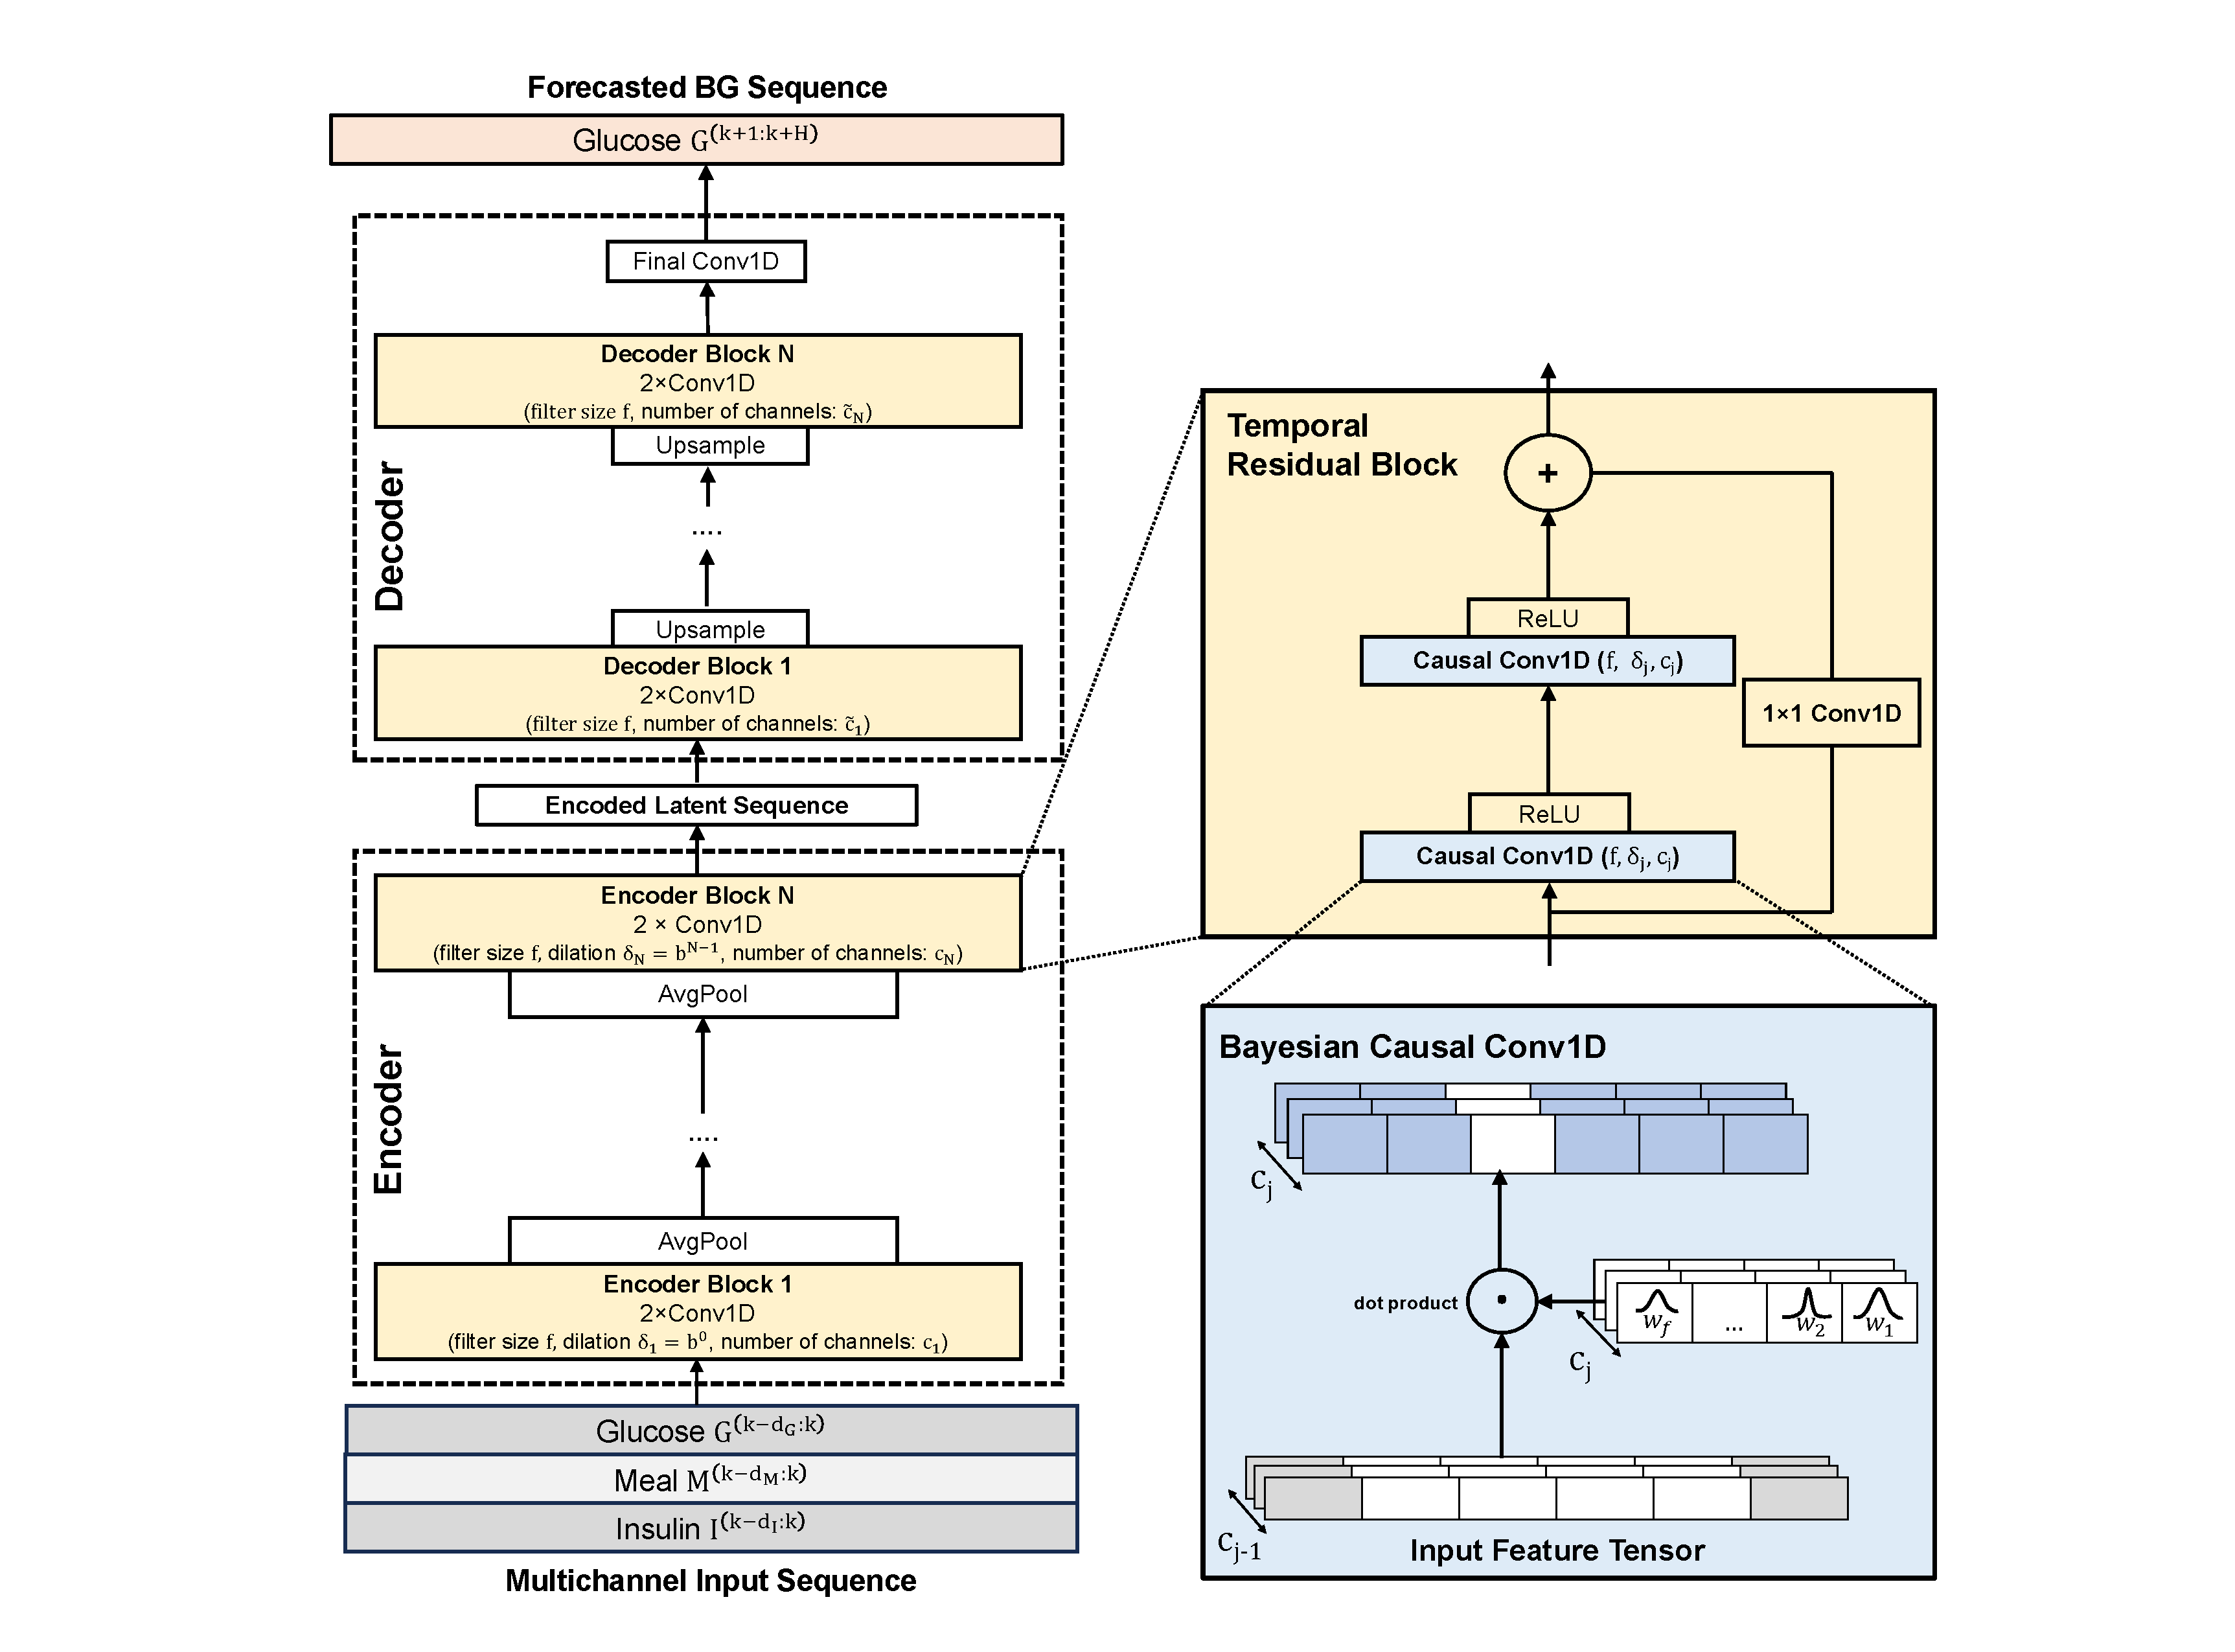
\includegraphics[width=1\linewidth]{Figures/results/full_archi.pdf}
    \caption{B-TCN architecture for blood glucose prediction}
    \label{fig:arch}
\end{figure}


Bayesian parameterization enters through the convolutional weights. In B-TCN, each scalar weight is treated as a random variable and is represented by a Gaussian variational posterior with two learned parameters: a mean and a standard deviation. Collecting all weights, the variational distribution is parameterized by $\eta=\{\mu_{\mathrm{post},i},\sigma_{\mathrm{post},i}\}_{i=1}^{p}$ for $p$ total weights. Training performs approximate Bayesian inference to fit these parameters so the resulting weight distribution both explains the data and remains close to the prior. At inference time, uncertainty is propagated by sampling weights from the learned variational distribution and running multiple stochastic forward passes; the predictive mean trajectory is obtained by averaging these passes, and predictive uncertainty is quantified from their variance. Batch normalization and dropout are not used in the B-TCN blocks as B-TCN already regularizes through the prior and learns calibrated epistemic uncertainty directly through the posterior over weights.


%++++++++++++++++++++++++++++++++++++++++++++++++++++++++++++++++++++++++
\subsection{Hierarchical Bayesian training}\label{sec:hierar_bayes}

Building upon MacKay’s evidence framework \cite{mackay1995probable}, as formalized in \cite{singh2024framework}, the parameters of the TCN models into three classes:\\
(i) Trainable weight parameters $w$,\\
(ii) Inference hyper-parameters $\sigma=[\sigma_{\mathrm{pr}}^{2},\,\sigma_{\mathrm{noise}}^{2}]$,\\
(iii) Architecture hyper-parameters $\xi$ (e.g., number of convolutional layers/blocks, dilation base, kernel size, and channel schedules).\\
Following hierarchical Bayesian inference, the evidence at each level acts as the likelihood for the next level:
\begin{align}
\text{Level 1:}\quad
\pi_{\mathrm{post}}(w\mid \mathcal{D},\sigma,\xi)
&=
\frac{\pi_{\mathrm{like}}(\mathcal{D}\mid w,\sigma,\xi)\,\pi_{\mathrm{pr}}(w\mid \sigma,\xi)}
{\pi_{\mathrm{evid}}(\mathcal{D}\mid \sigma,\xi)},
\label{eq:level1}
\\
\text{Level 2:}\quad
\pi_{\mathrm{post}}(\sigma\mid \mathcal{D},\xi)
&=
\frac{\pi_{\mathrm{evid}}(\mathcal{D}\mid \sigma,\xi)\,\pi_{\mathrm{pr}}(\sigma\mid \xi)}
{\pi_{\mathrm{evid}}(\mathcal{D}\mid \xi)},
\label{eq:level2}
\\
\text{Level 3:}\quad
\rho=\pi_{\mathrm{post}}(\xi\mid \mathcal{D})
&=
\frac{\pi_{\mathrm{evid}}(\mathcal{D}\mid \xi)\,\pi_{\mathrm{pr}}(\xi)}{\pi_{\mathrm{evid}}(\mathcal{D})}.
\label{eq:hirar}
\end{align}

Solution to each level of inference is given below:
\paragraph{Level 1 Weight parameters $\bs w$}
We approximate the intractable weight posterior with a mean-field Gaussian variational distribution
\begin{equation}
q_\eta(w)=\mathcal{N}\!\Big(\mu_{\mathrm{post}},\,\mathrm{diag}\big([\sigma_{\mathrm{post},i}^{2}]_{i=1}^{p}\big)\Big),
\qquad
\eta=\{\mu_{\mathrm{post},i},\sigma_{\mathrm{post},i}\}_{i=1}^{p},
\end{equation}
and compute $\eta_{\mathrm{opt}}$ by minimizing the negative ELBO (for fixed $\sigma$ and $\xi$):
\begin{equation}
\eta_{\mathrm{opt}}=\arg\min_{\eta}\,\mathcal{L}_{\mathrm{VI}}(\eta),
\end{equation}
with objective
\begin{equation}
\mathcal{L}_{\mathrm{VI}}(\eta)=
\mathrm{KL}\!\Big(q_\eta(w)\,\big\|\,\pi_{\mathrm{pr}}(w)\Big)
+\frac{N_f}{2}\log\!\big(2\pi\sigma_{\mathrm{noise}}^{2}\big)
+\frac{1}{M_{\mathrm{MC}}}\sum_{j=1}^{M_{\mathrm{MC}}}
\frac{1}{2\sigma_{\mathrm{noise}}^{2}}
\left\|G^{(k+1:k+K_f)}-G^{(k+1:k+K_f)}_{\mathrm{TCN}}(\hat w^{(j)})\right\|_2^{2},
\label{eq:lvi}
\end{equation}
where $\hat w^{(j)}\sim q_\eta(w)$ are Monte Carlo samples, $M_{\mathrm{MC}}$ is the number of samples, and $N_f$ denotes the total number of scalar forecast observations in $\mathcal{D}$.

\paragraph{Level 2 Inference hyper-parameters $\boldsymbol{\sigma}} Given the variational posterior from Level 1, we compute the MAP hyper-parameters by maximizing the log-evidence
\begin{equation}
\sigma_{\mathrm{opt}}=\arg\max_{\sigma}\,\mathcal{L}_{\mathrm{Evid2}}(\sigma),
\end{equation}
where the log-evidence for fixed architecture $\xi$ is
\begin{align}
\mathcal{L}_{\mathrm{Evid2}}(\sigma)
=\log \pi_{\mathrm{evid}}(\mathcal{D}\mid \sigma,\xi)
\approx\;&
-\frac{1}{2\sigma_{\mathrm{noise}}^{2}}
\sum_{k=1}^{N}
\left\|G^{(k+1:k+K_f)}-G^{(k+1:k+K_f)}_{\mathrm{TCN}}(\mu_{\mathrm{post}})\right\|_2^{2}
-\frac{N_f}{2}\log\!\big(2\pi\sigma_{\mathrm{noise}}^{2}\big)
\nonumber\\
&-\frac{1}{2\sigma_{\mathrm{pr}}^{2}}\|\mu_{\mathrm{post}}\|_2^{2}
-\frac{p}{2}\log\!\big(2\pi\sigma_{\mathrm{pr}}^{2}\big)
-\frac{1}{2}\log\det(H),
\label{eq:levid2}
\end{align}
with $p$ the number of weights and $H$ the Hessian of the negative log-posterior in $w$ evaluated at $w=\mu_{\mathrm{post}}$.
Under the mean-field VI approximation, we use the diagonal covariance returned by VI to approximate
\begin{equation}
H^{-1}\approx \mathrm{diag}([\sigma_{\mathrm{post},i}^{2}]_{i=1}^{p}),
\qquad
\log\det(H)\approx \sum_{i=1}^{p}\log(\sigma_{\mathrm{post},i}^{2}).
\end{equation}
In practice, Levels 1--2 are implemented by alternating updates: (i) fix $\sigma$ and solve \eqref{eq:lvi} for $\eta$, then (ii) fix $(\mu_{\mathrm{post}},\sigma_{\mathrm{post}})$ and update $\sigma$ by maximizing \eqref{eq:levid2}, repeated until convergence.

\paragraph{Level 3 Infer the architecture hyper-parameters $\bs \xi$}
To compare candidate architectures, we form the marginal evidence by integrating out $\sigma$ around $\sigma_{\mathrm{opt}}$:
\begin{equation}
\mathrm{Evid3}
=
\pi_{\mathrm{evid}}(\mathcal{D}\mid \xi)
=
\pi_{\mathrm{evid}}(\mathcal{D}\mid \sigma_{\mathrm{opt}},\xi)\,
\pi_{\mathrm{pr}}(\sigma_{\mathrm{opt}}\mid \xi)\,
\Big[2\pi\sqrt{\mathrm{Var}(\sigma_{\mathrm{pr}}^{2})\,\mathrm{Var}(\sigma_{\mathrm{noise}}^{2})}\Big].
\label{eq:evid3}
\end{equation}
Assuming a uniform prior over architectures, the posterior plausibility reduces to normalized evidence over a finite candidate set
$\mathcal{M}_{\mathrm{predict}}=\{\xi_m\}_{m=1}^{M}$:
\begin{equation}
\rho_m
=
\frac{\pi_{\mathrm{evid}}(\mathcal{D}\mid \xi_m)}
{\sum_{j=1}^{M}\pi_{\mathrm{evid}}(\mathcal{D}\mid \xi_j)},
\qquad
m=1,\ldots,M,
\label{eq:rho}
\end{equation}
and the selected architecture is $\xi_{\mathrm{opt}}=\arg\max \rho_m$.




%++++++++++++++++++++++++++++++++++++++++++++++++++++++++++++++++++++++++
\subsection{Model discovery framework XXXX}\label{sec:opal}

\begin{figure} [H]
    \centering
    \includegraphics[width=0.75\linewidth]{Figures/results/OPAL_tcn.png}
    \caption{Model discovery framework}
    \label{fig:opal}
\end{figure}

\autoref{fig:opal} summarizes the evidence-driven workflow used to systematically discover digital-twin (DT)-ready B-TCN architectures from a large design space. The goal is to identify predictive models that (i) map recent multi-channel histories of glucose, meals, and insulin to a future glucose trajectory, and (ii) remain credible under uncertainty when evaluated on validation patients. We begin by constructing an initial feasible set of candidate architectures using biological constraints. To explicitly control the complexity search, candidates are grouped into categories (bins) by their number of parameters. 
For a fixed Occam category $l$, we train each architecture $\xi_m$ using the hierarchical Bayesian procedure in \autoref{sec:hierar_bayes}. We perform variational inference to obtain a mean-field posterior over weights, then estimate inference hyperparameters (e.g., $\sigma_{\text{noise}}$ and $\sigma_{\text{pr}}$) and finally compute their model plausibility. This training-and-ranking step is repeated across all cross-validation folds. The most plausible models from each fold are subject to validation under uncertainty with specific tolearnce.  
If no model in category $l$ passes validation, the framework advances to the next Occam category ($l \leftarrow l+1$) and repeats training, plausibility ranking, and validation. If the final category is reached without success, the workflow returns to expand the candidate model set with new set of candidate models. 







%========================================================
% Results
%========================================================
\section{Results}\label{sec:results}
In this section, we present results from XXXXXXX

%++++++++++++++++++++++++++++++++++++++++++++++++++++++++++++++++++++++++
\subsection{Bayesian TCN and plausibility results}
\begin{itemize}
    \item Training data and how generated with minimal Bergman’s model description => mimicking CGM data

The glucose--insulin dynamics in the first set of data shown in \autoref{fig:bergman} are represented by the Bergman minimal model \cite{bergman1981physiologic}, with meal disturbances introduced via the Dalla Man gut absorption model \cite{dalla2006system}. The Bergman states are plasma glucose $G(t)$ [mg/dL], remote insulin action $X(t)$ [min$^{-1}$], and plasma insulin $I(t)$ [mU/L], with basal values $G_b$ and $I_b$. For a Type-1 diabetic (T1D) subject, endogenous pancreatic secretion is removed and insulin is administered externally. The stabilized T1D model is
\begin{align}
\dot G(t) &= -\big(X(t)+p_1\big)\,G(t) + p_1 G_b + \frac{R_{ag}(t)}{V_g}, \label{eq:t1d_bergman_G}\\
\dot X(t) &= -p_2 X(t) + p_3\big(I(t)-I_b\big), \label{eq:t1d_bergman_X}\\
\dot I(t) &= -p_4\big(I(t)-I_b\big) + U(t), \label{eq:t1d_bergman_I}
\end{align}
where $V_g$ [dL] is the glucose distribution volume and $U(t)$ is the insulin control input around basal. This form is obtained by writing the physical infusion as
\begin{equation}
U_0(t) = U(t) + p_4 I_b,
\end{equation}
so that $p_4 I_b$ mimics the basal insulin dose required to prevent the open-loop glucose drift in T1D.

Meal absorption is modeled with stomach--gut compartments whose output is $R_{ag}(t)$. Let $q_{\mathrm{sto}1}(t)$ and $q_{\mathrm{sto}2}(t)$ [mg] denote stomach glucose in solid and liquid phases, and $q_{\mathrm{gut}}(t)$ [mg] denote intestinal glucose. A meal of size $D$ [mg] consumed at time $t_m$ is injected using a Dirac impulse:
\begin{align}
\dot q_{\mathrm{sto}1}(t) &= -k_{21}\,q_{\mathrm{sto}1}(t) + D\,\delta(t-t_m), \label{eq:gut1}\\
\dot q_{\mathrm{sto}2}(t) &= -k_{\mathrm{empt}}\!\big(q_{\mathrm{sto}}(t)\big)\,q_{\mathrm{sto}2}(t) + k_{21}\,q_{\mathrm{sto}1}(t), \label{eq:gut2}\\
\dot q_{\mathrm{gut}}(t) &= -k_{\mathrm{abs}}\,q_{\mathrm{gut}}(t) + k_{\mathrm{empt}}\!\big(q_{\mathrm{sto}}(t)\big)\,q_{\mathrm{sto}2}(t), \label{eq:gut3}\\
R_{ag}(t) &= f\,k_{\mathrm{abs}}\,q_{\mathrm{gut}}(t), \qquad q_{\mathrm{sto}}(t)=q_{\mathrm{sto}1}(t)+q_{\mathrm{sto}2}(t), \label{eq:Ra}
\end{align}
where $k_{21}$ [min$^{-1}$] governs transfer from solid to liquid stomach phase, $k_{\mathrm{abs}}$ [min$^{-1}$] governs intestinal absorption, and $f$ is a dimensionless bioavailability factor. Gastric emptying is modeled as a smooth nonlinearity between $k_{\min}$ and $k_{\max}$:
\begin{align}
k_{\mathrm{empt}}(q_{\mathrm{sto}}) &=
k_{\min} + \tfrac12\big(k_{\max}-k_{\min}\big)\Big(
\tanh\!\big[\alpha(q_{\mathrm{sto}}-bD)\big]
-\tanh\!\big[\beta(q_{\mathrm{sto}}-cD)\big] + 2\Big), \label{eq:kempt}\\
\alpha &= \frac{5}{2D(1-b)}, \qquad
\beta  = \frac{5}{2Dc}, \label{eq:alpha_beta}
\end{align}
with $b,c\in(0,1)$ dimensionless shape parameters. 

\begin{table}[t]
\centering
\caption{Parameter values for the Type-1 diabetic patinet used in simulation.}
\label{tab:t1d_params}
\begin{tabular}{lll}
\hline
Parameter & Value & Units \\
\hline
$p_1$ & $0.028735$ & min$^{-1}$ \\
$p_2$ & $0.028344$ & min$^{-1}$ \\
$p_3$ & $5.035\times 10^{-5}$ & min$^{-2}\cdot$L/mU \\
$p_4$ & $5/54$ & min$^{-1}$ \\
$G_b$ & $119.1858$ & mg/dL \\
$I_b$ & $15.3872$ & mU/L \\
$V_g$ & $128.8237$ & dL \\
$k_{\max}$ & $0.0429$ & min$^{-1}$ \\
$k_{\min}$ & $0.0141$ & min$^{-1}$ \\
$k_{\mathrm{abs}}$ & $0.2062$ & min$^{-1}$ \\
$k_{21}$ & $0.0558$ & min$^{-1}$ \\
$b$ & $0.7612$ & -- \\
$c$ & $0.1372$ & -- \\
$f$ & $0.9$ & -- \\
$\gamma$ & N/A (T1D) & -- \\
$h$ & N/A (T1D) & mg/dL \\
\hline
\end{tabular}
\end{table}




\begin{figure}[H]
\centering
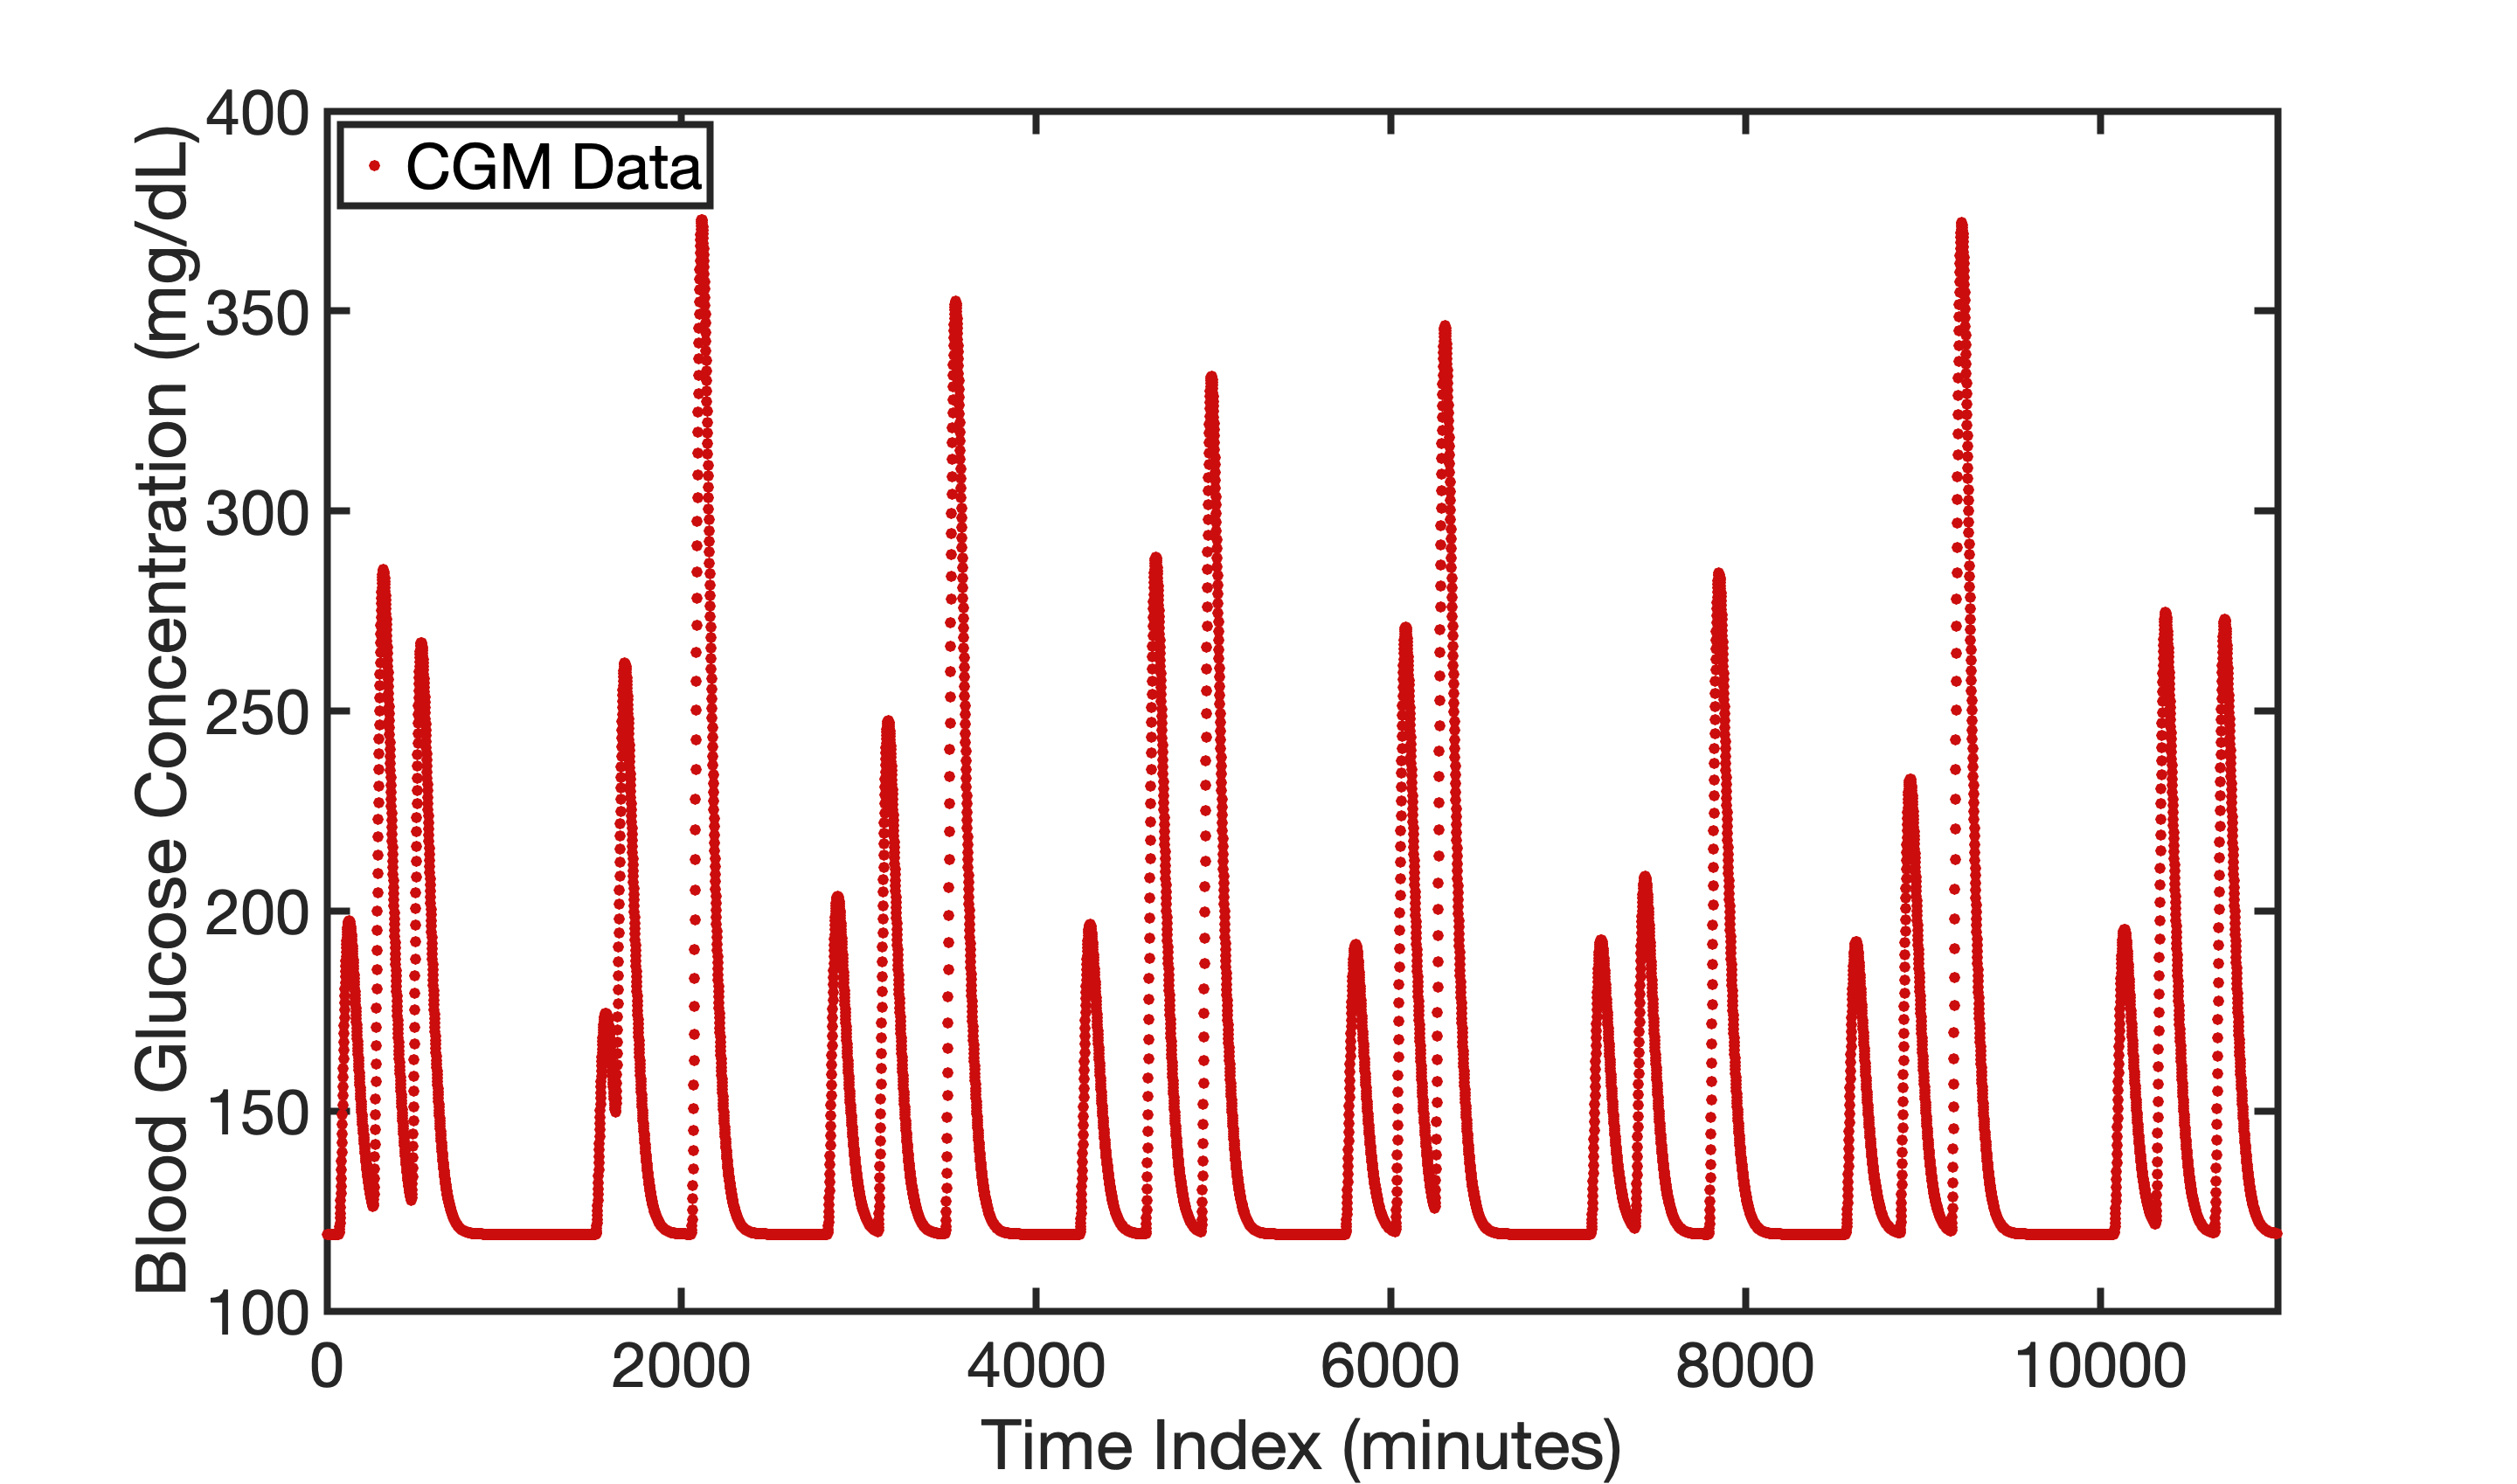
\includegraphics[width=\linewidth]{Figures/results/bergman_data.png}
\caption{Blood glucose data generated from Bergman minimal model}
\label{fig:bergman}
\end{figure}





   \item 2D plausibility and RF plots 

\autoref{fig:dil_evid}(a) reports the corresponding receptive field over the architecture parameters (number of temporal blocks an dilation base). Receptive field grows rapidly with both the number of blocks and dilation base. Similarly, \autoref{fig:dil_evid}(b) reports the number of trainable parameters over the architectural grid. Parameter count increases sharply with the number of temporal blocks (depth) and less dramatically with dilation base.

The evidence peak occurs in an intermediate receptive-field region, suggesting a practical operating point: the model must access sufficient temporal context to capture delayed meal and insulin effects, but excessively large receptive fields (driven by aggressive dilation and/or depth) do not provide consistent gains and can reduce effective utilization of informative local dynamics.

Figure~\autoref{fig:dil_evid}(c) summarizes the Bayesian log-evidence obtained from a grid search over Temporal Convolutional Network (TCN) architectures parameterized by dilation base and number of temporal blocks. The evidence surface is highly non-uniform: a small subset of architectures achieves substantially higher evidence (warmer colors), while many alternatives are strongly penalized (cooler colors). This pattern indicates that only a narrow design region provides a favorable balance between data-fit and model complexity for glucose forecasting.




   
\begin{figure}[H]
\centering

\begin{minipage}[t]{0.45\textwidth}
  \centering
  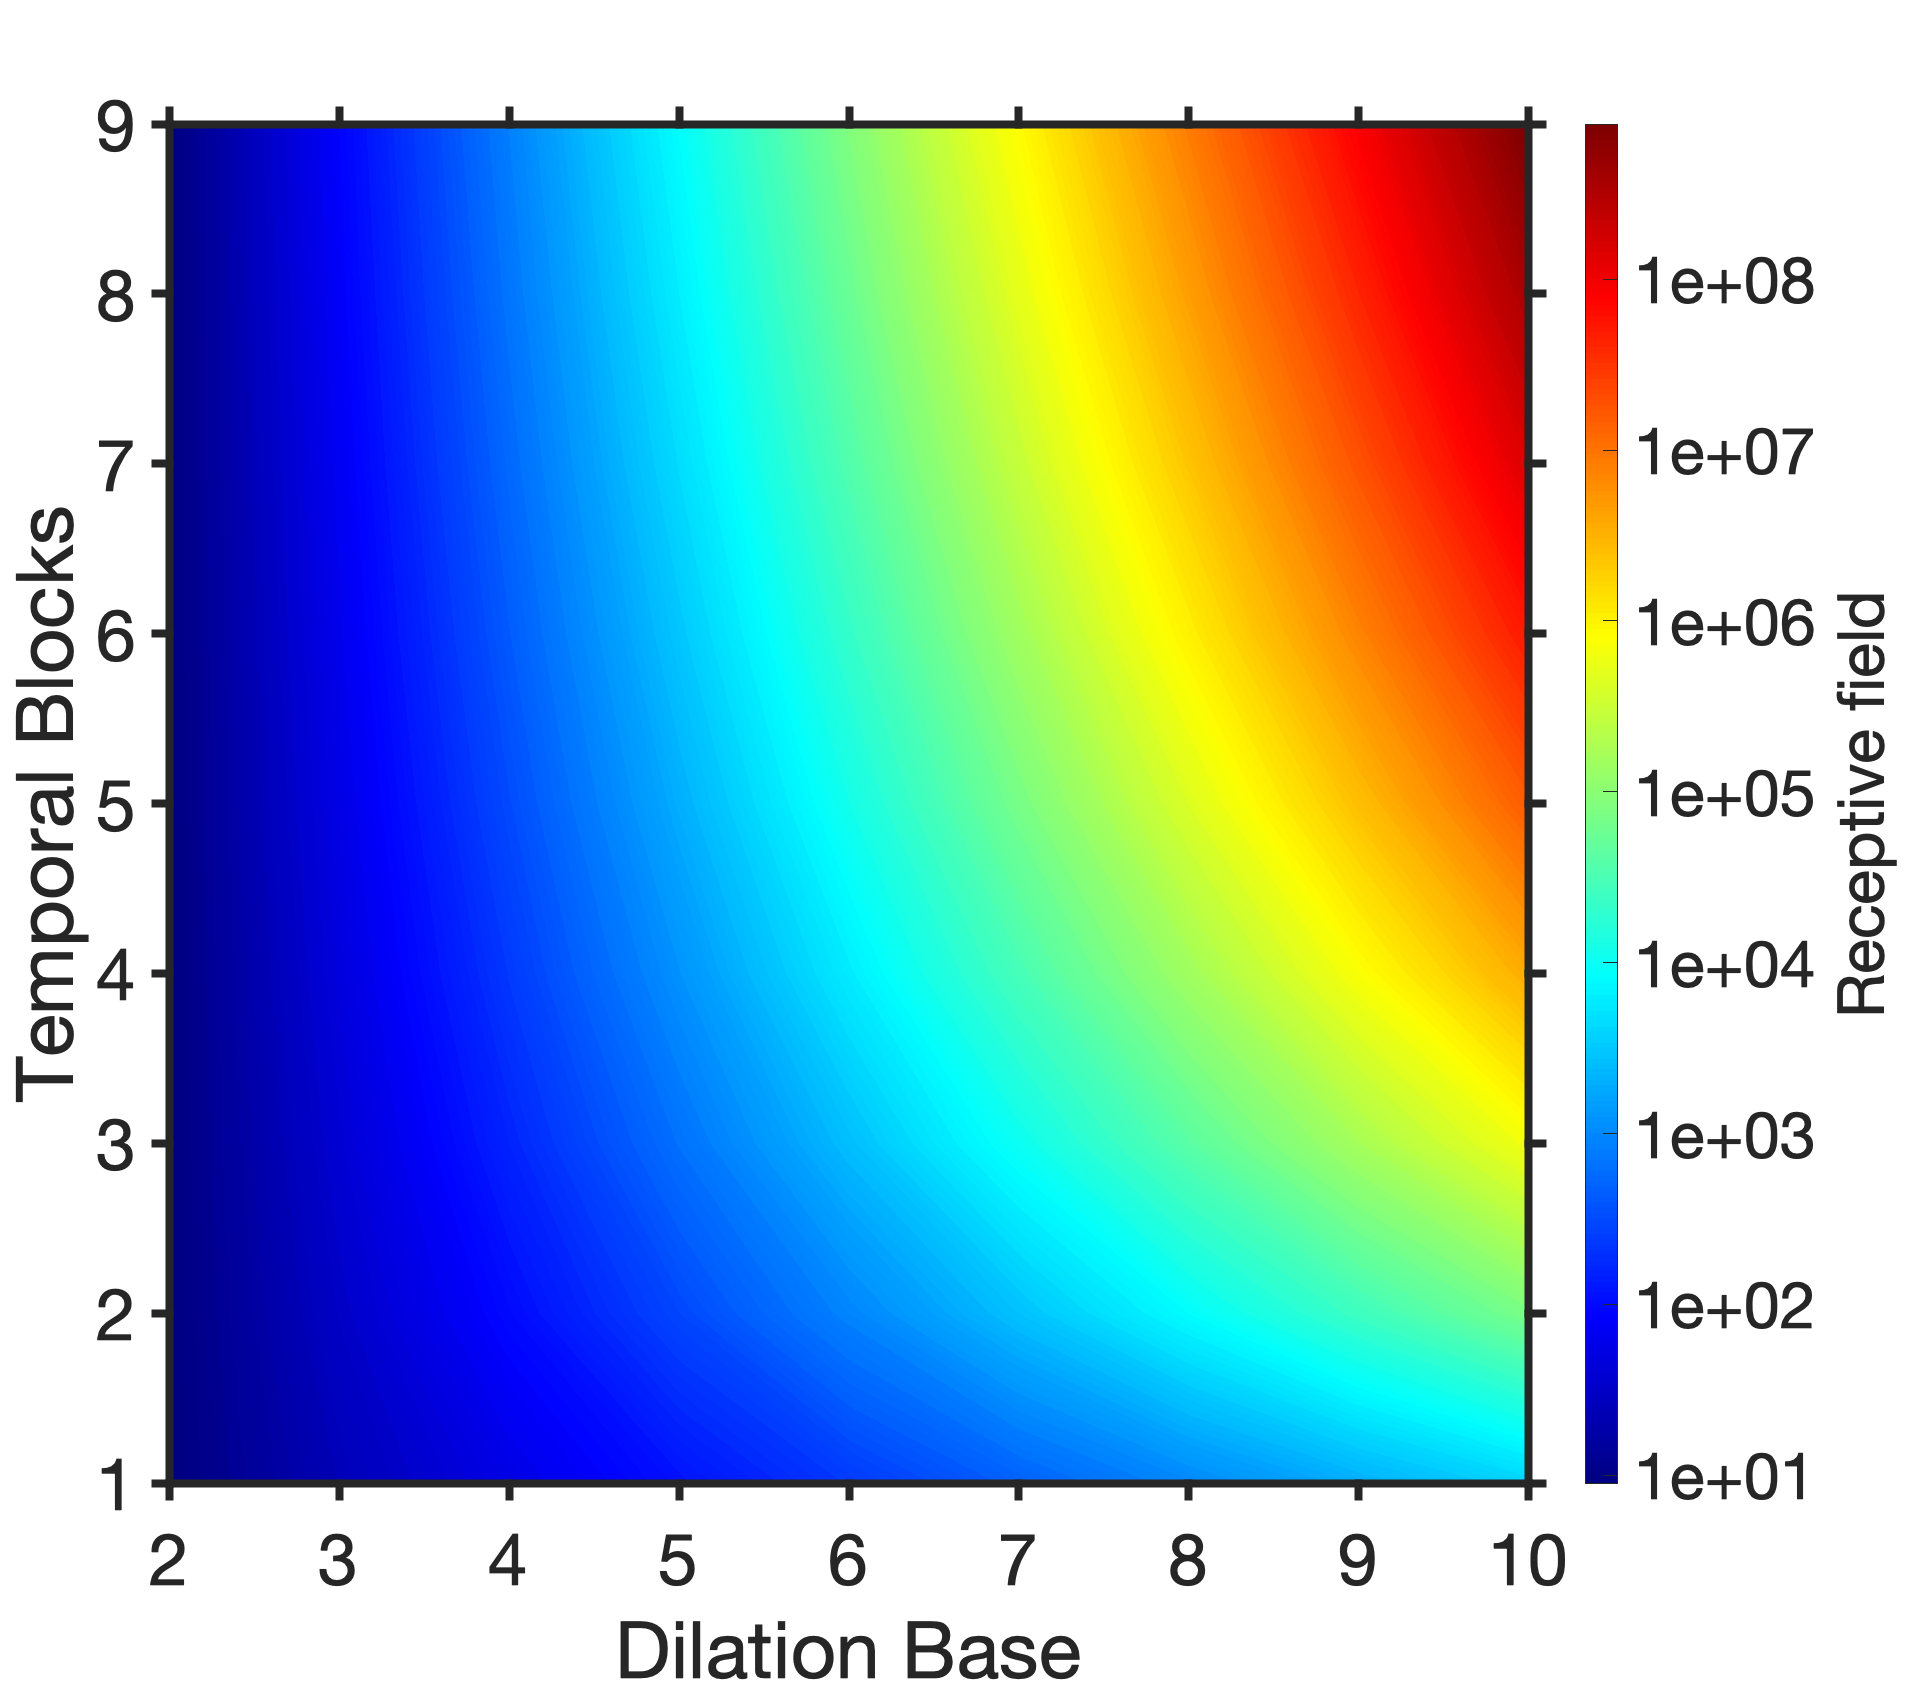
\includegraphics[width=\linewidth]{Figures/results/temp_dil_rf.png}
  \caption*{(a)}
\end{minipage}
\begin{minipage}[t]{0.43\textwidth}
  \centering
  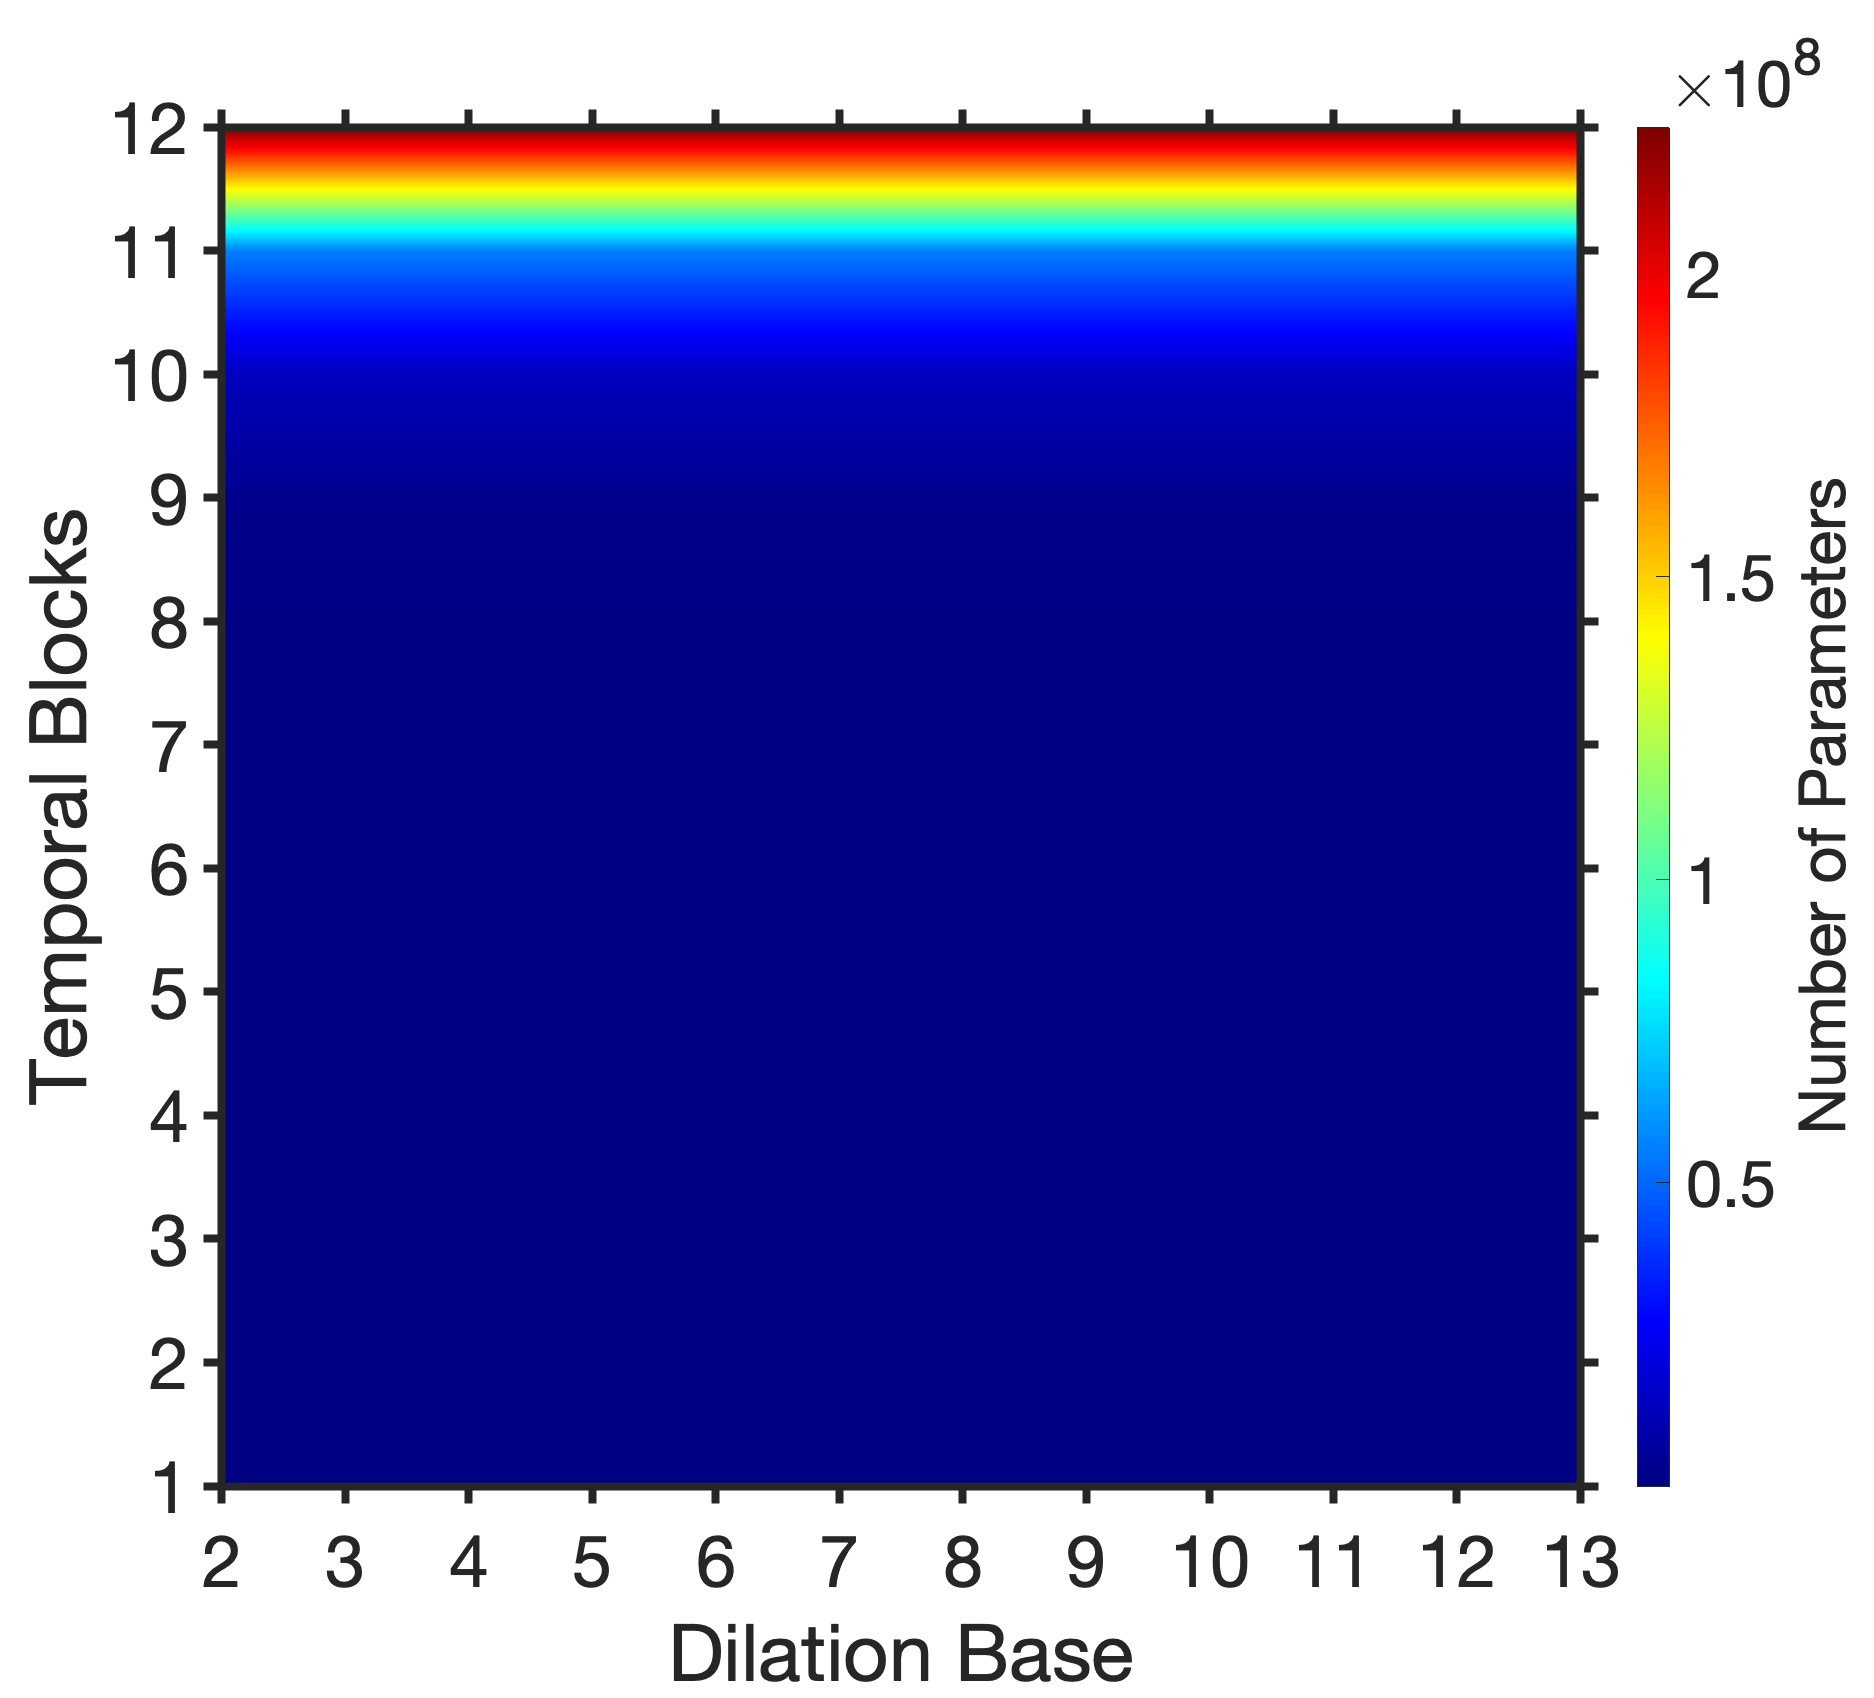
\includegraphics[width=\linewidth]{Figures/results/temp_dil_param.png}
  \caption*{(b)}
\end{minipage}

\begin{minipage}[t]{\textwidth}
  \centering
  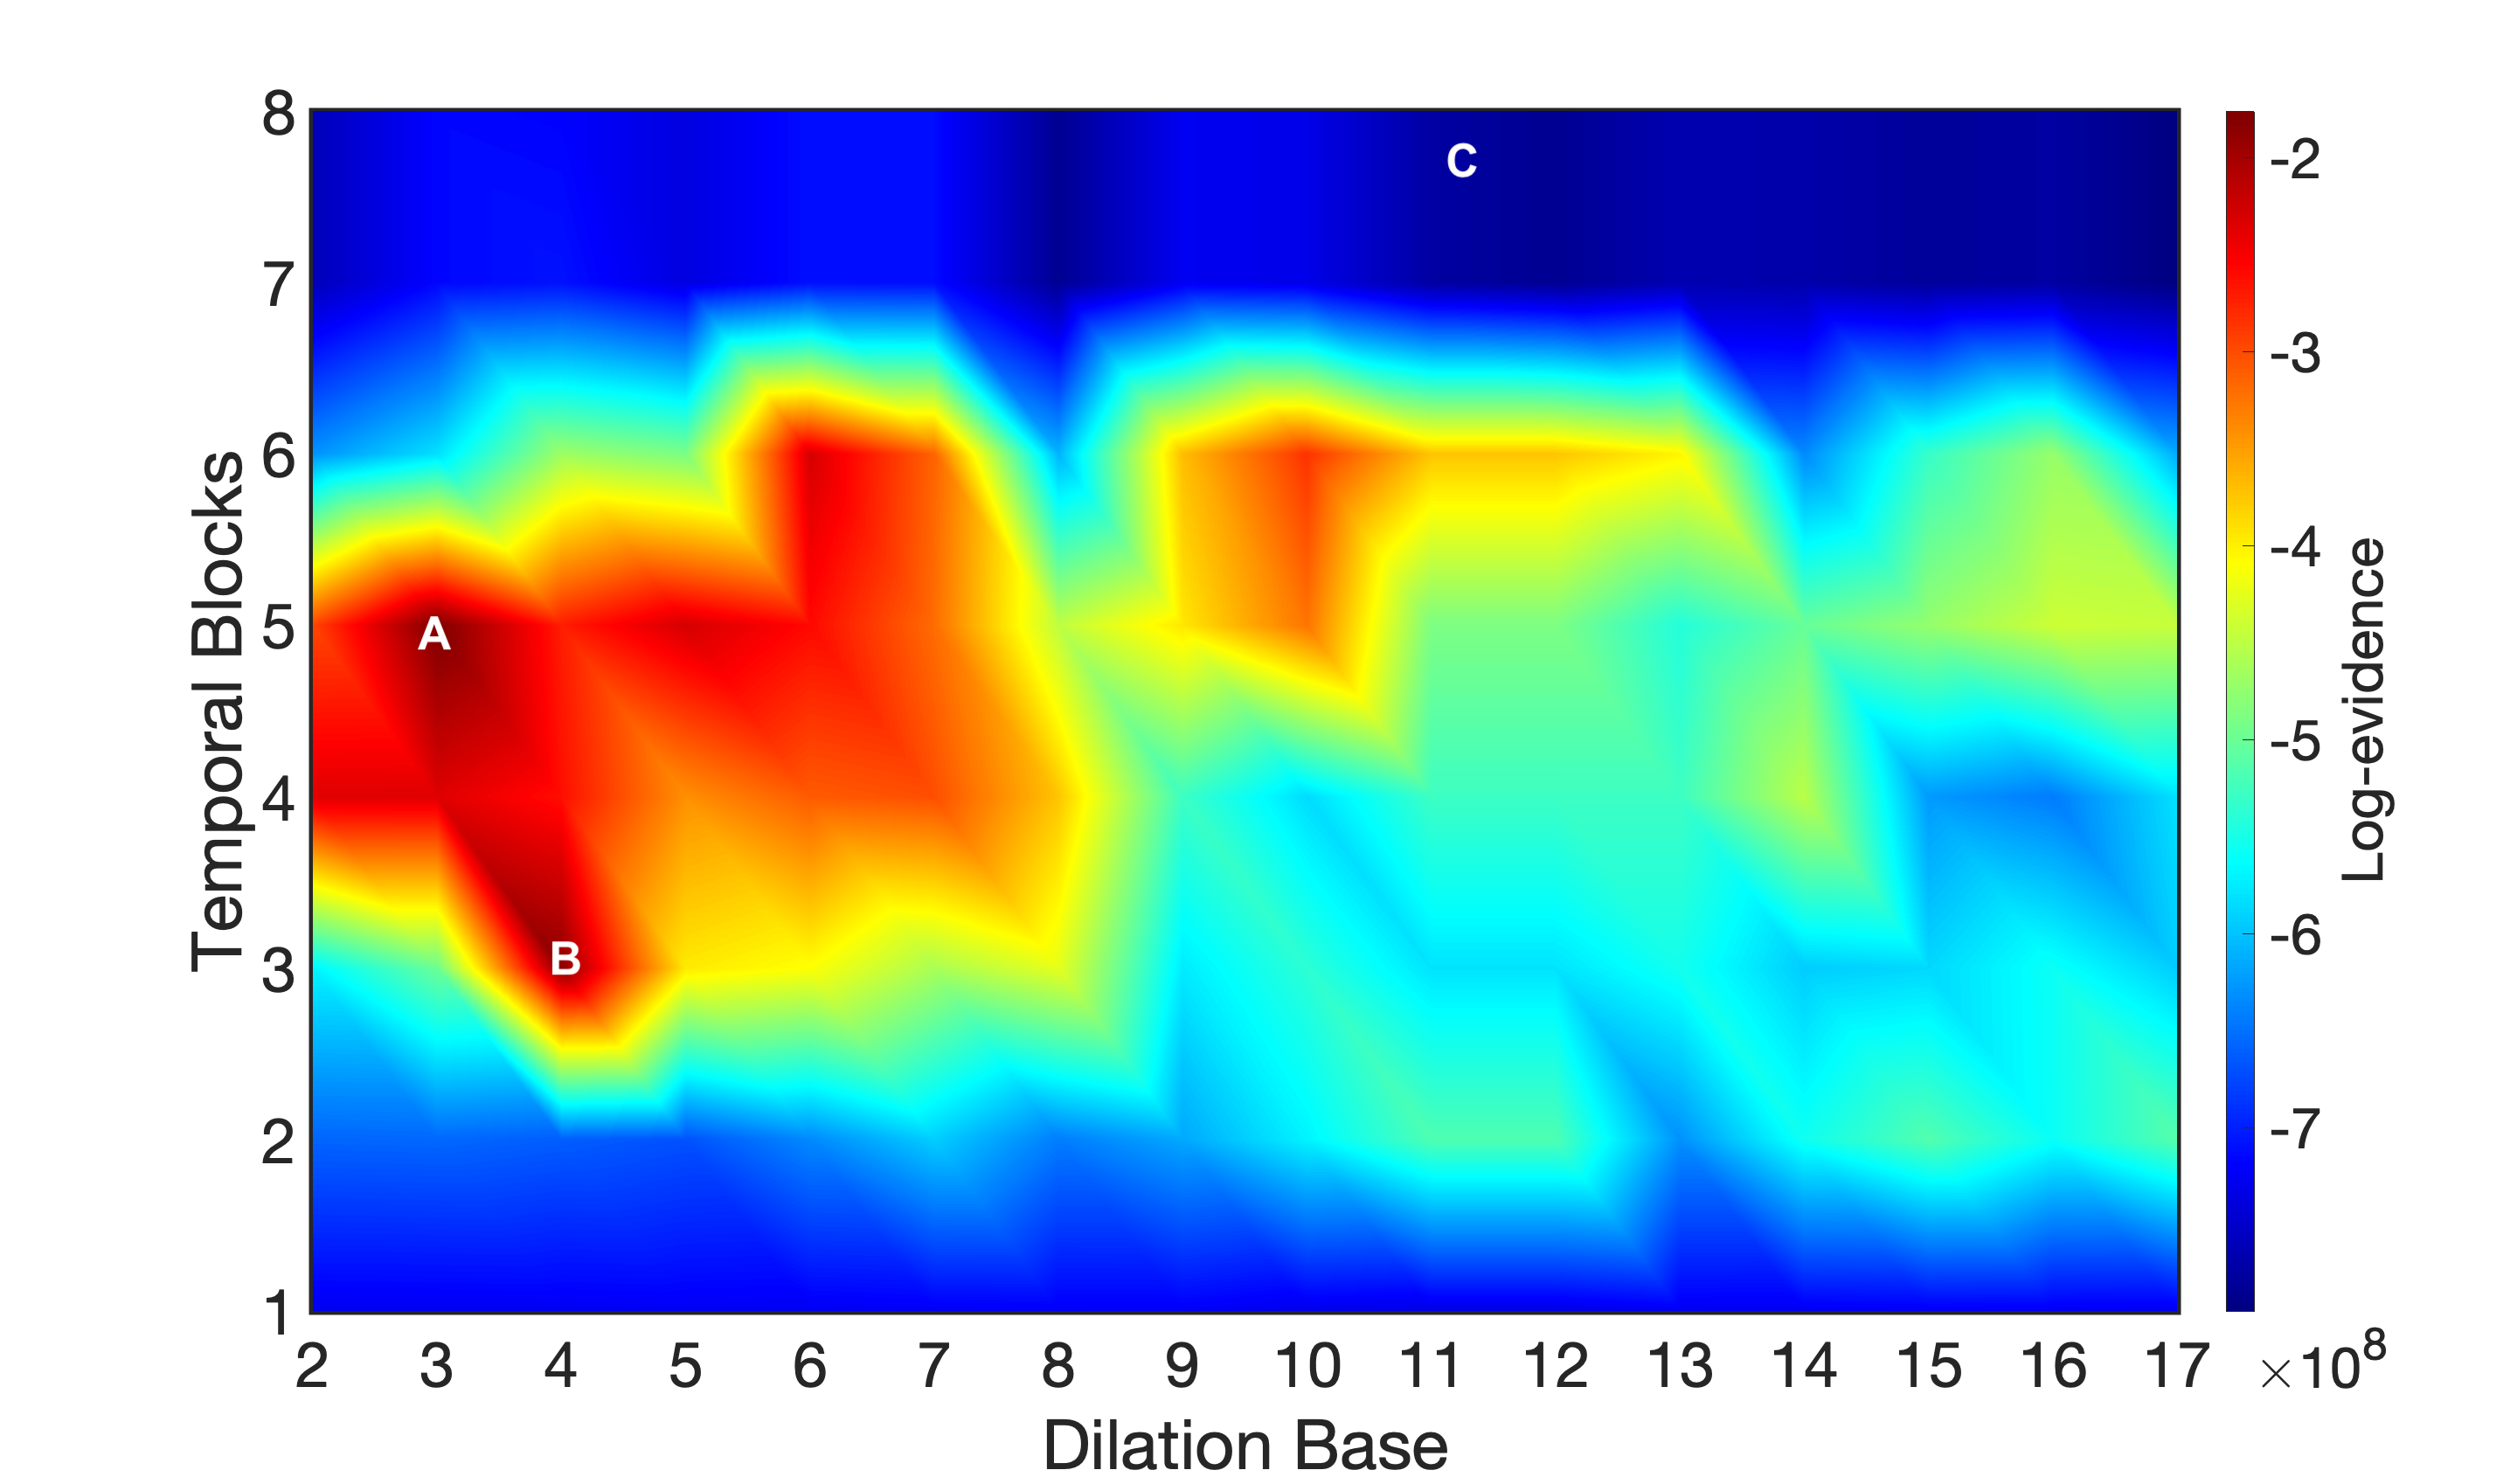
\includegraphics[width=\linewidth]{Figures/results/temp_dil_evid.png}
  \caption*{(c)}
\end{minipage}

\caption{Relationship between different architecture hyper-parameters and their $2^{nd}$ log-evidence value.  (a) Contour plot of temporal blocks, dilation base and receptive field, (b) Contour plot of temporal blocks, dilation base and number of parameters, and (c) Contour plot of Temporal blocks, dilation base and evidence.}
\label{fig:dil_evid}
\end{figure}

   \item Training/prediction results including NLPD equation and values (whole data and prediction) => conclusion: higher plausibility results in better prediction

\autoref{fig:trains} connects the evidence ranking to qualitative predictive performance using three representative architectures (A, B, and C) selected from distinct regions of the evidence plot. Architectures A and B (high-evidence) exhibit strong agreement with CGM data during training and maintain accurate short-horizon forecasts with uncertainty bands that remain concentrated around the predicted trajectory. In contrast, architecture C (low-evidence) shows visibly weaker peak tracking and degraded forecast behavior. These examples support the interpretation that higher evidence corresponds to models that generalize better in prediction, not merely models that fit training trajectories. 


\begin{figure}[H]
\centering

\begin{minipage}[t]{0.33\textwidth}
  \centering
  \includegraphics[width=\linewidth]{Figures/results/train_pointA.png}
  \caption*{(a)}
\end{minipage}%
\hfill
\begin{minipage}[t]{0.33\textwidth}
  \centering
  \includegraphics[width=\linewidth]{Figures/results/train_pointB.png}
  \caption*{(b)}
\end{minipage}%
\hfill
\begin{minipage}[t]{0.33\textwidth}
  \centering
  \includegraphics[width=\linewidth]{Figures/results/train_pointC.png}
  \caption*{(c)}
\end{minipage}

\begin{minipage}[t]{0.33\textwidth}
  \centering
  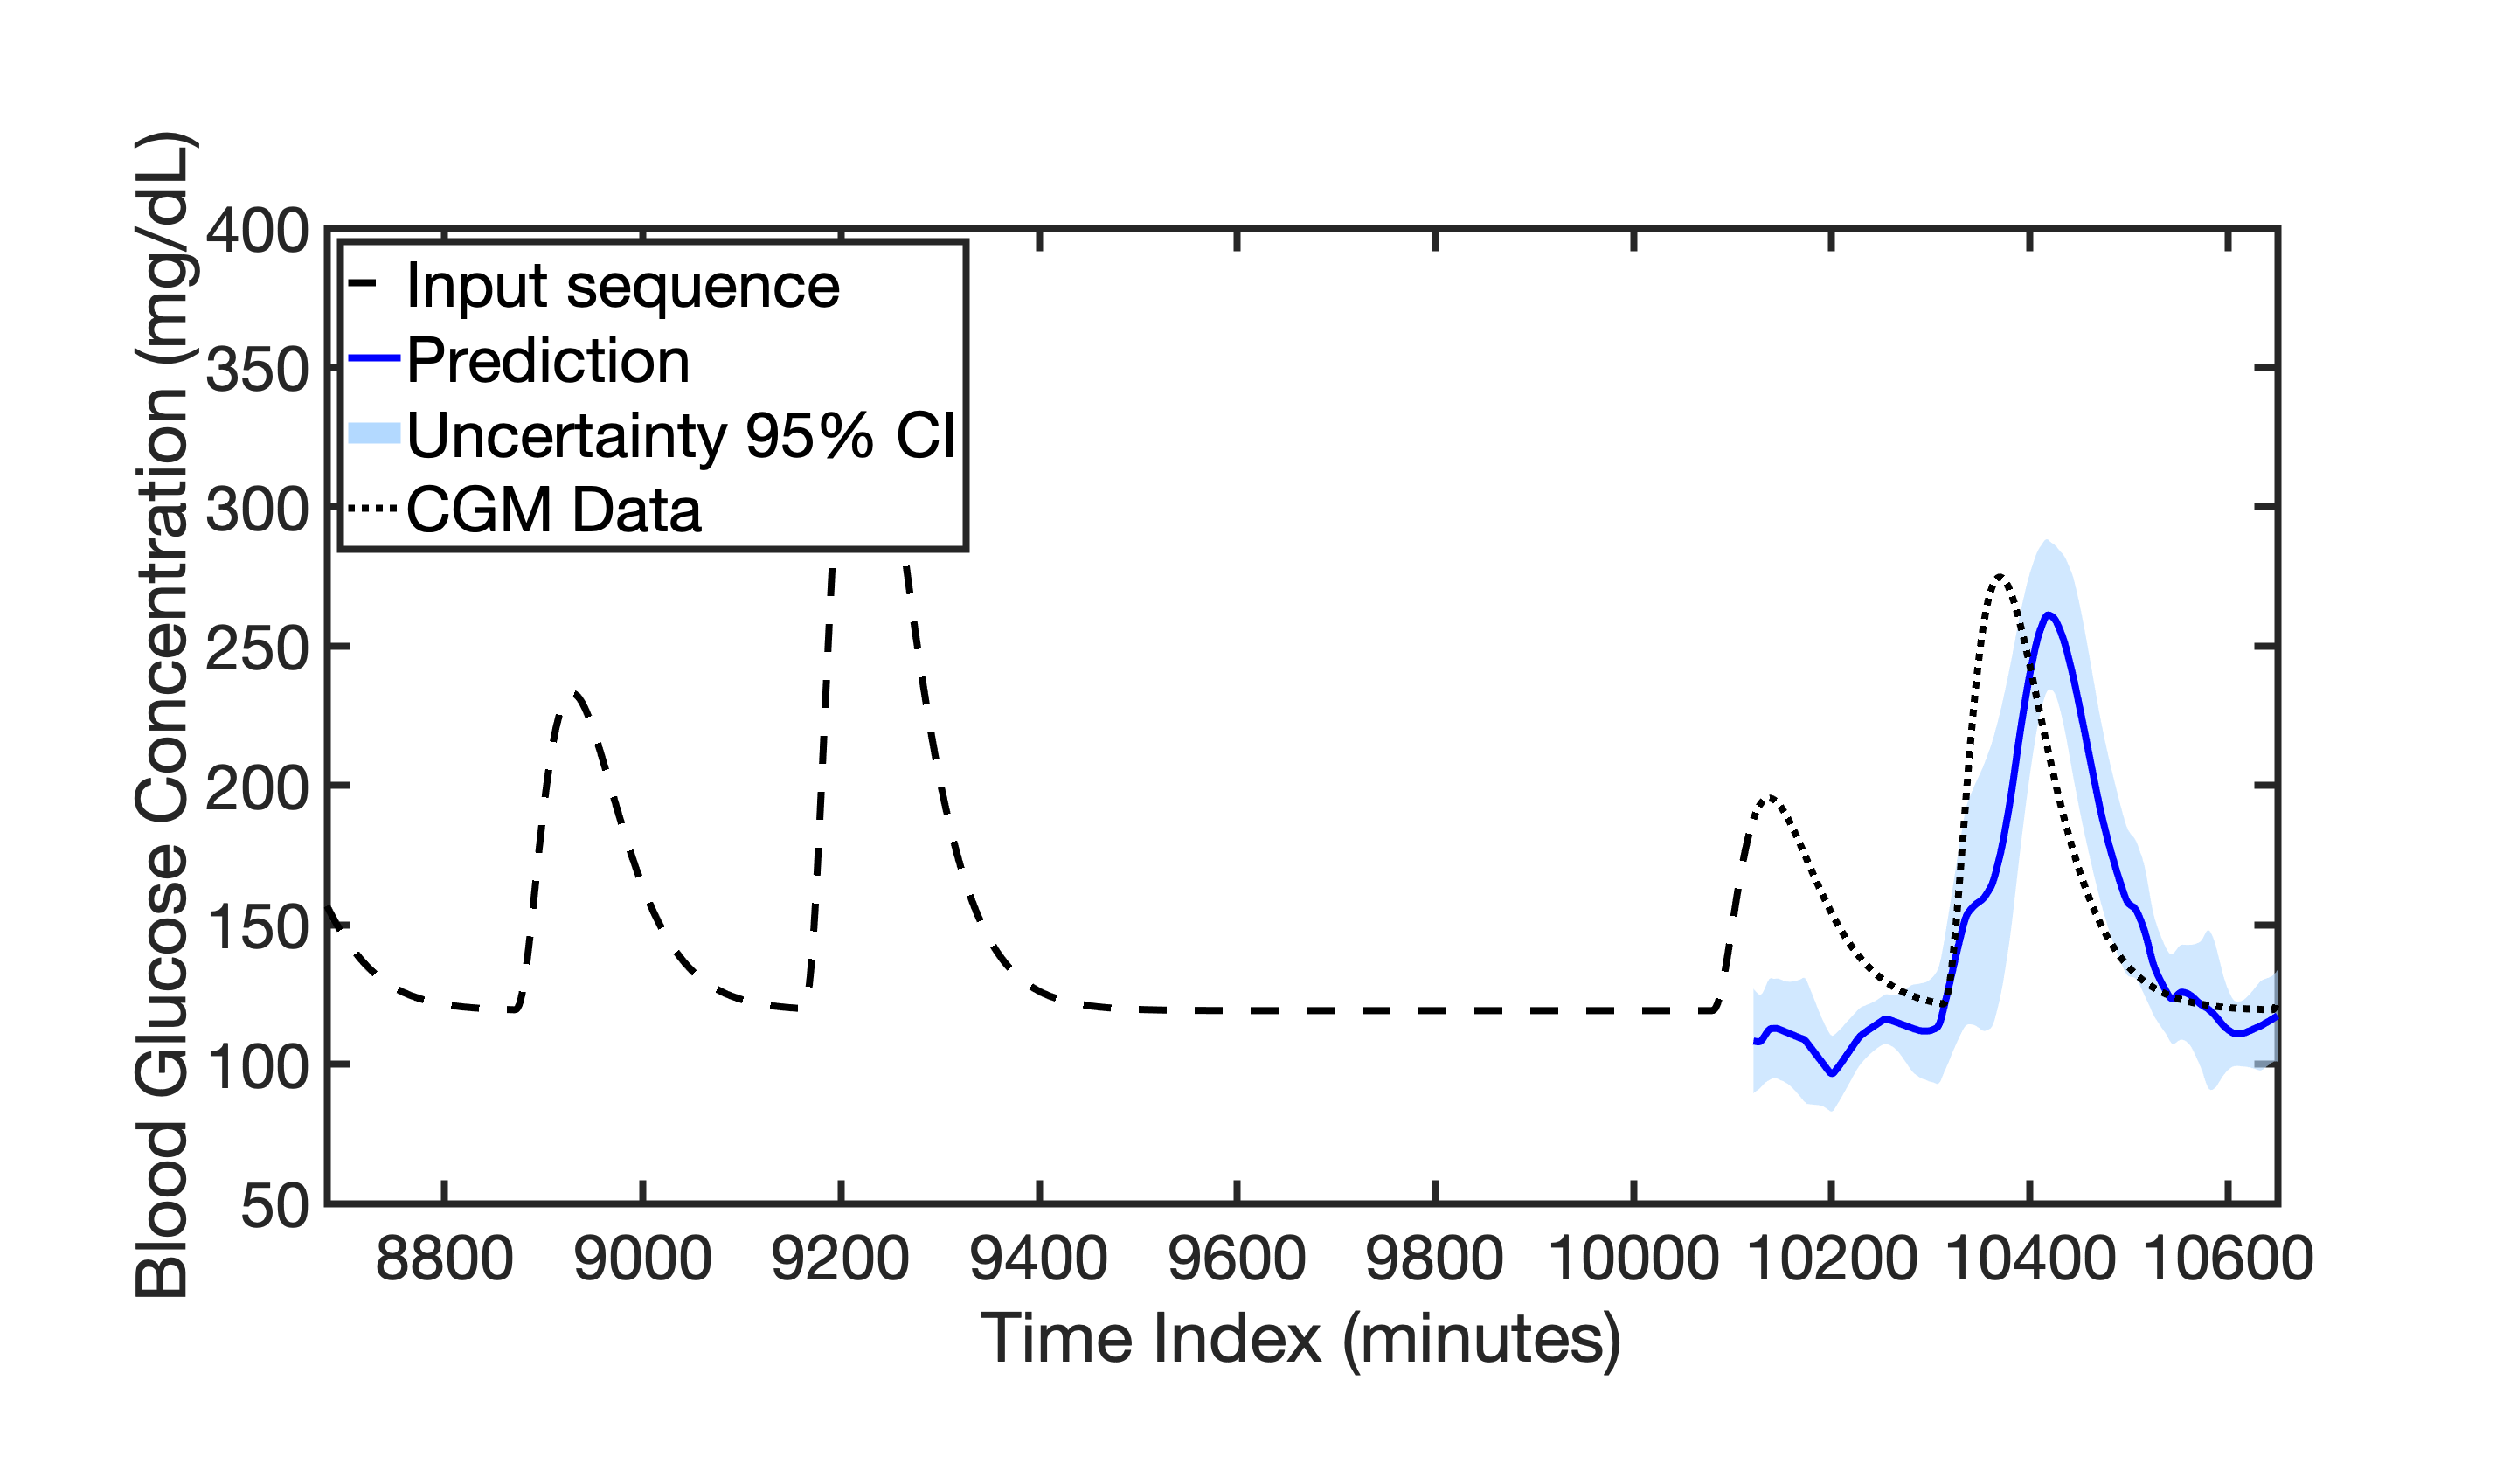
\includegraphics[width=\linewidth]{Figures/results/pred_pointA.png} % pred_good.png ?
  \caption*{(d)}
\end{minipage}%
\hfill
\begin{minipage}[t]{0.33\textwidth}
  \centering
  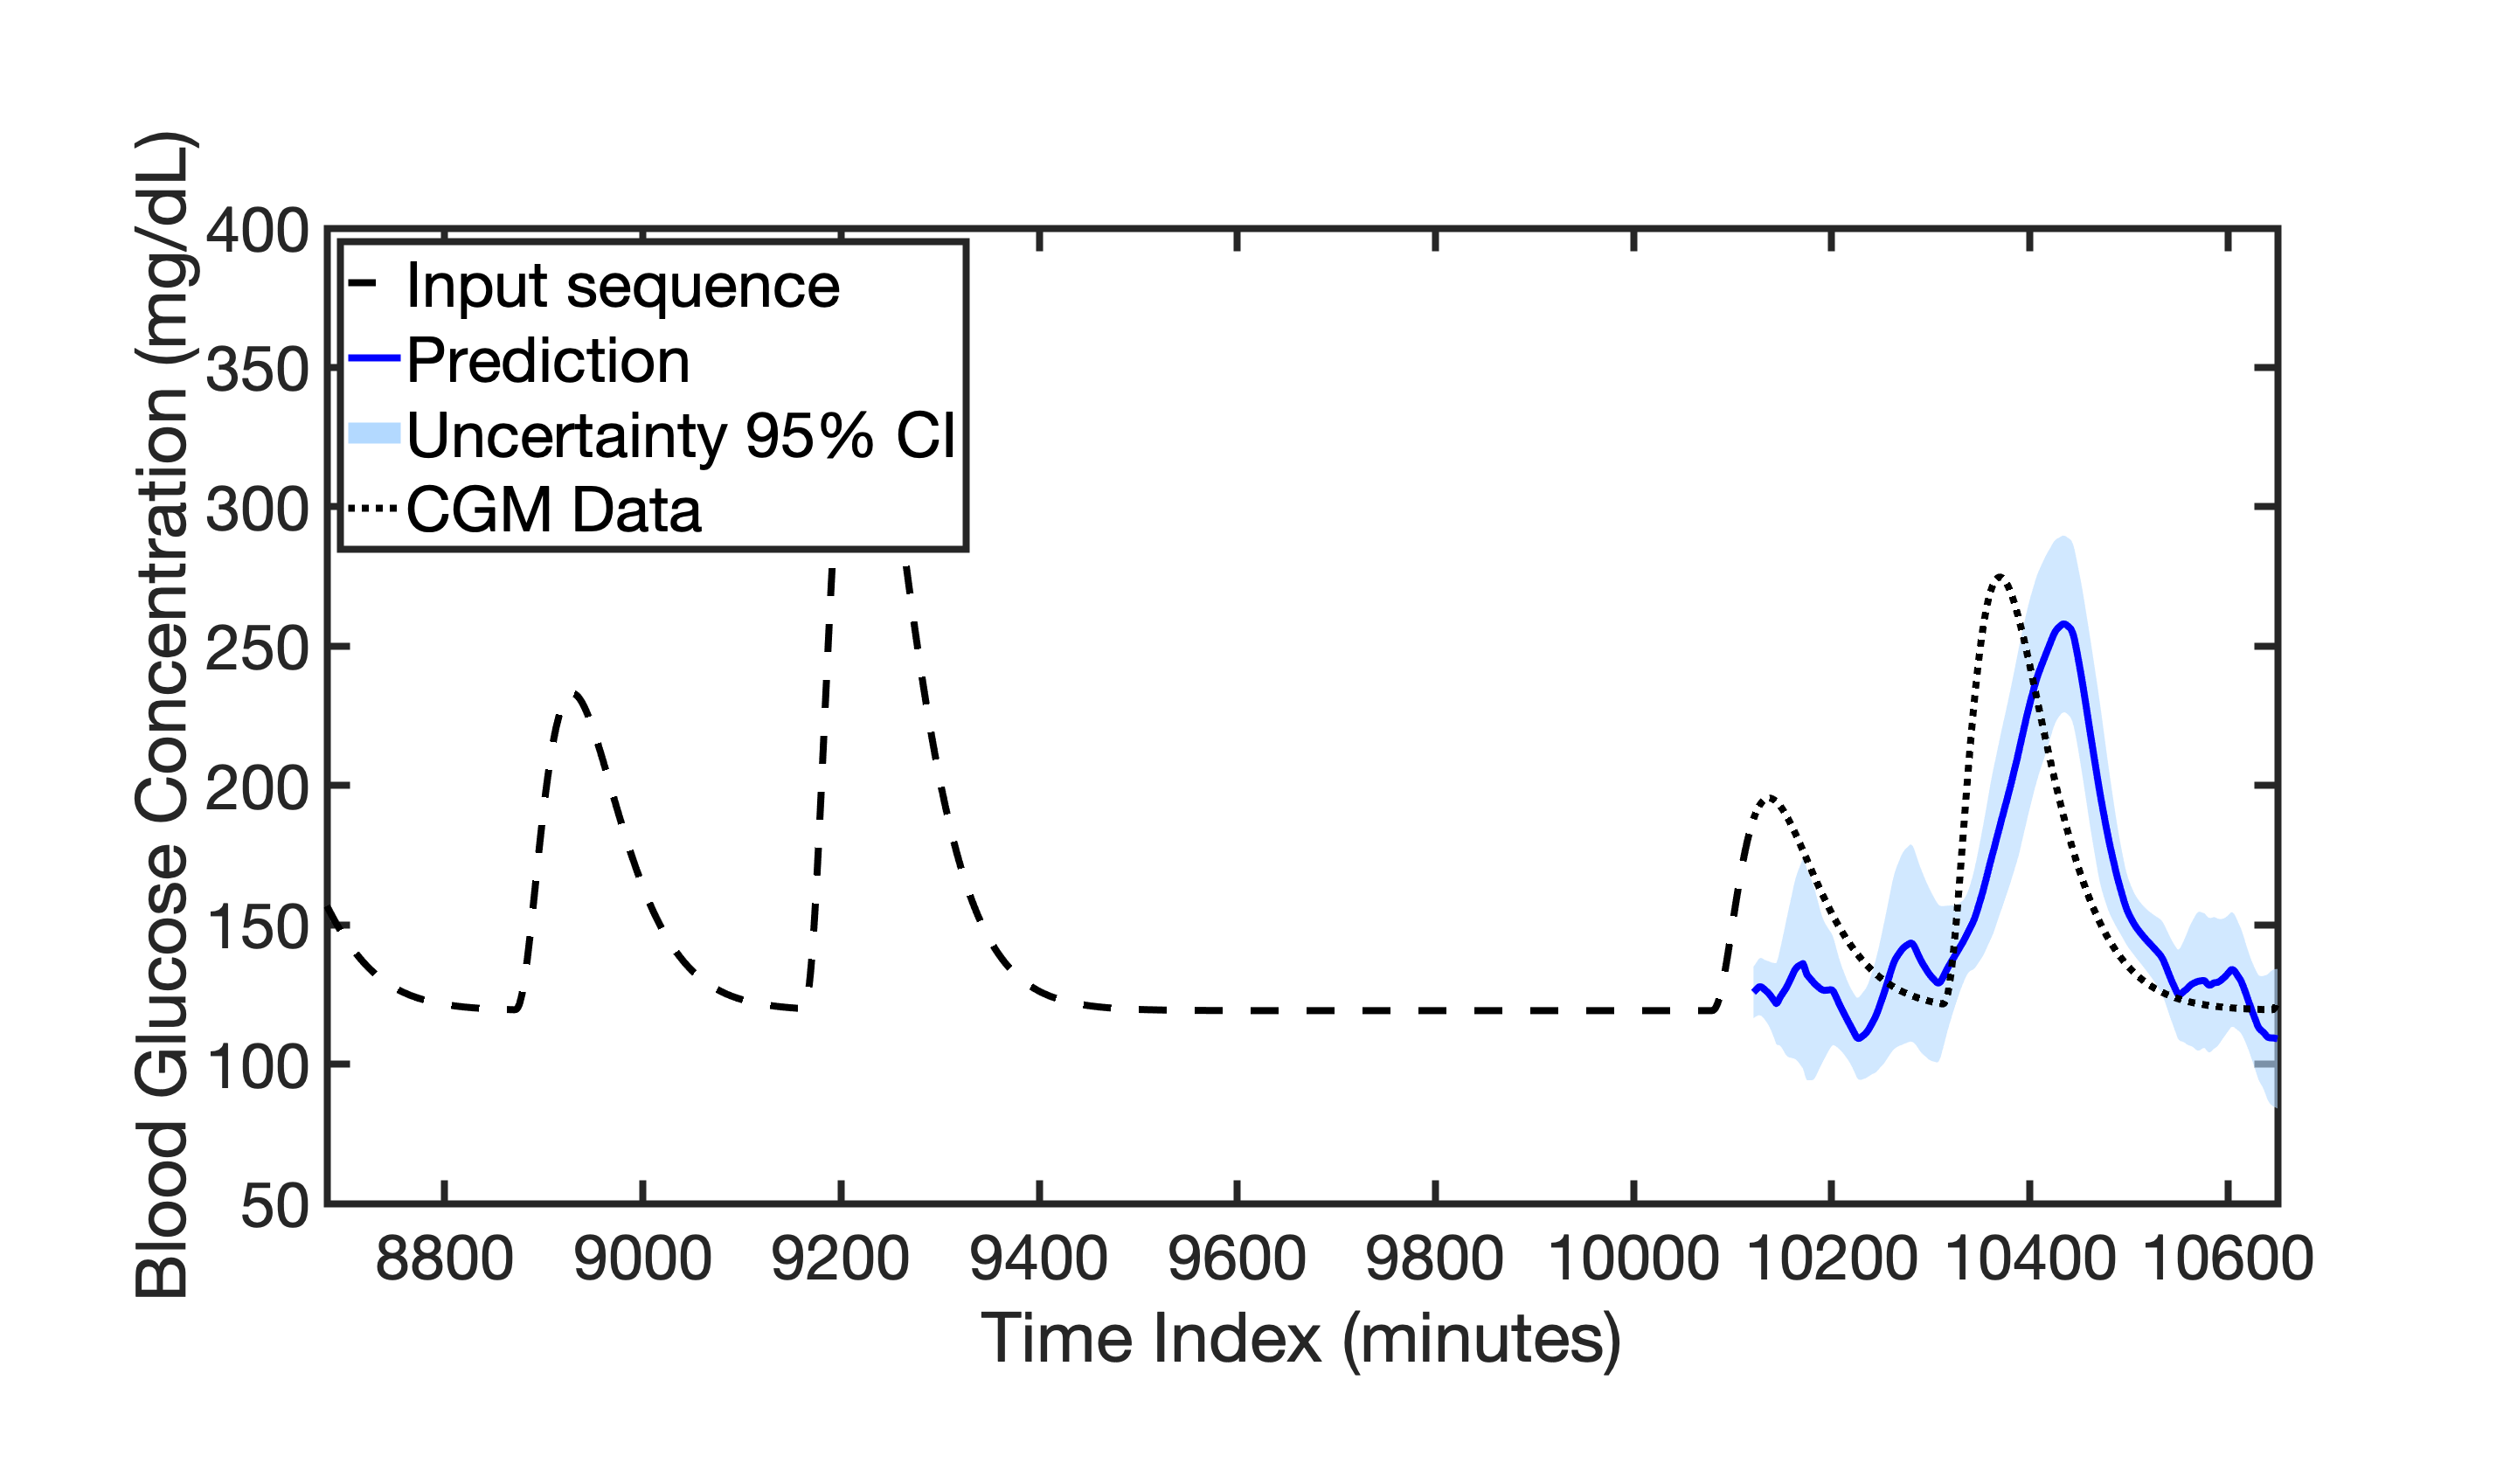
\includegraphics[width=\linewidth]{Figures/results/pred_pointB.png}
  \caption*{(e)}
\end{minipage}%
\hfill
\begin{minipage}[t]{0.33\textwidth}
  \centering
  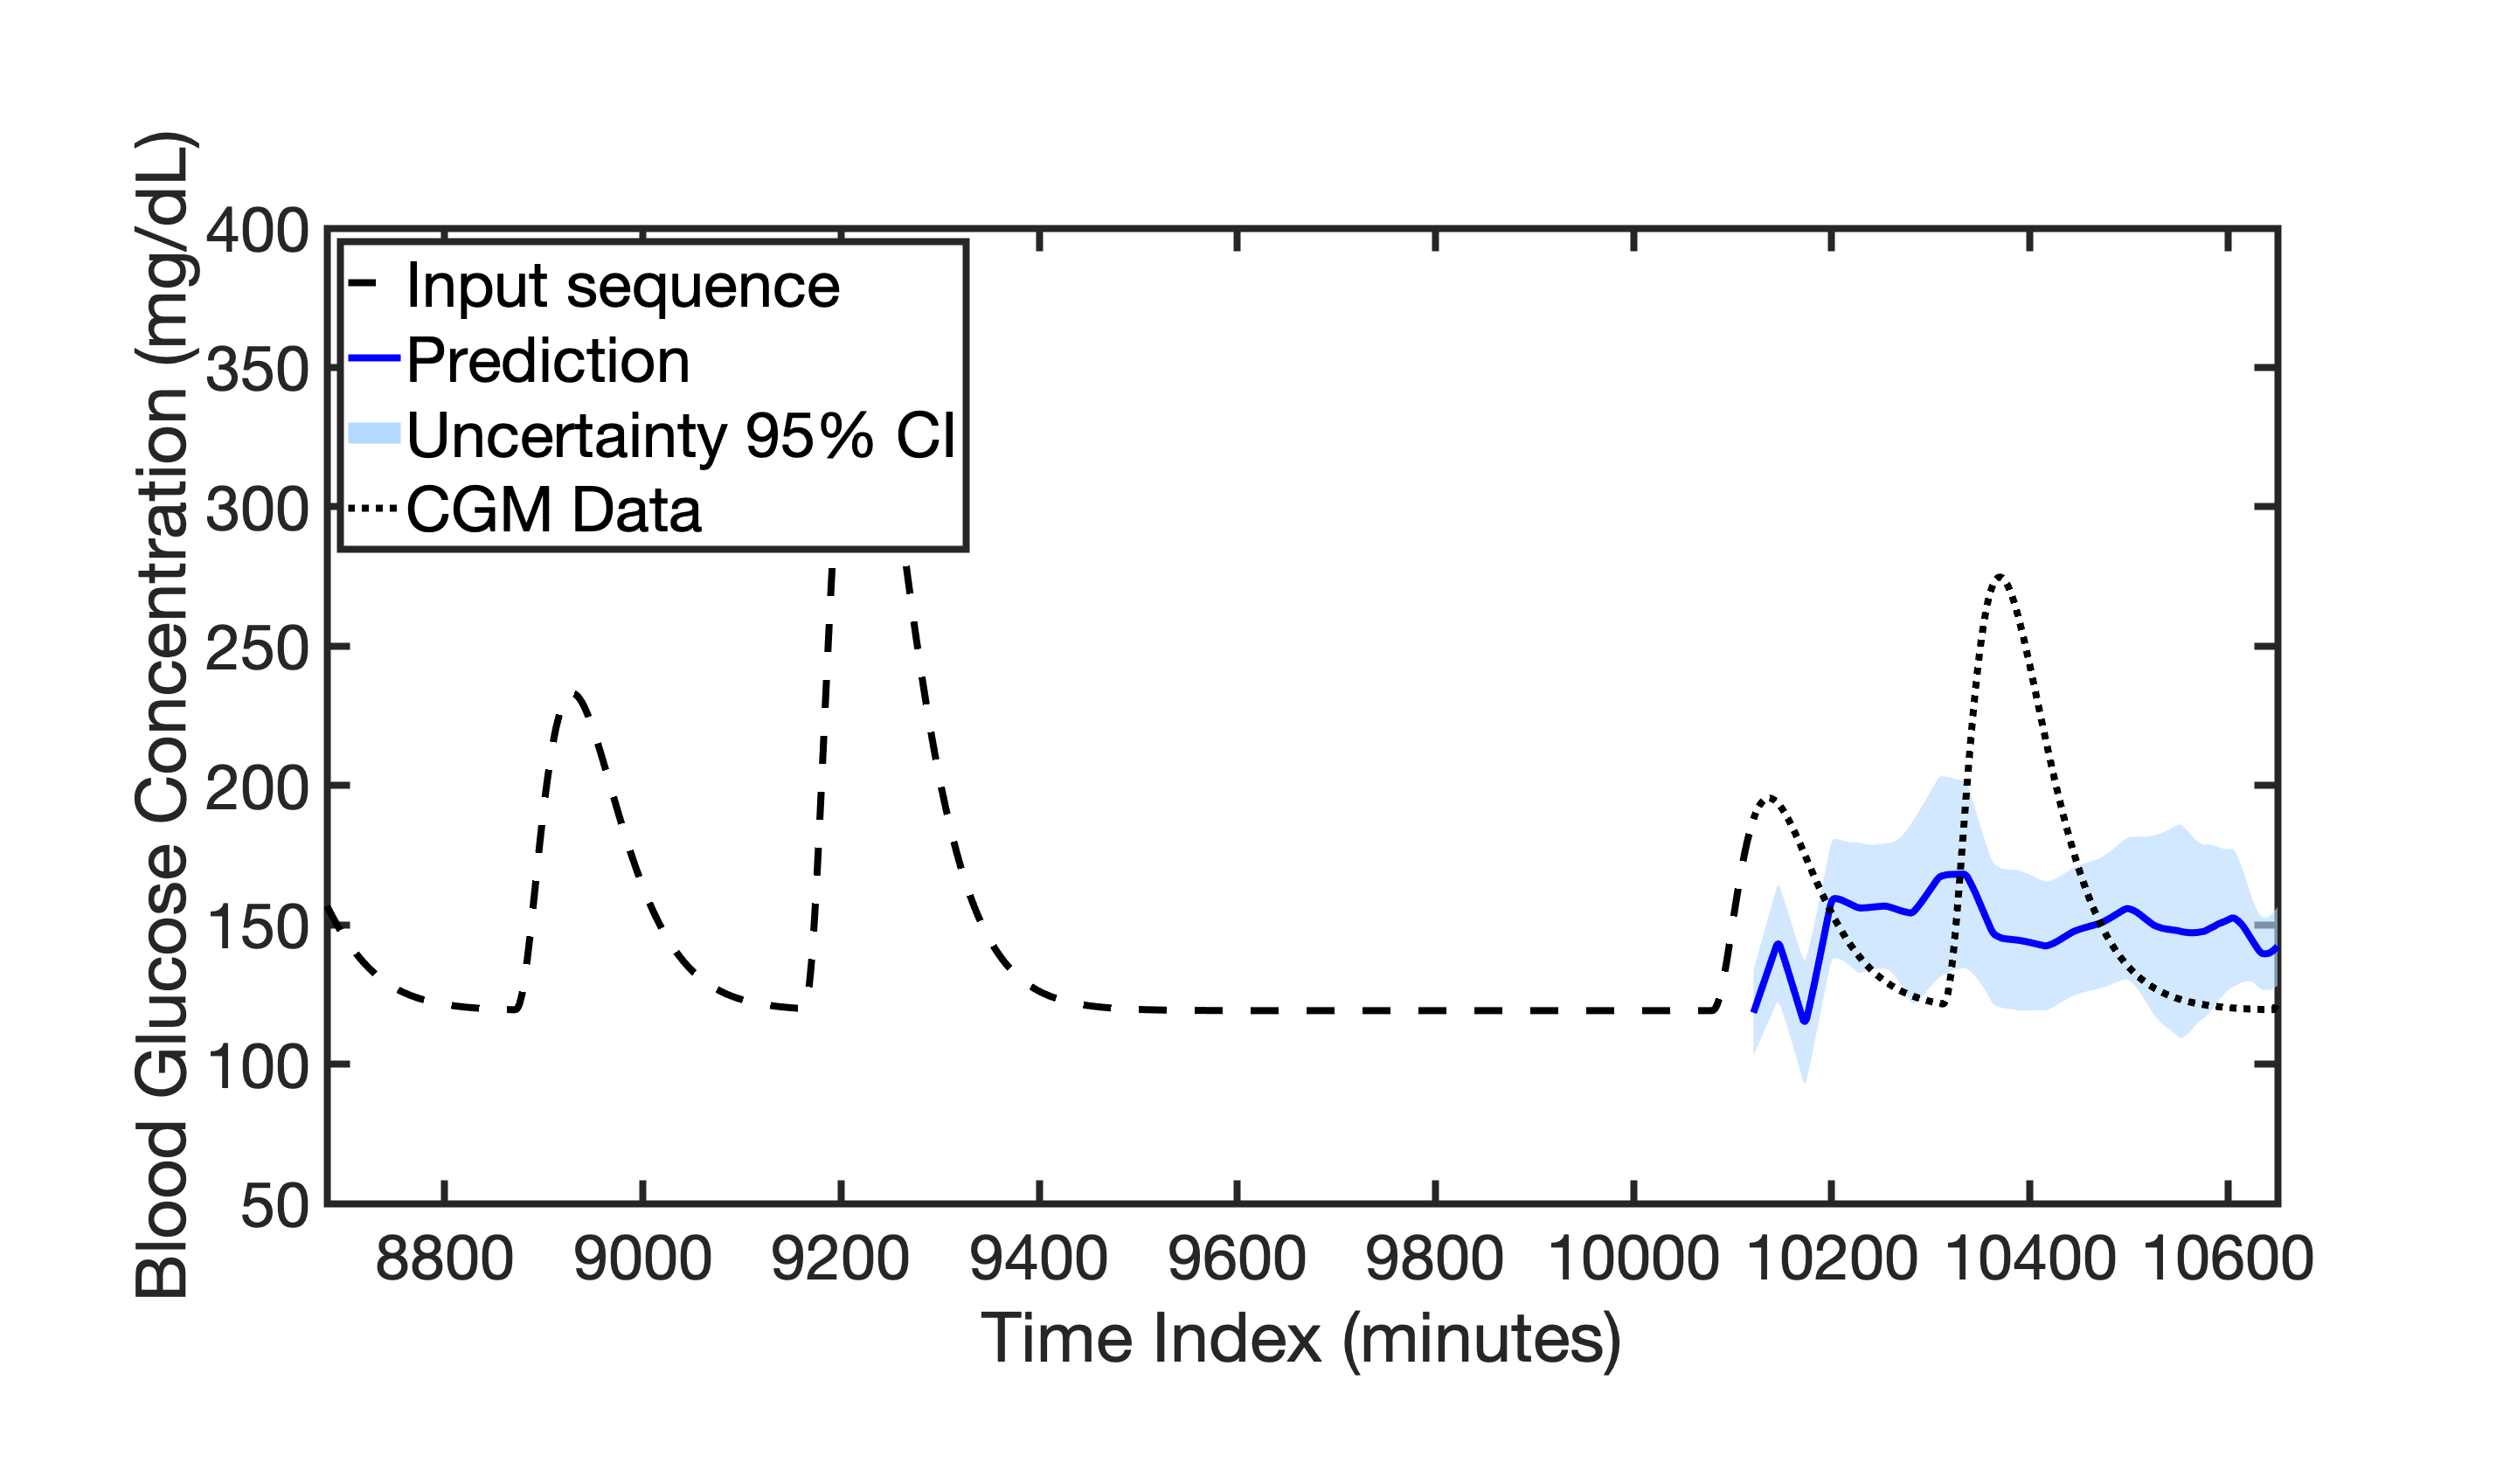
\includegraphics[width=\linewidth]{Figures/results/pred_pointC.png}
  \caption*{(f)}
\end{minipage}
\caption{(a) Training data fit for A, NLPD = 5.12, (b) Training data fit for B, NLPD = 5.15, (c) Training data fit for C, NLPD = 6.0, (d) Prediction for A, NLPD = 23.9, (e) Prediction for B, NLPD = 23.8, and (f) Prediction for C, NLPD = 25.15.}
\label{fig:trains}
\end{figure}

The predictive performance of these architectures can be illustrated with their NLPD values. NLPD is a probabilistic accuracy metric that evaluates predictions using both the mean error and the predicted uncertainty, penalizing models that are either wrong, over or under-confident. Its advantage is that it rewards well-calibrated uncertainty, making it better suited for risk-aware glucose forecasting and model selection.

\begin{equation}
\sigma_i^2 = \left(\sigma^{\mathrm{TCN}}_i\right)^2 + \left(\sigma^{\mathrm{data}}\right)^2
\label{eq:sigma_total}
\end{equation}

\begin{equation}
\mathrm{NLPD} =
\frac{1}{N}\sum_{i=1}^N
\left[
\frac{\left(\hat{G}^{\mathrm{TCN}}_i - \hat{G}^{\mathrm{data}}_i\right)^2}{\sigma_i^2}
+ \ln\!\left(\sigma_i^2\right)
\right]
\leq \mathrm{Tol}
\label{eq:nlpd}
\end{equation}

\noindent
Here, $\hat{G}^{\mathrm{TCN}}_i$ is the Bayesian TCN mean prediction of blood glucose at time $i$ and $\hat{G}^{\mathrm{data}}_i$ is the corresponding CGM-measured glucose value. The predictive uncertainty combines the model-derived standard deviation $\sigma^{\mathrm{TCN}}_i$ with the CGM sensor noise $\sigma^{\mathrm{data}}$.\\
These results show that (i) evidence provides a principled, quantitative criterion for selecting trustworthy TCN architectures, (ii) neither parameter count nor receptive field alone predicts performance, and (iii) the best-performing models arise from an intermediate design region that is sufficiently expressive to represent glucose excursions while avoiding unnecessary complexity that is not supported by the available data.



   \item 1D plausibility for input/output length. Conclusion => plausibility captures the data correlation

\autoref{fig:stride} evaluates the effect of the stride used to generate overlapping input--output windows from the CGM time series. The log-evidence peaks at an intermediate stride of 3 and decreases for both very small and large strides. A stride of 1 produces many highly redundant windows with limited additional information, while large strides reduce the number of training samples and degrade learnability. This result motivates using an intermediate stride 3 practical default, balancing statistical efficiency and dataset diversity.

\begin{figure}[H]
\centering

\begin{minipage}[t]{0.52\linewidth}\vspace{0pt}
    \centering
    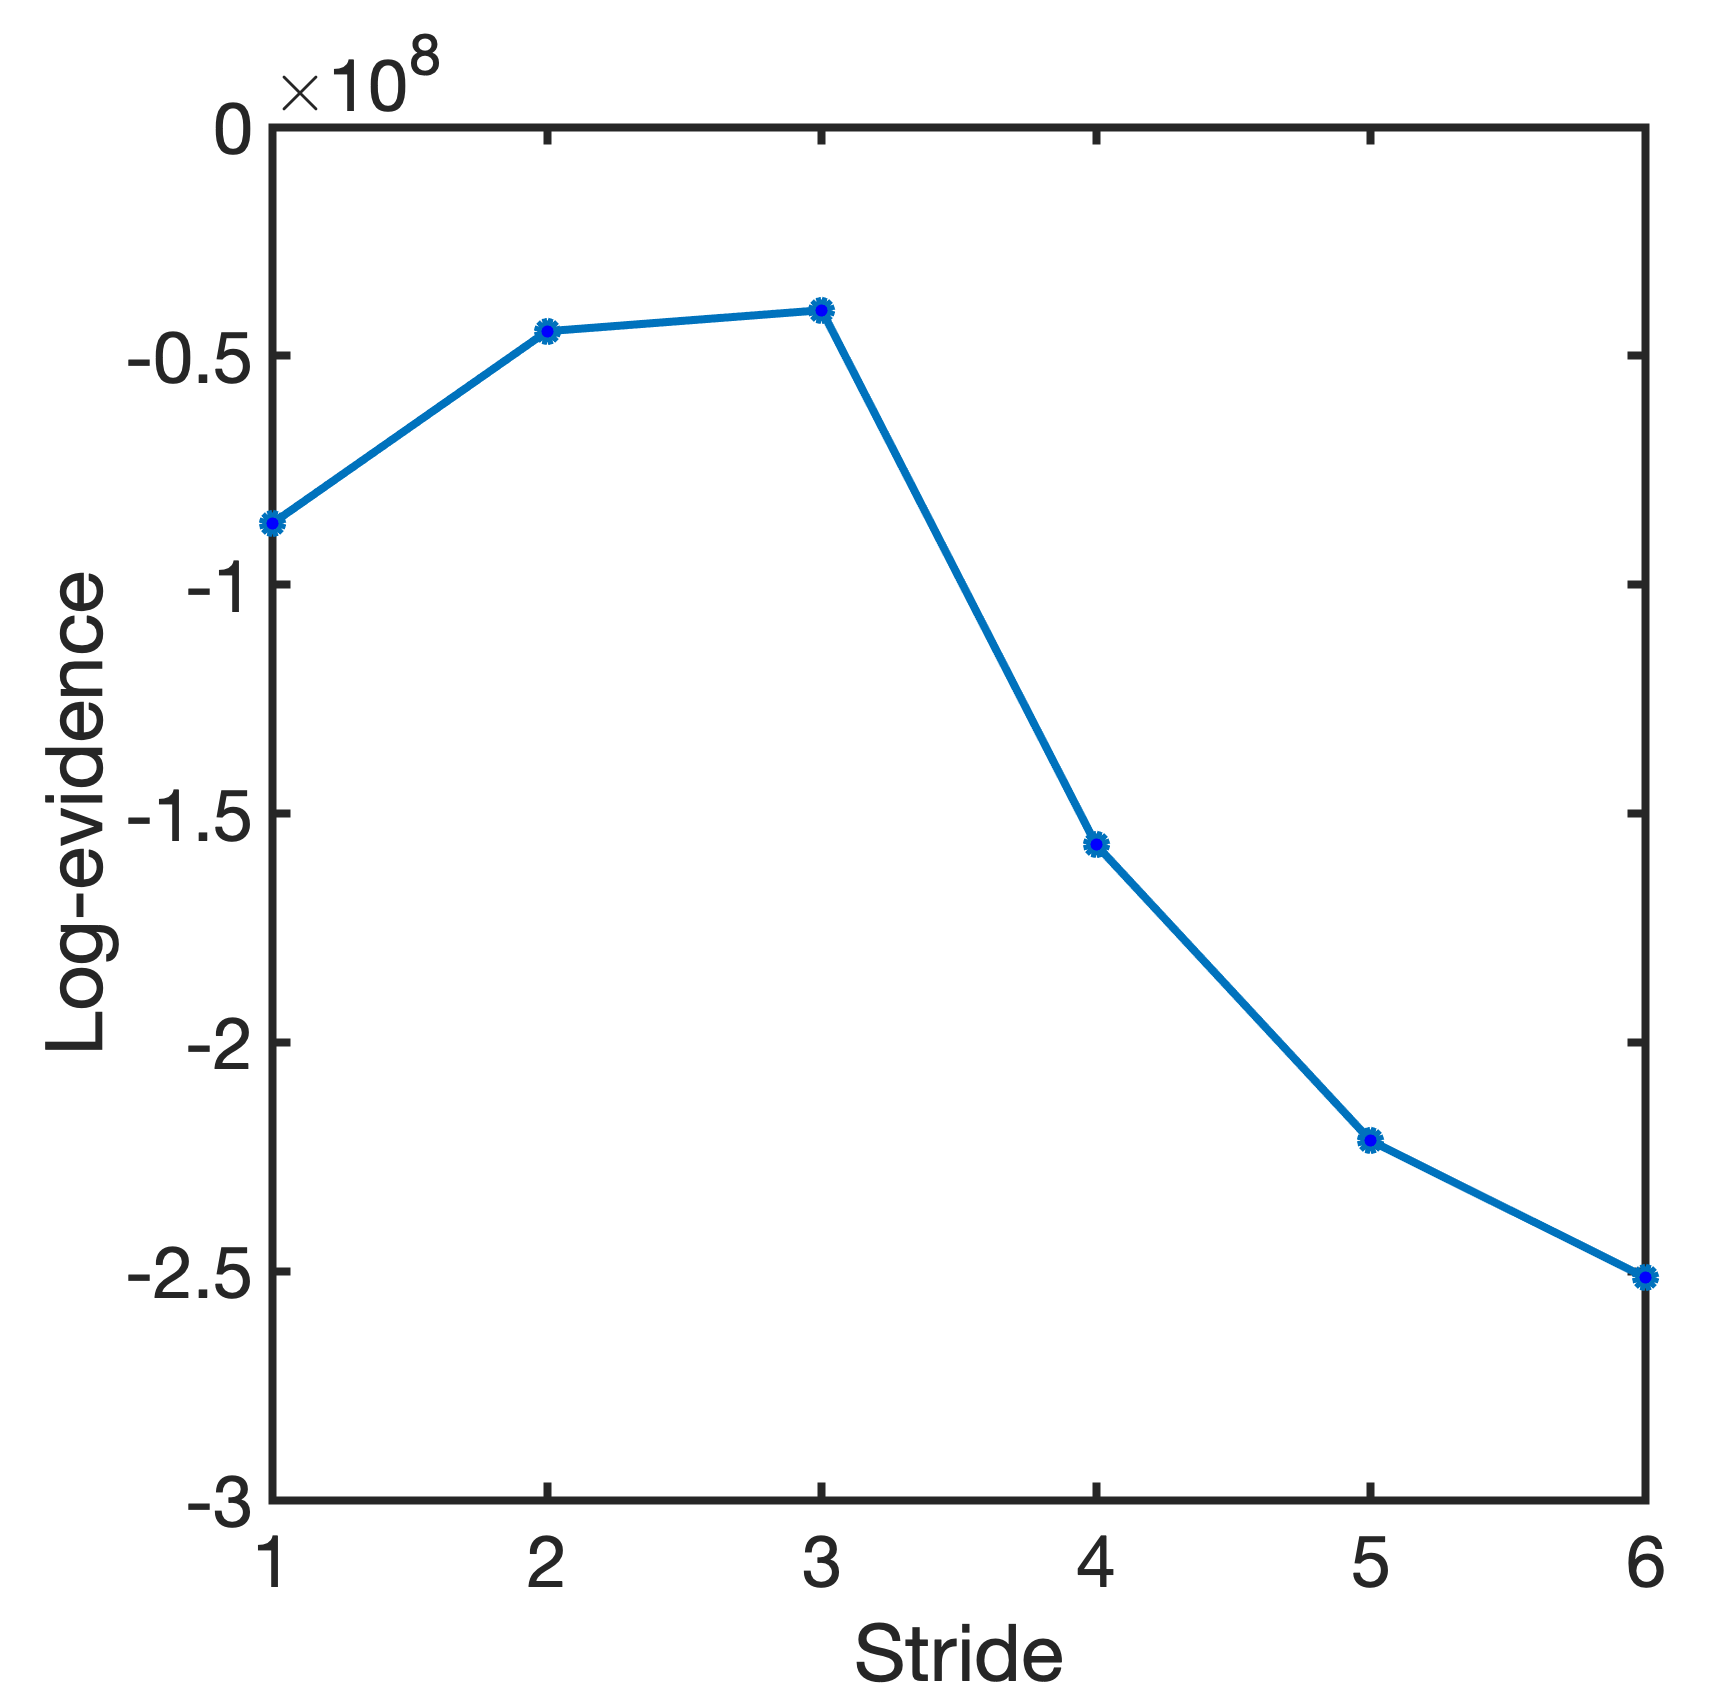
\includegraphics[width=\linewidth]{Figures/results/stride_vs_evid.png}
\end{minipage}
\begin{minipage}[t]{0.45\linewidth}\vspace{0pt}
    \centering
    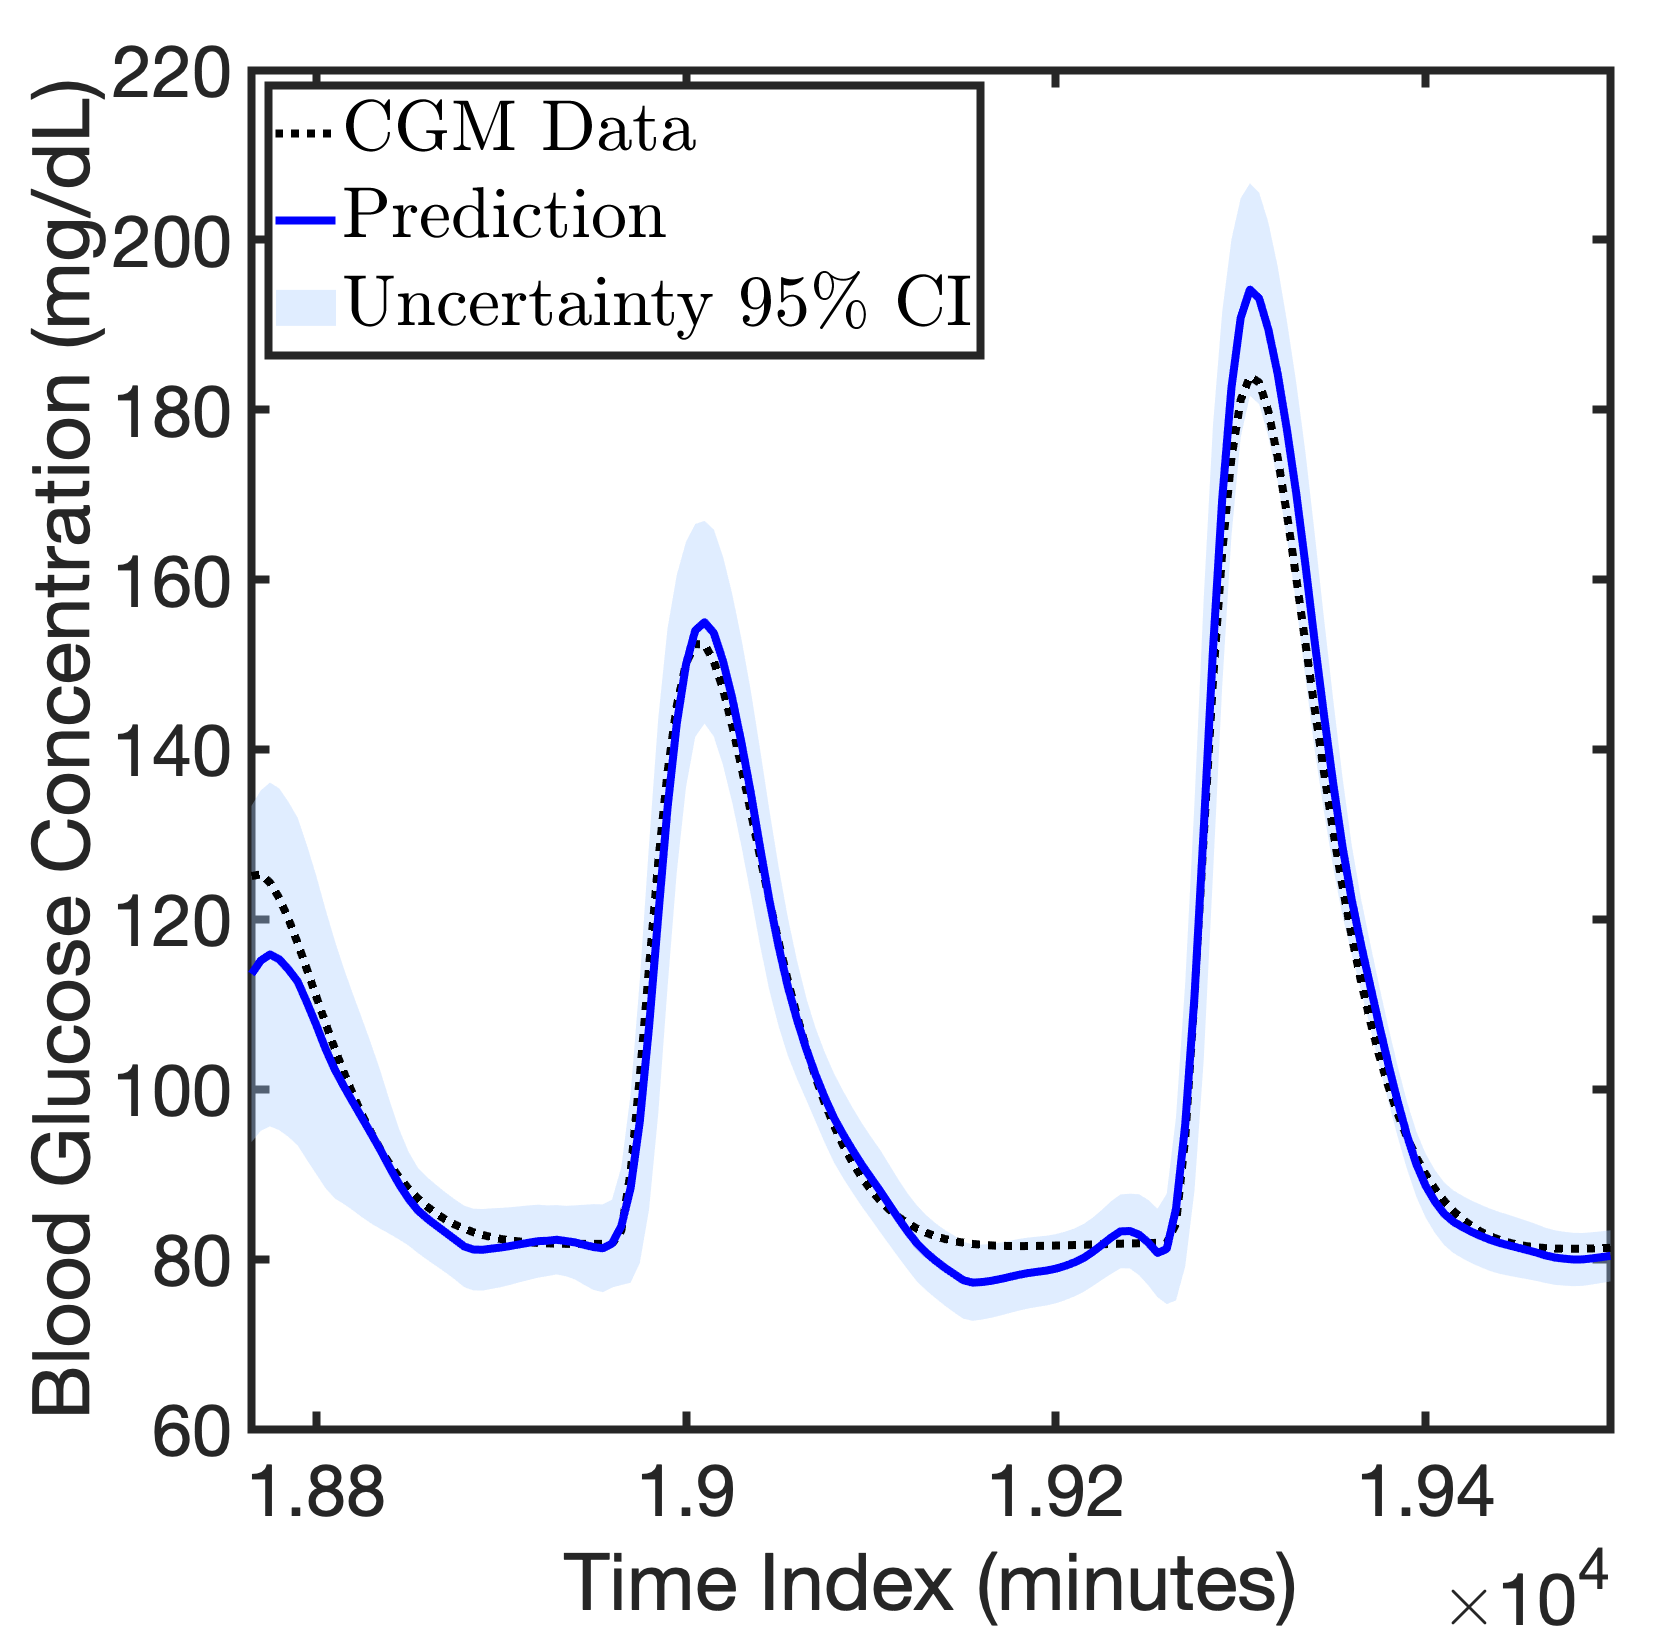
\includegraphics[width=\linewidth]{Figures/results/stride_3.png}
    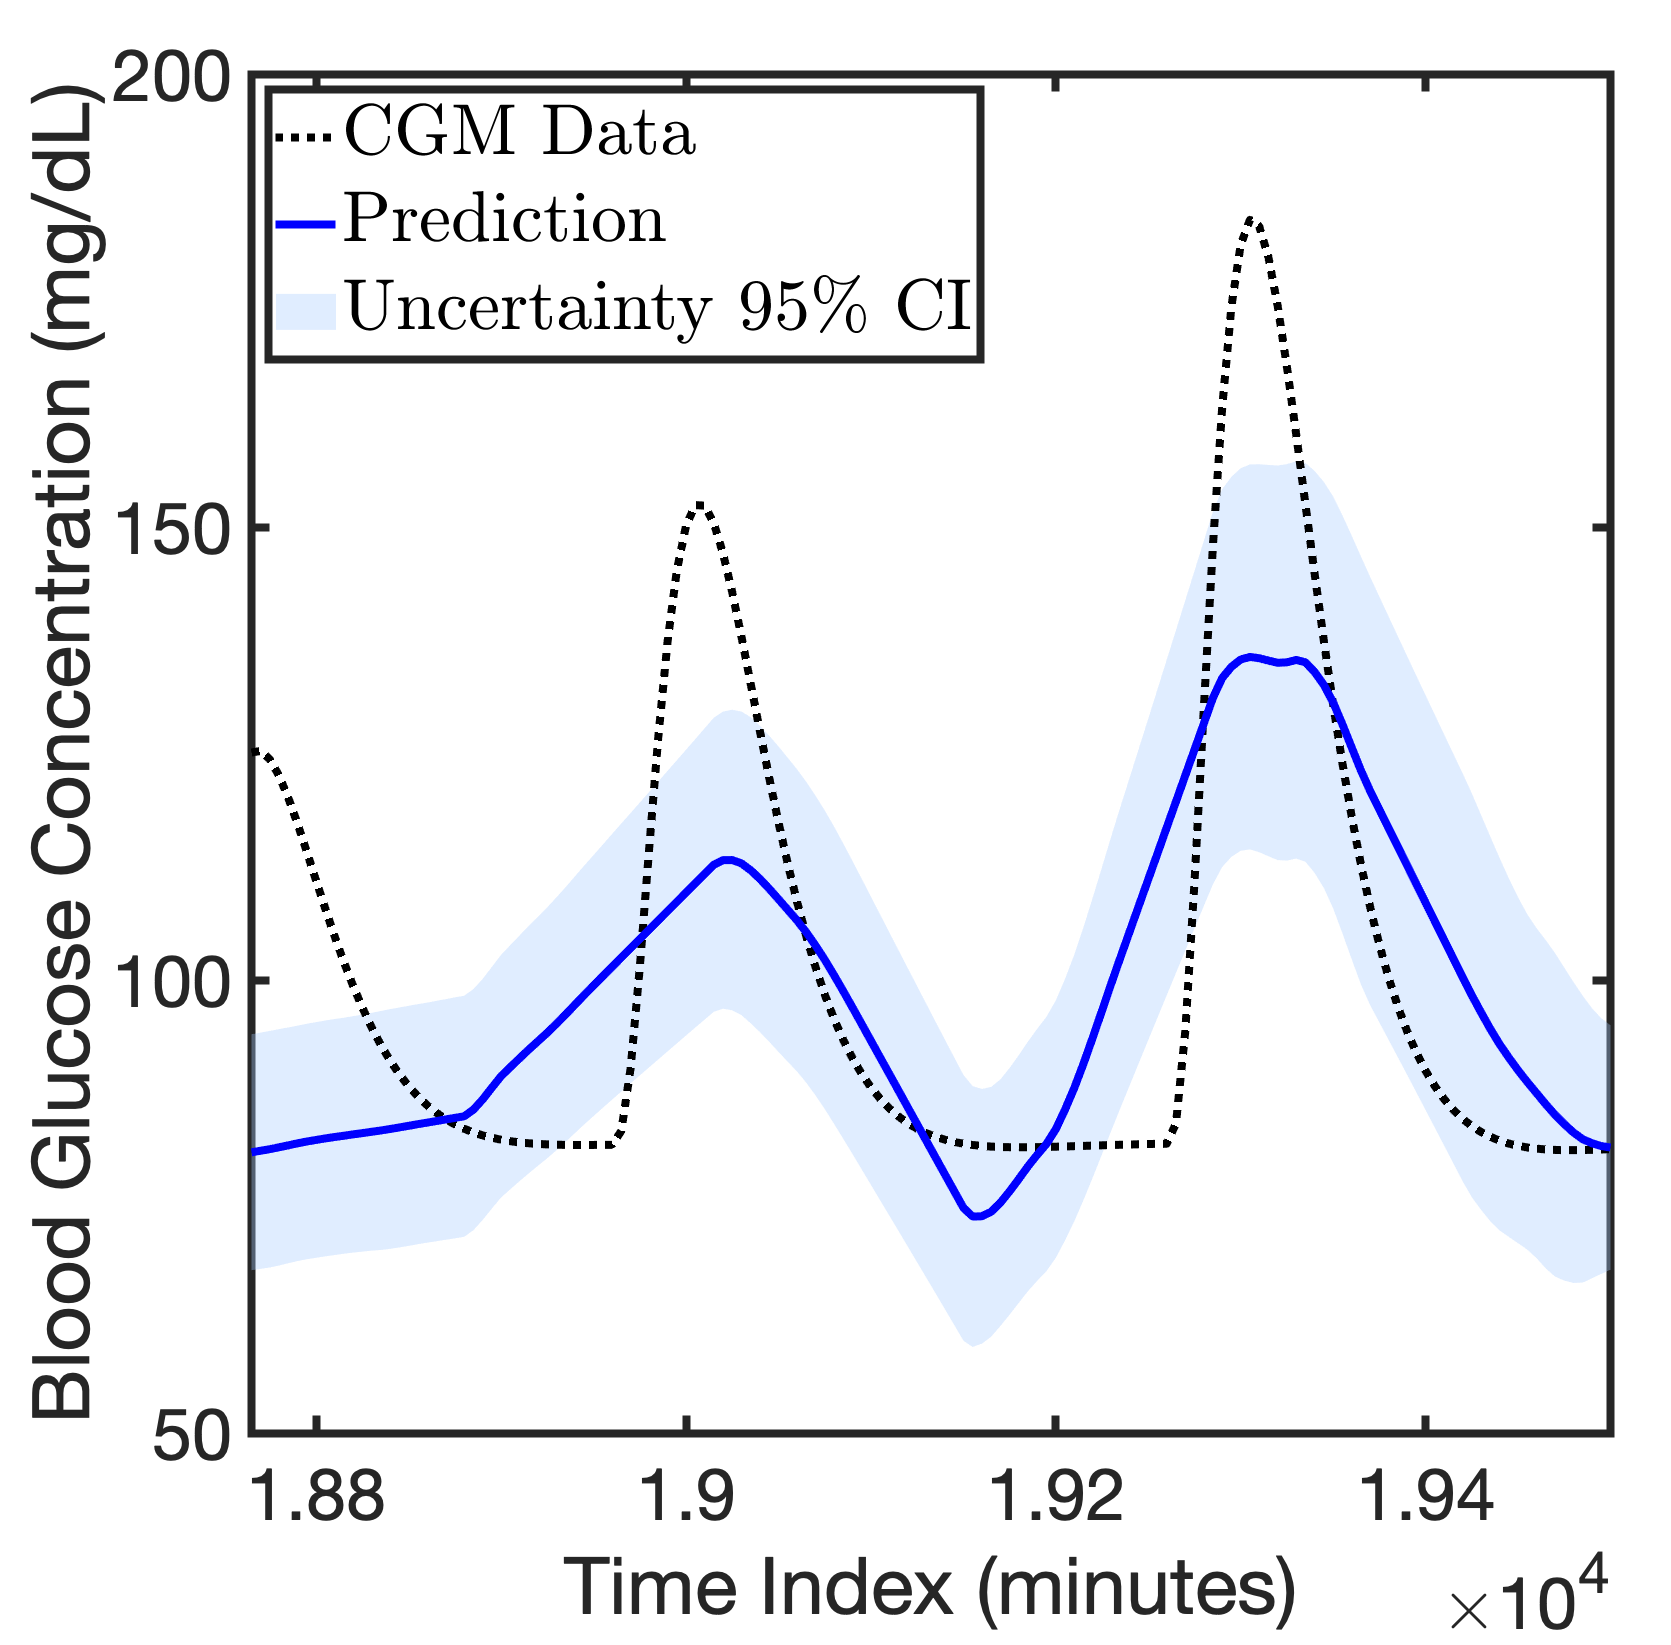
\includegraphics[width=\linewidth]{Figures/results/stride_6.png}
\end{minipage}
    \caption{Six strides values plotted against log-evidence (left). Prediction with stride of 3 (top right), Prediction with stride of 6 (bottom right)}
    \label{fig:stride}
\end{figure}

\autoref{fig:input_output} shows the log-evidence as a function of input history length and prediction horizon (output length). Evidence degrades strongly as the output horizon increases, indicating that longer-horizon forecasts are harder to support with the available data. To localize the high-evidence region, we first evaluate a coarse grid (200-min resolution) and then refine the region of interest with a fine grid (50-min resolution). 
\begin{figure}[H]
    \centering
    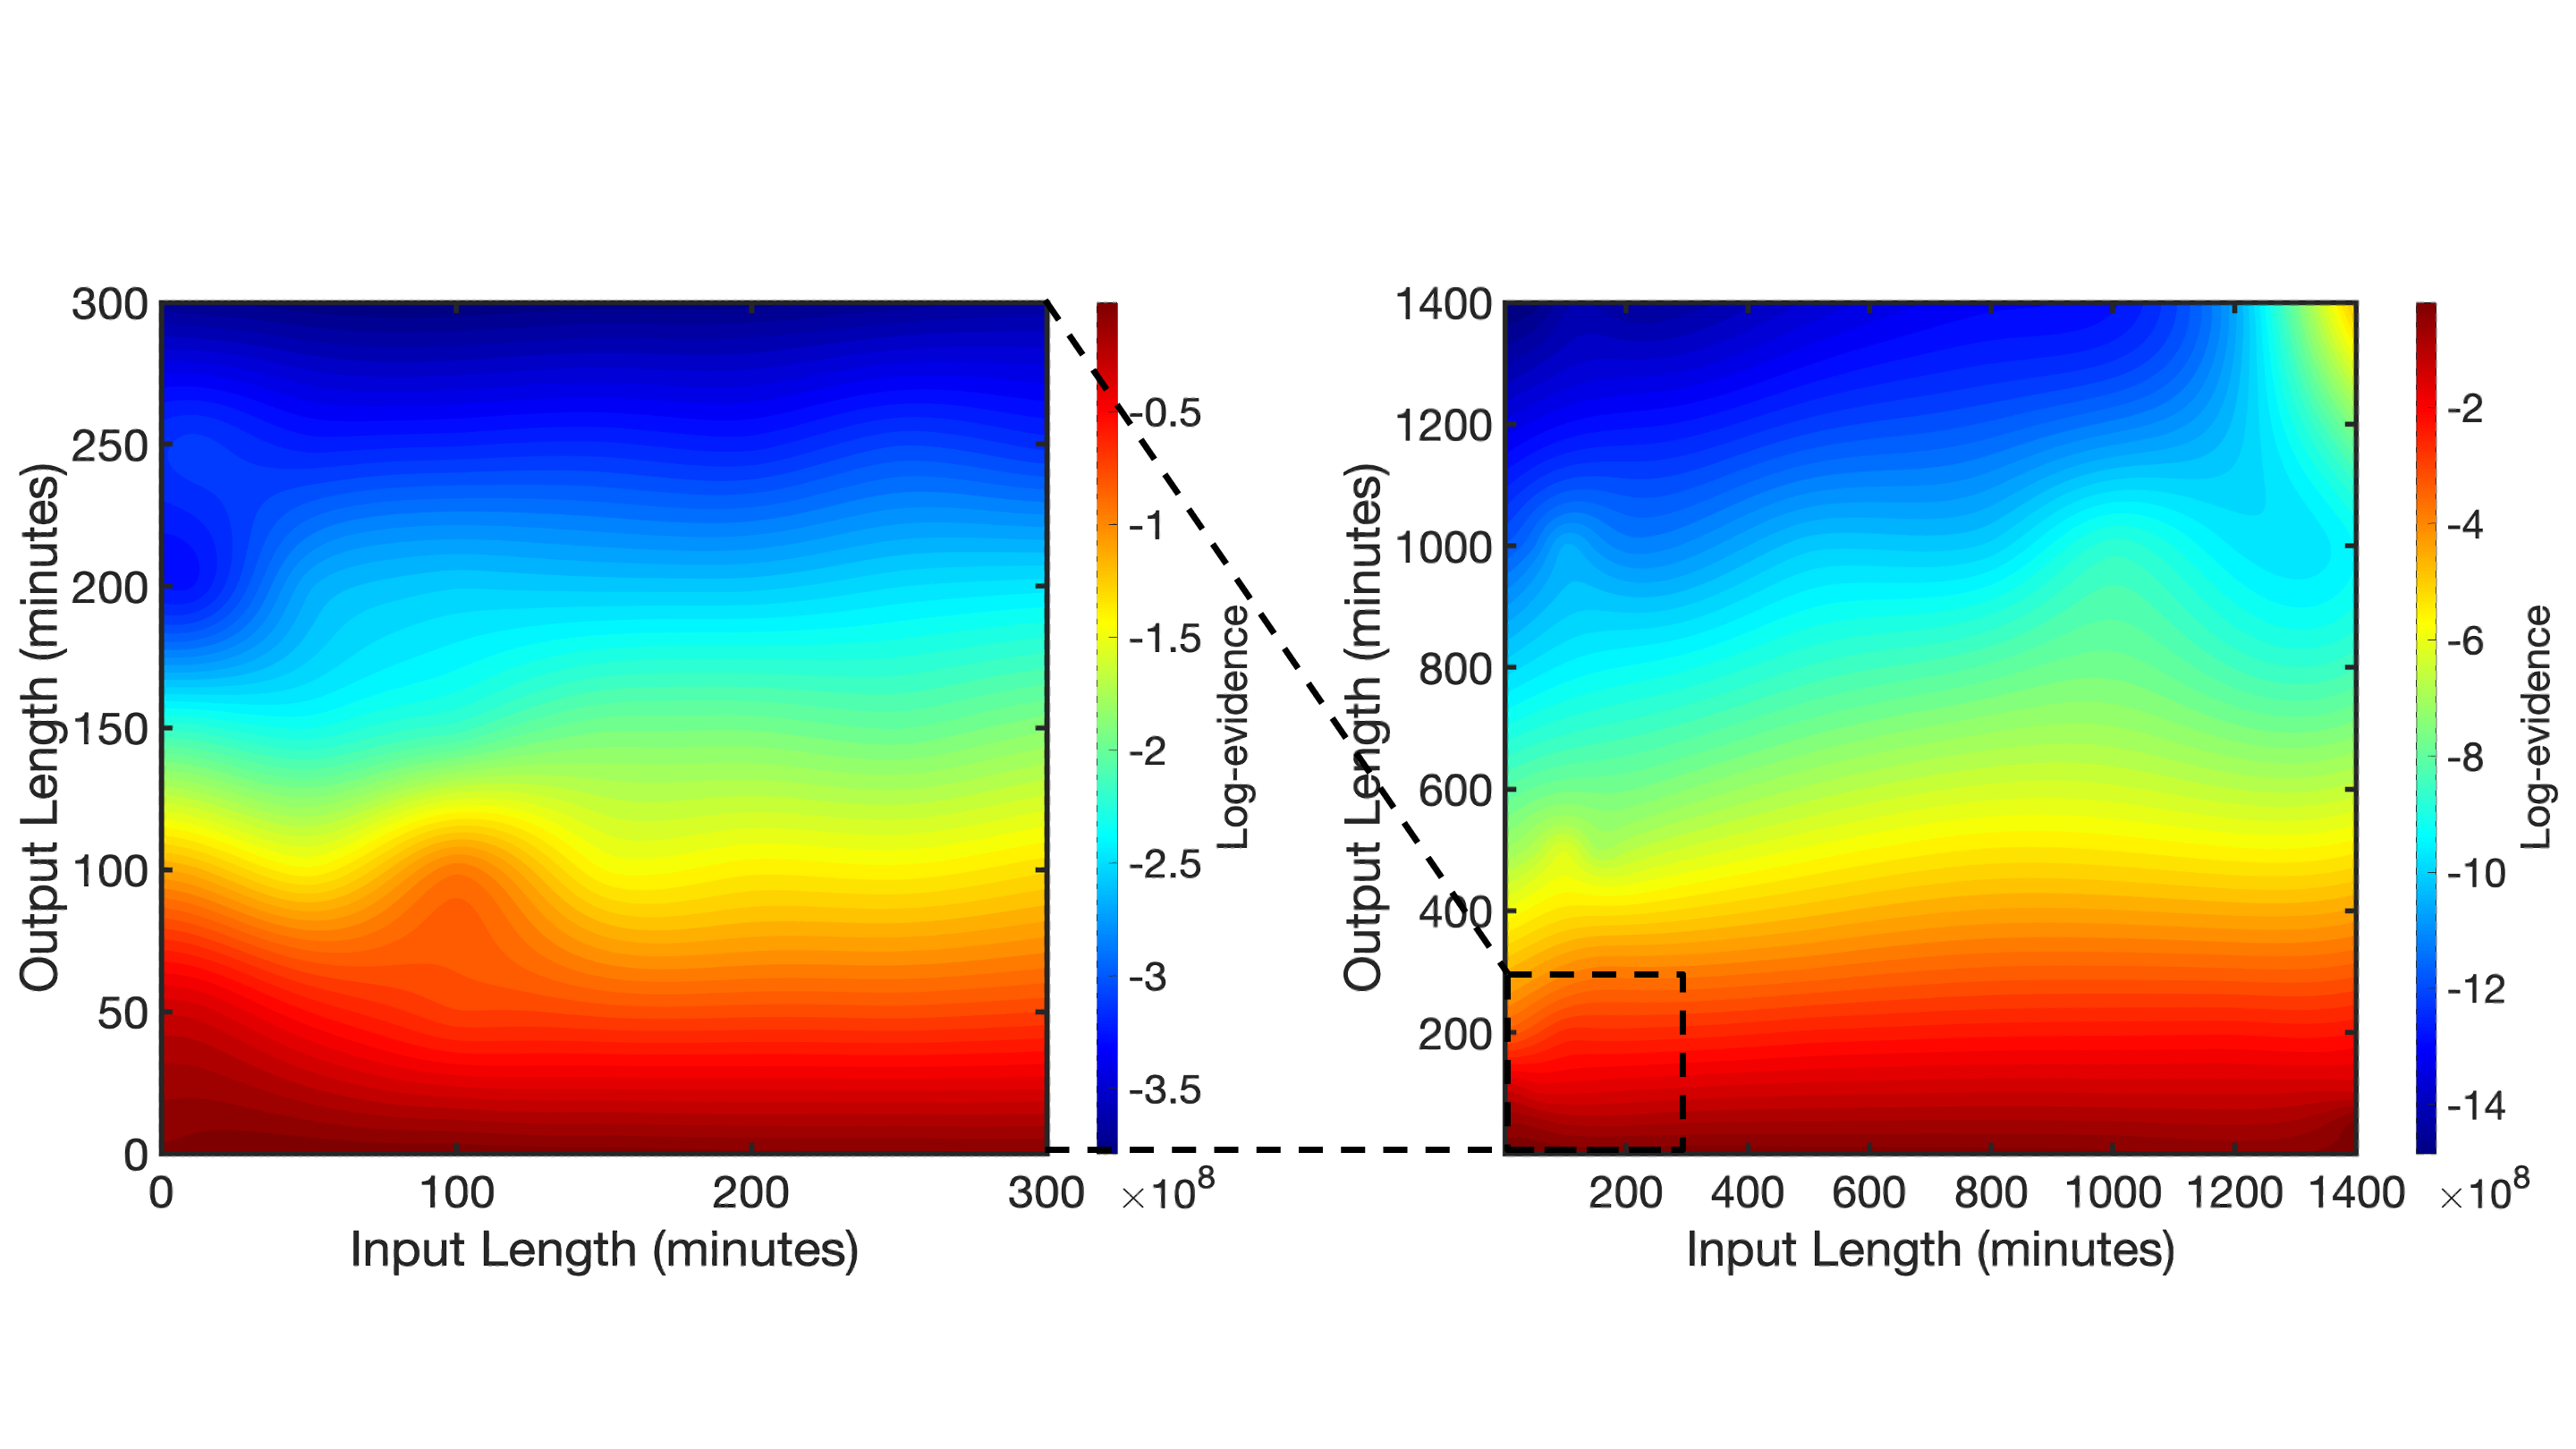
\includegraphics[width=\linewidth]{Figures/results/input_output.png}
\caption{Log-evidence surface as a function of input history length and prediction horizon (output length). The left panel shows the full sweep over 0-1400 minutes for both input and output lengths using a coarse grid with 200 min spacing. The red box highlights a region of interest. The right panel re-evaluates this 300 $\times$ 300 minutes region using a finer grid with 50 min spacing.}

    \label{fig:input_output}
\end{figure}

\end{itemize}




%++++++++++++++++++++++++++++++++++++++++++++++++++++++++++++++++++++++++
\subsection{B-TCN Model discovery using population-based diabetes/CGM data}\label{sec:opal_results}

\begin{itemize}
    \item Table of the 61 model and how they are determined based on RF + mention we stop prediction before meals

We construct a constrained pool of TCN architectures by enforcing receptive-field (RF) and dilation feasibility conditions, along with some calculative assumptions. The primary constraint is that the RF must cover at least one day of history to capture both diurnal and nocturnal glucose pattern:
\begin{equation}
1440 \le RF_n \le 2000 .
\label{eq:rf_constraint}
\end{equation}
To avoid ``holes'' in the dilated convolution coverage, we additionally require the no-holes condition
\begin{equation}
k \ge b ,
\label{eq:no_holes}
\end{equation}
where $k$ is the kernel size and $b$ is the dilation base. We restrict kernel sizes to $k \le 15$ and define the channel width per temporal block to start at 2 filters and grow up to a maximum of 512, using a doubling rule across temporal blocks (encoder--decoder) to maintain a structured increase in representational capacity \cite{ronneberger2015u} \cite{badrinarayanan2017segnet}.
Applying \eqref{eq:rf_constraint}--\eqref{eq:no_holes} together with these practical bounds yields a finite feasible design space of 61 candidate architectures for subsequent evidence-based screening and validation. During evaluation, prediction horizons are terminated 10 minutes before each annotated meal time to prevent contamination of the prediction horizon by imminent meal disturbances.
\noindent
Based on number of parameters, we can categorize the architectures into a total of 6 categories. 


\begin{footnotesize}
\setlength{\tabcolsep}{6pt}
\begin{longtable}{ccccccc}
\caption{TCN architectures for category 1}
\label{tab:cat1}\\
\toprule
\textbf{Category} & \textbf{ParamCount}& \textbf{ArchCount} & \textbf{\# Temporal Blocks} & \textbf{Starting \# filters} & \textbf{\# $(k, b)$ Pairs} \\
\midrule
\endfirsthead

\toprule
\textbf{Category} & \textbf{ParamCount}& \textbf{ArchCount} & \textbf{\# Temporal Blocks} & \textbf{\# filters $f$} & \textbf{\# $(k, b)$} \\
\midrule
\endhead

\endfoot

\bottomrule
\endlastfoot
1 & $\le$30k & 10 & [3, 4] & [2, 4] & 6 \\
2 & 30k-100k & 9 & [3, 4, 5, 6] & [2, 4, 8] & 9 \\
3 & 100k-400k & 10 & [3, 4, 5, 6] & [2, 4, 8, 16] & 10 \\
4 & 400k-1M & 11 & [3, 4, 5, 6, 7] & [2, 4, 8, 16, 32] & 11 \\
5 & 1M-5M & 11 & [3, 4, 5, 6, 7] & [4, 8, 16, 32, 64] & 11  \\
6 & $\ge$5M & 10 & [3, 4, 5, 6, 7] & [8, 16, 32, 64, 128] & 10 \\
\end{longtable}
\end{footnotesize}


Tables [2-4] depicts all architectures from the first 3 categories respectively. 


\begin{footnotesize}
\setlength{\tabcolsep}{6pt}
\begin{longtable}{ccccccc}
\caption{TCN architectures for category 1}
\label{tab:cat1}\\
\toprule
\textbf{ArchName} & \textbf{ParamCount} & \textbf{Layers} & \textbf{Dilation} & \textbf{Filter Size} & \textbf{Encoder Channels} & \textbf{Decoder Channels} \\
\midrule
\endfirsthead

\toprule
\textbf{ArchName} & \textbf{ParamCount} & \textbf{Layers} & \textbf{Dilation} & \textbf{Filter Size} & \textbf{Encoder Channels} & \textbf{Decoder Channels} \\
\midrule
\endhead

\endfoot

\bottomrule
\endlastfoot

$Cat_1Arch_1$ & 2756  & 3 & 9 & 9  & $[2,4,8]$        & $[8,4,2]$ \\
$Cat_1Arch_2$ & 3356  & 3 & 8 & 11 & $[2,4,8]$        & $[8,4,2]$ \\
$Cat_1Arch_3$ & 3356  & 3 & 9 & 11 & $[2,4,8]$        & $[8,4,2]$ \\
$Cat_1Arch_4$ & 3956  & 3 & 8 & 13 & $[2,4,8]$        & $[8,4,2]$ \\
$Cat_1Arch_5$ & 8492  & 4 & 5 & 7  & $[2,4,8,16]$     & $[16,8,4,2]$ \\
$Cat_1Arch_6$ & 10696 & 3 & 9 & 9  & $[4,8,16]$       & $[16,8,4]$ \\
$Cat_1Arch_7$ & 13048 & 3 & 8 & 11 & $[4,8,16]$       & $[16,8,4]$ \\
$Cat_1Arch_8$ & 13048 & 3 & 9 & 11 & $[4,8,16]$       & $[16,8,4]$ \\
$Cat_1Arch_9$ & 13276 & 4 & 4 & 11 & $[2,4,8,16]$     & $[16,8,4,2]$ \\
$Cat_1Arch_{10}$ & 15400 & 3 & 8 & 13 & $[4,8,16]$     & $[16,8,4]$ \\
\end{longtable}
\end{footnotesize}



\begin{footnotesize}
\setlength{\tabcolsep}{6pt}
\begin{longtable}{ccccccc}
\caption{TCN architectures for category 2}
\label{tab:cat2}\\
\toprule
\textbf{ArchName} & \textbf{ParamCount} & \textbf{Layers} & \textbf{Dilation} & \textbf{Filter Size} & \textbf{Encoder Channels} & \textbf{Decoder Channels} \\
\midrule
\endfirsthead

\toprule
\textbf{ArchName} & \textbf{ParamCount} & \textbf{Layers} & \textbf{Dilation} & \textbf{Filter Size} & \textbf{Encoder Channels} & \textbf{Decoder Channels} \\
\midrule
\endhead

\endfoot

\bottomrule
\endlastfoot
$Cat_2Arch_1$ & 33560 & 4 & 5 & 7  & [4, 8, 16, 32]        & [32, 16, 8, 4]\\
$Cat_2Arch_2$ & 33708 & 5 & 3 & 7  & [2, 4, 8, 16, 32]     & [32, 16, 8, 4, 2] \\
$Cat_2Arch_3$ & 42128 & 3 & 9 & 9  & [8, 16, 32]           & [32, 16, 8]\\
$Cat_2Arch_4$ & 43268 & 5 & 3 & 9  & [2, 4, 8, 16, 32]     & [32, 16, 8, 4, 2] \\
$Cat_2Arch_5$ & 51440 & 3 & 8 & 11 & [8, 16, 32]           & [32, 16, 8] \\
$Cat_2Arch_6$ & 51440 & 3 & 9 & 11 & [8, 16, 32]           & [32, 16, 8]\\
$Cat_2Arch_7$ & 52600 & 4 & 4 & 11 & [4, 8, 16, 32]        & [32, 16, 8, 4] \\
$Cat_2Arch_8$ & 57852 & 6 & 3 & 3  & [2, 4, 8, 16, 32, 64] & [64, 32, 16, 8, 4, 2] \\
$Cat_2Arch_9$ & 60752 & 3 & 8 & 13 & [8, 16, 32]           & [32, 16, 8]\\
\end{longtable}
\end{footnotesize}

\begin{footnotesize}
\setlength{\tabcolsep}{6pt}
\begin{longtable}{ccccccc}
\caption{TCN architectures for category 3}
\label{tab:cat3}\\
\toprule
\textbf{ArchName} & \textbf{ParamCount} & \textbf{Layers} & \textbf{Dilation} & \textbf{Filter Size} & \textbf{Encoder Channels} & \textbf{Decoder Channels} \\
\midrule
\endfirsthead

\toprule
\textbf{ArchName} & \textbf{ParamCount} & \textbf{Layers} & \textbf{Dilation} & \textbf{Filter Size} & \textbf{Encoder Channels} & \textbf{Decoder Channels} \\
\midrule
\endhead

\endfoot

\bottomrule
\endlastfoot

$Cat_3Arch_1$ & 133424 & 4 & 5 & 7  & [8, 16, 32, 64]          & [64, 32, 16, 8]  \\
$Cat_3Arch_2$ & 134168 & 5 & 3 & 7  & [4, 8, 16, 32, 64]       & [64, 32, 16, 8, 4] \\
$Cat_3Arch_3$ & 167200 & 3 & 9 & 9  & [16, 32, 64]             & [64, 32, 16]\\
$Cat_3Arch_4$ & 172360 & 5 & 3 & 9  & [4, 8, 16, 32, 64]       & [64, 32, 16, 8, 4] \\
$Cat_3Arch_5$ & 204256 & 3 & 8 & 11 & [16, 32, 64]             & [64, 32, 16] \\
$Cat_3Arch_6$ & 204256 & 3 & 9 & 11 & [16, 32, 64]             & [64, 32, 16]\\
$Cat_3Arch_7$ & 209392 & 4 & 4 & 11 & [8, 16, 32, 64]          & [64, 32, 16, 8] \\
$Cat_3Arch_8$ & 230328 & 6 & 3 & 3  & [4, 8, 16, 32, 64, 128]  & [128, 64, 32, 16, 8, 4]\\
$Cat_3Arch_9$ & 241312 & 3 & 8 & 13 & [16, 32, 64]             & [64, 32, 16] \\
$Cat_3Arch_{10}$ & 249012 & 6 & 2 & 13 & [2, 4, 8, 16, 32, 64]  & [64, 32, 16, 8, 4, 2]\\
\end{longtable}
\end{footnotesize}




    \item Population based data description + cross-validation folds + Figure

Population-based type-1 diabetes (T1D) trajectories were generated using the FDA-approved UVA/Padova T1D simulator environment \cite{man2014uva}. We simulated 10 adult virtual subjects under the simulator’s default physiological settings and three meals per day. For each subject, the resulting time series included CGM glucose along with the corresponding exogenous inputs (meal/carbohydrate events and insulin delivery). The 10 patients were categorized into 5 folds with 8 patients in training set and rest 2 patients in the validation set as summarized in Table~\ref{tab:cv_folds}. The primary training configuration with the training set used an output length of $285$ minutes, chosen as the minimum inter-meal gap in the simulated scenarios so that each prediction horizon remains within a single inter-meal interval. All the input-output sequence pair with any meal in the prediction horizon was discarded. For the validation folds, models were trained on three days of data from the two leave-out subjects and validated on a separate day using a shorter prediction horizon (input: one day, output: $60$ minutes). For the training in each fold, the posterior from the initial training was used as the prior in the leave-out validation training. During evaluation, predictions were truncated to end $10$ minutes before each scheduled meal time to avoid scoring across meal onsets.


\begin{table}[H]
\centering
\caption{Patient-wise 5-fold cross-validation splits for the 10 adult virtual subjects.}
\label{tab:cv_folds}
\begin{tabular}{c l l}
\hline
\textbf{Fold} & \textbf{Training patients} & \textbf{Validation patients} \\
\hline
1 & Adults [1--8] & Adults [9, 10] \\
2 & Adults [1--5, 8--10] & Adults [6, 7] \\
3 & Adults [3--10] & Adults [1, 2] \\
4 & Adults [1, 2, 5--10] & Adults [3, 4] \\
5 & Adults [1--4, 6, 7, 9, 10] & Adults [5, 8] \\
\hline
\end{tabular}
\end{table}



\begin{figure}[H]
\centering
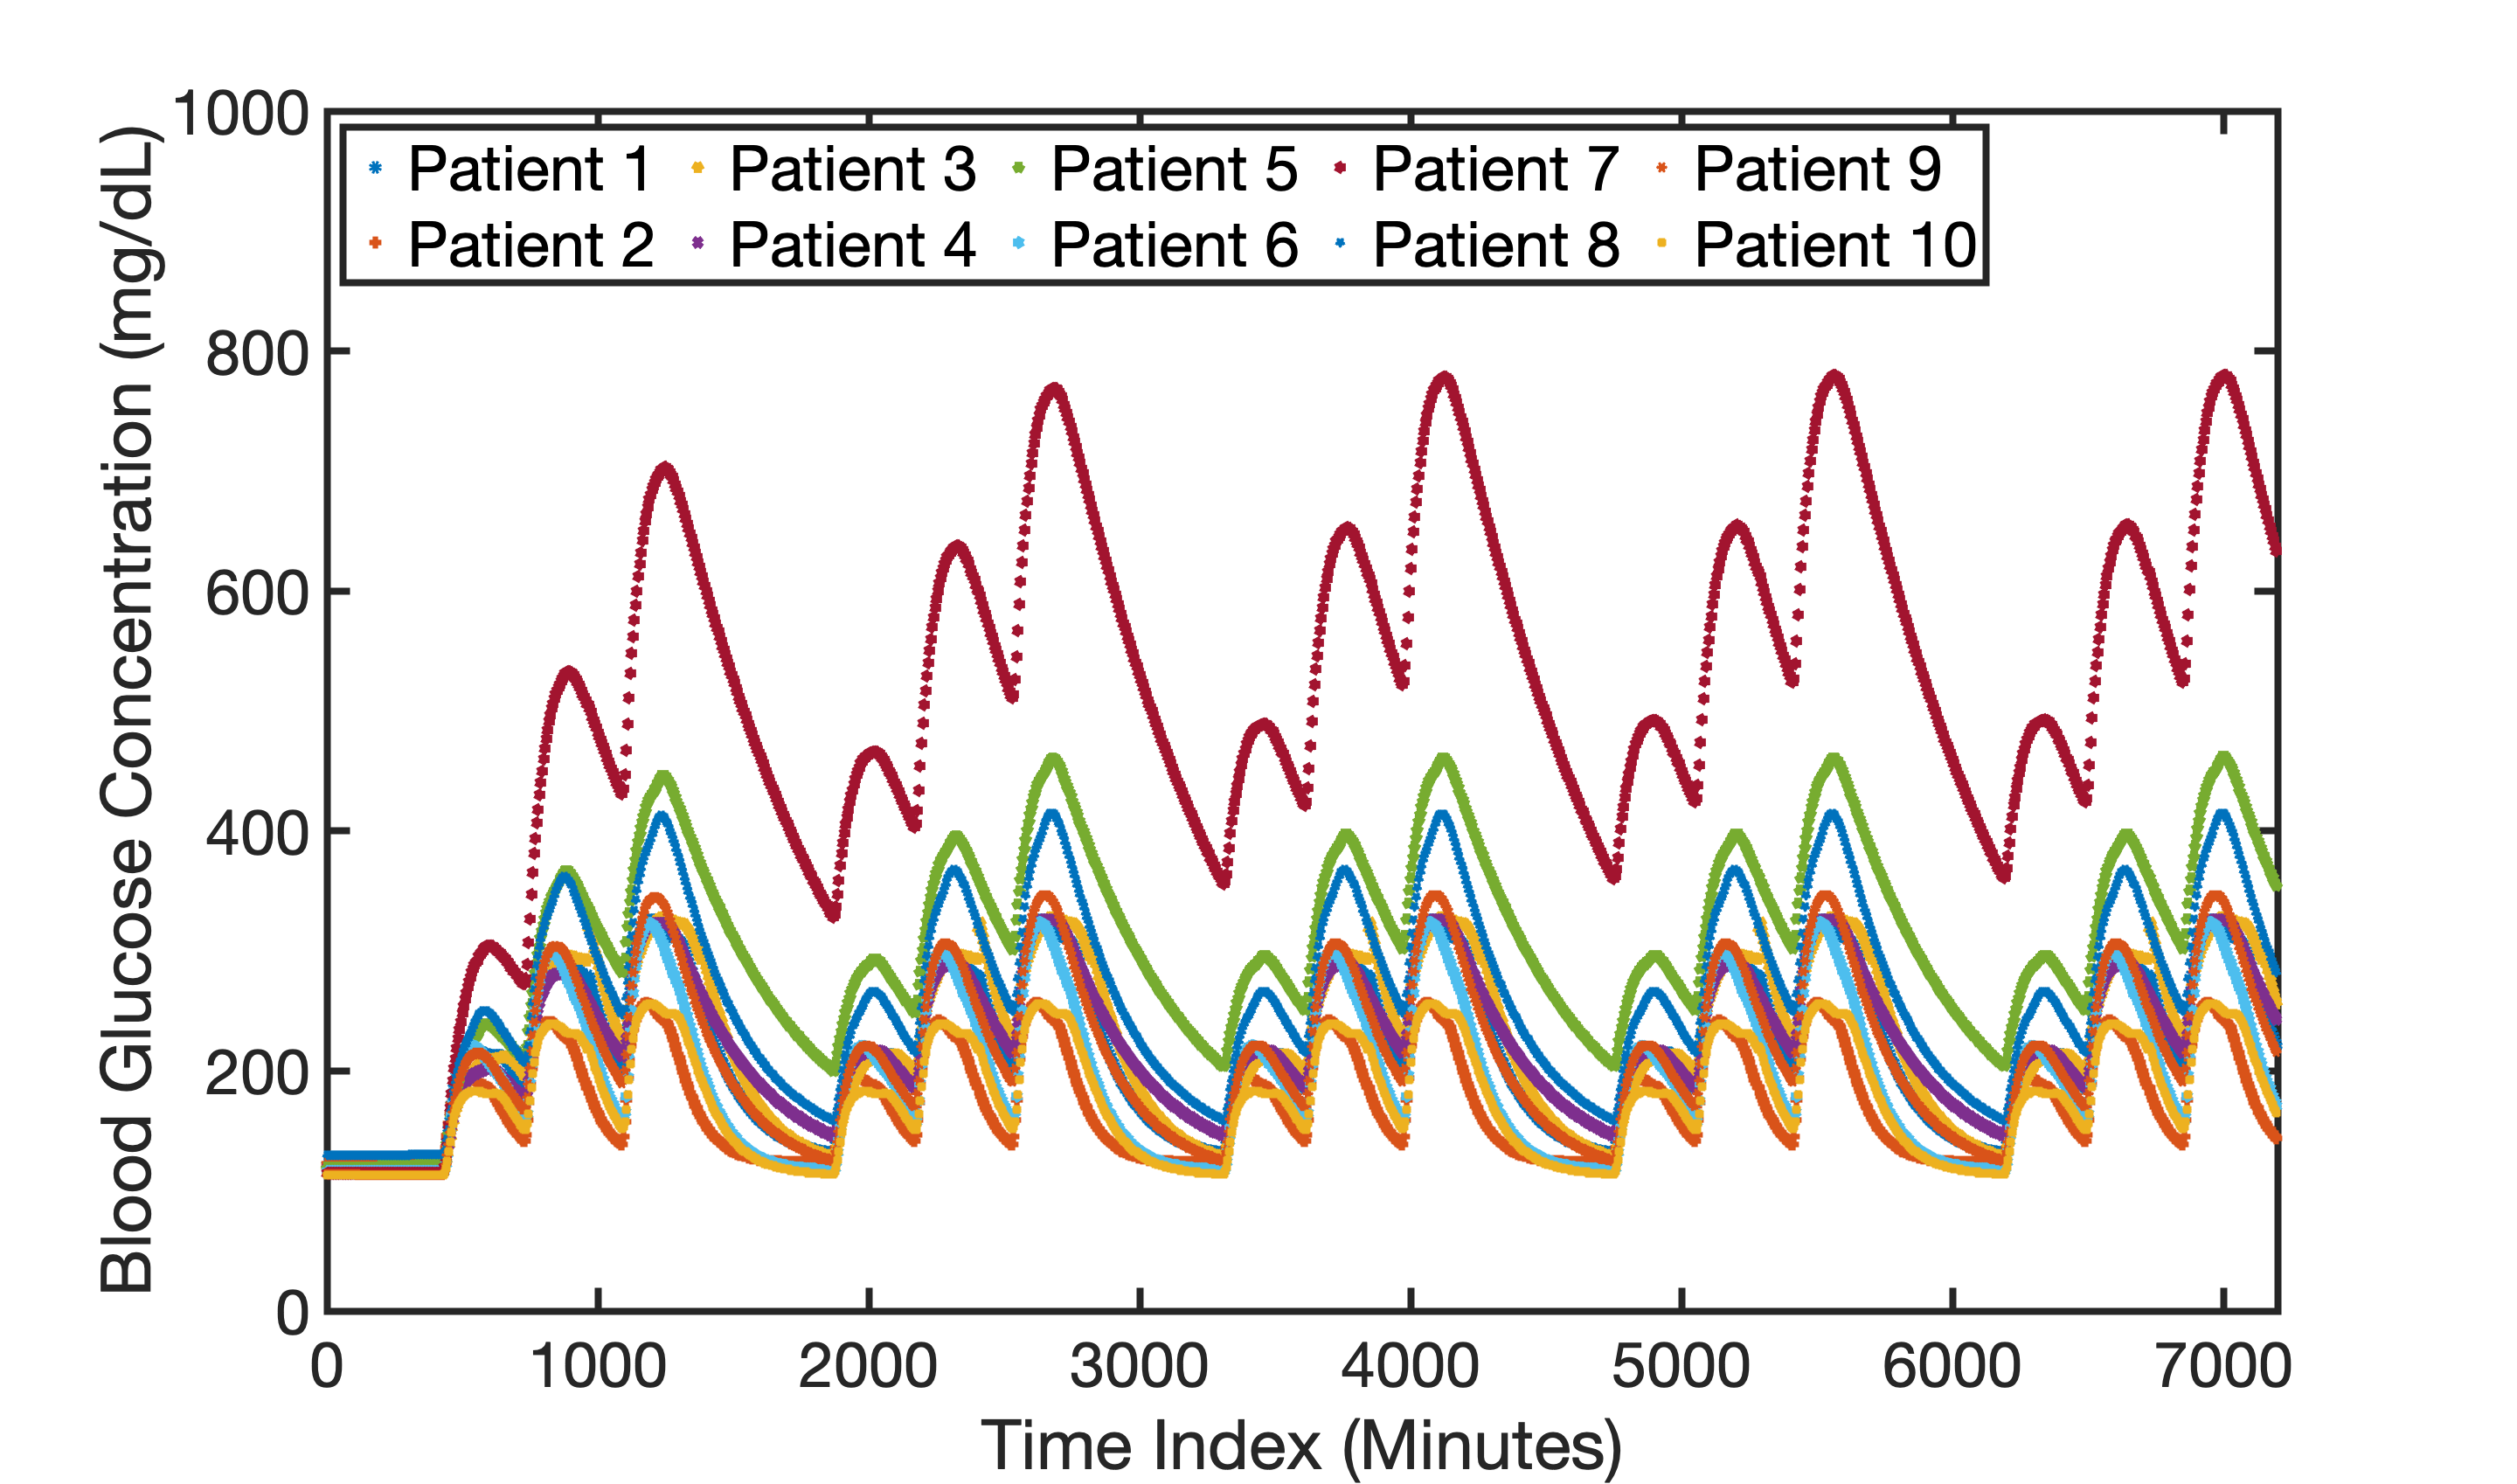
\includegraphics[width=\linewidth]{Figures/results/fda_data.png}
\caption{Blood glucose data of 10 patinets generated from UVA/Padova T1D simulator}
\label{fig:bergman}
\end{figure}



    \item Category 1: model plausibility plot for each fold + 4 validation data-model plots


\begin{figure}[H]
\centering

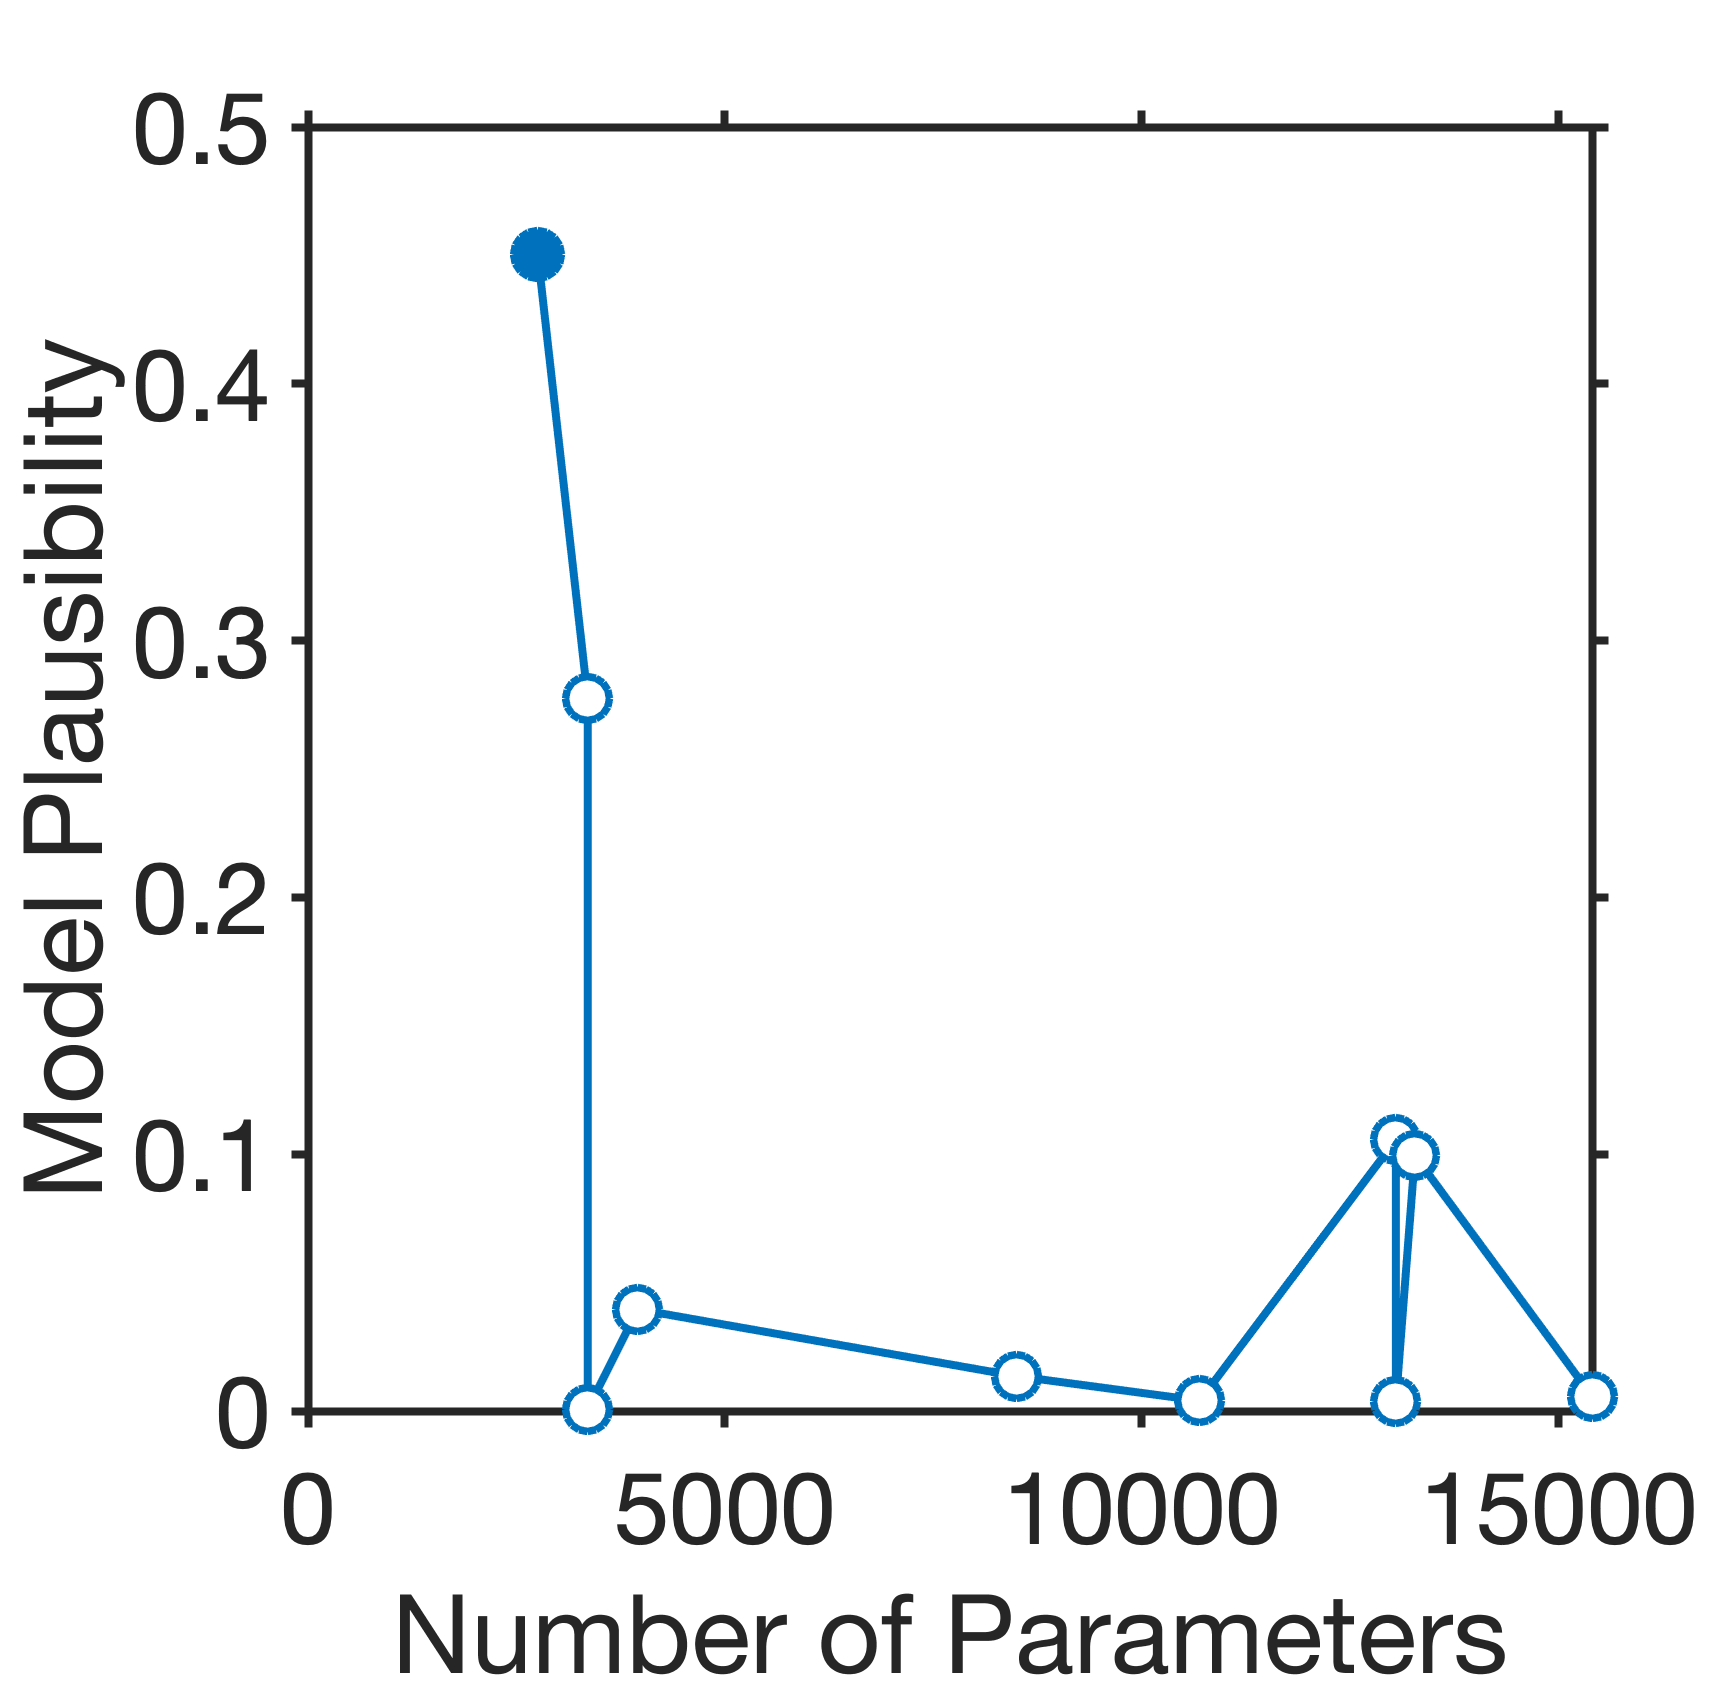
\includegraphics[width=0.19\textwidth]{Figures/Part B/cat1/fold1.png}\hfill
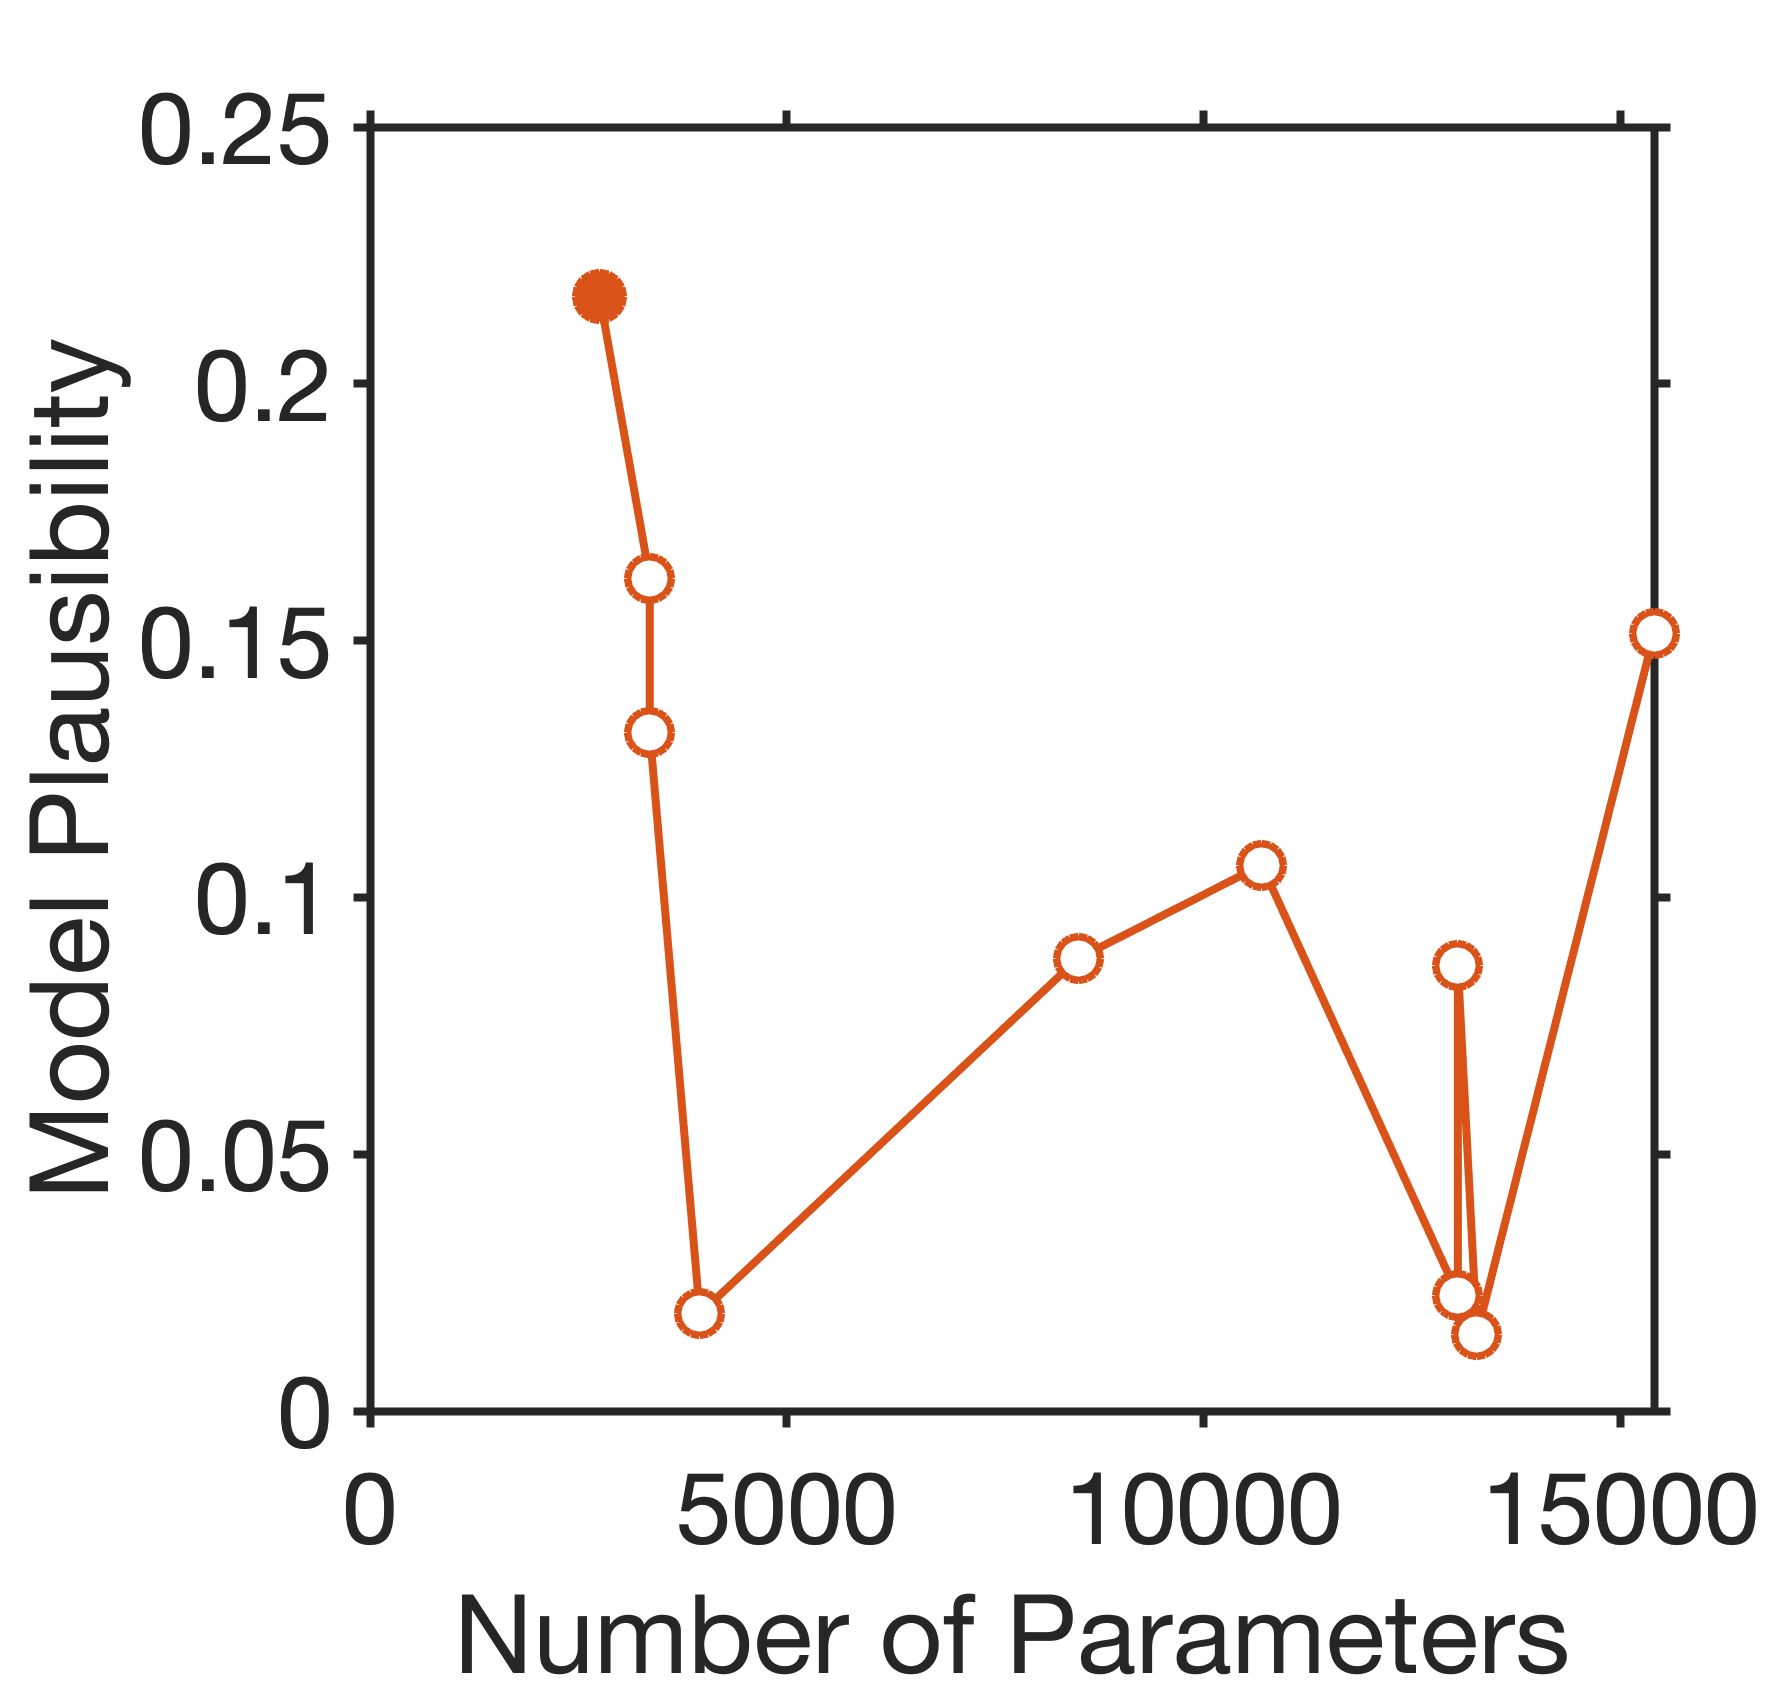
\includegraphics[width=0.19\textwidth]{Figures/Part B/cat1/fold2.png}\hfill
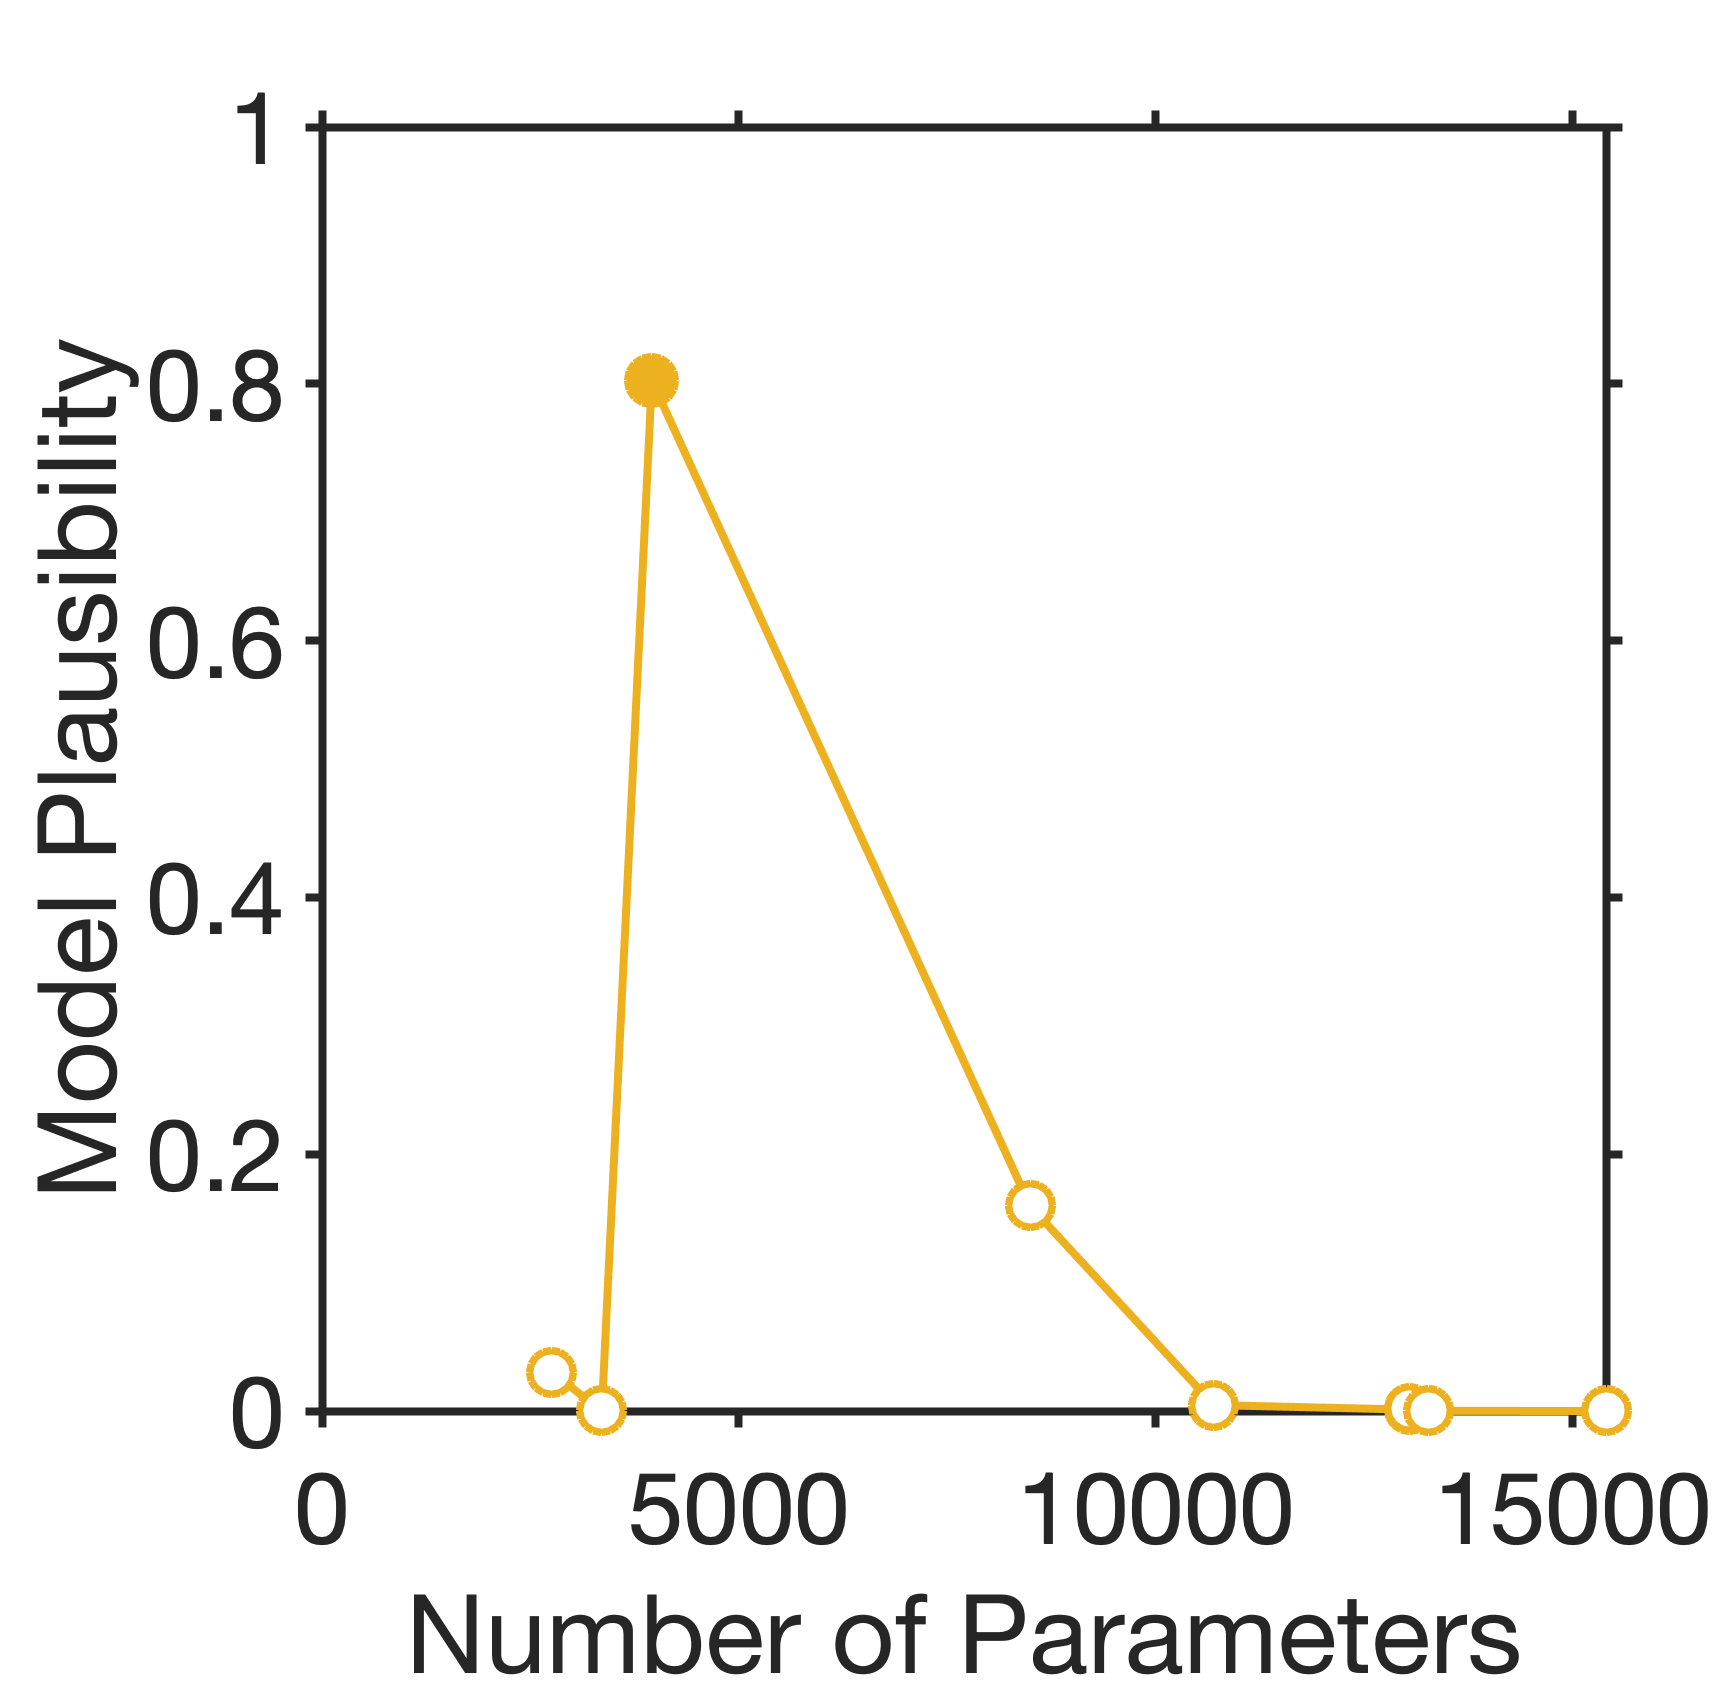
\includegraphics[width=0.19\textwidth]{Figures/Part B/cat1/fold3.png}\hfill
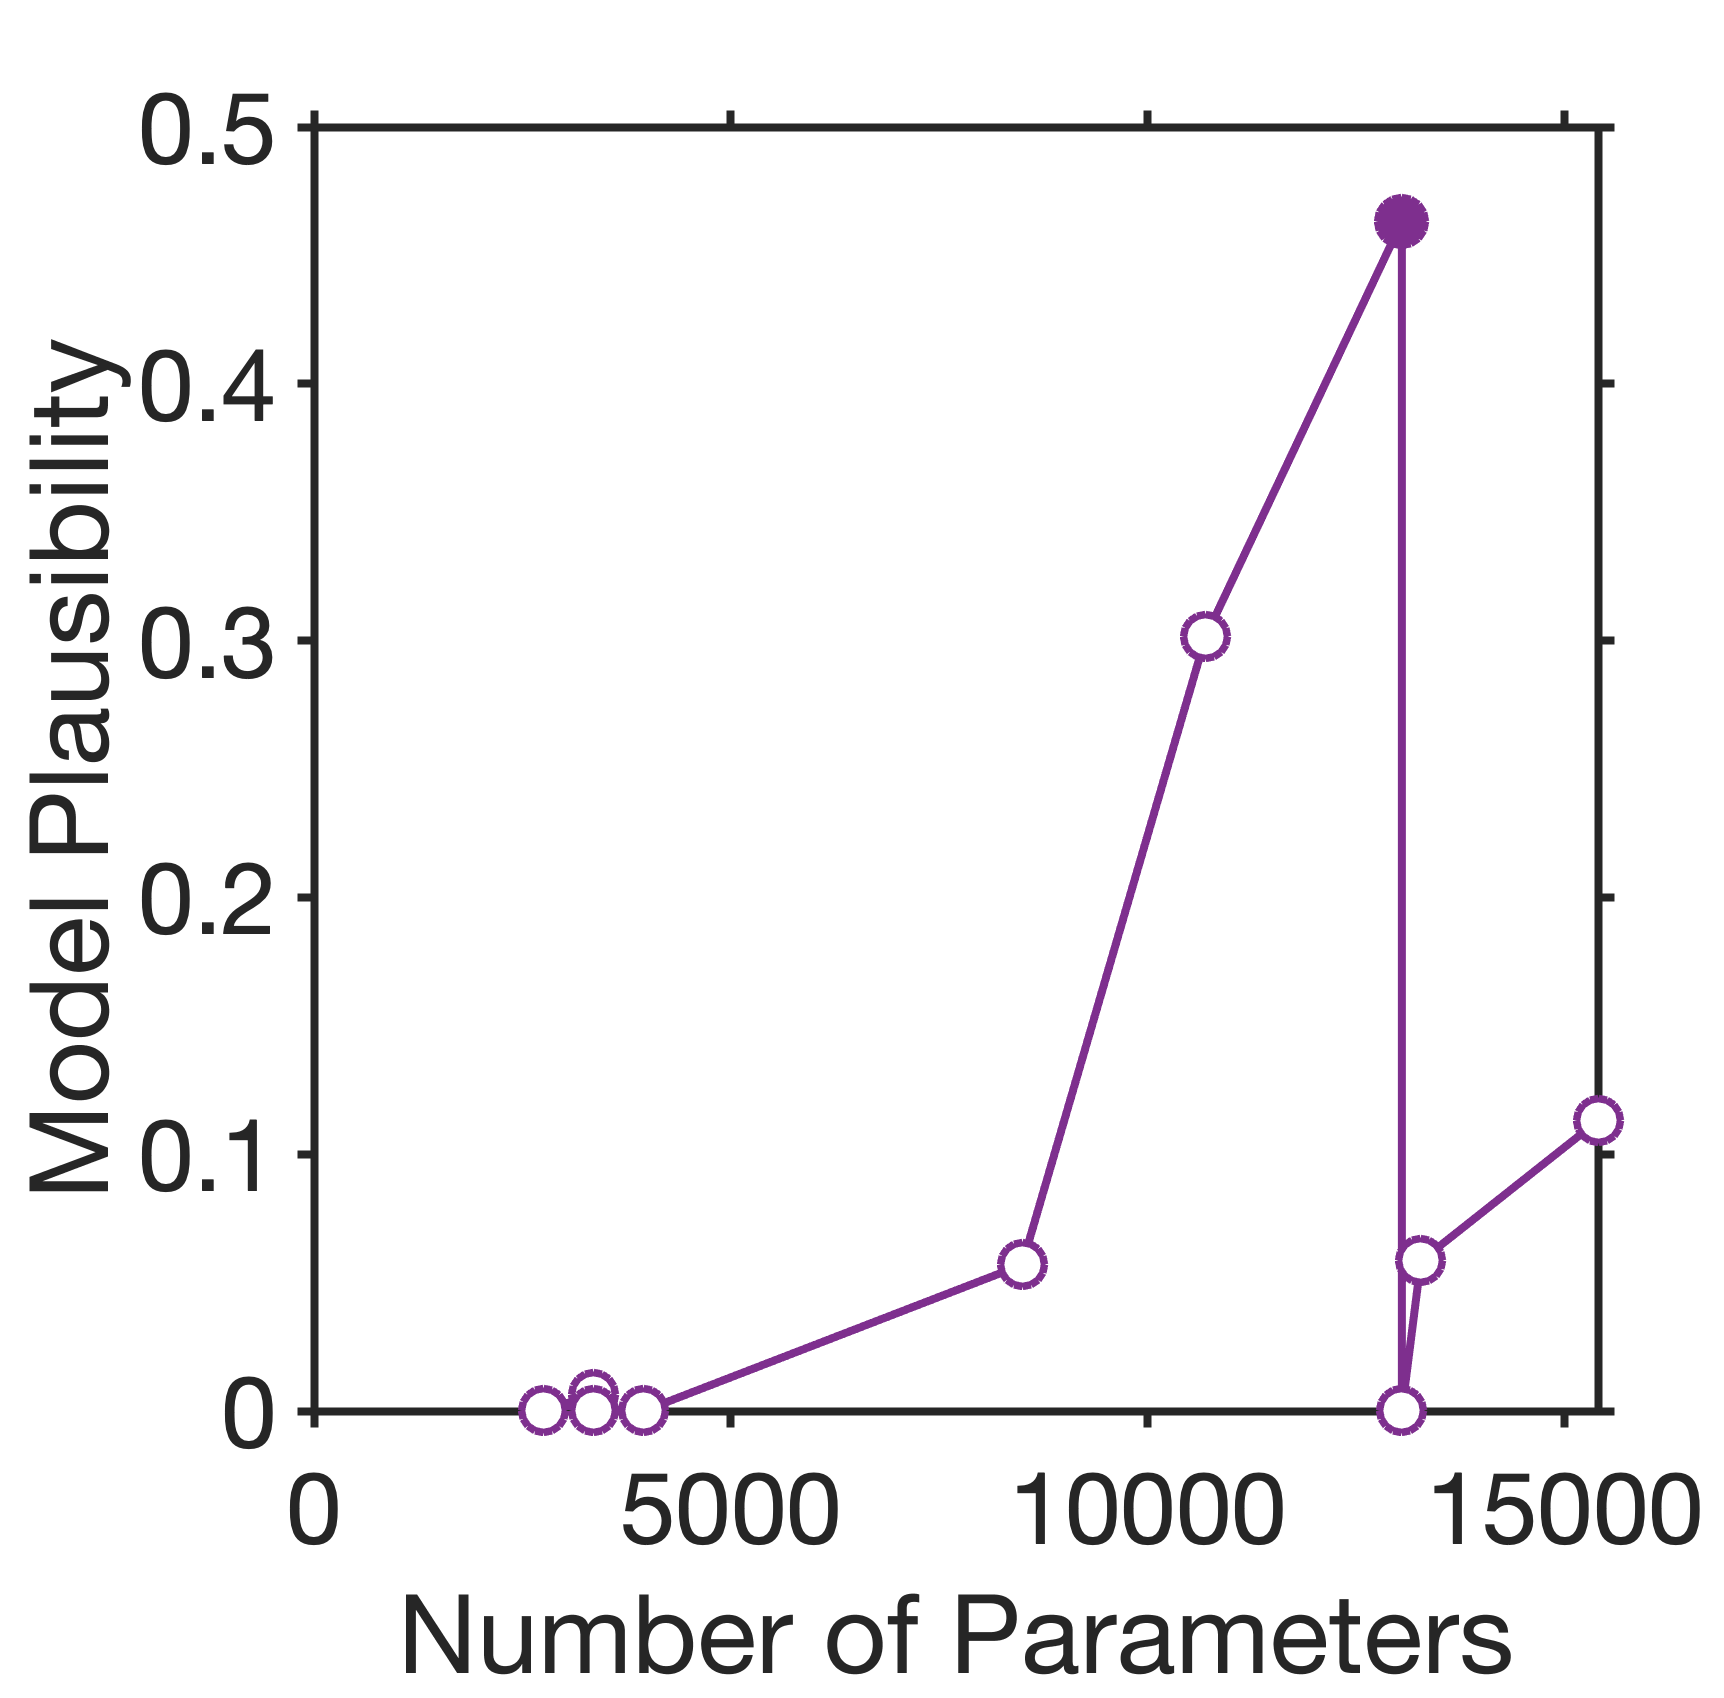
\includegraphics[width=0.19\textwidth]{Figures/Part B/cat1/fold4.png}\hfill
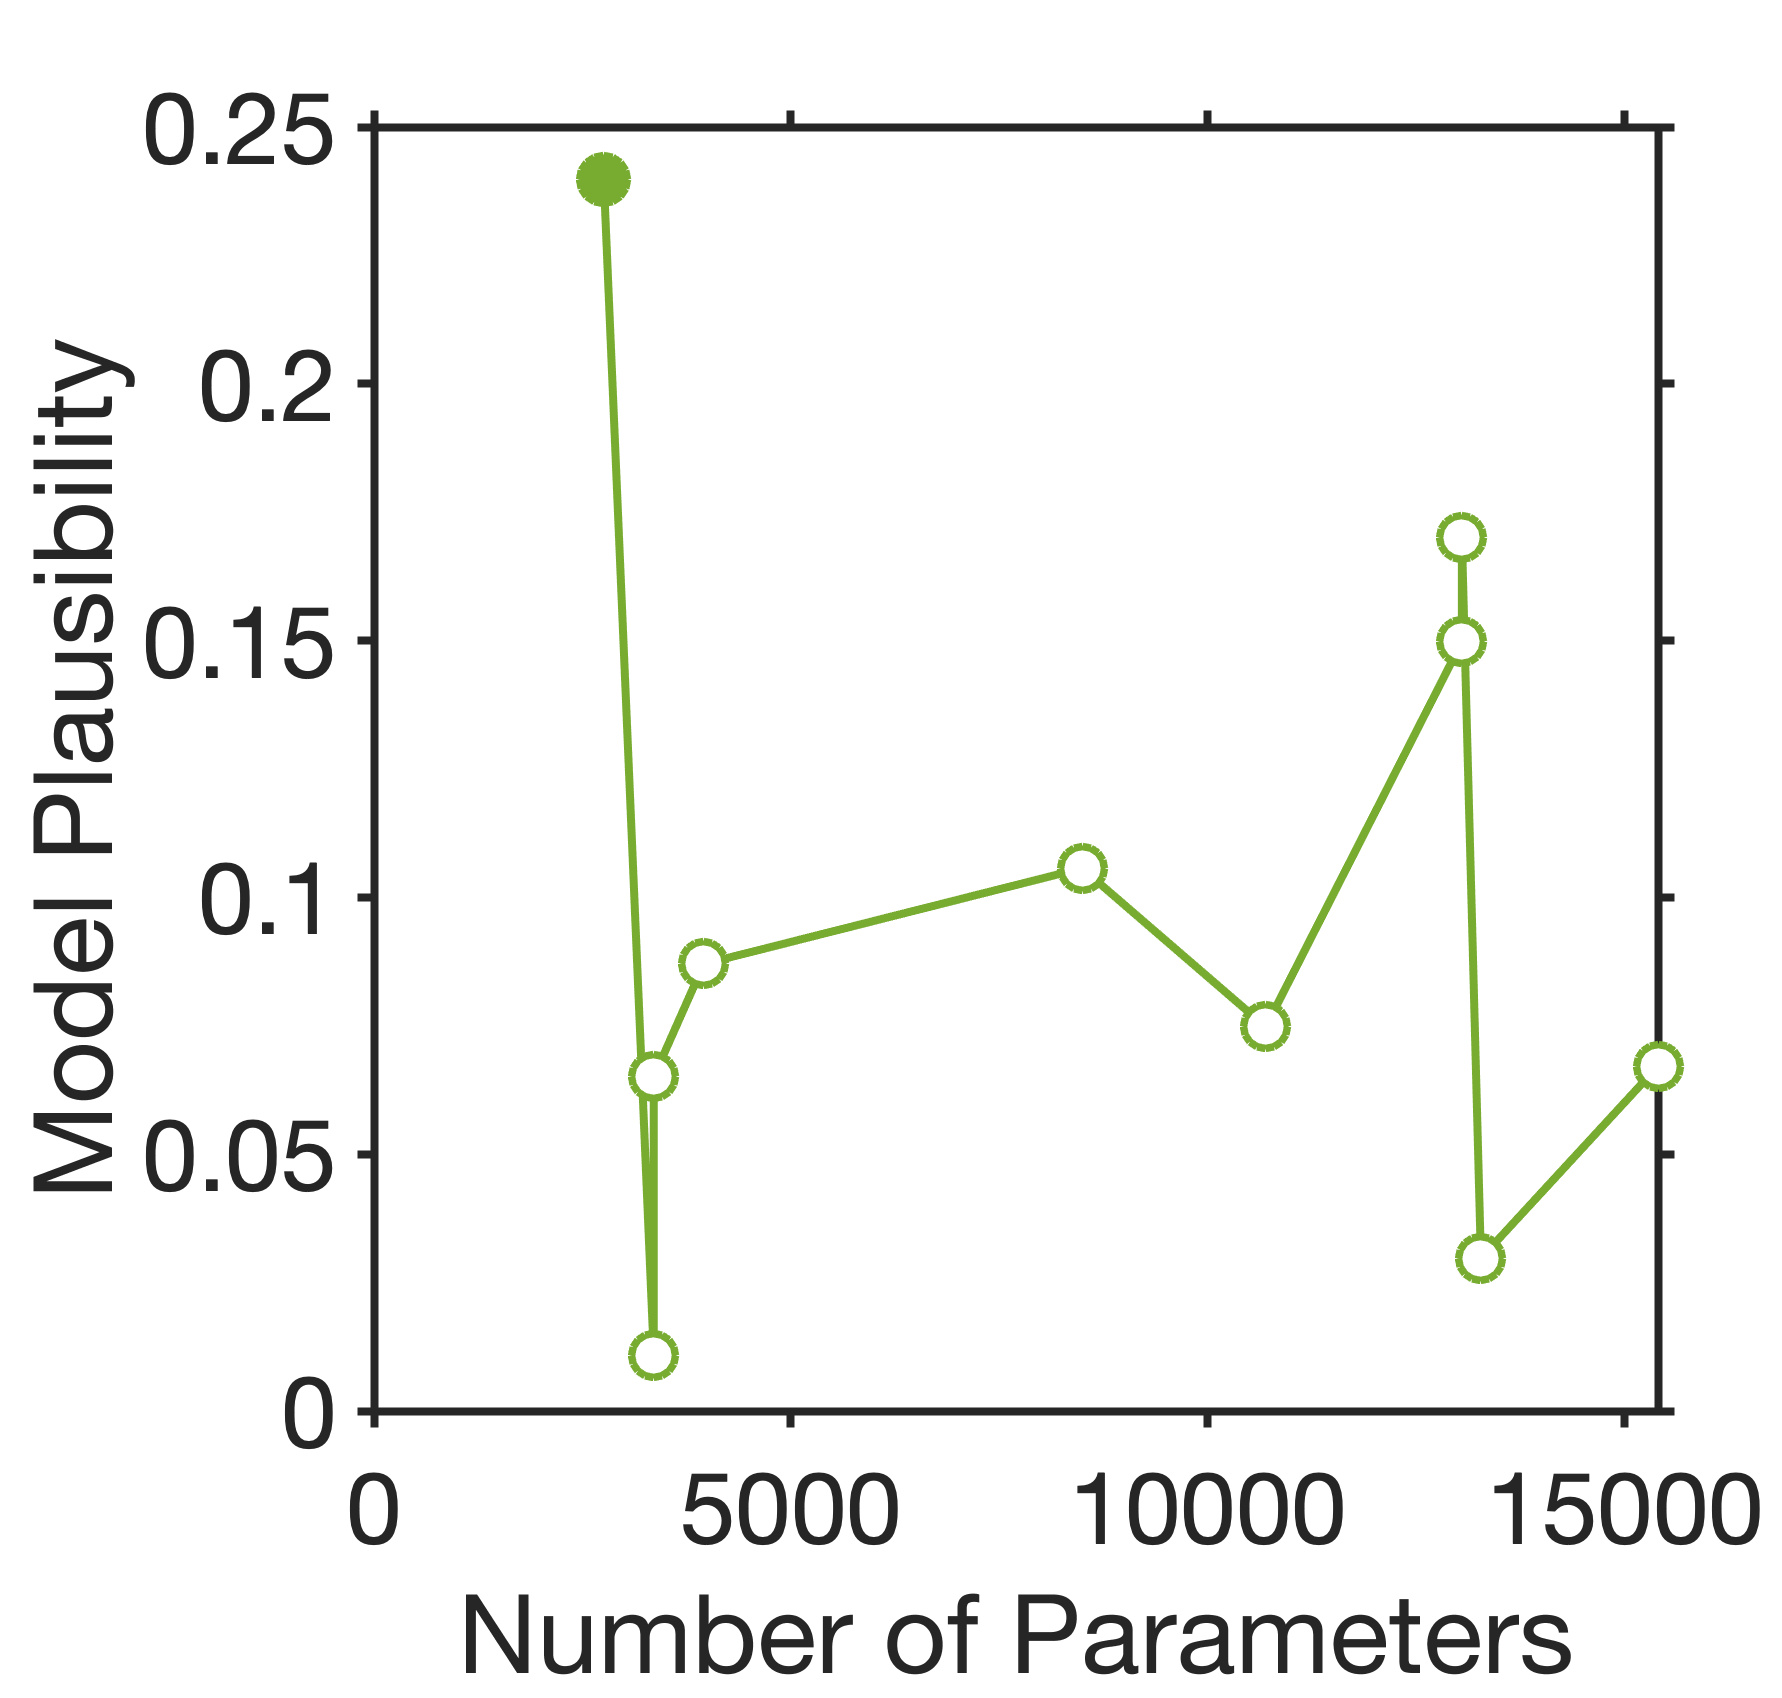
\includegraphics[width=0.19\textwidth]{Figures/Part B/cat1/fold5.png}

\caption{Model Plausibility plotted against number of parameters for all folds in category 1 (from Lett to right: fold 1 to fold 5 respectively)}
\label{fig:cat1_plausibility}
\end{figure}


Category~1 contains the smallest B-TCN candidates (lowest parameters) that still satisfy the receptive-field feasibility constraints. \autoref{fig:cat1_plausibility} summarizes how model plausibility varies with the number of parameters across folds. Within this category, plausibility tends to concentrate on a small subset of architectures, indicating that the evidence favors specific design choices. However, the key observation is that models in Category~1 are still capacity-limited in an absolute sense: their parameters are insufficient to reliably represent the blood glucose dynamics. This limitation is reflected in the prediction windows of \autoref{fig:cat1-pred}. Across representative architectures, the forecasts windows frequently violate the acceptance tolerance which are flagged in red.




\begin{figure}[H]
\centering

\begin{minipage}[t]{0.48\textwidth}
  \centering
  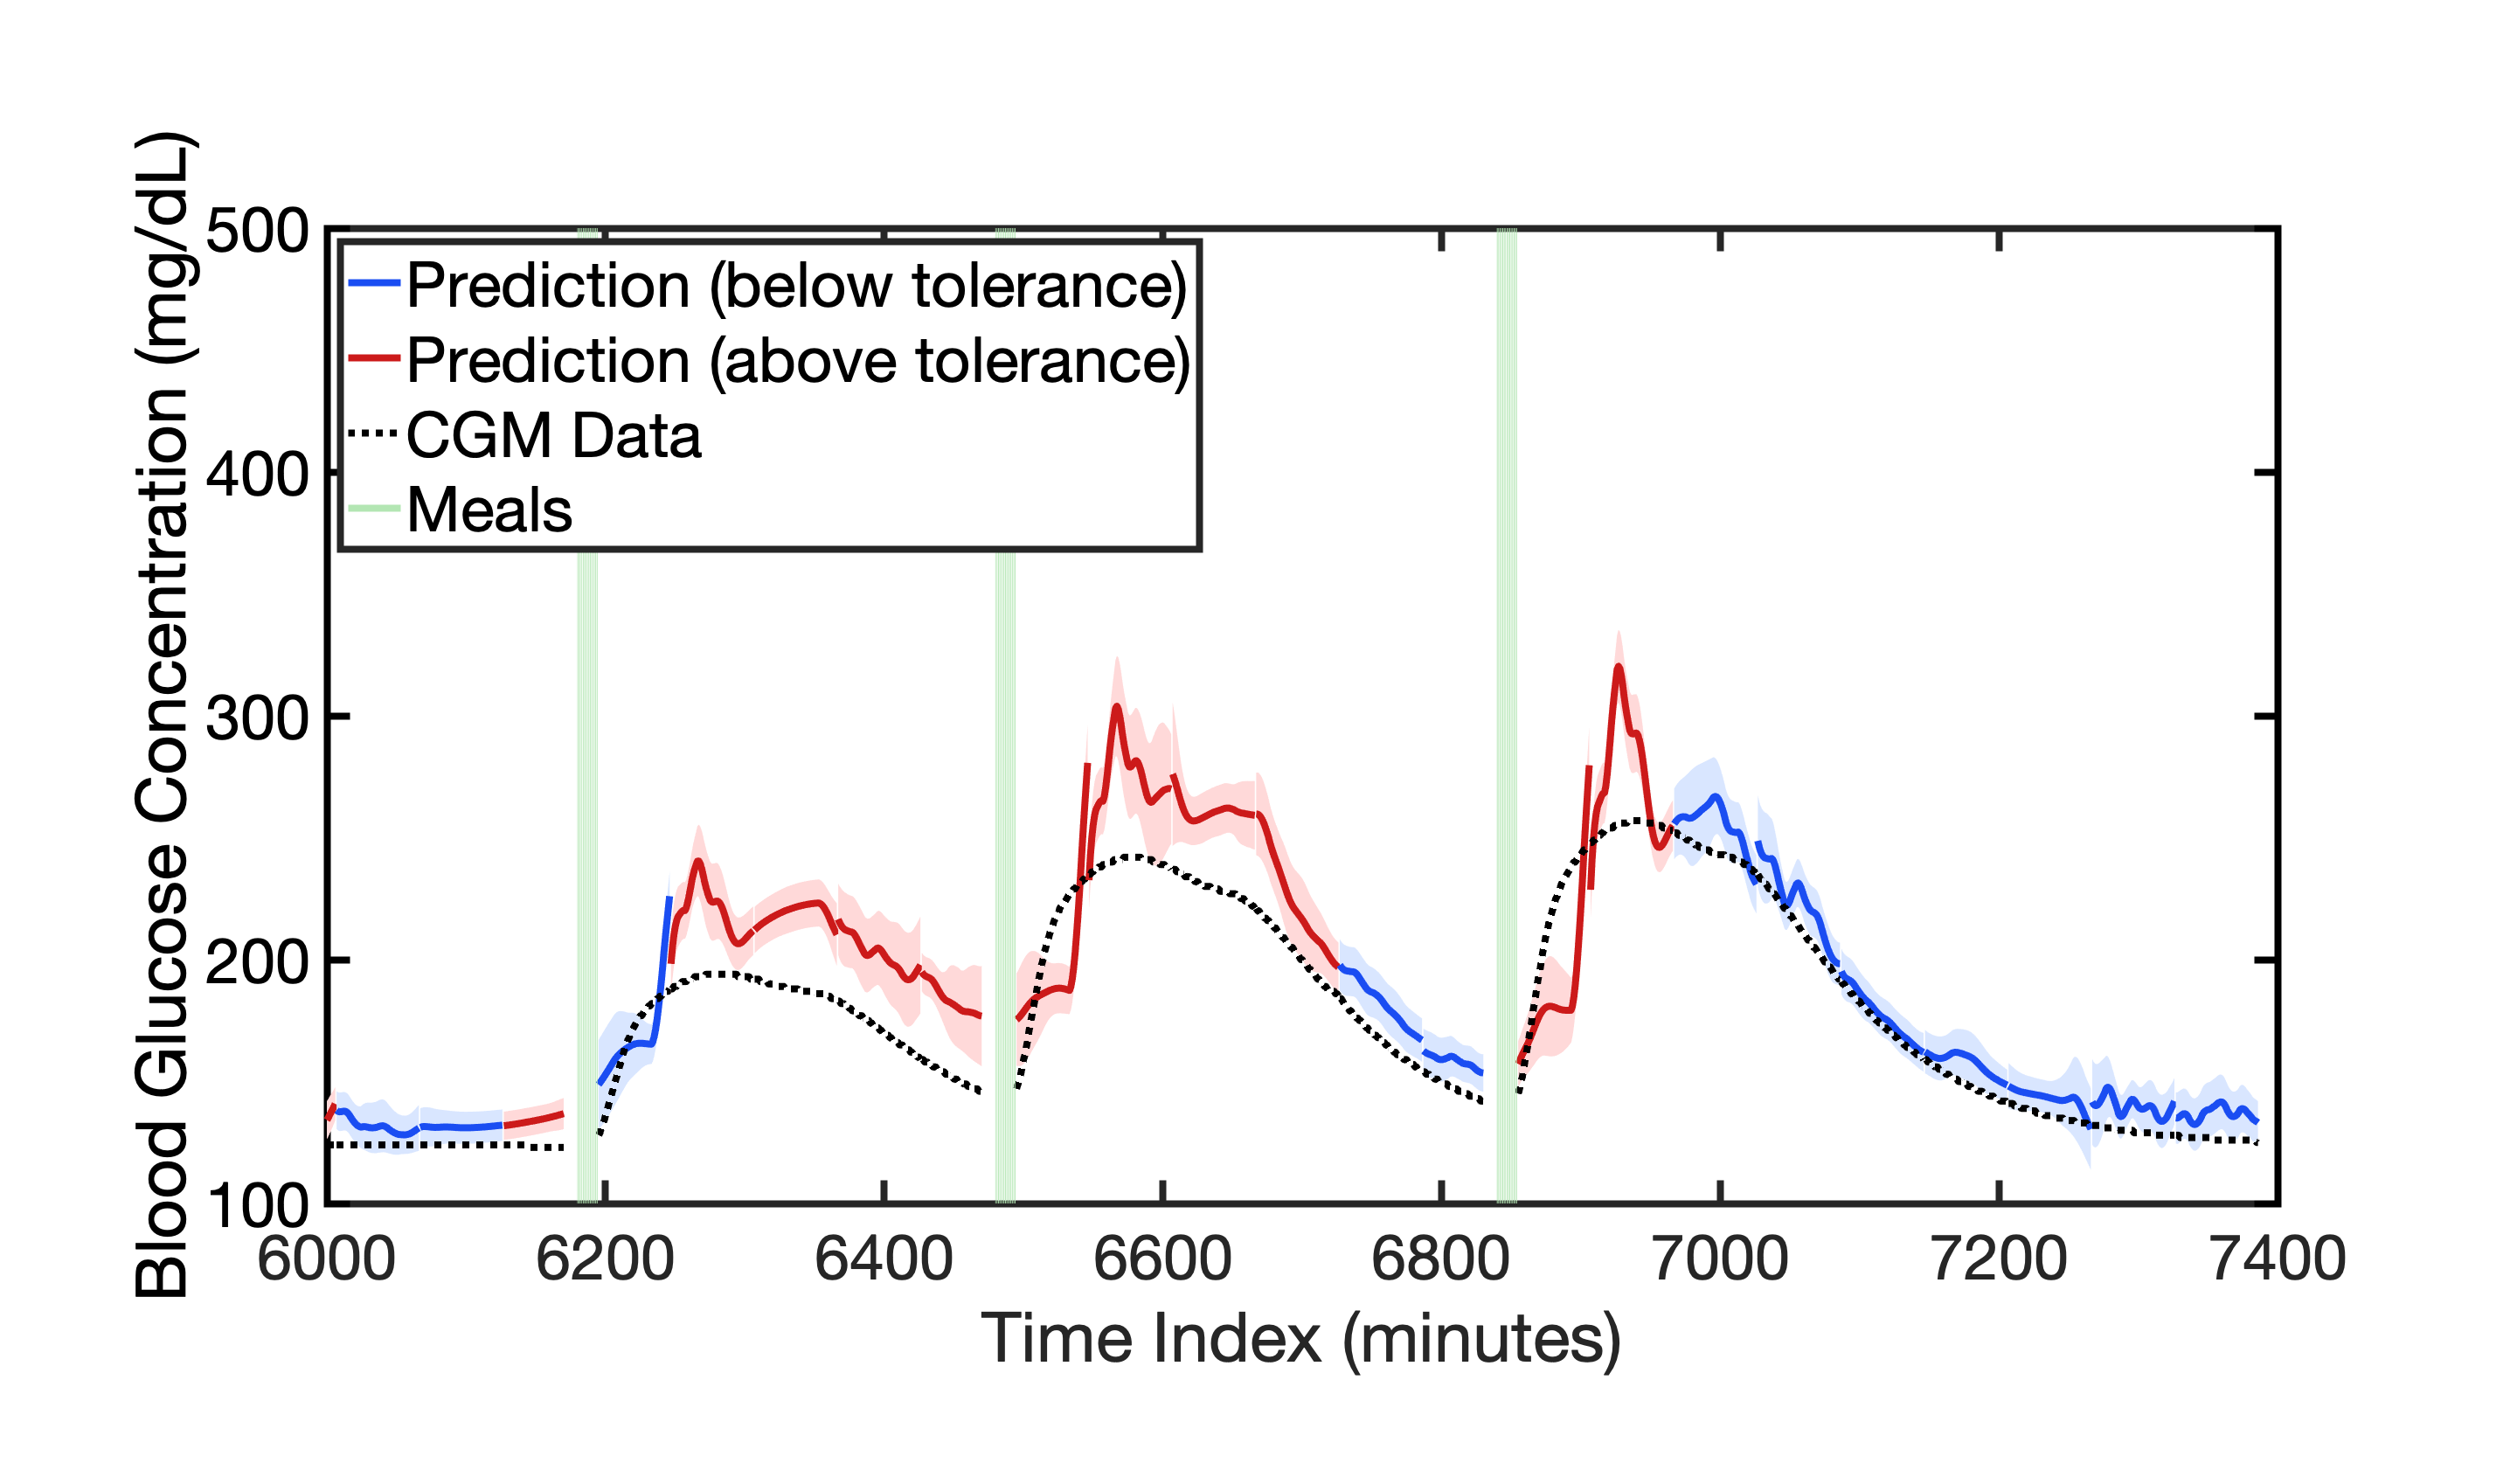
\includegraphics[width=\linewidth]{Figures/Part B/cat1/p2_c1.png}
  \caption*{(a)}
\end{minipage}\hfill
\begin{minipage}[t]{0.48\textwidth}
  \centering
  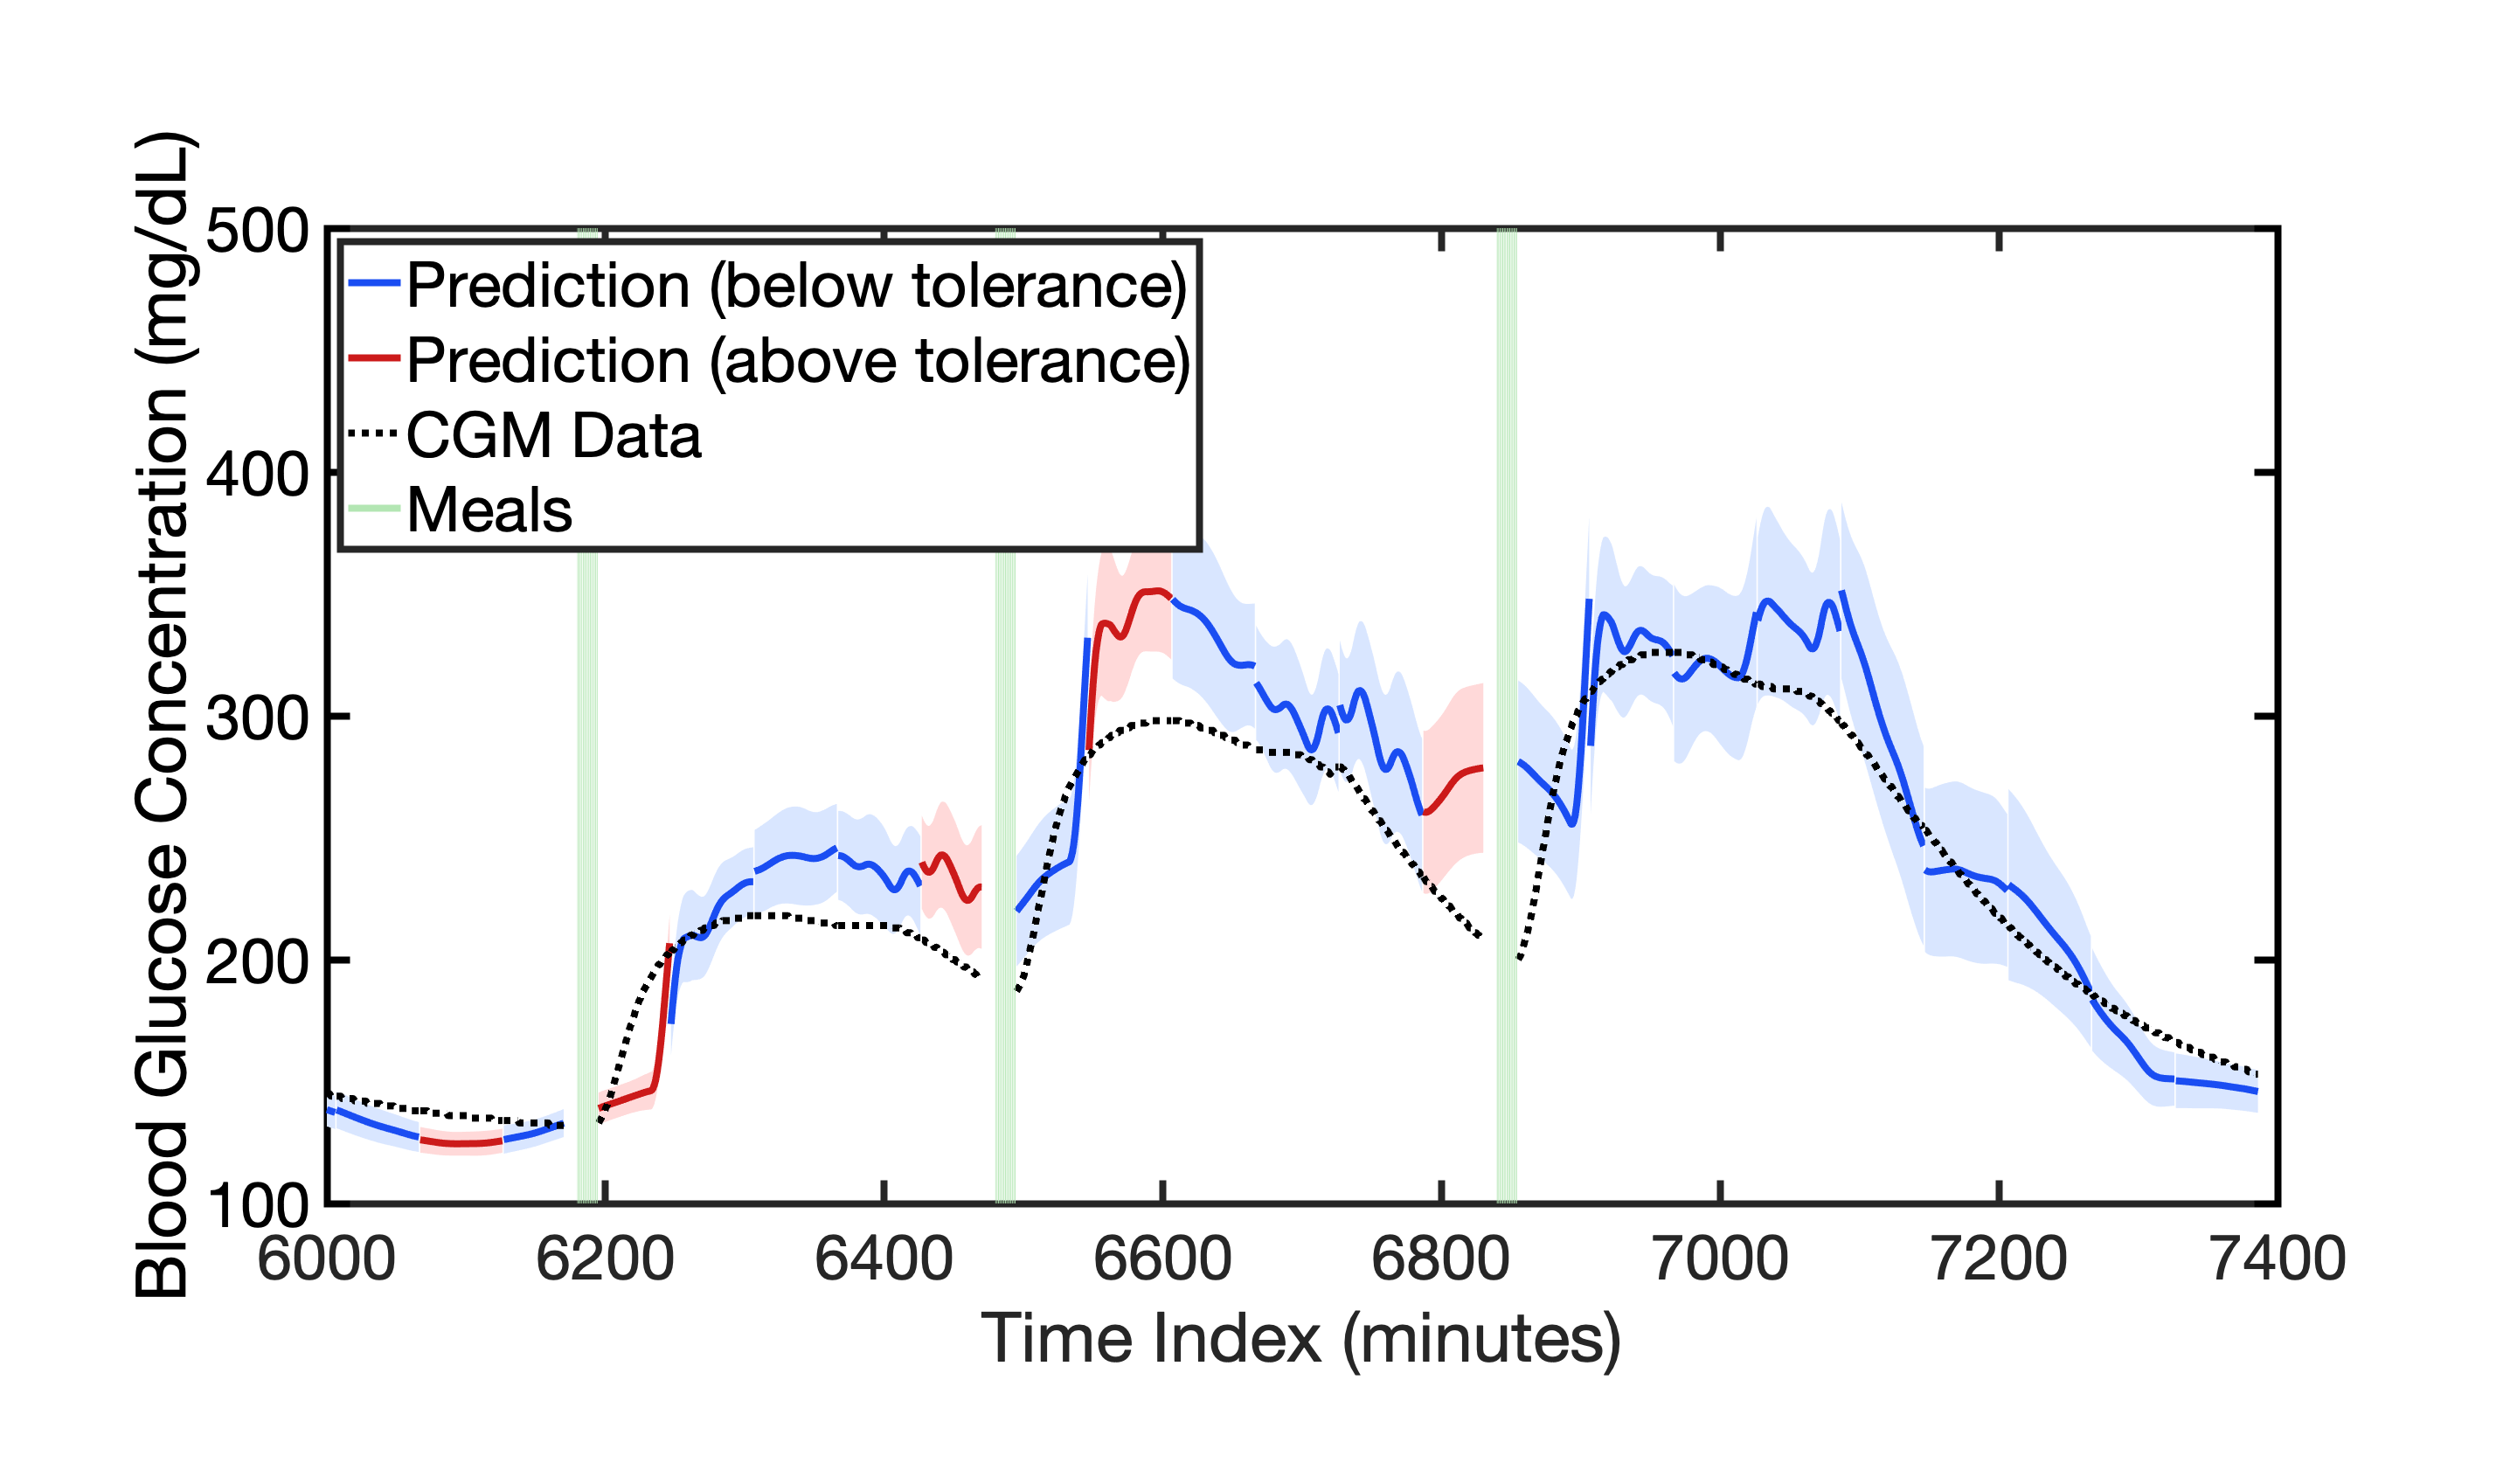
\includegraphics[width=\linewidth]{Figures/Part B/cat1/p1_c1.png}
  \caption*{(b)}
\end{minipage}

\begin{minipage}[t]{0.48\textwidth}
  \centering
  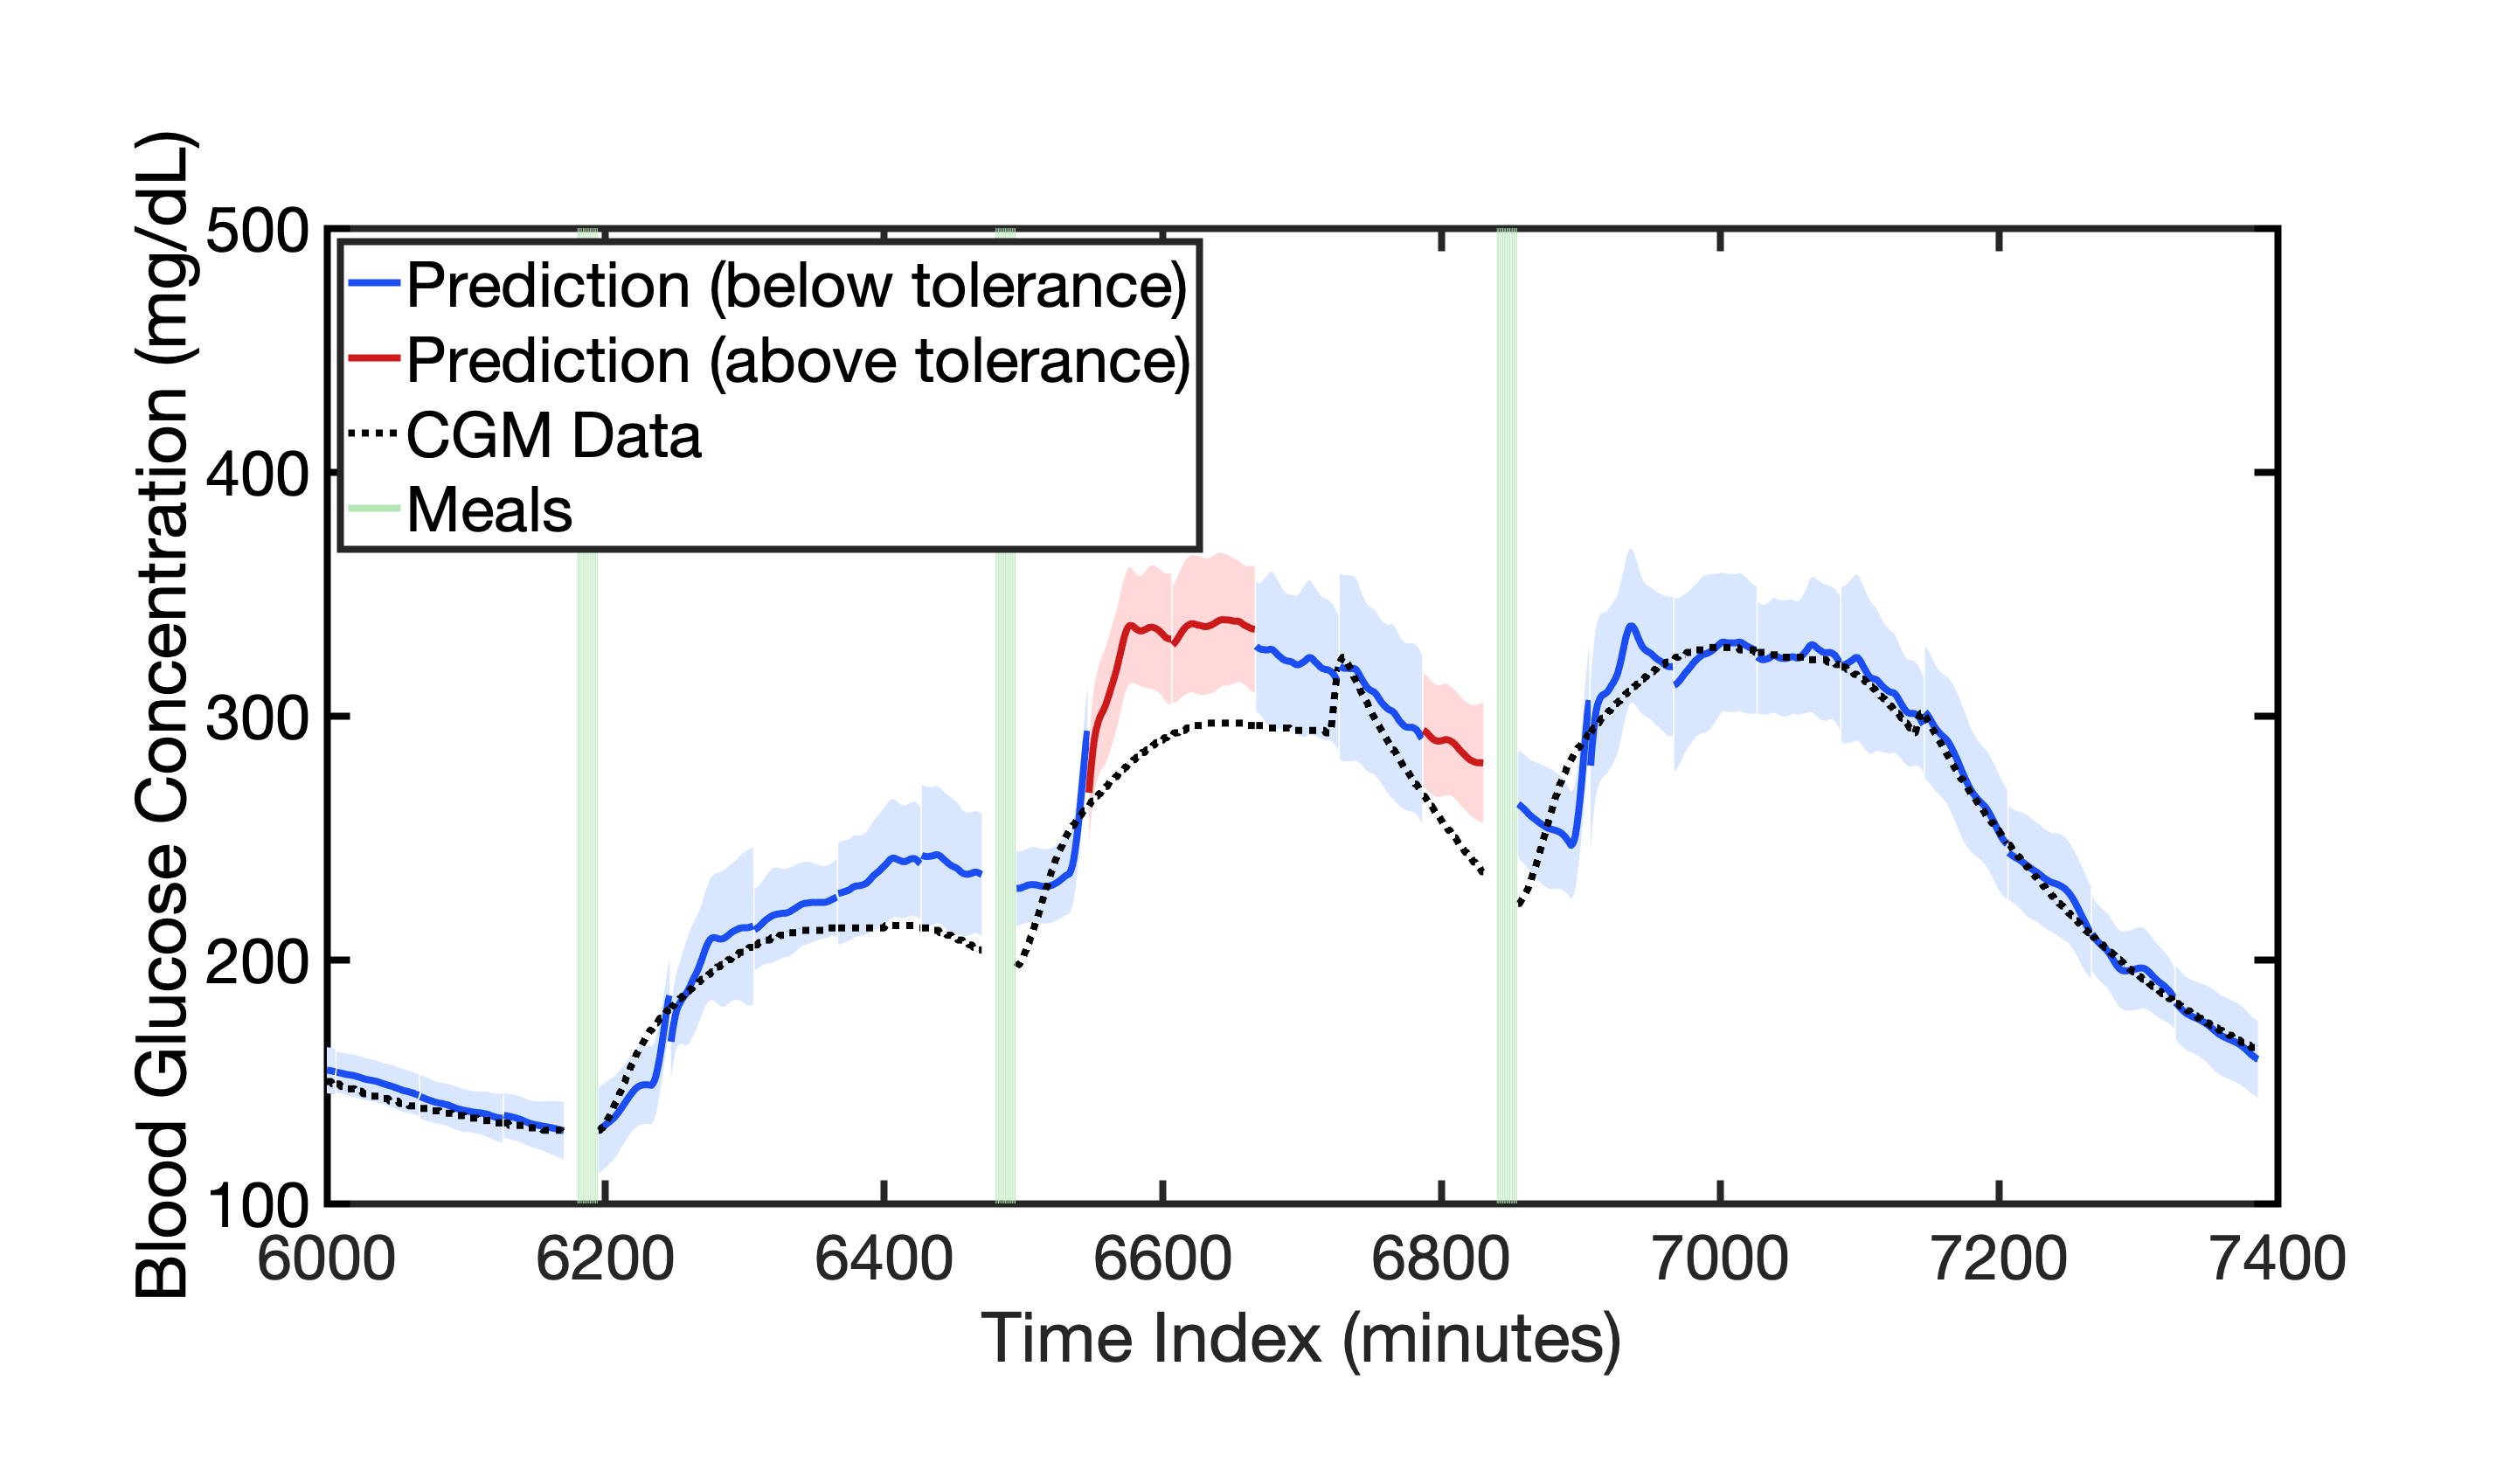
\includegraphics[width=\linewidth]{Figures/Part B/cat1/p3_c1.png}
  \caption*{(c)}
\end{minipage}\hfill
\begin{minipage}[t]{0.48\textwidth}
  \centering
  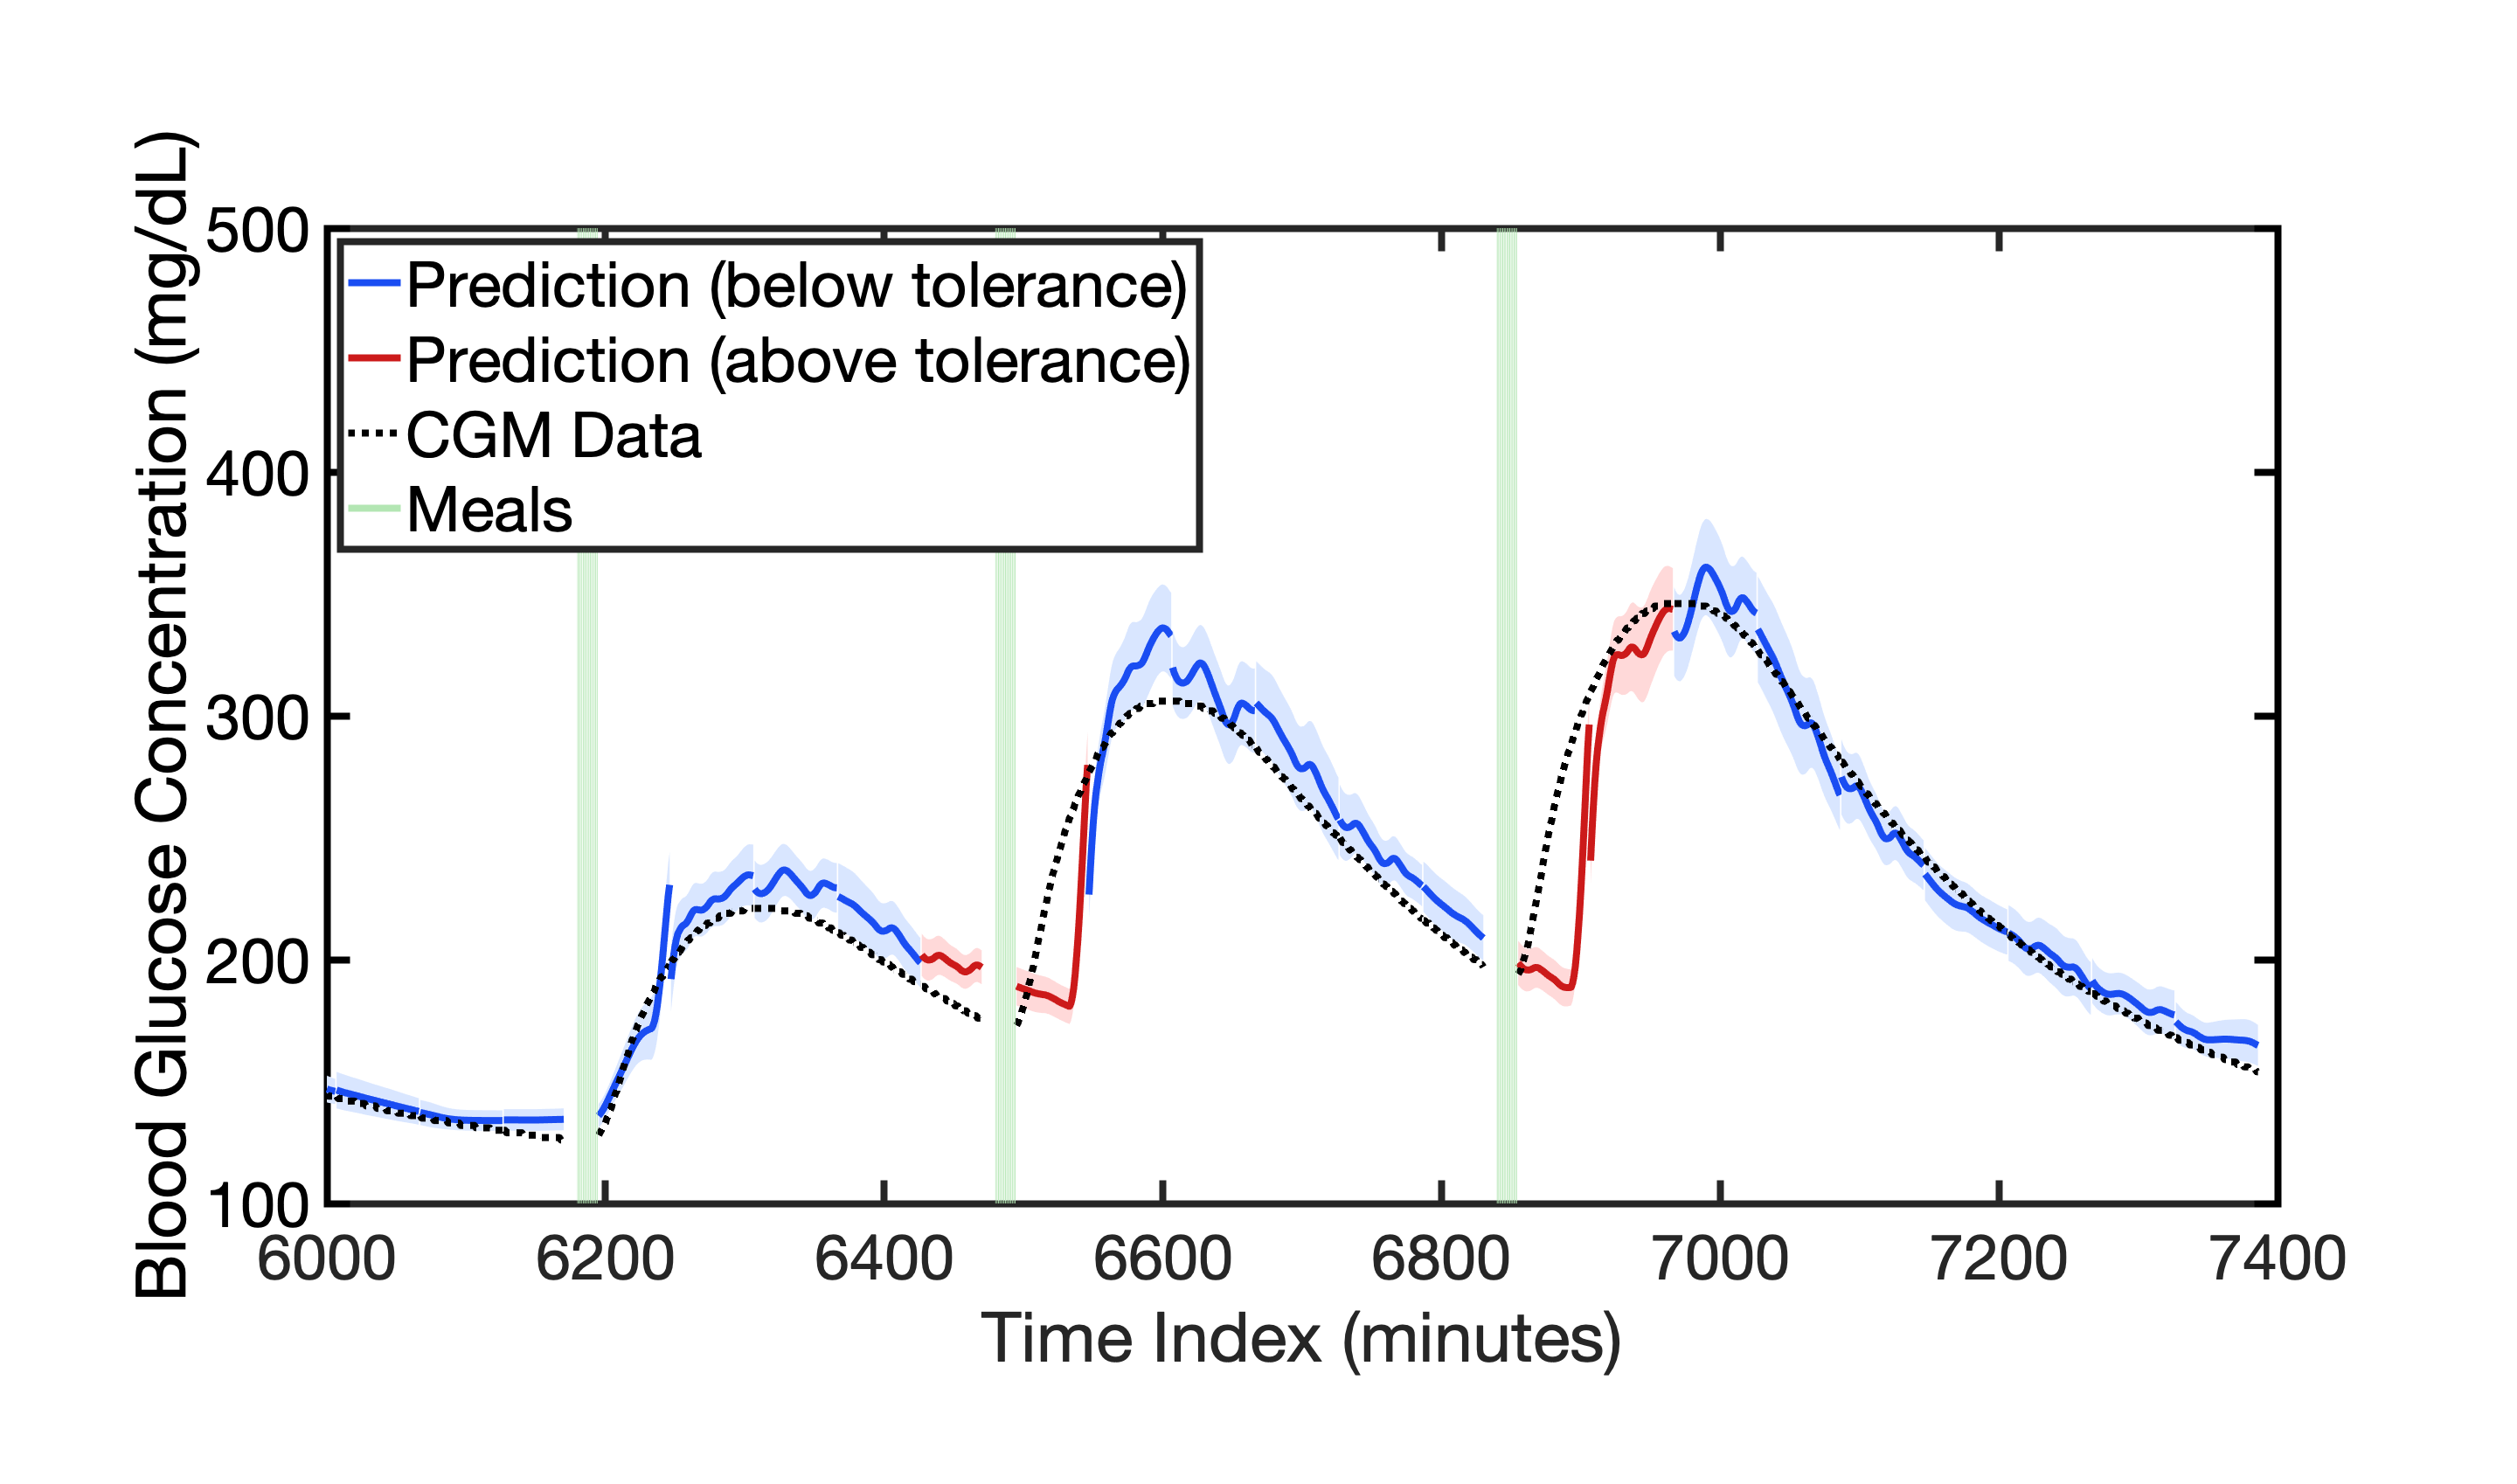
\includegraphics[width=\linewidth]{Figures/Part B/cat1/p9_c1.png}
  \caption*{(d)}
\end{minipage}

\caption{(a) Patient 2 from fold 3, Architecture: $Cat_1Arch_4$, (b) Patient 1 from fold 3, Architecture: $Cat_1Arch_4$, (c) Patient 3 from fold 4, Architecture: $Cat_1Arch_6$, and Patient 9 from fold 1, Architecture: $Cat_1Arch_1$.}
\label{fig:cat1-pred}
\end{figure}


    \item Category 2 (most important): sigma noise and model plausibility plot for each fold + two 2x2 validation data-model plots


\begin{figure}[H]
\centering

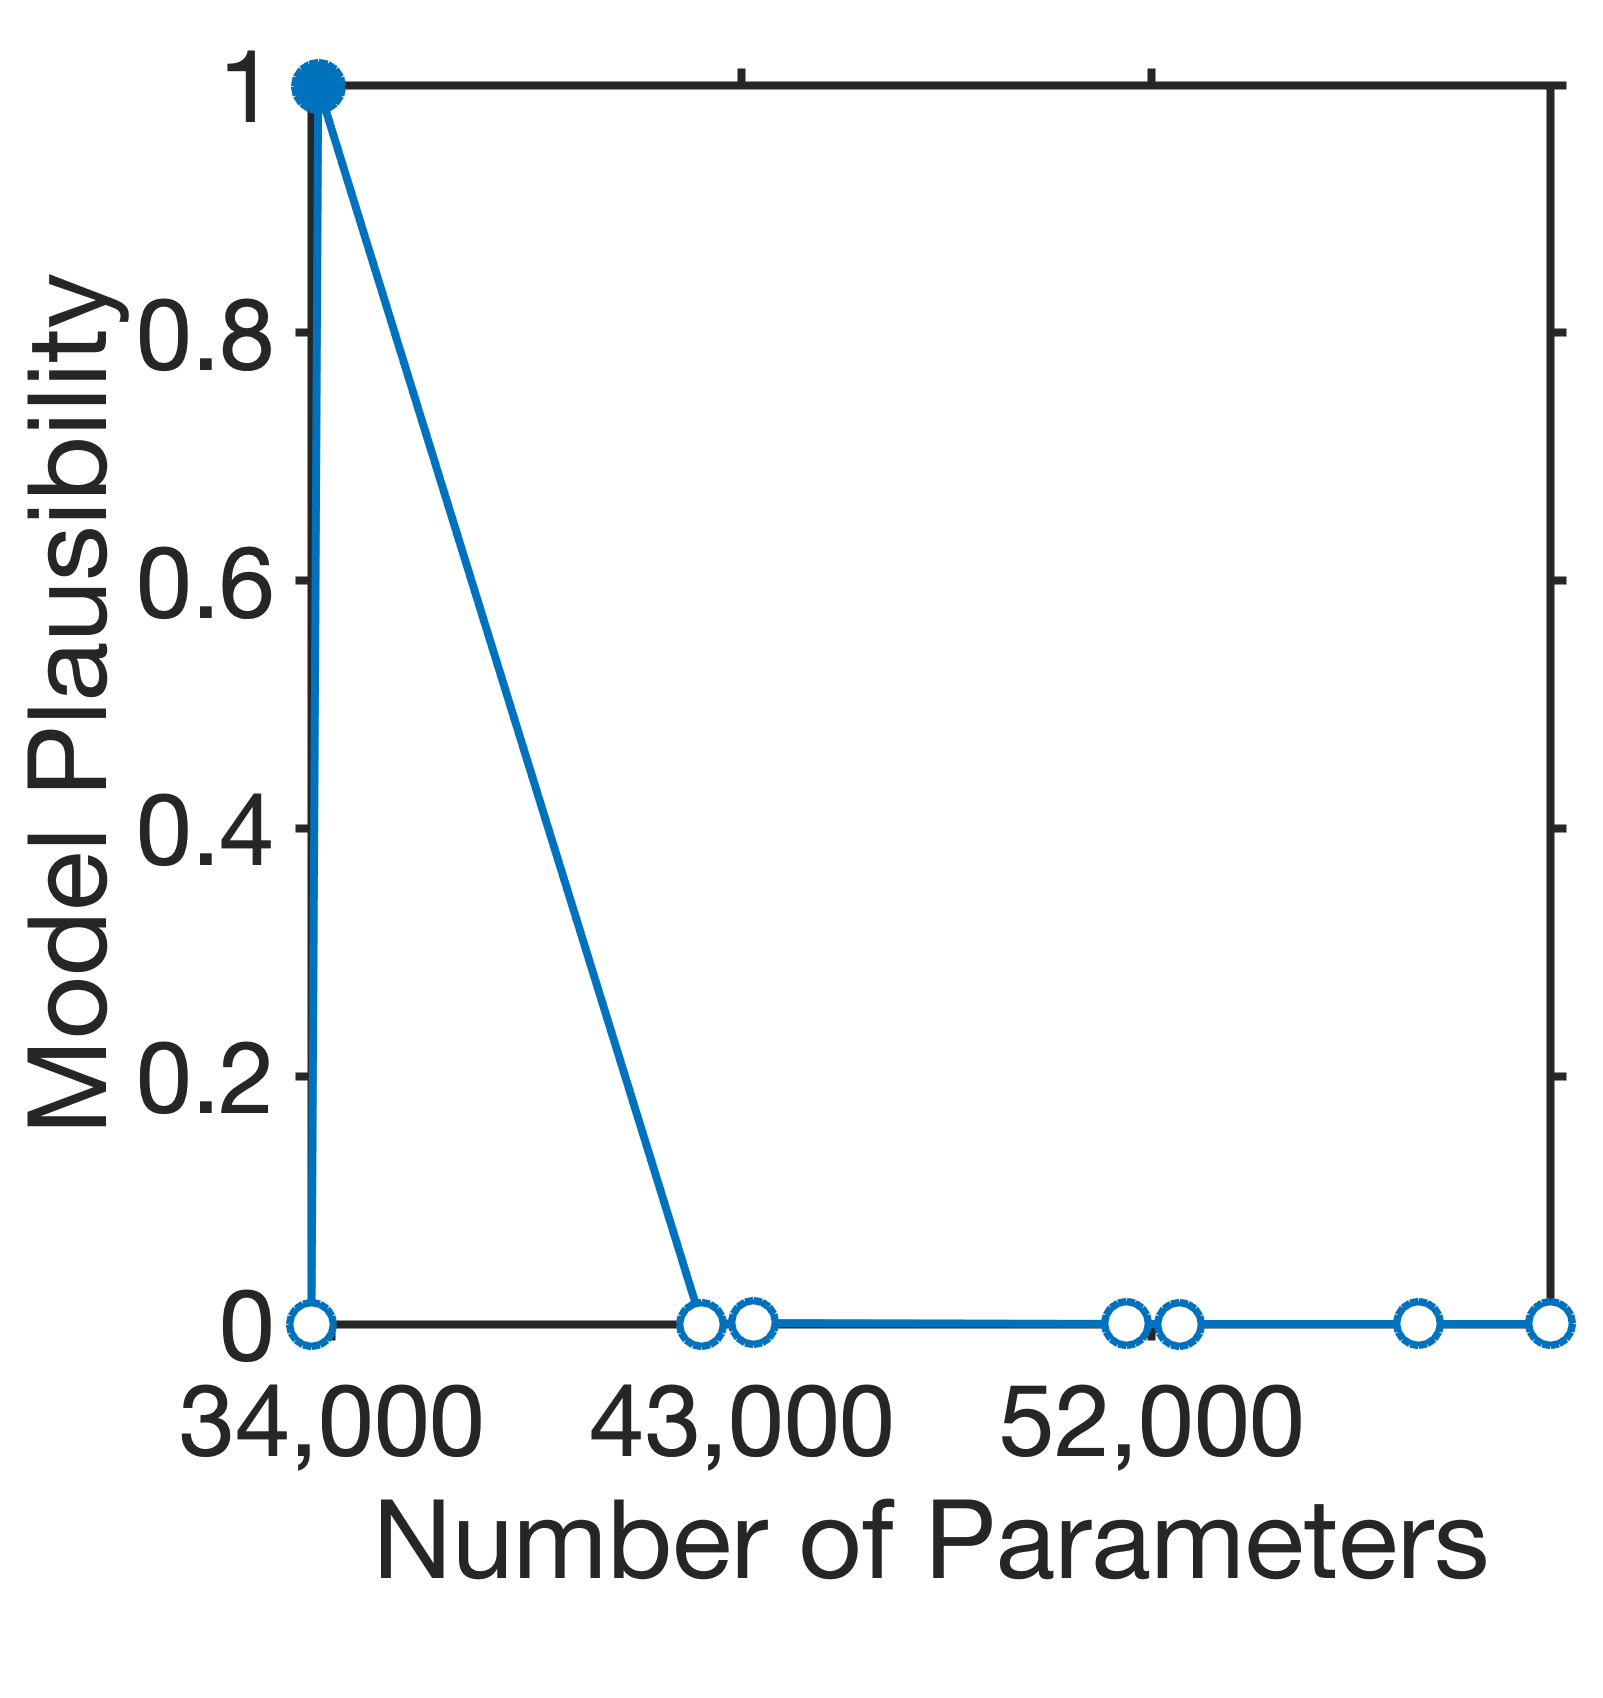
\includegraphics[width=0.19\textwidth]{Figures/Part B/cat2/fold1.png}\hfill
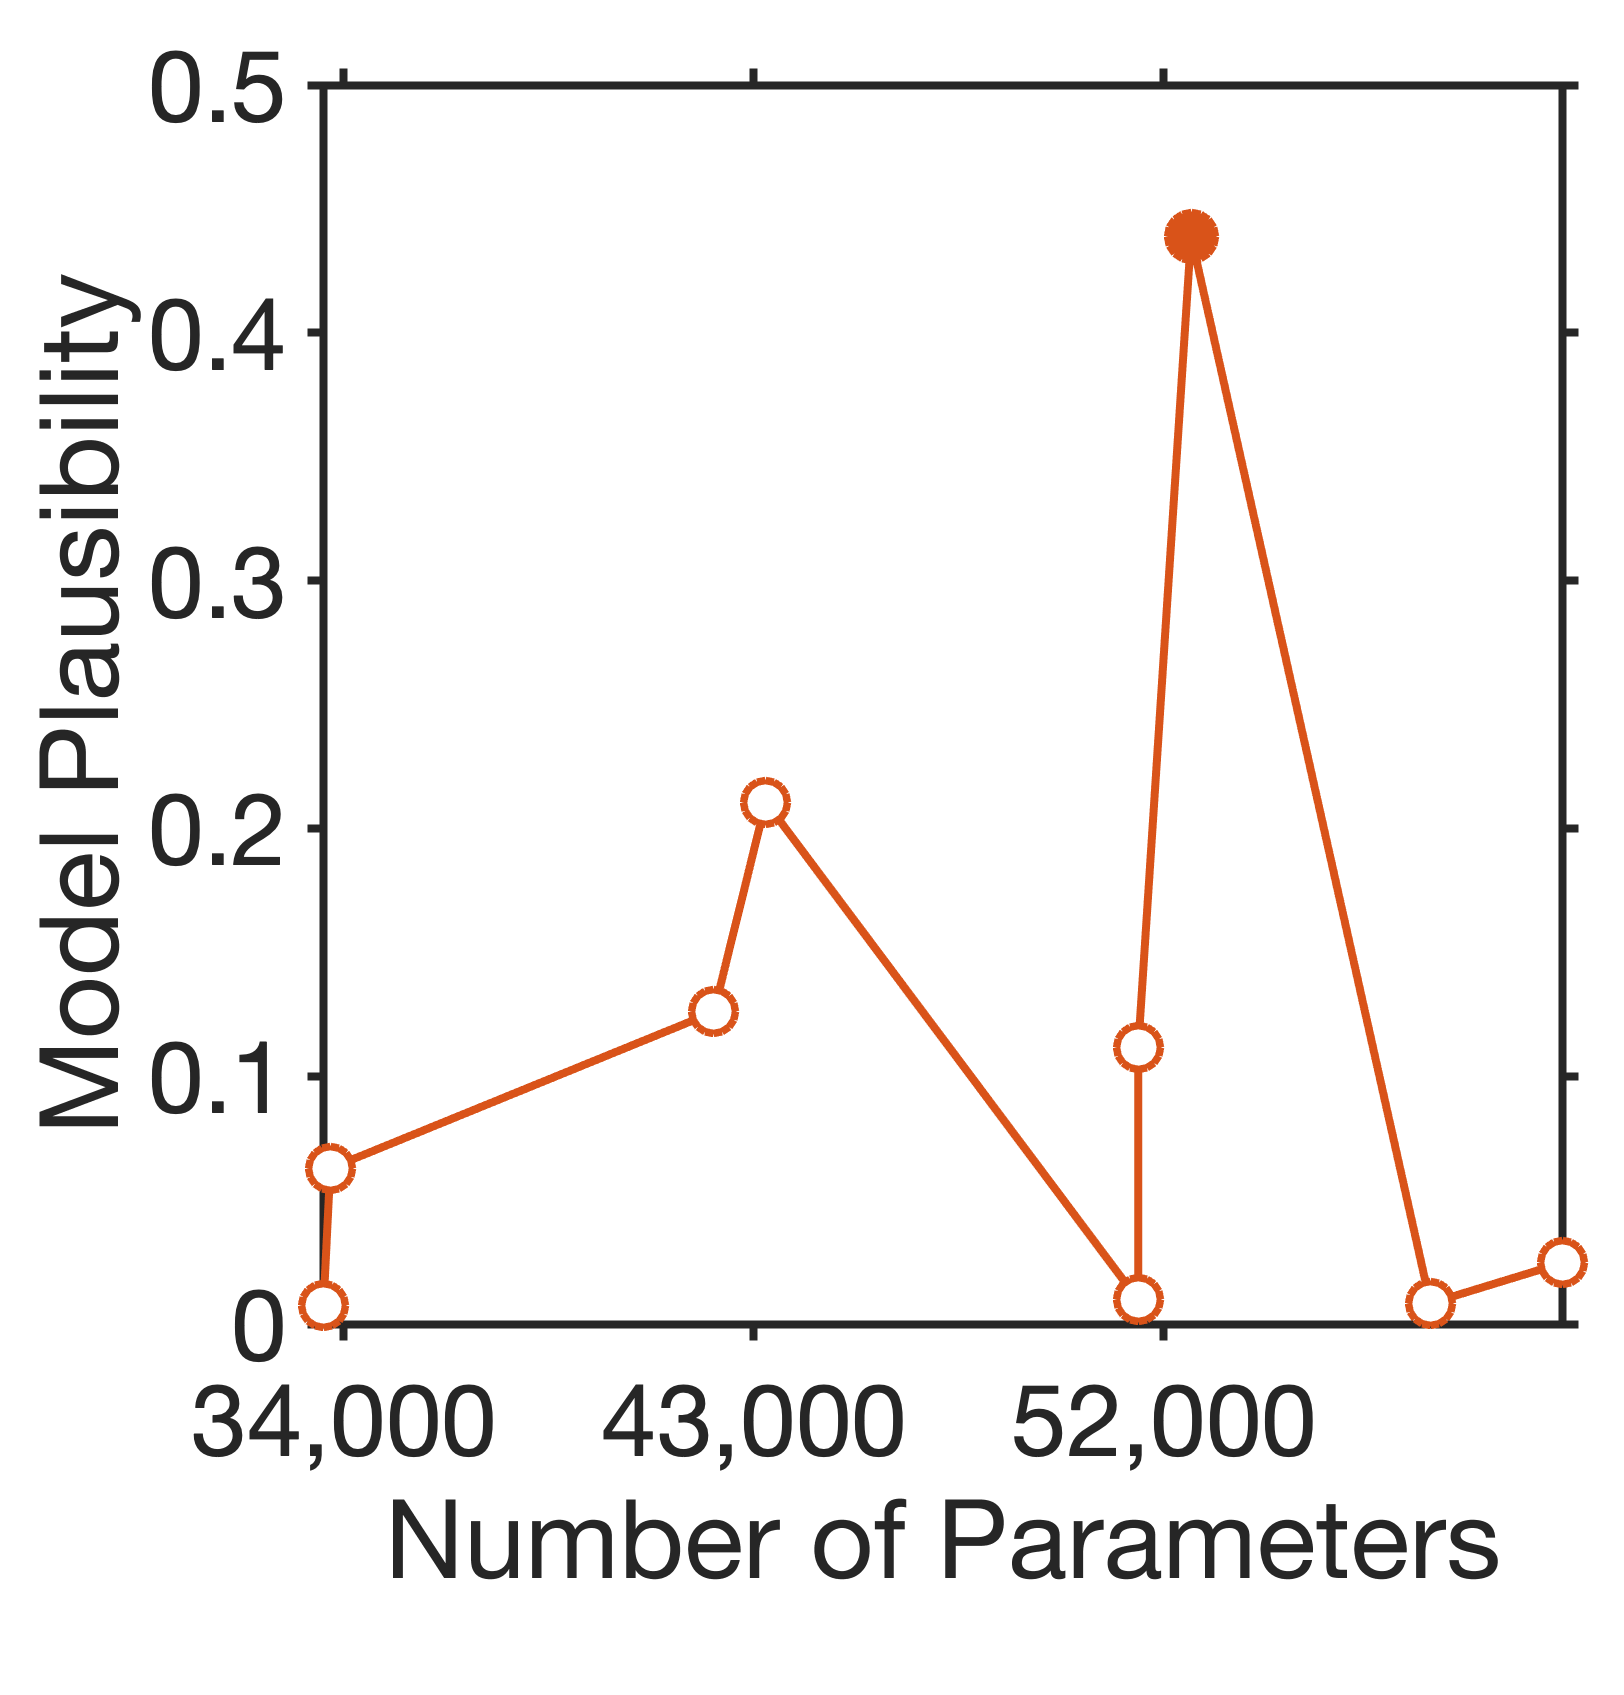
\includegraphics[width=0.19\textwidth]{Figures/Part B/cat2/fold2.png}\hfill
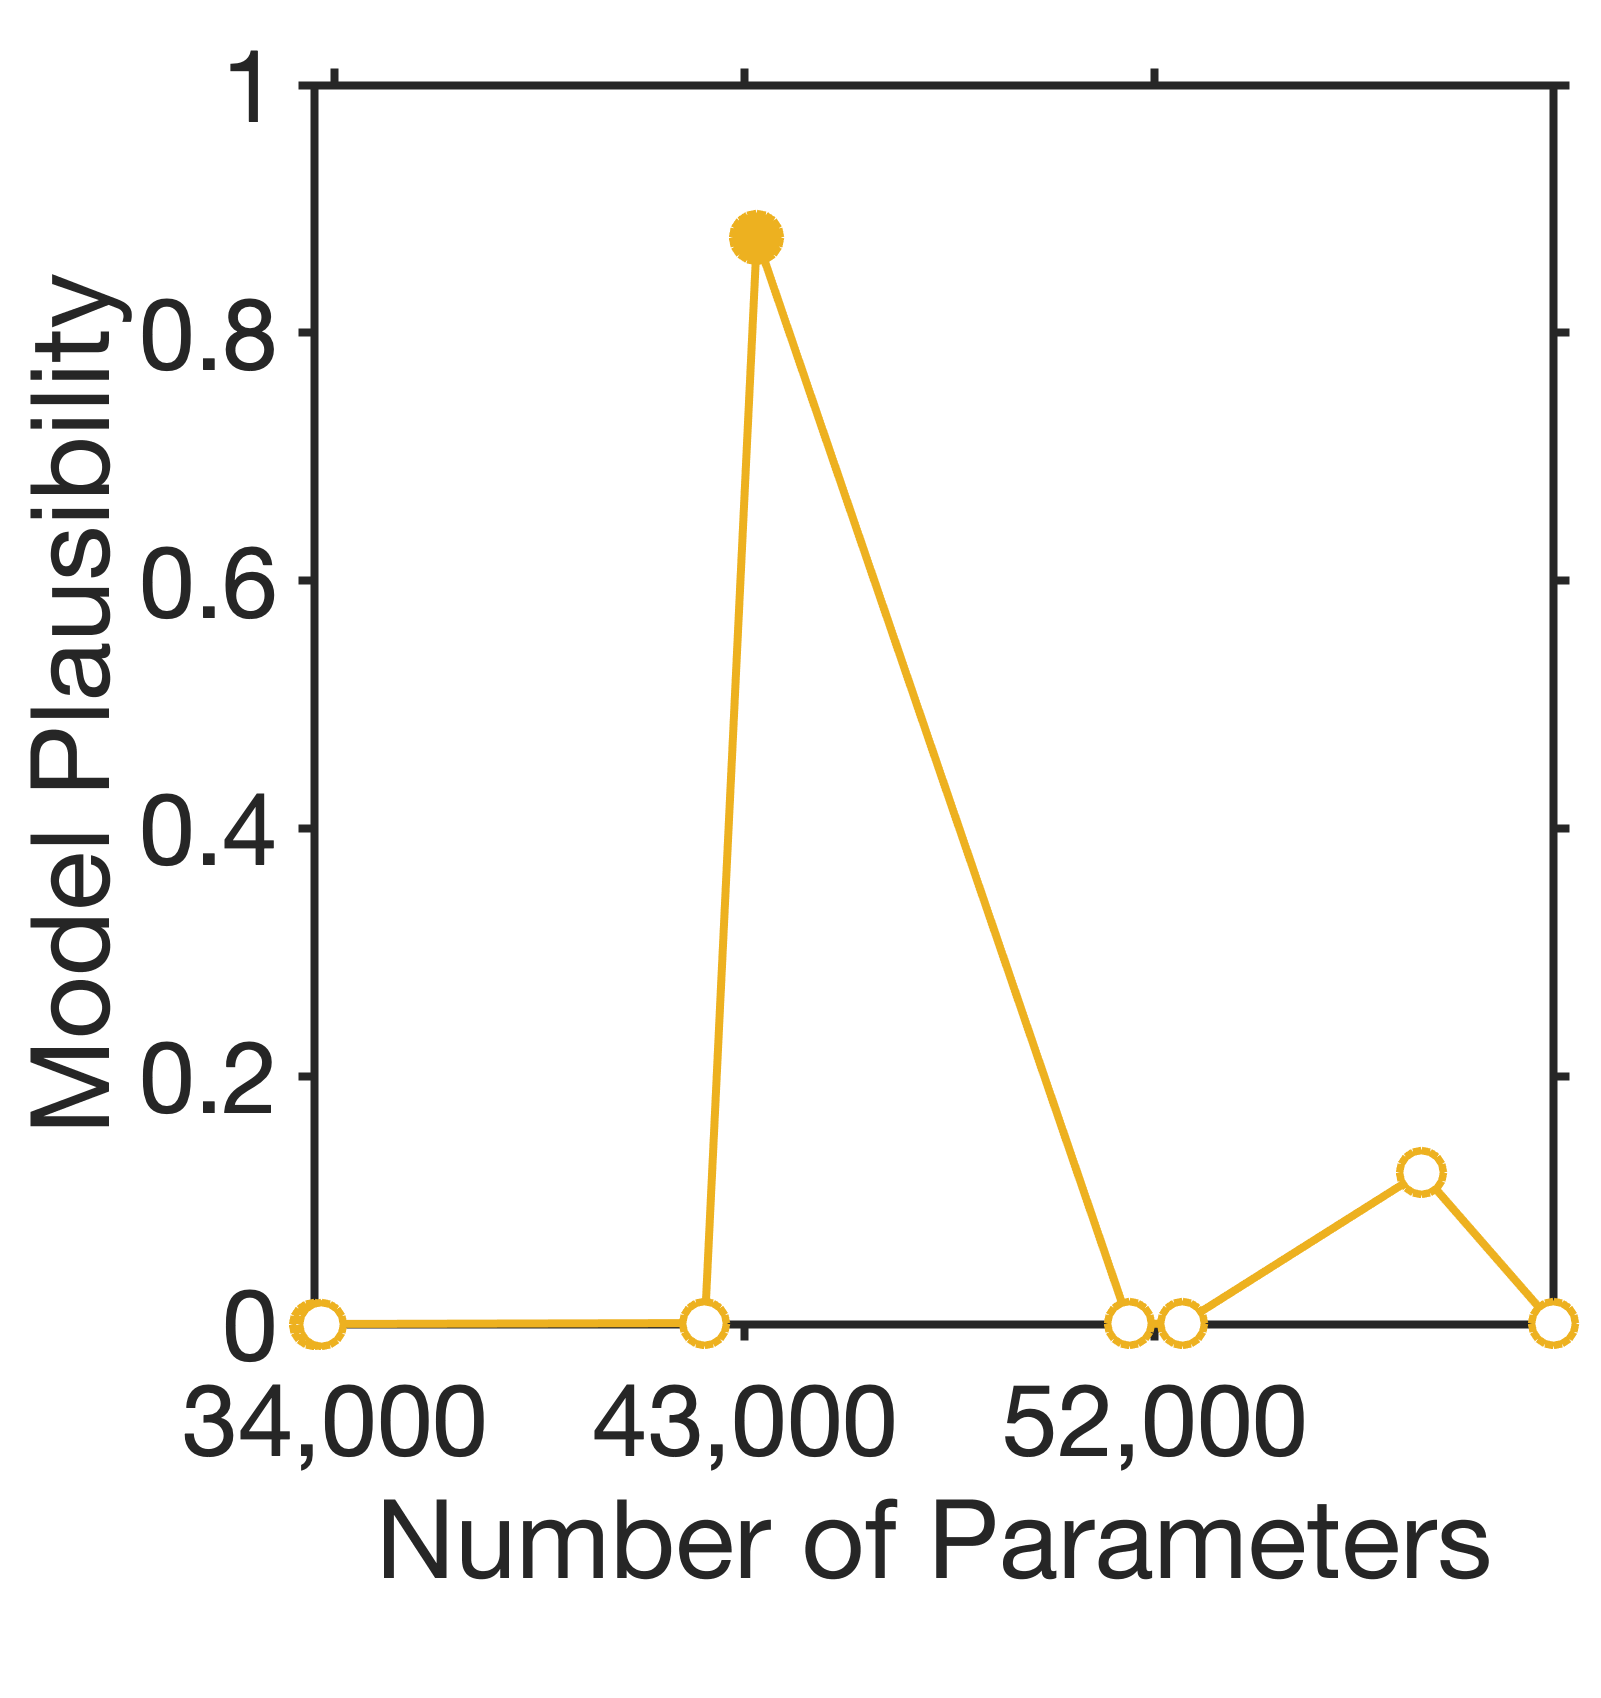
\includegraphics[width=0.19\textwidth]{Figures/Part B/cat2/fold3.png}\hfill
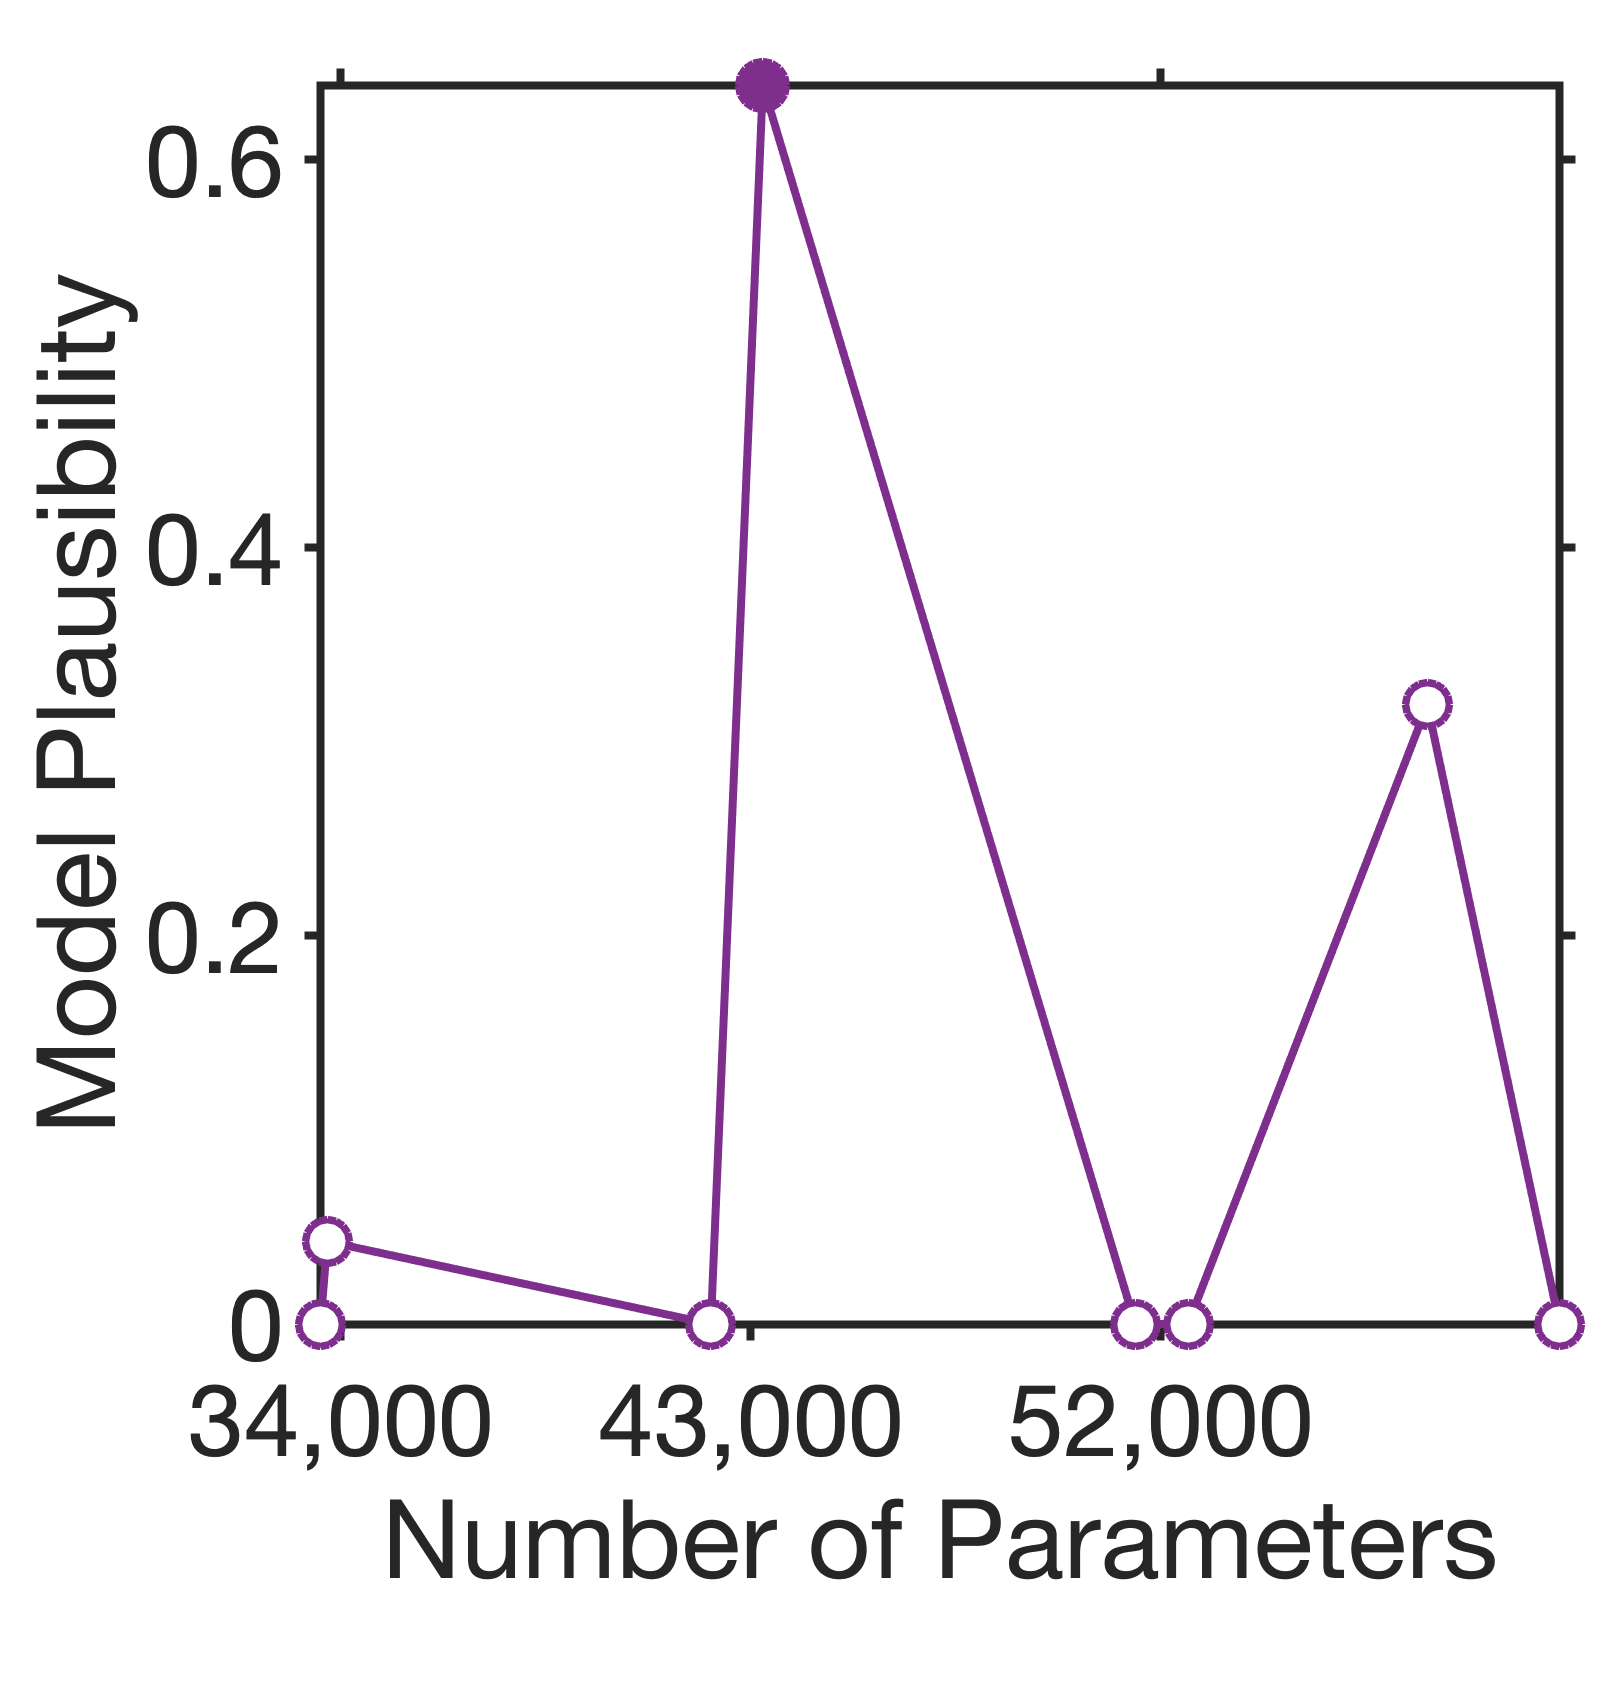
\includegraphics[width=0.19\textwidth]{Figures/Part B/cat2/fold4.png}\hfill
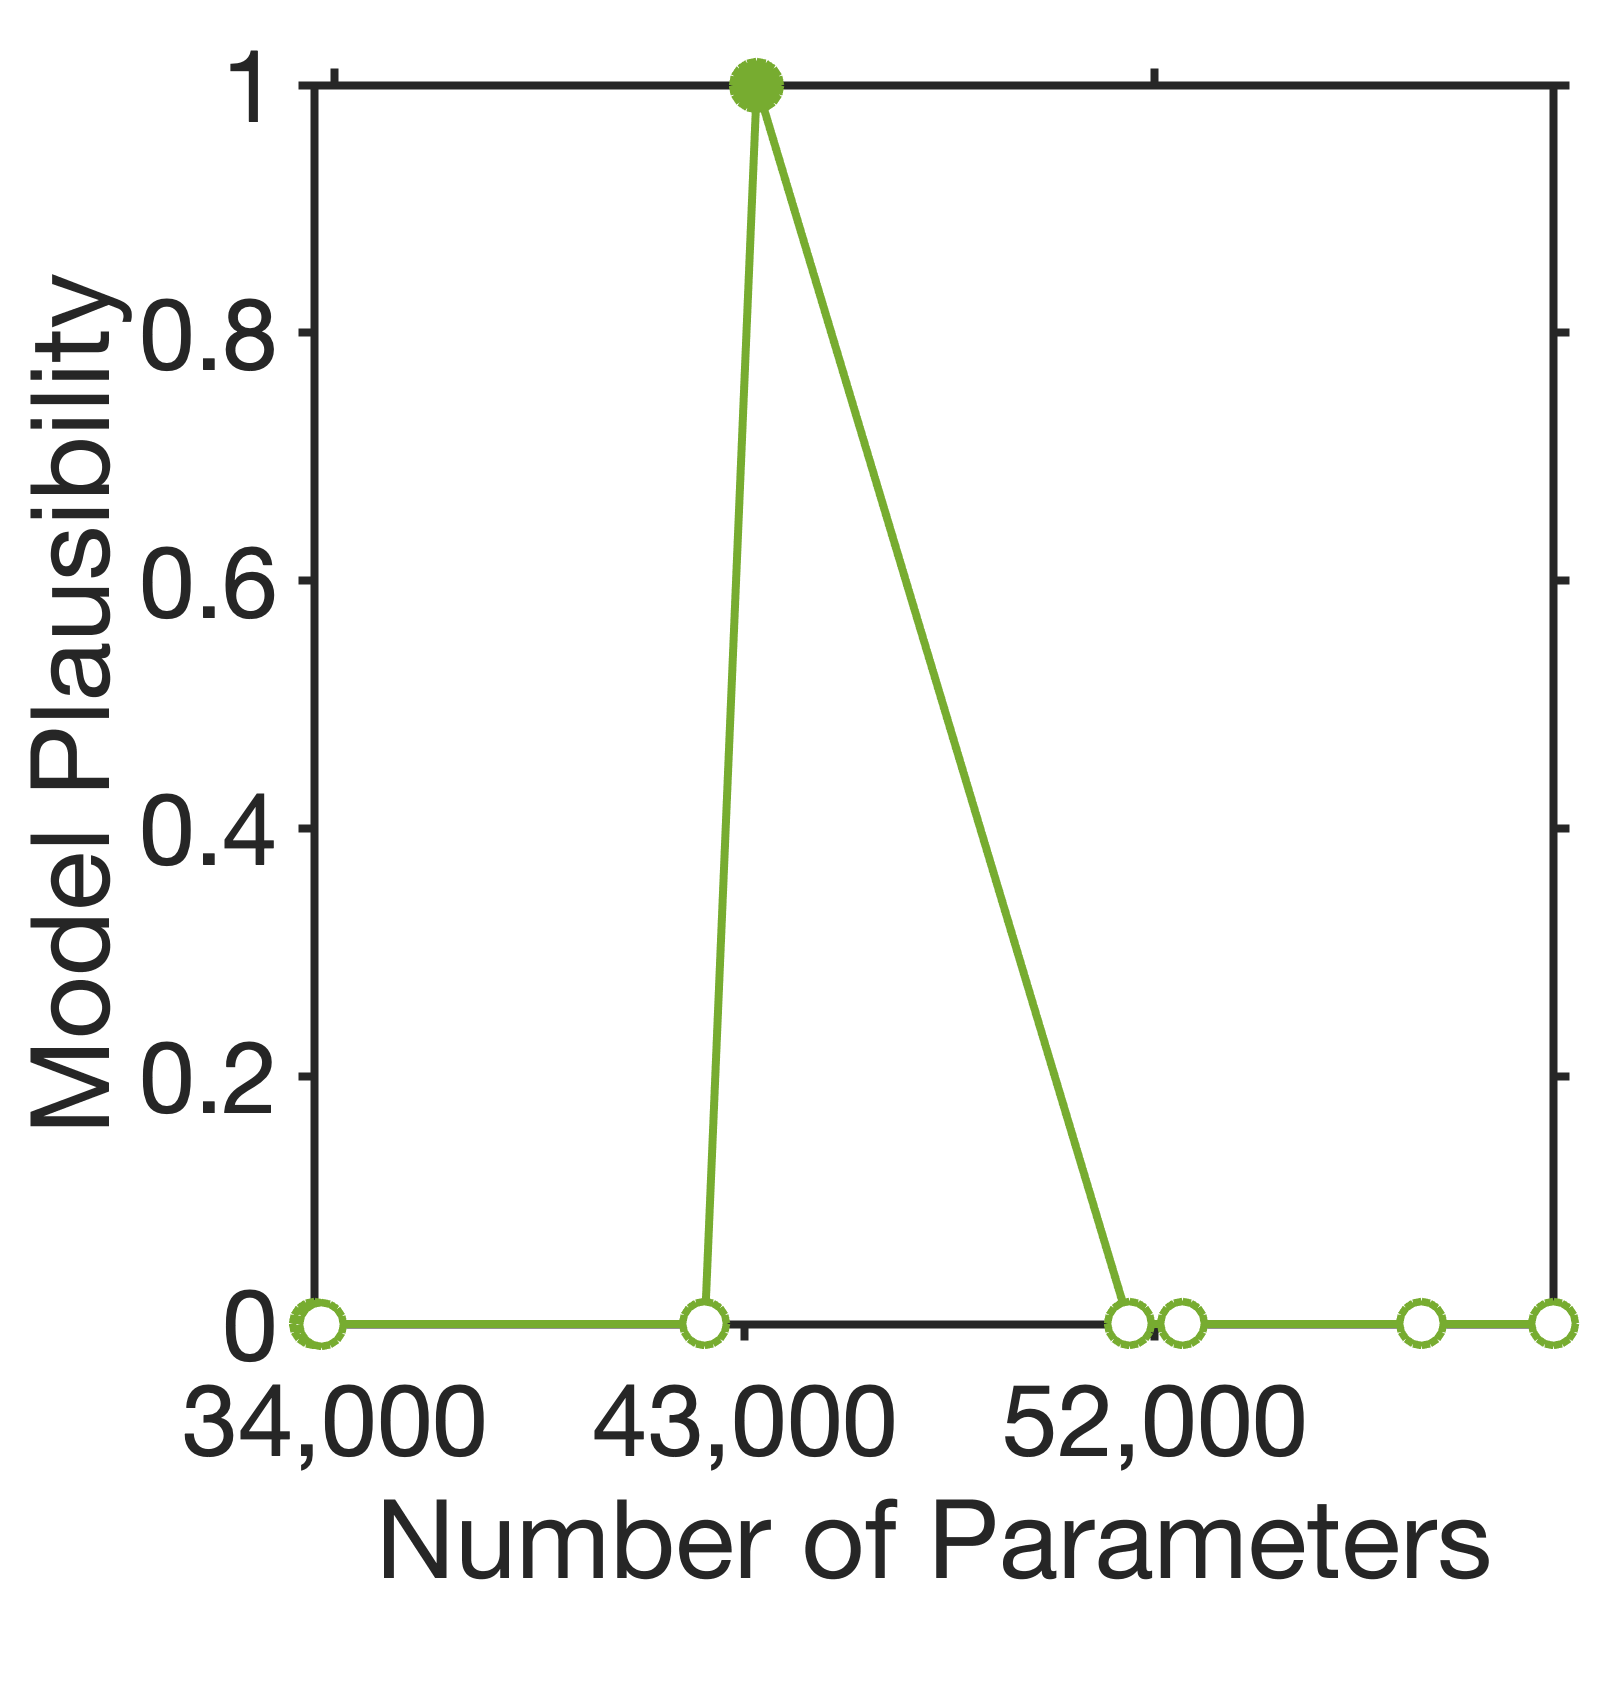
\includegraphics[width=0.19\textwidth]{Figures/Part B/cat2/fold5.png}

\caption{Model Plausibility plotted against number of parameters for all folds in category 2 (from Lett to right: fold 1 to fold 5 respectively)}
\label{fig:cat2-plausibility}
\end{figure}


\begin{figure}[H]
\centering

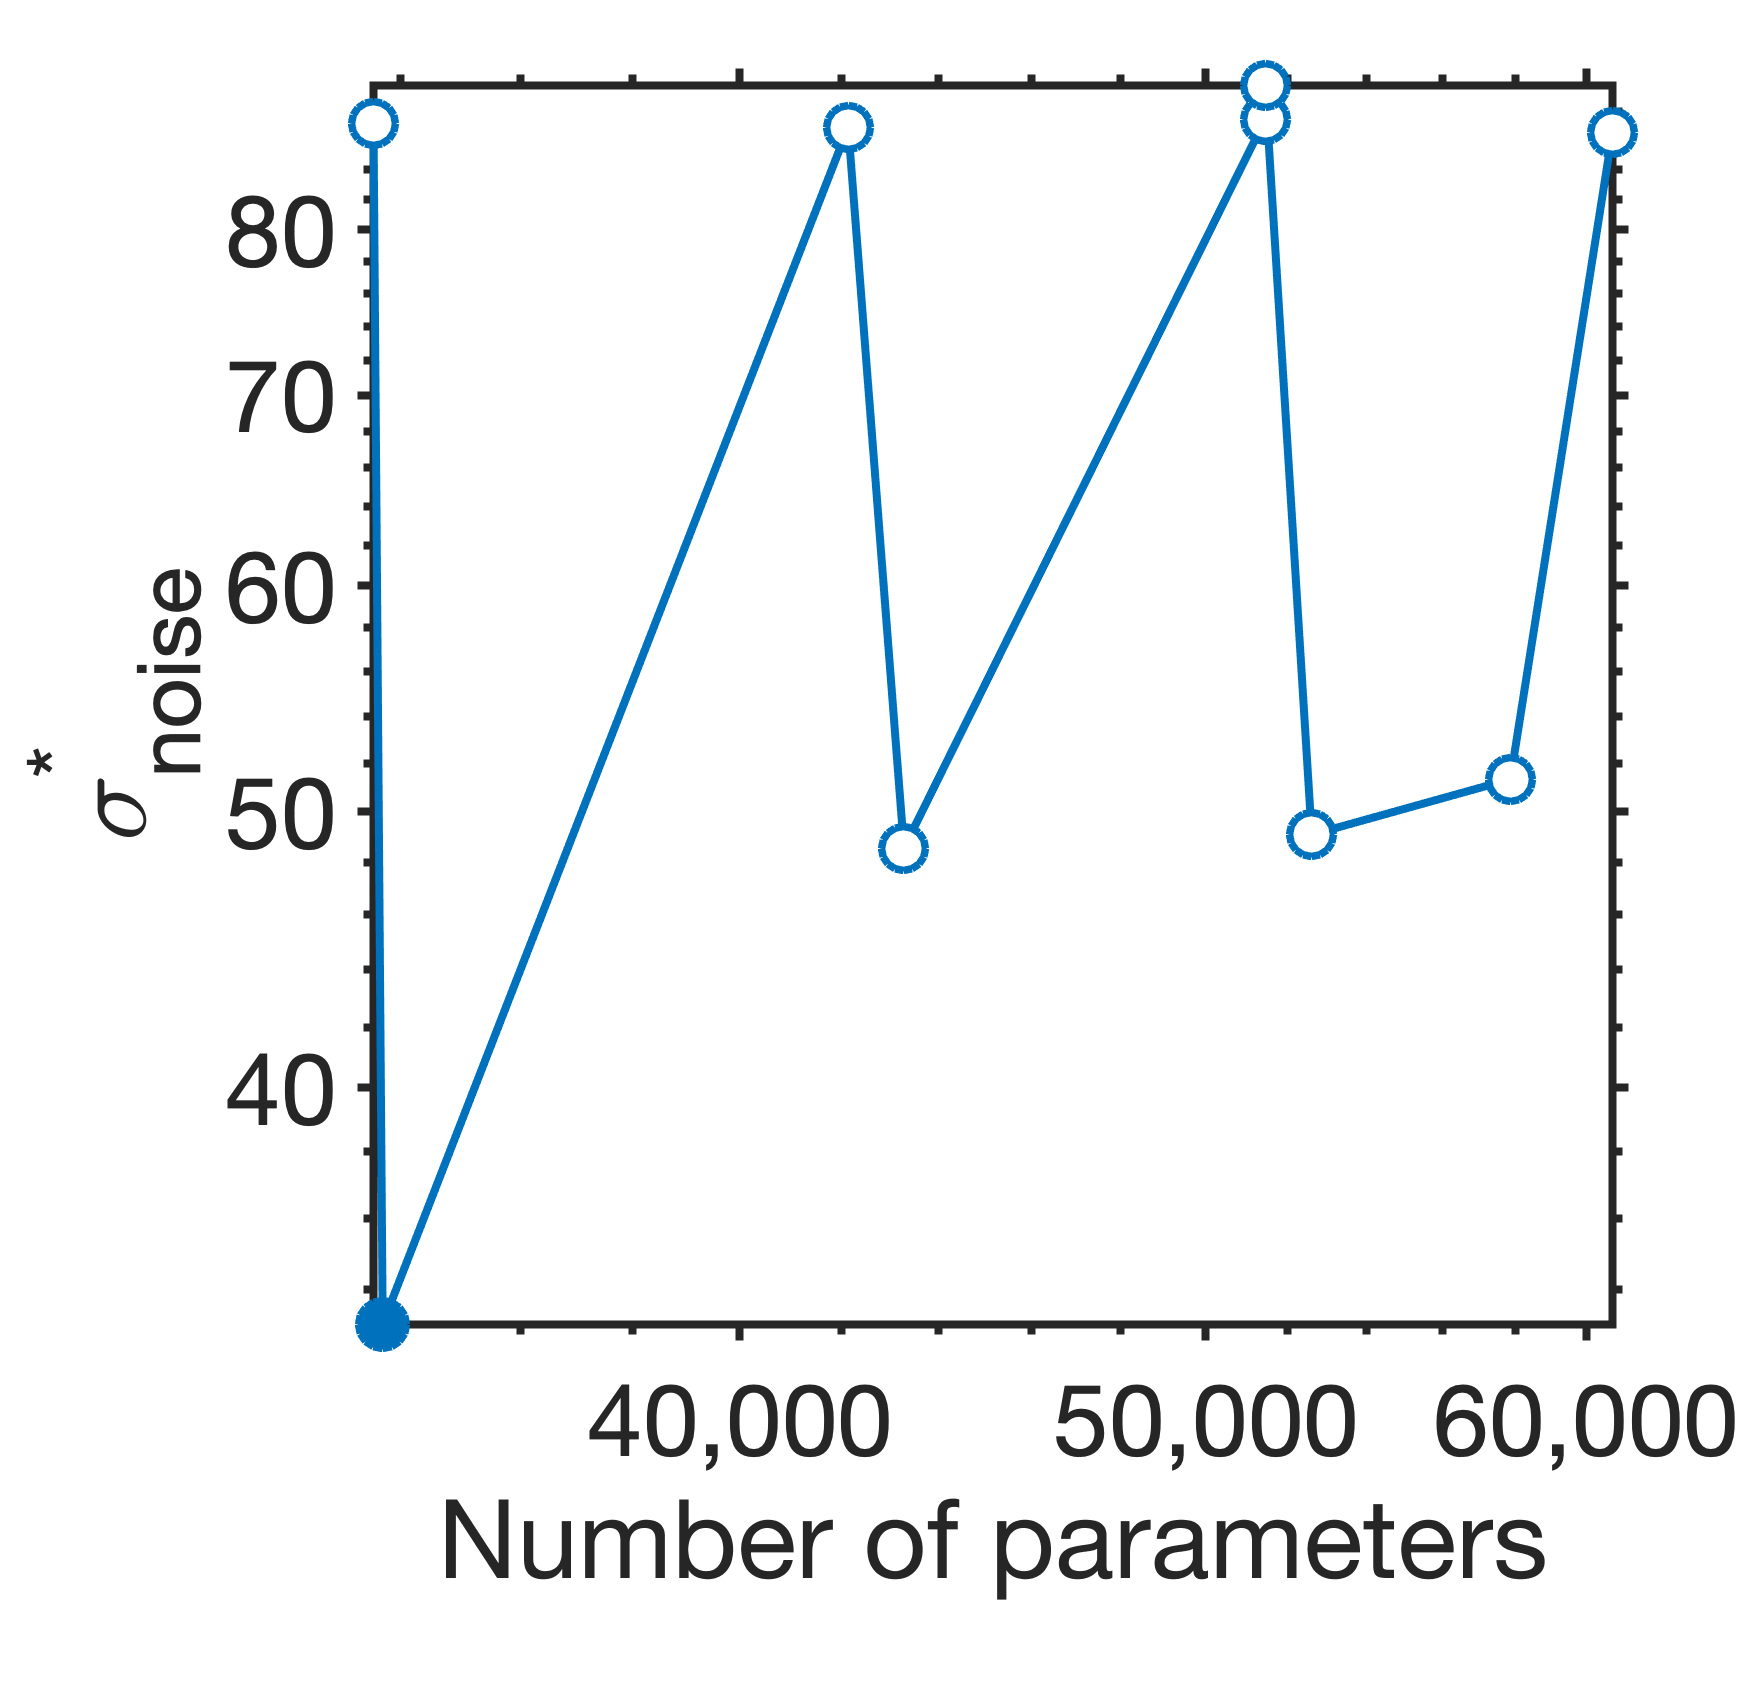
\includegraphics[width=0.19\textwidth]{Figures/Part B/cat2/fold1_noise.png}\hfill
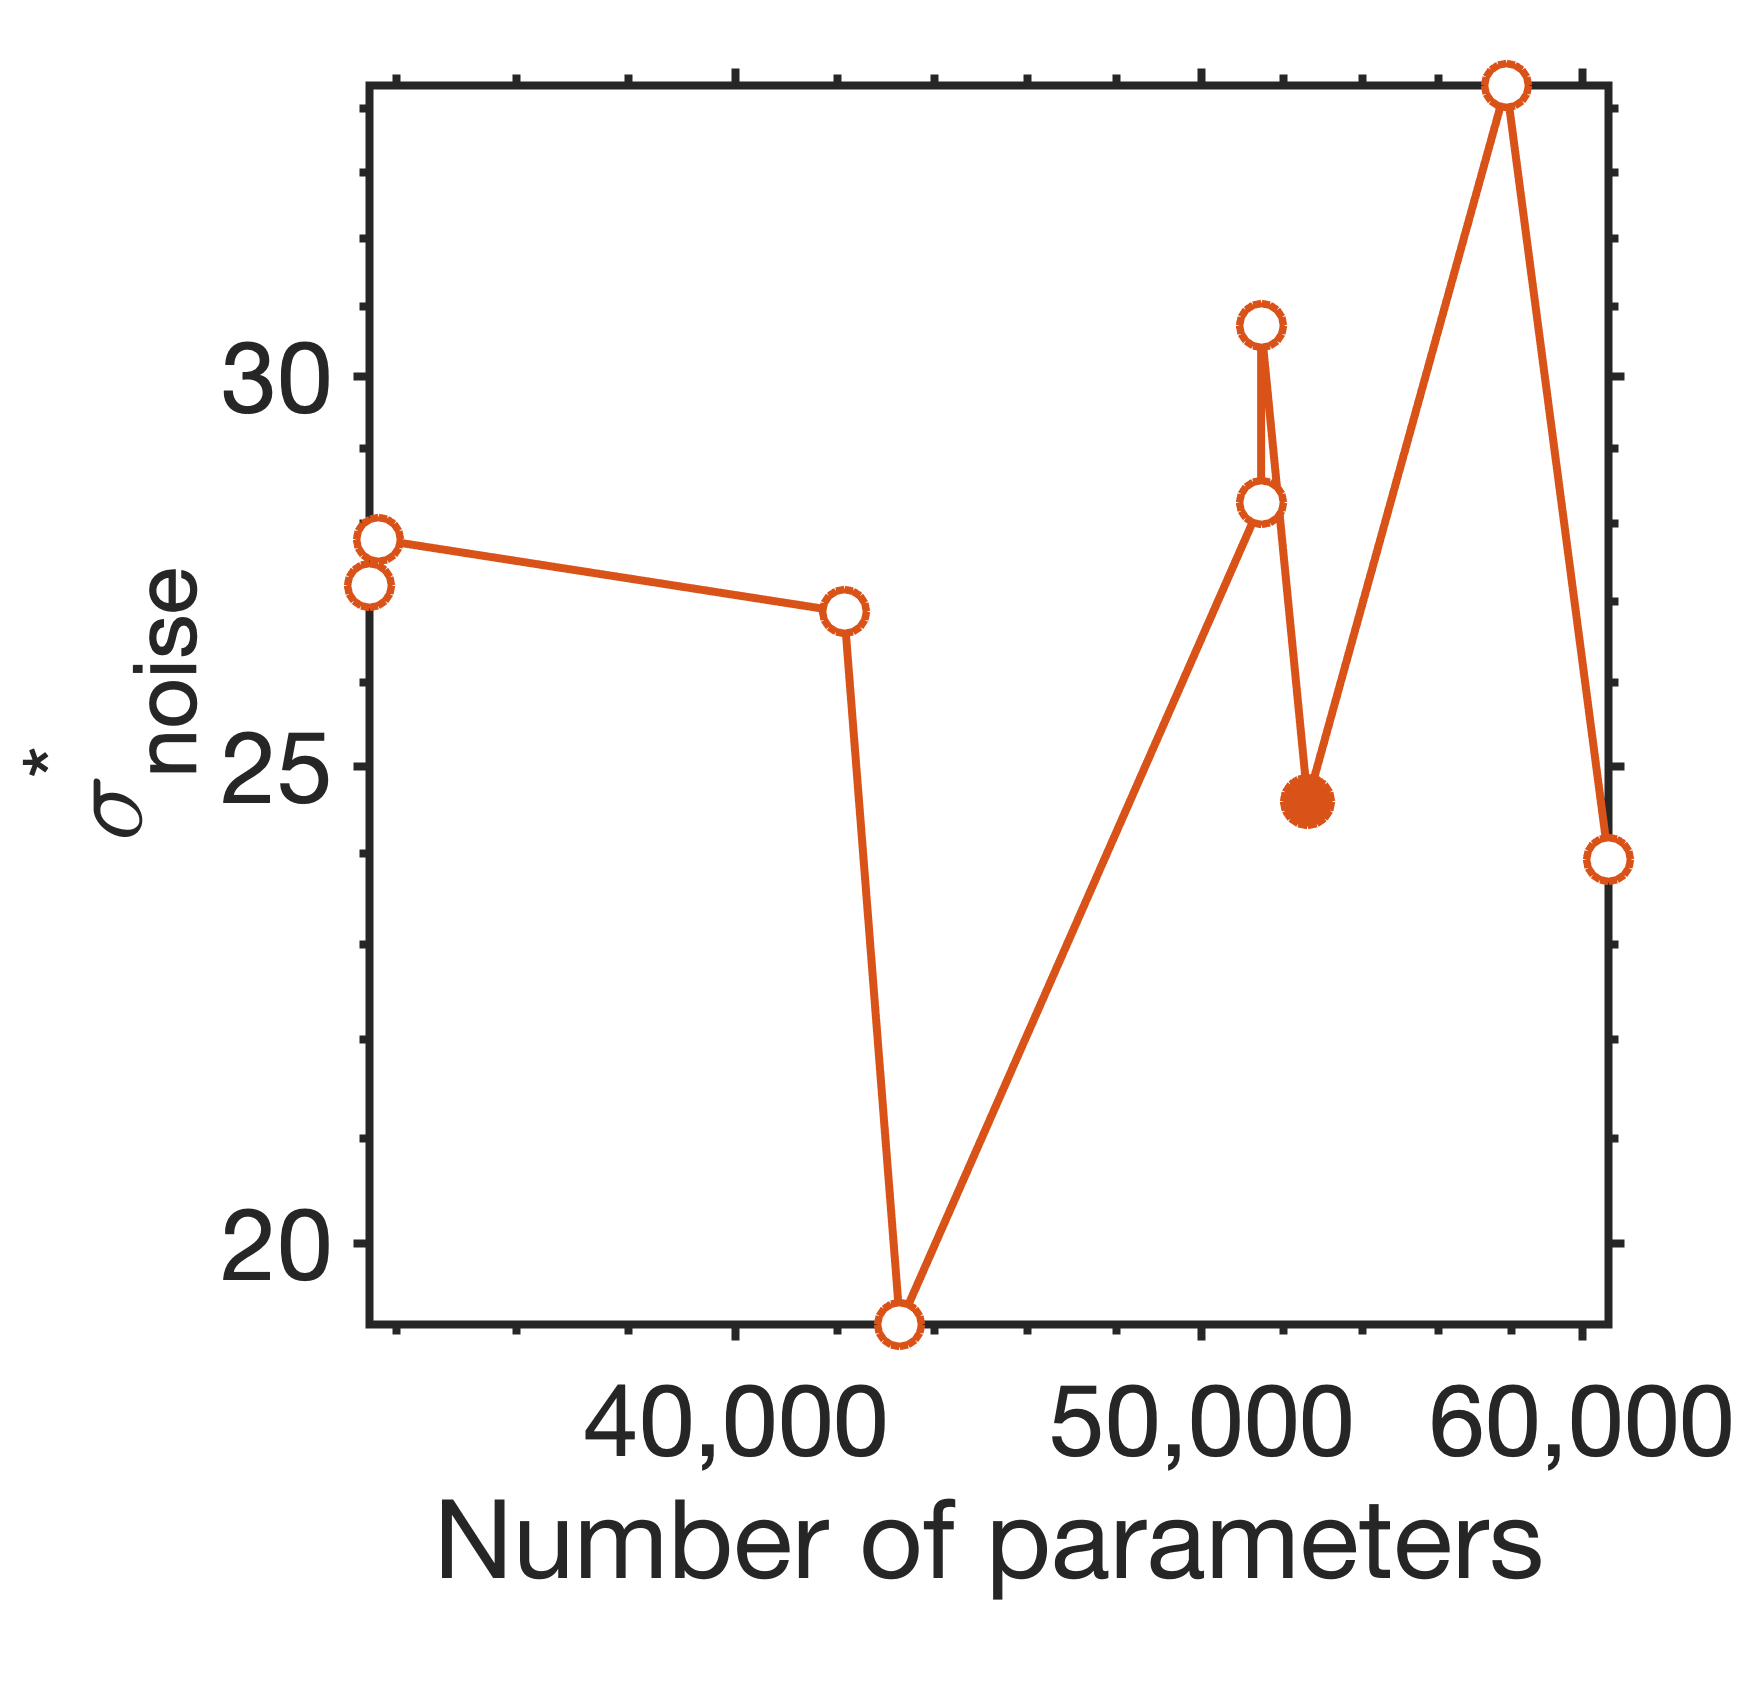
\includegraphics[width=0.19\textwidth]{Figures/Part B/cat2/fold2_noise.png}\hfill
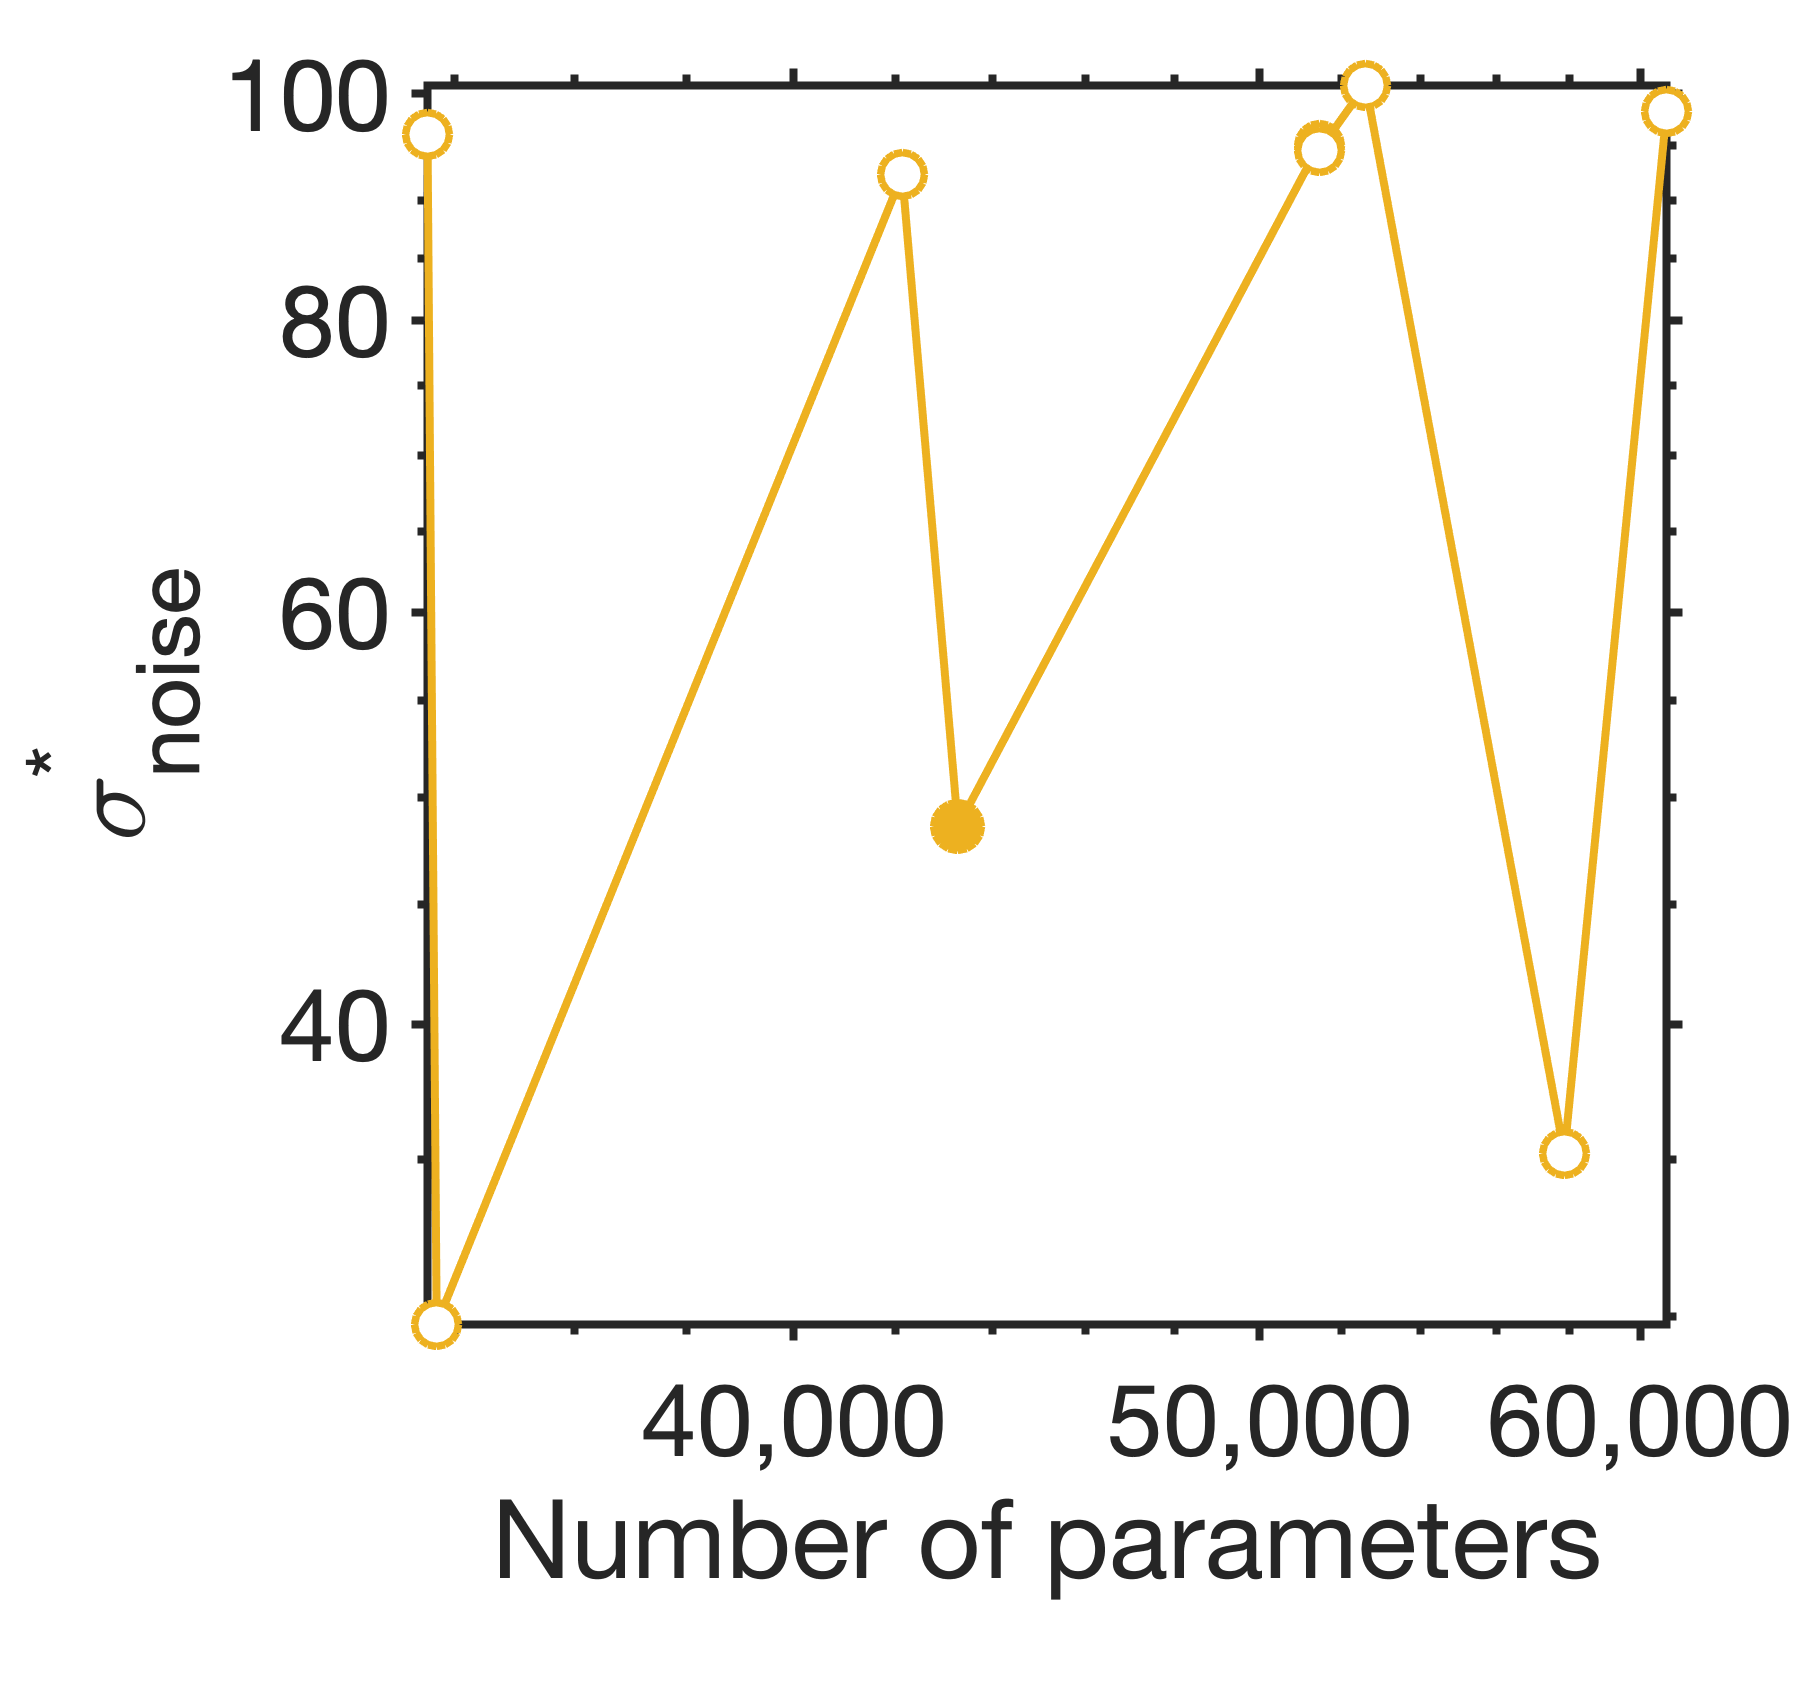
\includegraphics[width=0.19\textwidth]{Figures/Part B/cat2/fold3_noise.png}\hfill
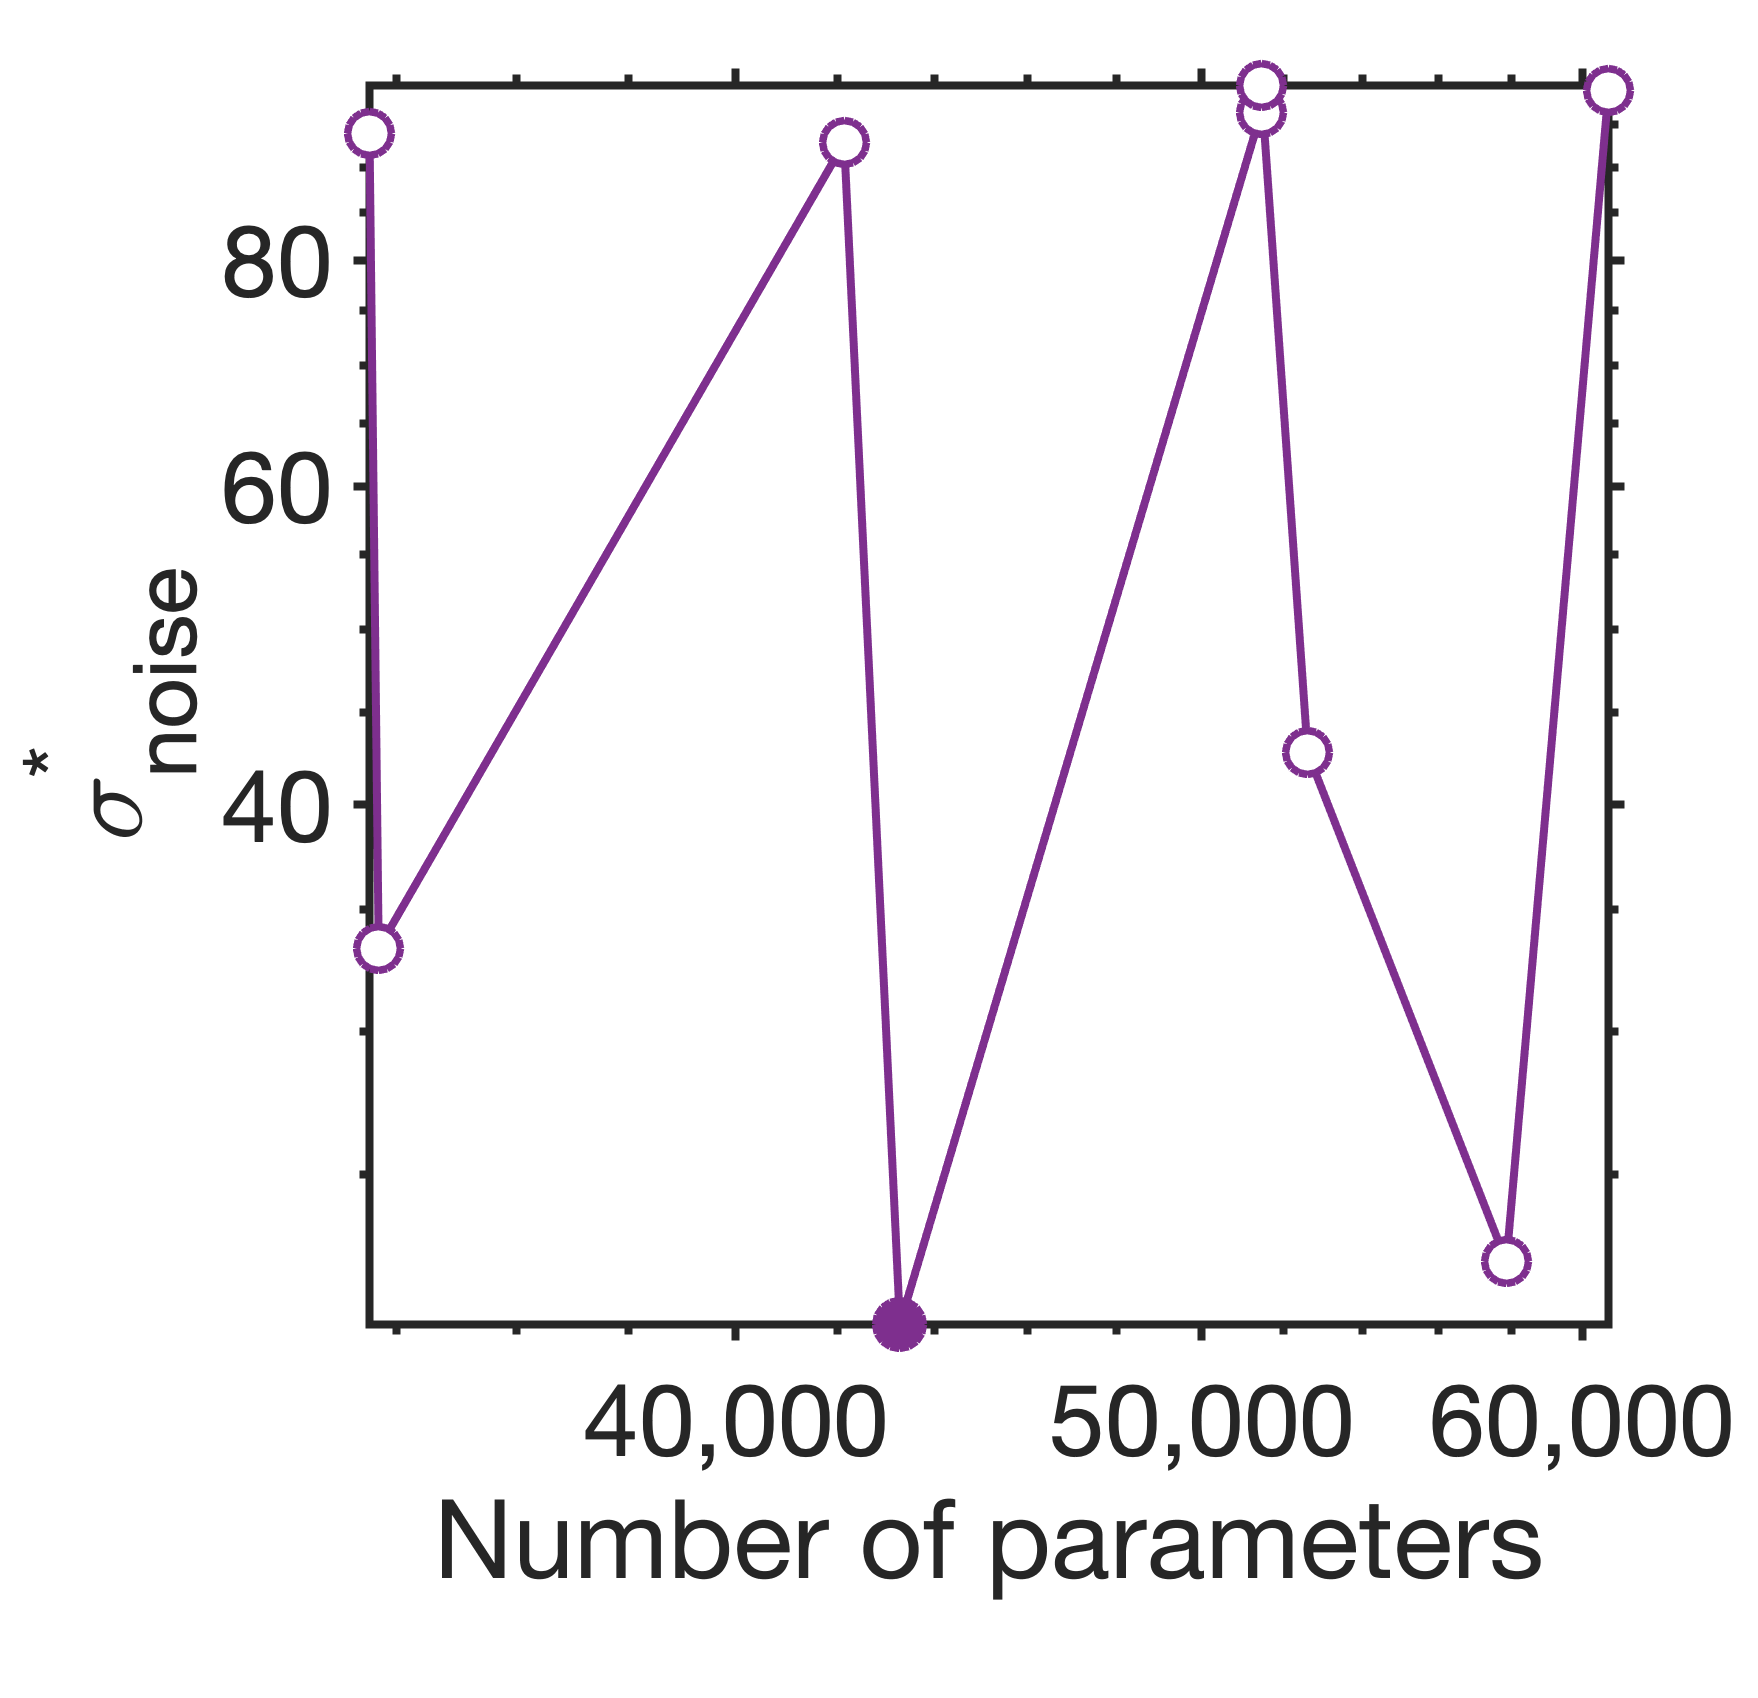
\includegraphics[width=0.19\textwidth]{Figures/Part B/cat2/fold4_noise.png}\hfill
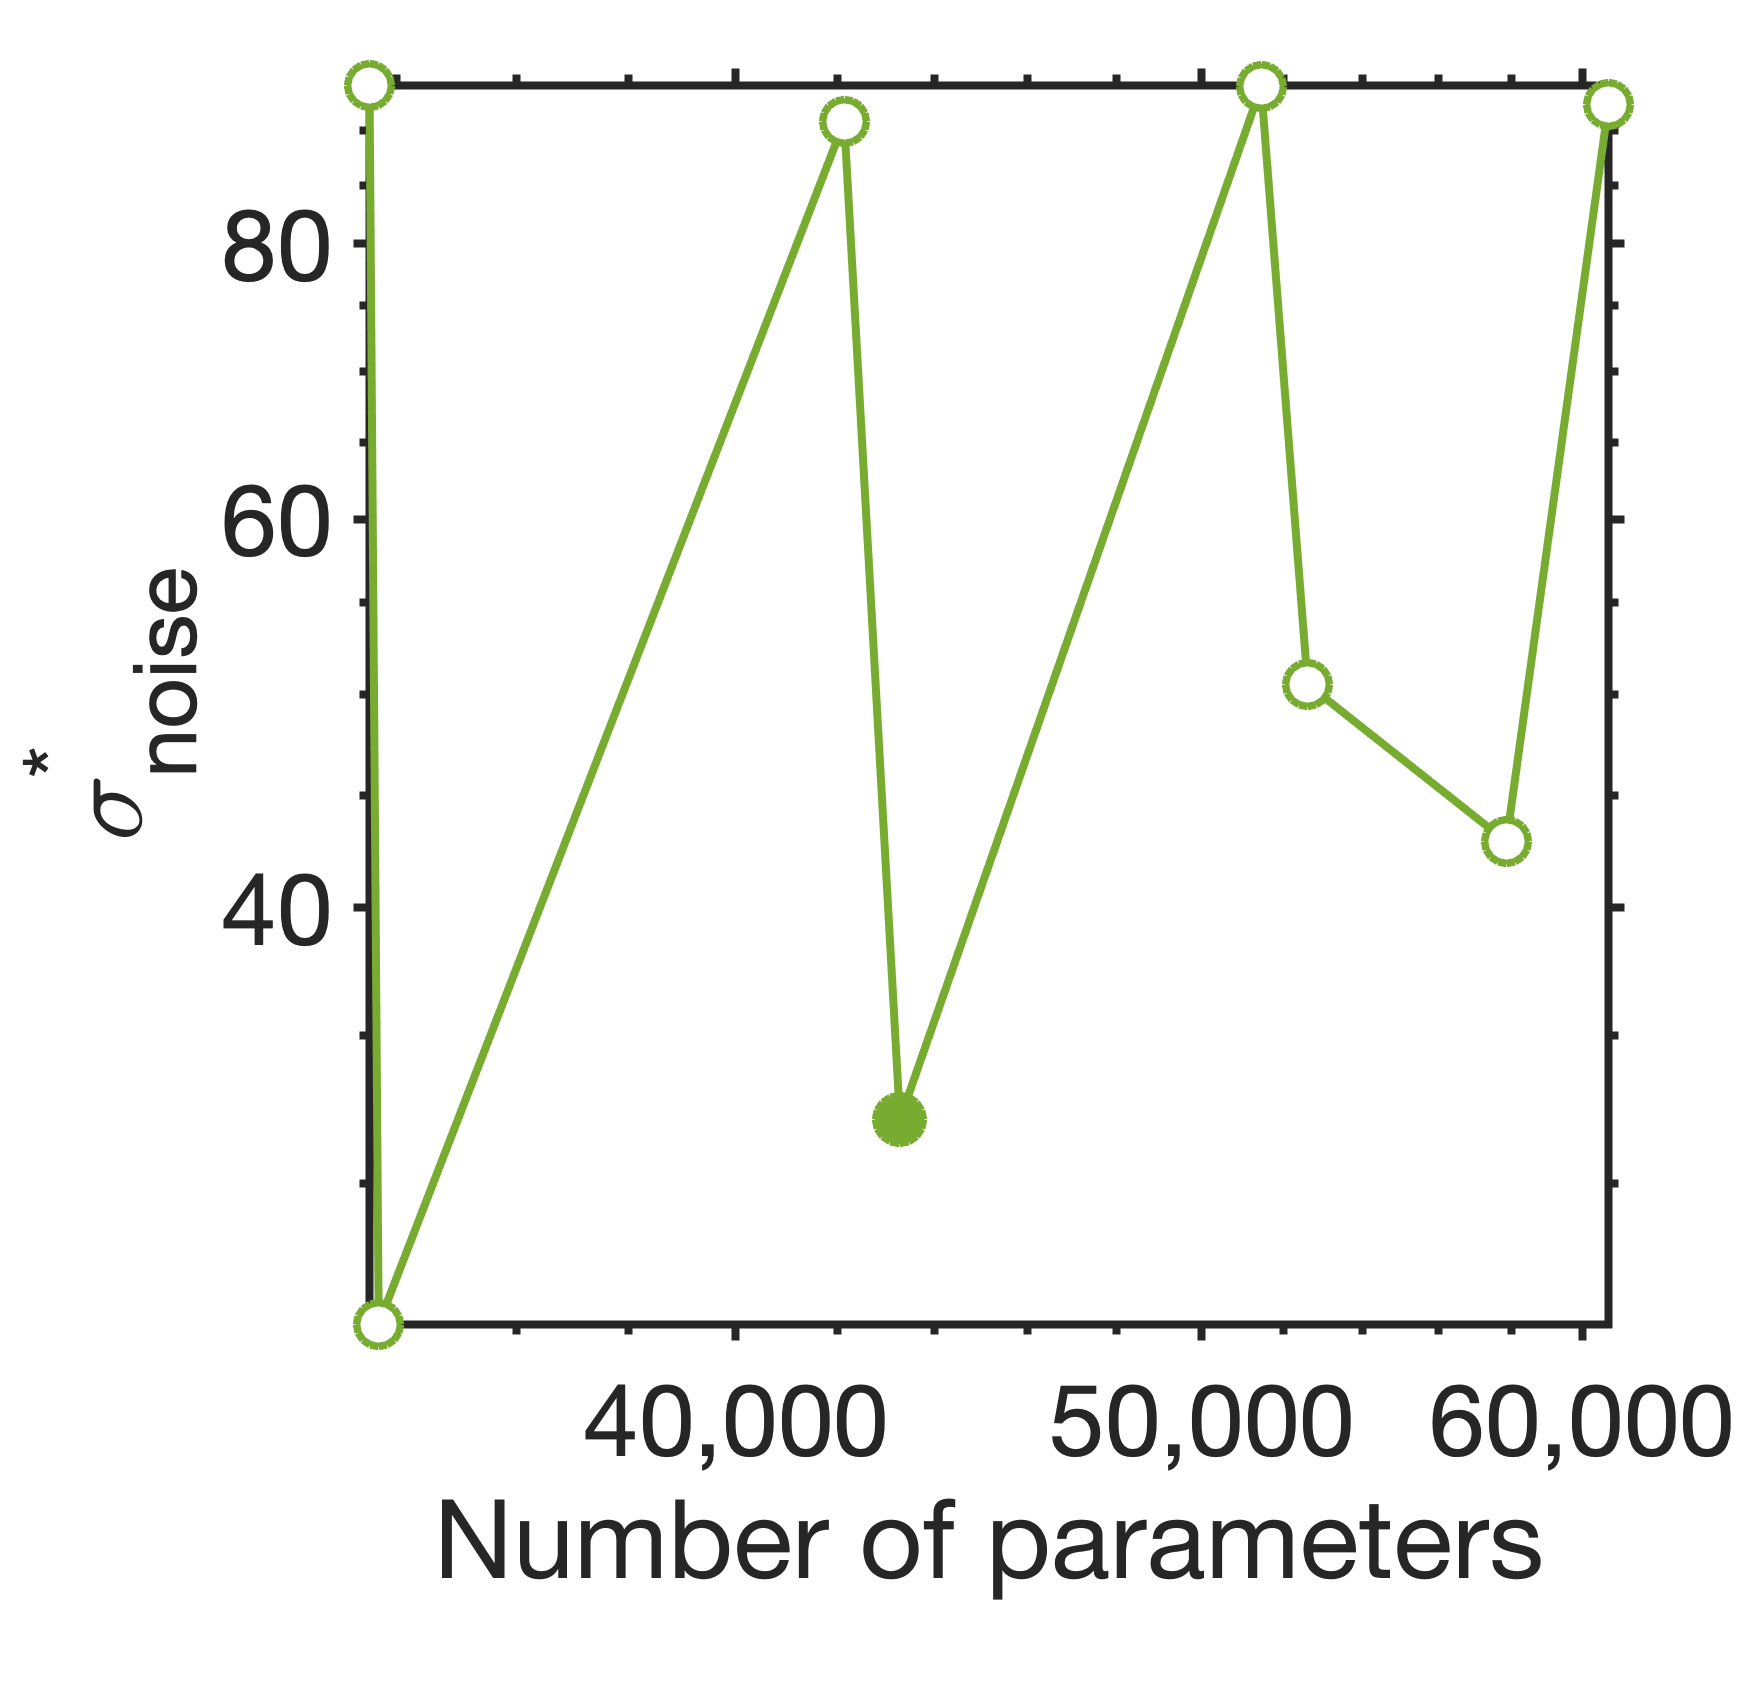
\includegraphics[width=0.19\textwidth]{Figures/Part B/cat2/fold5_noise.png}

\caption{Optimum $\sigma_{noise} $ plotted against number of parameters for different folds in category 2 (from Lett to right: fold 1 to fold 5 respectively)}
\label{fig:cat2_sigma}
\end{figure}

\autoref{fig:cat2-plausibility} and \autoref{fig:cat2_sigma} show, for each cross-validation fold (left-to-right: folds~1--5), how model plausibility and the MAP-estimated $\sigma_{\text{noise}}$ change with parameter count within Category~2. The most plausible architecture changes across folds because each fold’s training cohort has a different statistical profile, mainly due to inter-patient heterogeneity in glucose dynamics. Across the ten subjects, most patients have mean glucose in the 173–285 mg/dL range. Patient 7 is a clear outlier (mean 440 mg/dL, peak 769 mg/dL), and Patient 5 is moderately elevated (mean 285 mg/dL, peak 460 mg/dL). Patient 7 is withheld from fold 2 in validation, making the training cohort substantially more homogeneous. So, the evidence can justify a slightly more "long-range" design with fewer temporal blocks but wider channels, encoder $[4,8,16,32]$-decoder $[32,16,8,4]$. Using $d=4$ expands receptive field more aggressively per depth, while a larger kernel ($k=11$) provides a broader local context per convolution, which is beneficial when the training trajectories are more consistent. In contrast, folds whose training sets include more heterogeneous subjects prefer a denser coverage (smaller dilation base and/or more blocks). In Fold 1,3–5, the training set includes both Patients 7 and 5 along with six more moderate subjects, producing the largest variability in glucose magnitude. These folds prefer similar architecture with smaller kernel $k{=}9/7$ that limits the local temporal receptive window, providing more temporal resolution. The architectures have a dilation base of 3 with encoder $[2,4,8,16,32]$-decoder $[32,16,8,4,2]$ that builds the required receptive field gradually through additional depth rather than aggressive per-block expansion, giving the model more information to generalize over the heterogeneous glucose regime. 


Another key observation is that neither plausibility nor $\sigma_{\text{noise}}$ changes monotonically with the number of parameters. Instead, only a small subset of architectures with specific design achieves high plausibility. The $\sigma_{\text{noise}}$ trends suggest that architectures with poorer fit often (low plausibility) compensate by selecting larger $\sigma_{\text{noise}}$ (requiring more noise inflation to explain residual errors), while the higher plausible models typically require smaller $\sigma_{\text{noise}}$ across folds. 

This pattern of specific architectures is consistent with the validation plots. The \autoref{fig:cat2_success} panels show that Category 2 usually produces DT-usable TCN architectures. In their prediction plots the predictive mean follows meal responses and recovery, and the uncertainty bands remain in tolerable ranges. A limited number of failures still occur \autoref{fig:cat2_falied}, mainly around post-meal peaks. An architecture can be considered DT-reay if it passes any of the folds. Category~2 provides the most reliable DT-ready models overall. Most folds meet the validation requirement with credible uncertainty.


\begin{figure}[H]
\centering

\begin{minipage}[t]{0.48\textwidth}
  \centering
  \includegraphics[width=\linewidth]{Figures/Part B/cat2/p9_c2.png}
  \caption*{(a)}
\end{minipage}\hfill
\begin{minipage}[t]{0.48\textwidth}
  \centering
  \includegraphics[width=\linewidth]{Figures/Part B/cat2/p10_c2.png}
  \caption*{(b)}
\end{minipage}

\caption{(a) Patient 9 from fold 1, Architecture: $Cat_2Arch_2$, and (b) Patient 10 from fold 1, Architecture: $Cat_2Arch_2$.}
\label{fig:cat2_falied}
\end{figure}






\begin{figure}[H]
\centering

\begin{minipage}[t]{0.48\textwidth}
  \centering
  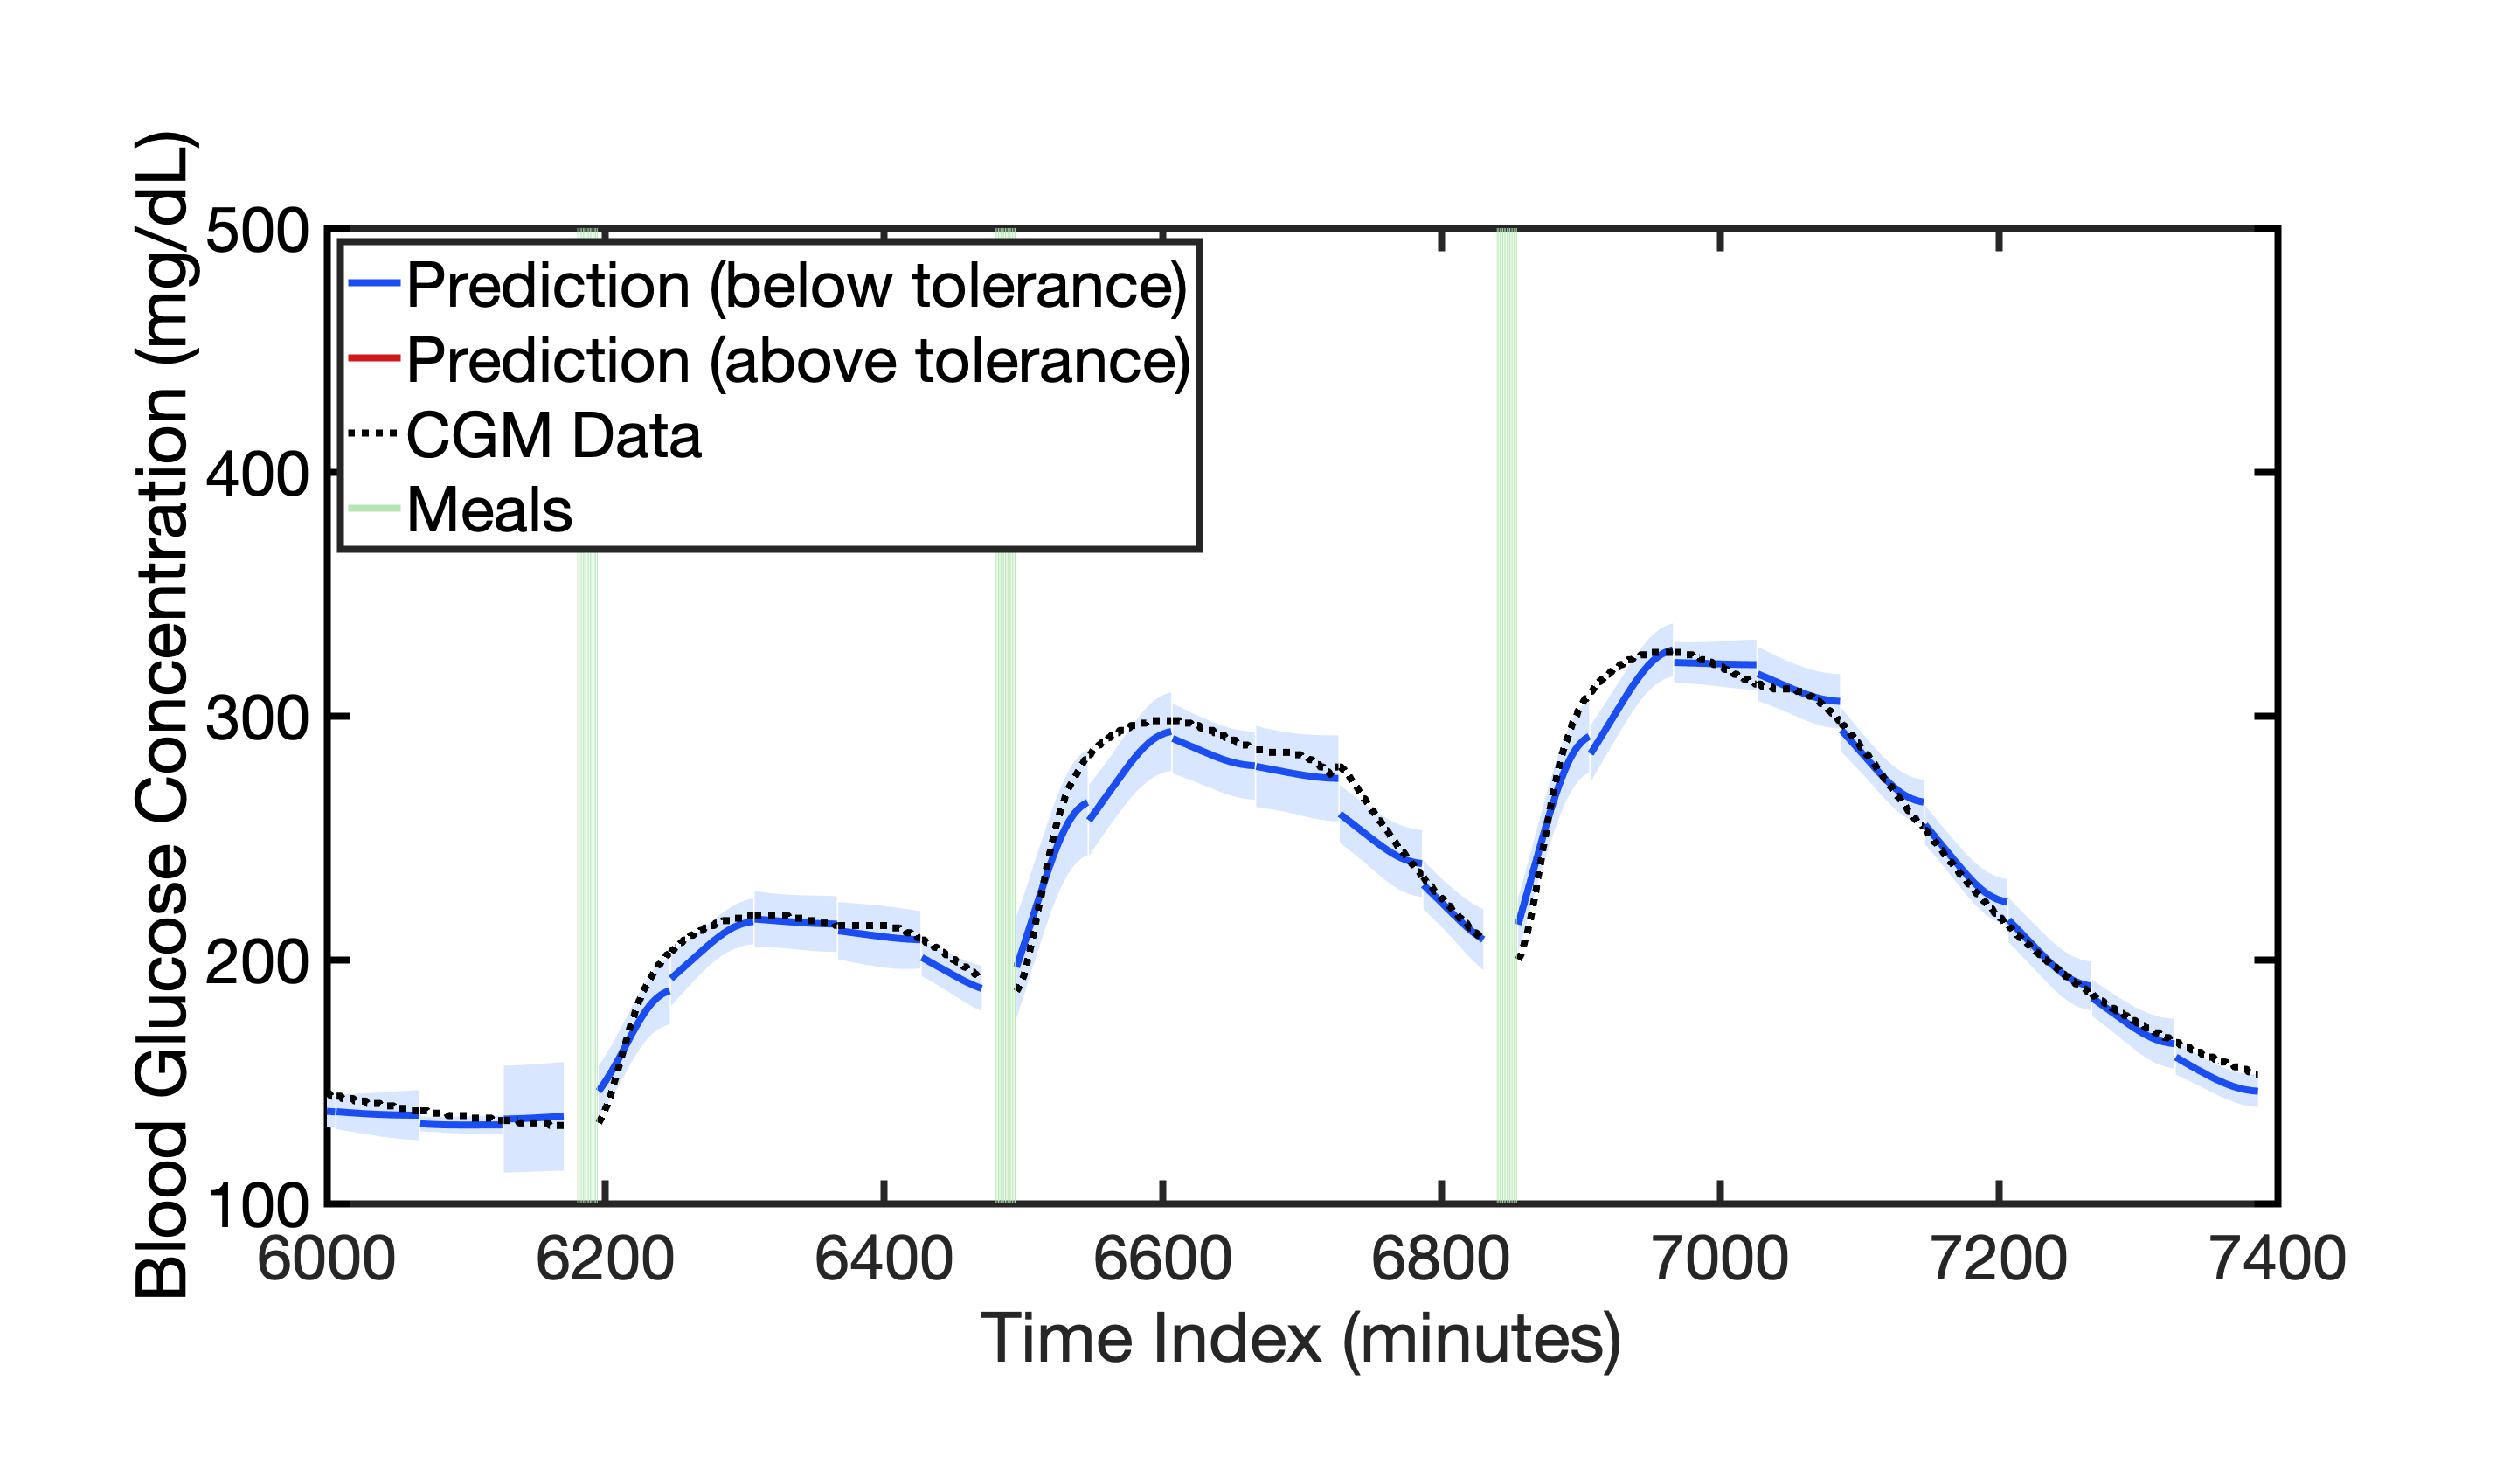
\includegraphics[width=\linewidth]{Figures/Part B/cat2/p1_c2.png}
  \caption*{(a)}
\end{minipage}\hfill
\begin{minipage}[t]{0.48\textwidth}
  \centering
  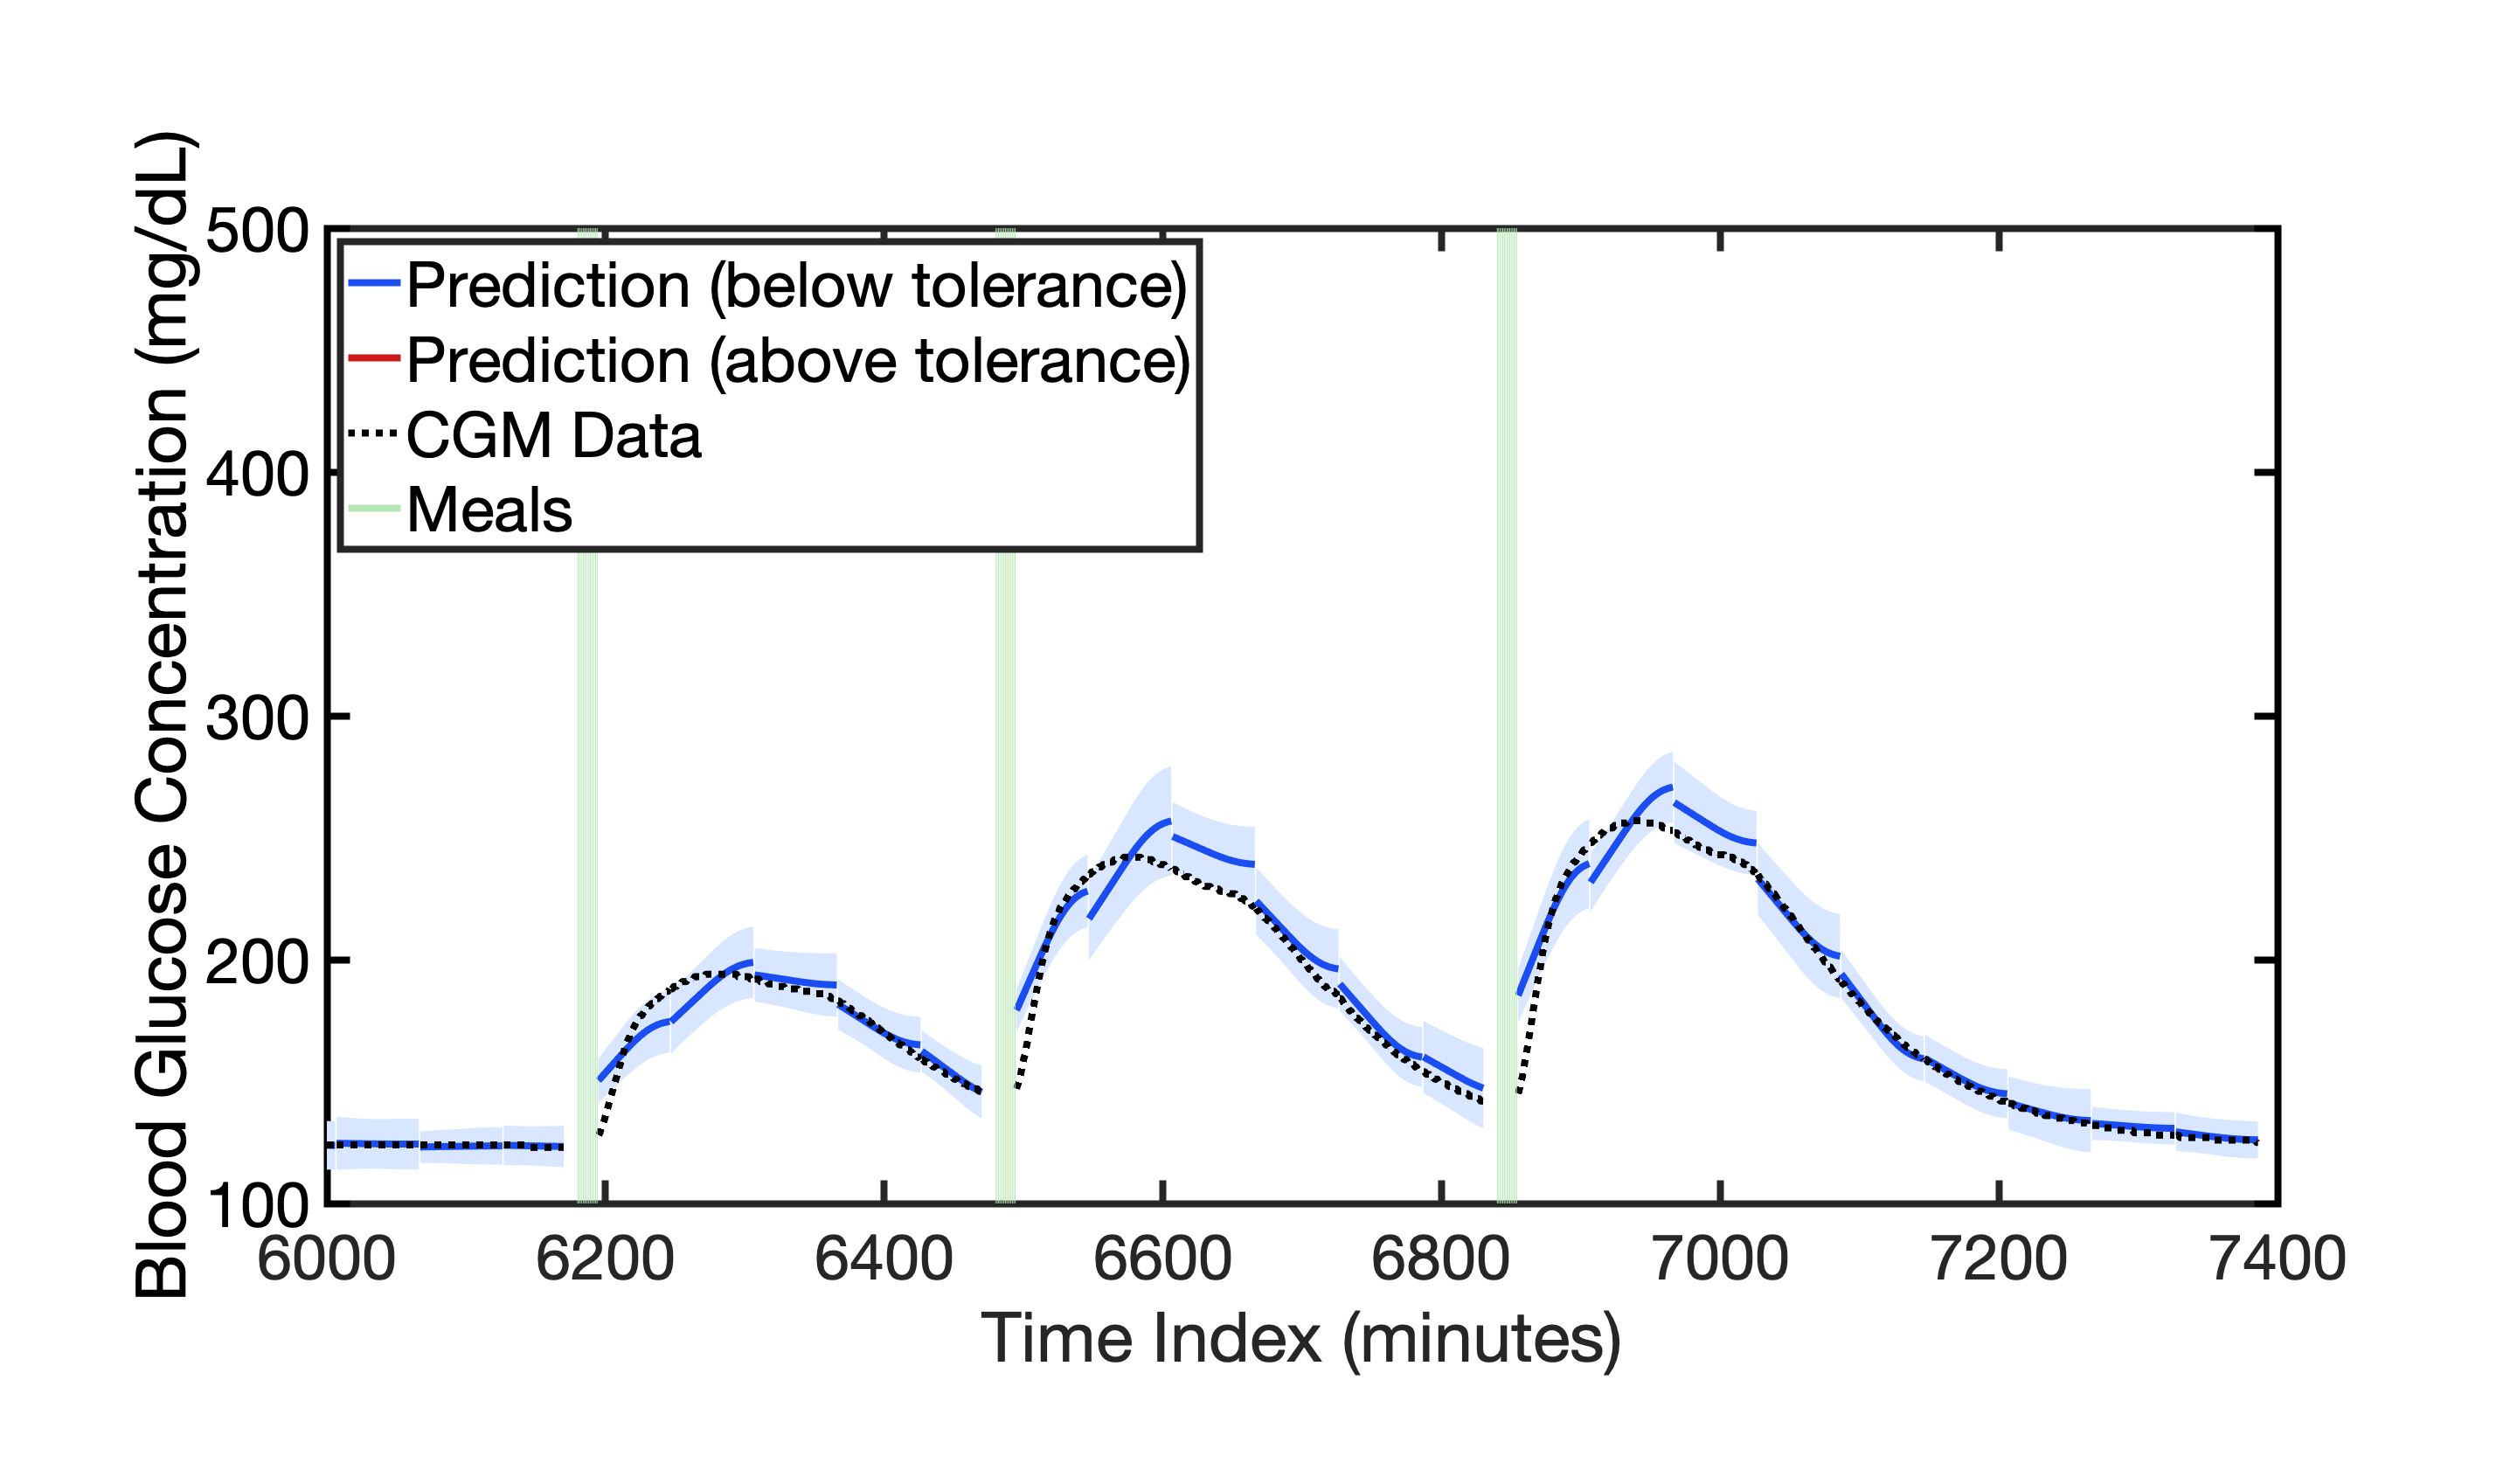
\includegraphics[width=\linewidth]{Figures/Part B/cat2/p2_c2.png}
  \caption*{(b)}
\end{minipage}

\begin{minipage}[t]{0.48\textwidth}
  \centering
  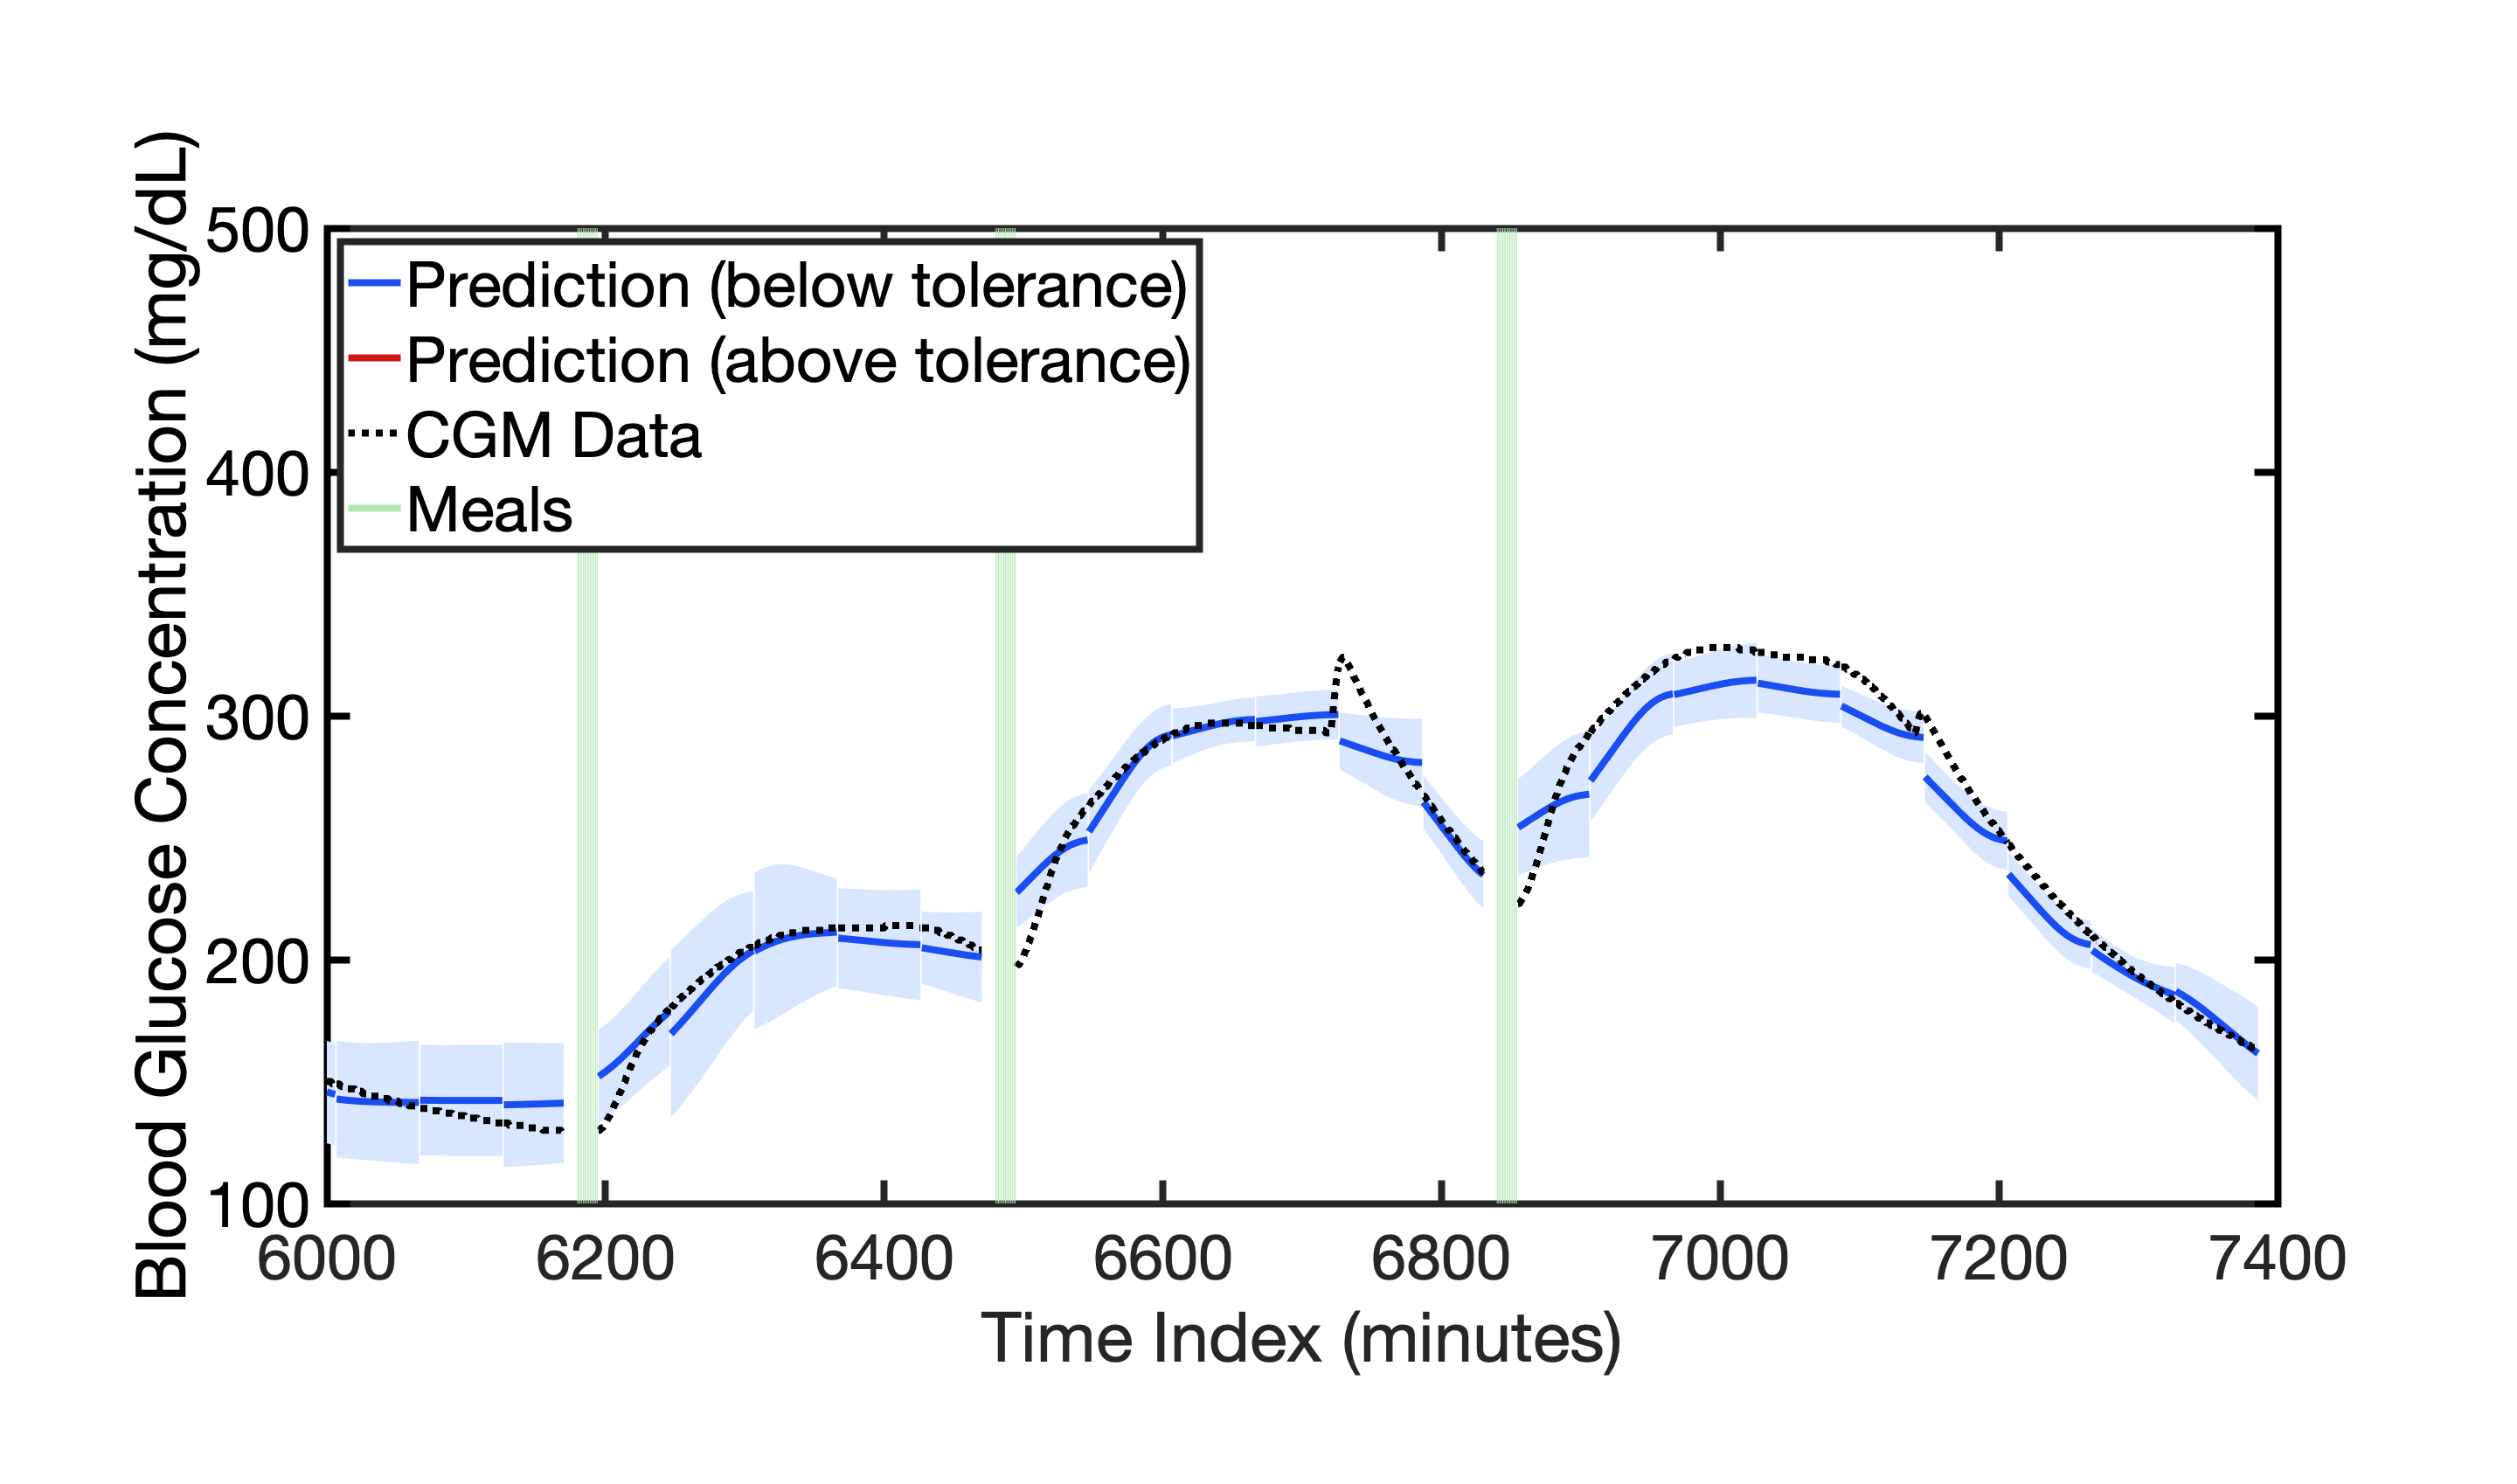
\includegraphics[width=\linewidth]{Figures/Part B/cat2/p3_c2.png}
  \caption*{(c)}
\end{minipage}\hfill
\begin{minipage}[t]{0.48\textwidth}
  \centering
  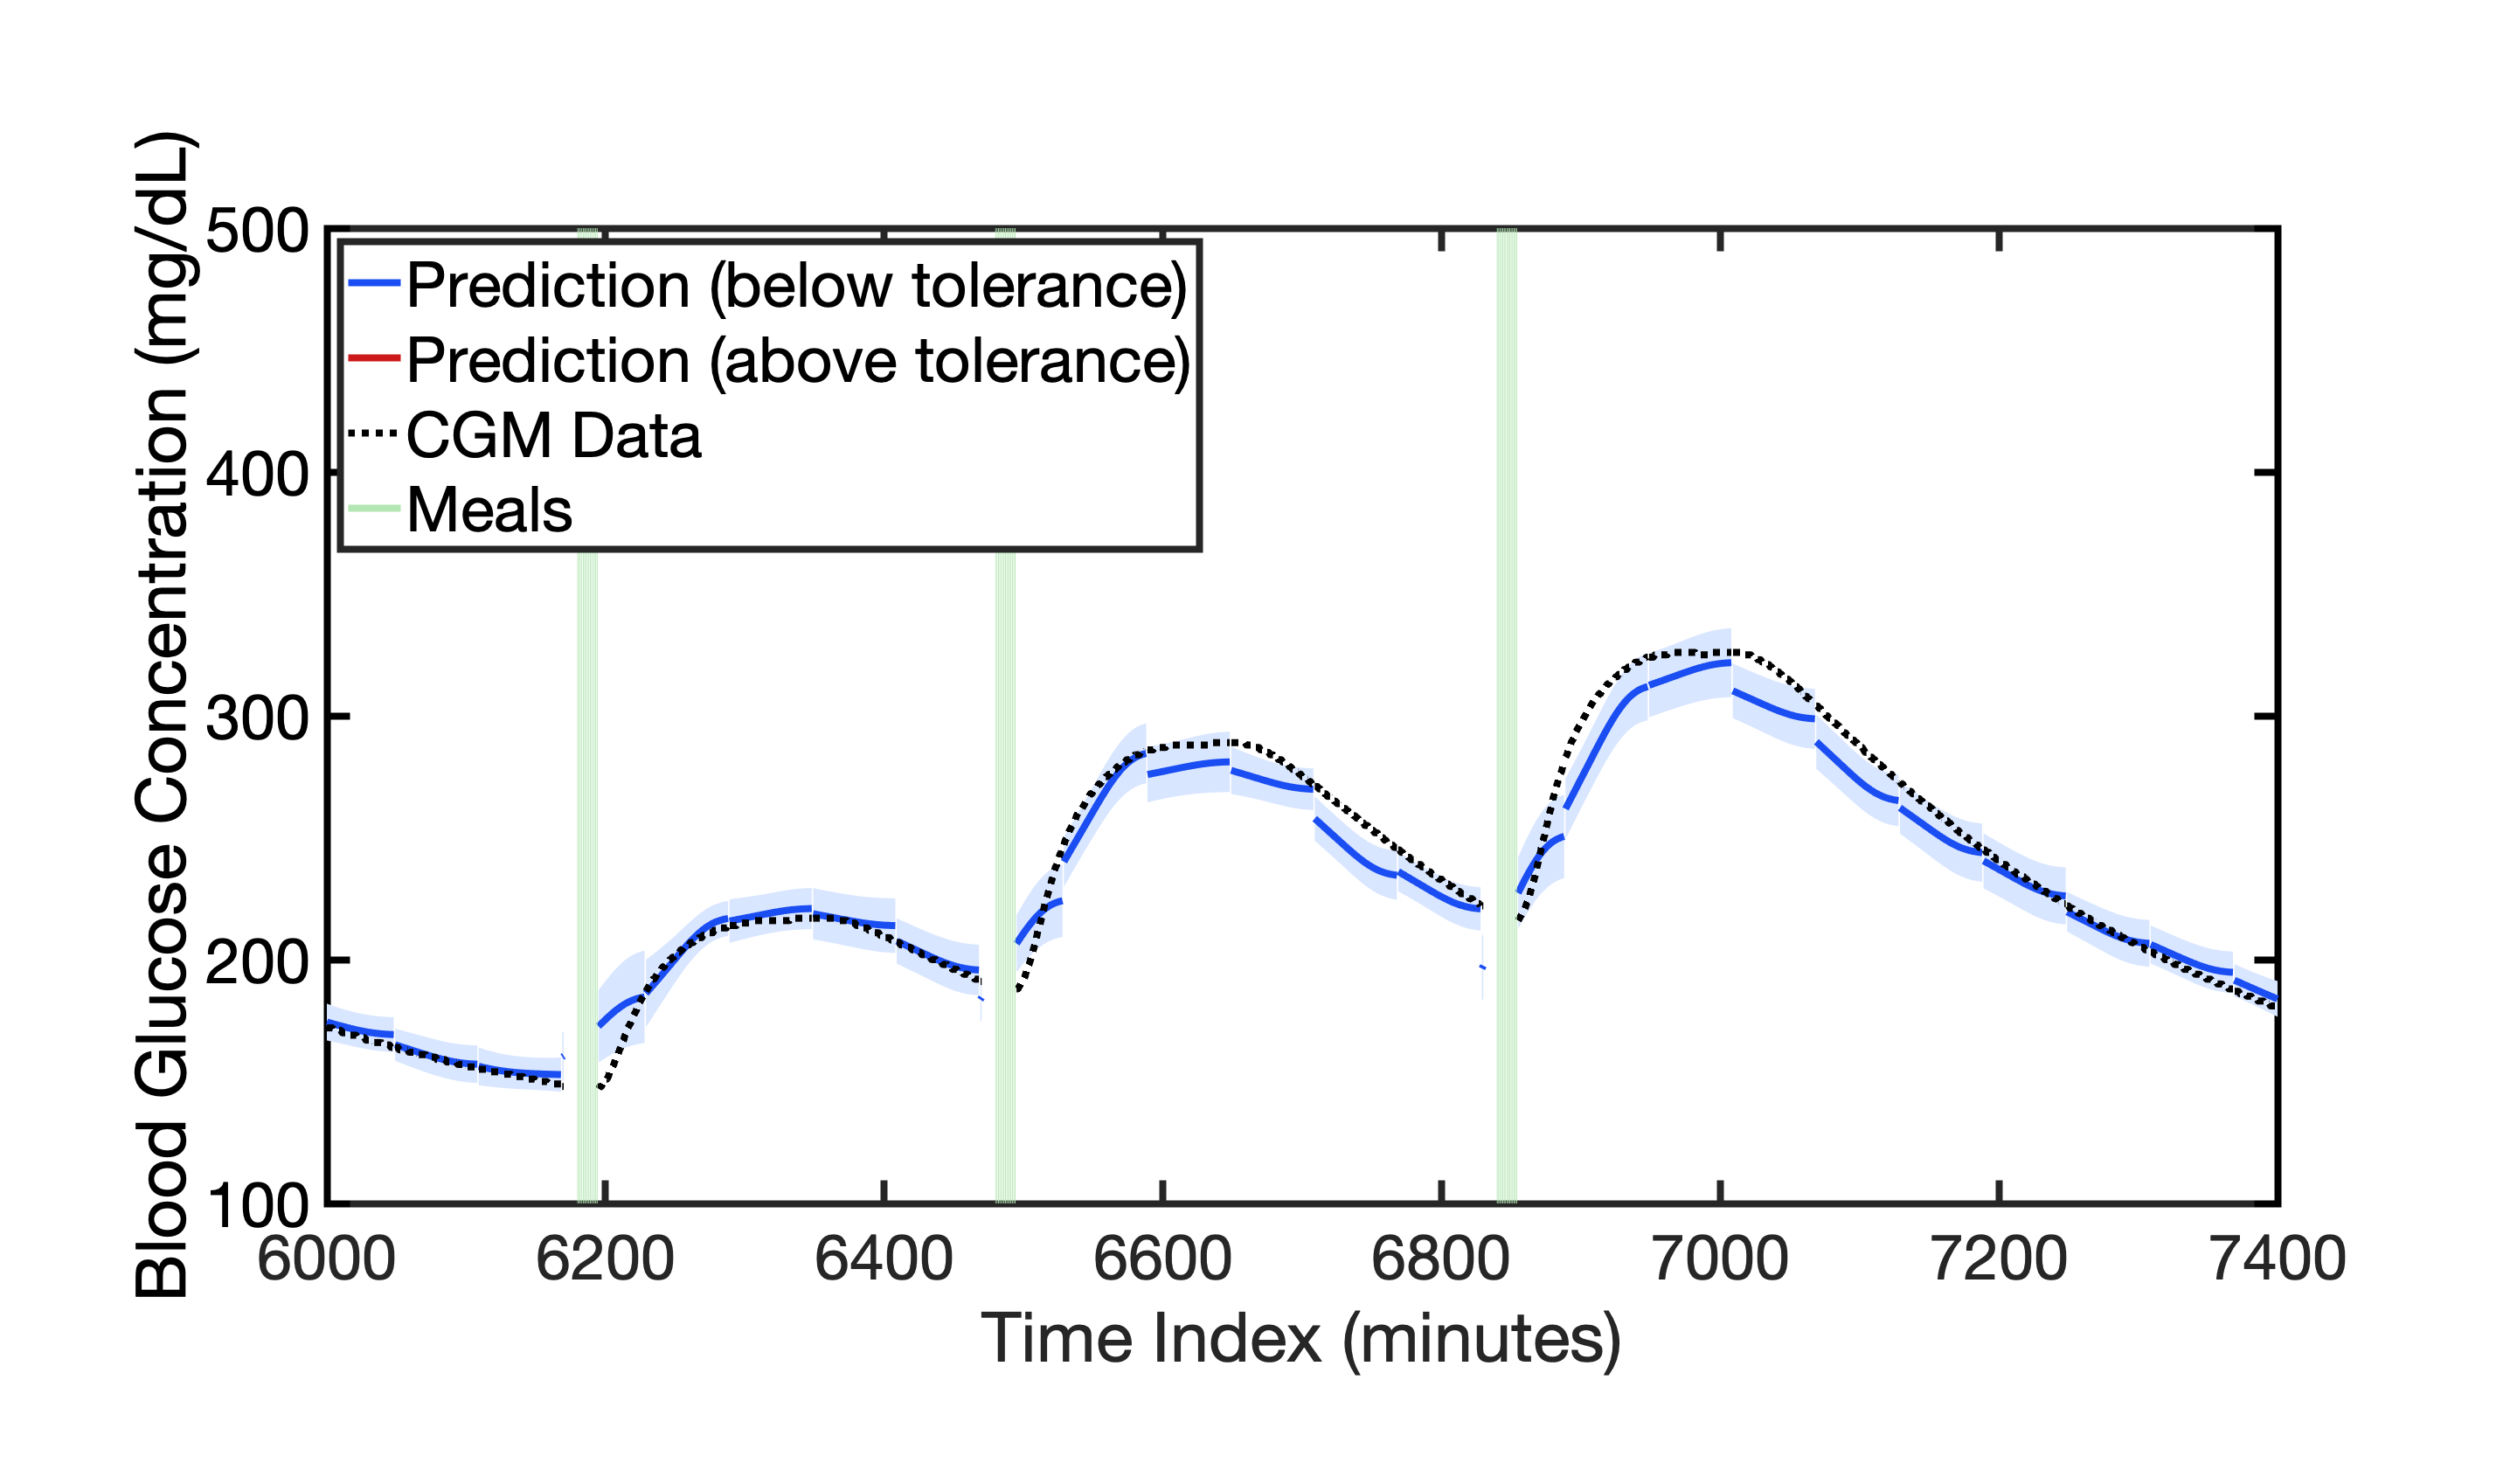
\includegraphics[width=\linewidth]{Figures/Part B/cat2/p4_c2.png}
  \caption*{(d)}
\end{minipage}

\caption{(a) Patient 1 from fold 3, Architecture: $Cat_2Arch_4$, (b) Patient 2 from fold 3, Architecture: $Cat_2Arch_4$, (c) Patient 3 from fold 4, Architecture: $Cat_2Arch_4$, and (d) Patient 4 from fold 4,, Architecture: $Cat_2Arch_4$.}
\label{fig:cat2_success}
\end{figure}



Comparison of success architecture with model averaging: in Category 2 compare for both leave-out patients predictions of individual architectures with the Bayesian model averaging prediction. Do this for two folds (#2) where model plausibility values vary more significantly across the 10 architectures  (arrange 2x2)=> Maybe show NLPD plots for each segment?

While Category~2 produces DT-usable models in most folds, we observed that a single plausible architecture can still fail the validation criterion in specific leave-out regimes. To analize te effect of each architecture and their corresponding plausibility, we apply Bayesian model averaging (BMA) over all of the architectures and evaluate the resulting predictive distribution on the same validation windows. Fold~2 in \autoref{fig:bma} provides a representative example of how Bayesian model averaging (BMA) can enhance predictive performance, particularly in folds where multiple architectures exhibit comparable posterior plausibility.

Let $\mathcal{M}_1,\ldots,\mathcal{M}_K$ denote the $K$ candidate architectures in a fold and $\rho_m$ be their normalized posterior model plausibility. Each model provides a Gaussian predictive distribution at time index $t$,
$p(G_t \mid \mathcal{M}_k, \mathcal{D}) = \mathcal{N}\!\big(\mu_{k,t},\,\sigma_{k,t}^2\big)$,
so the BMA predictive distribution is a Gaussian mixture:
\begin{equation}
p(G_t \mid \mathcal{D})
\;=\;
\sum_{k=1}^K \rho_m \, \mathcal{N}\!\big(\mu_{k,t},\sigma_{k,t}^2\big).
\label{eq:bma_mixture}
\end{equation}

BMA improves prediction in two ways: (i) the averaged mean $\mu^{\text{BMA}}_t$ is less sensitive to a single model's transient bias and incorporates weighted mean from all architectures, and (ii) the predictive uncertainty increases in precisely the regions where the ensemble disagrees, preventing overly sharp likelihood penalties. Using a small plausibility-weighted ensemble is more accurate than committing to one architecture per fold. 


\begin{figure}[H]
\centering

\begin{minipage}[t]{0.48\textwidth}
  \centering
  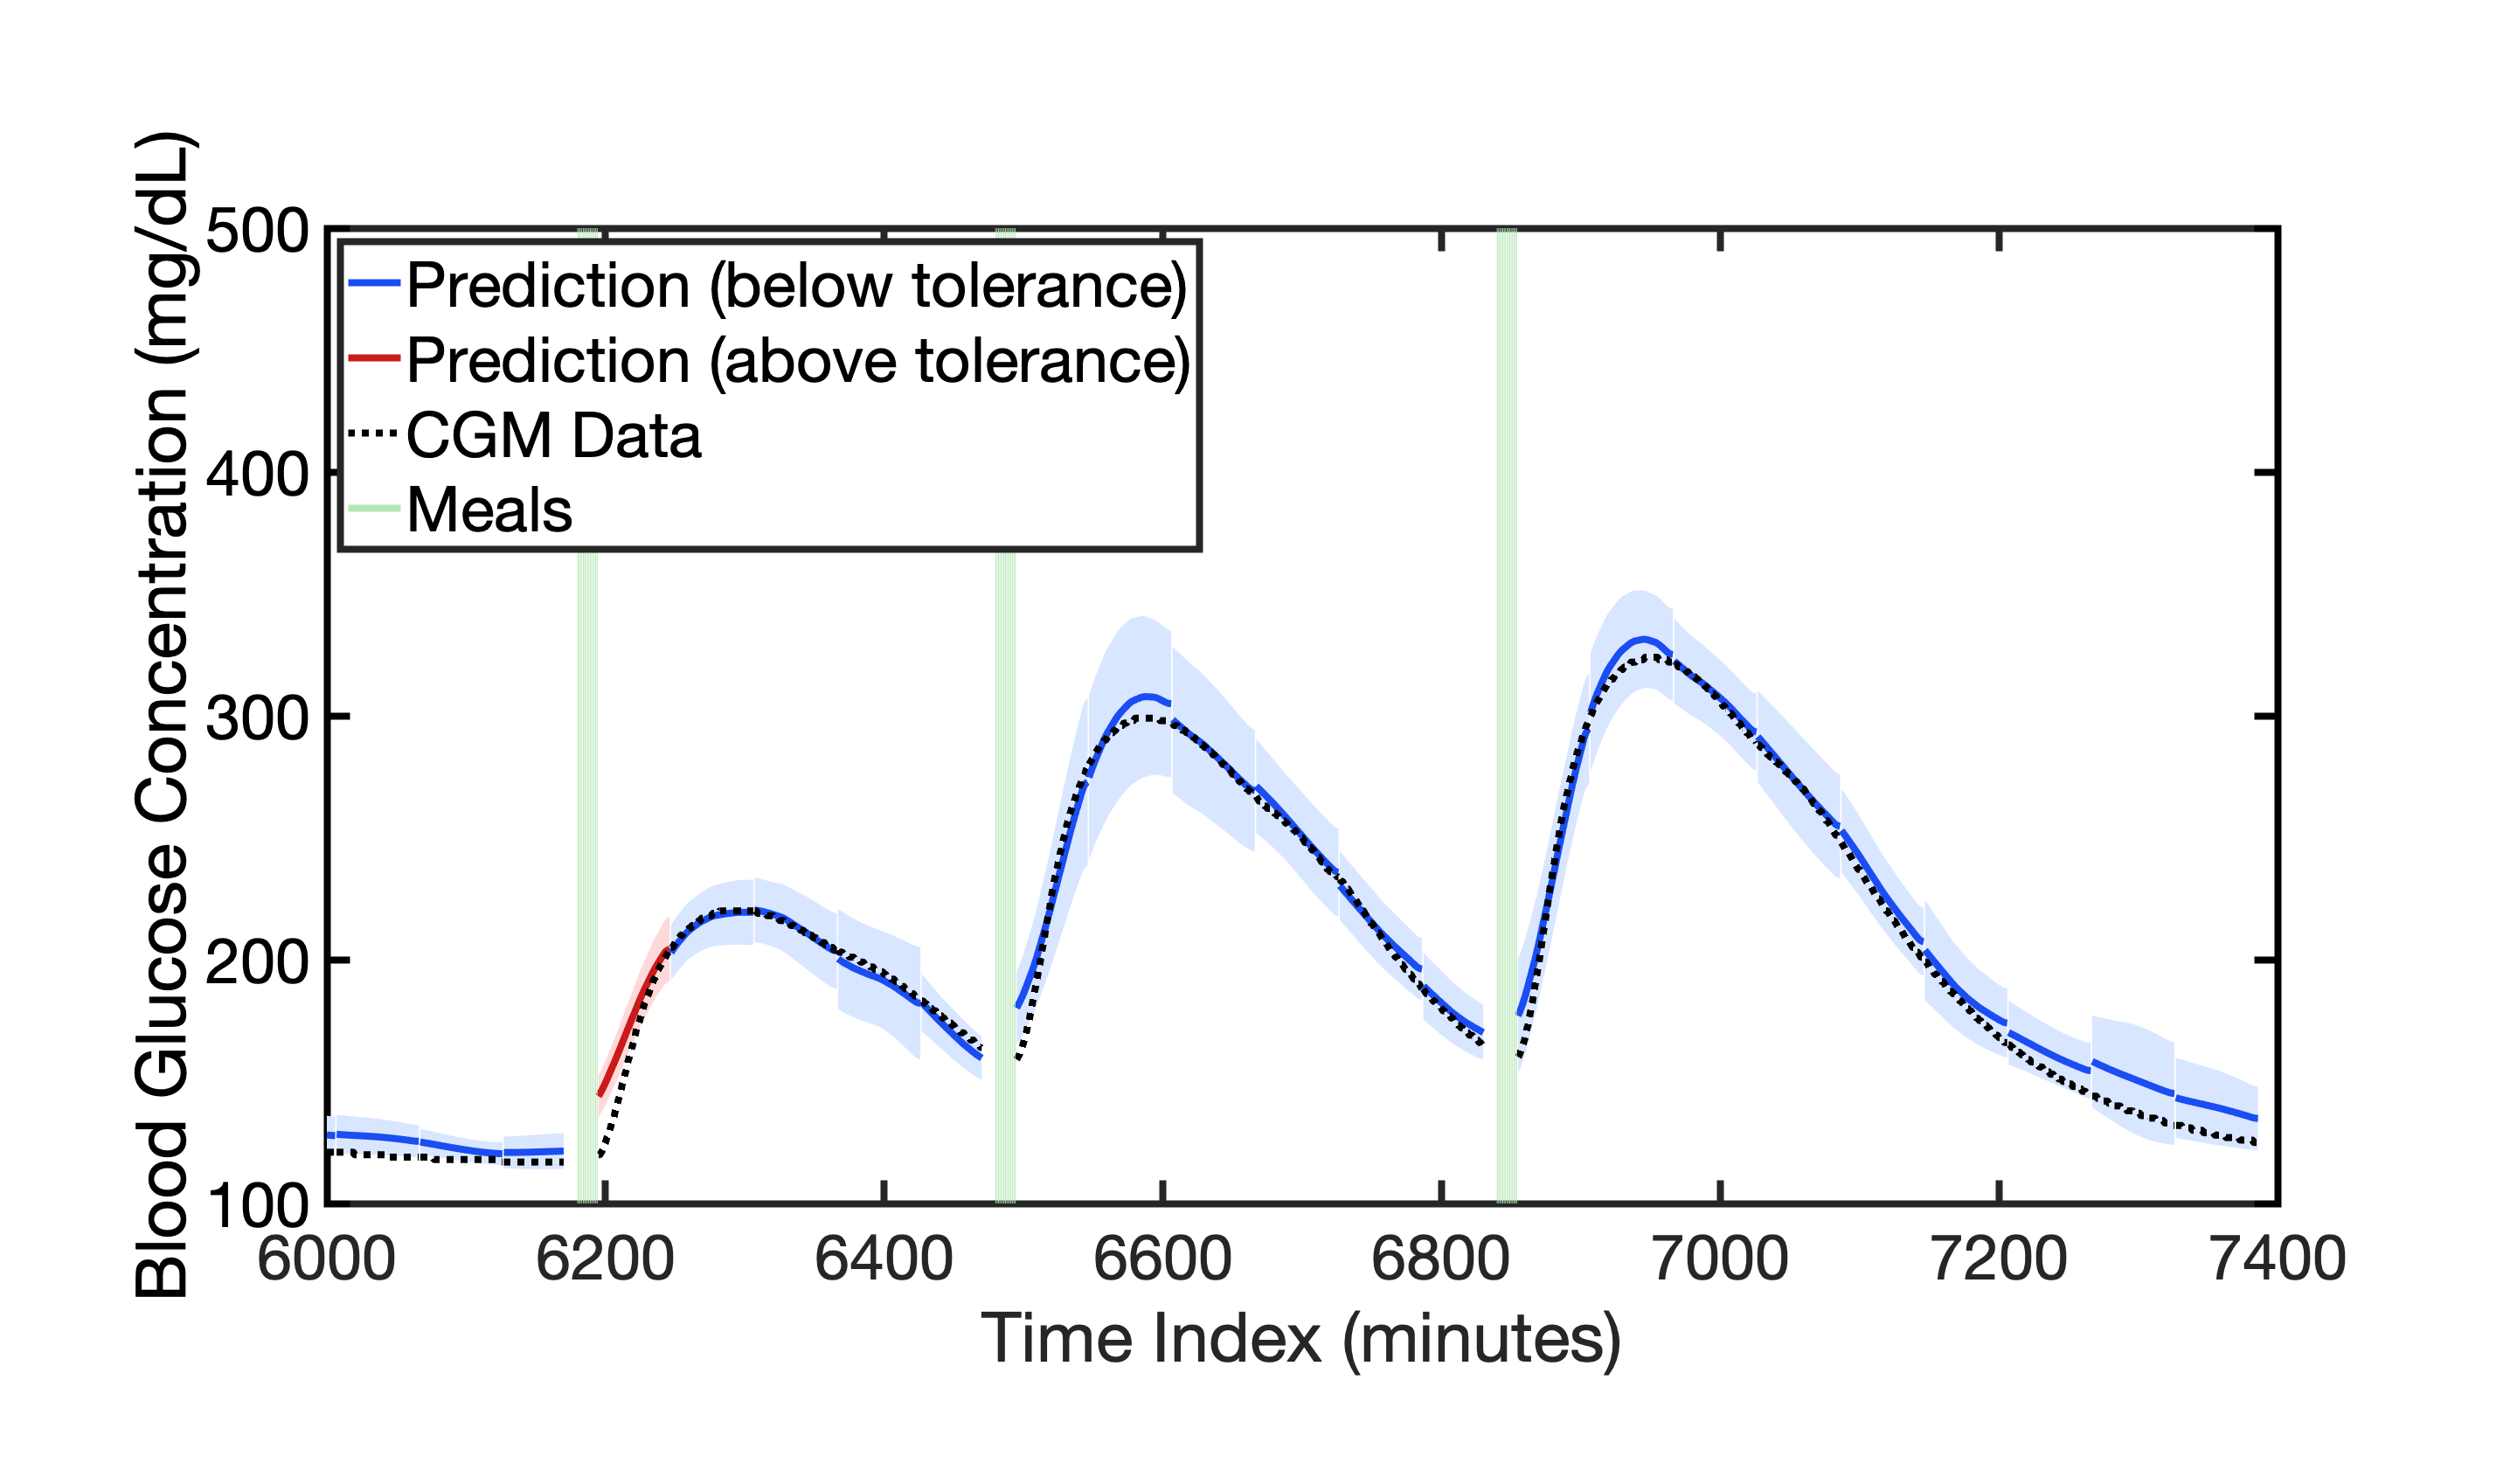
\includegraphics[width=\linewidth]{Figures/Part B/cat2/p6_c2.png}
  \caption*{(a)}
\end{minipage}\hfill
\begin{minipage}[t]{0.48\textwidth}
  \centering
  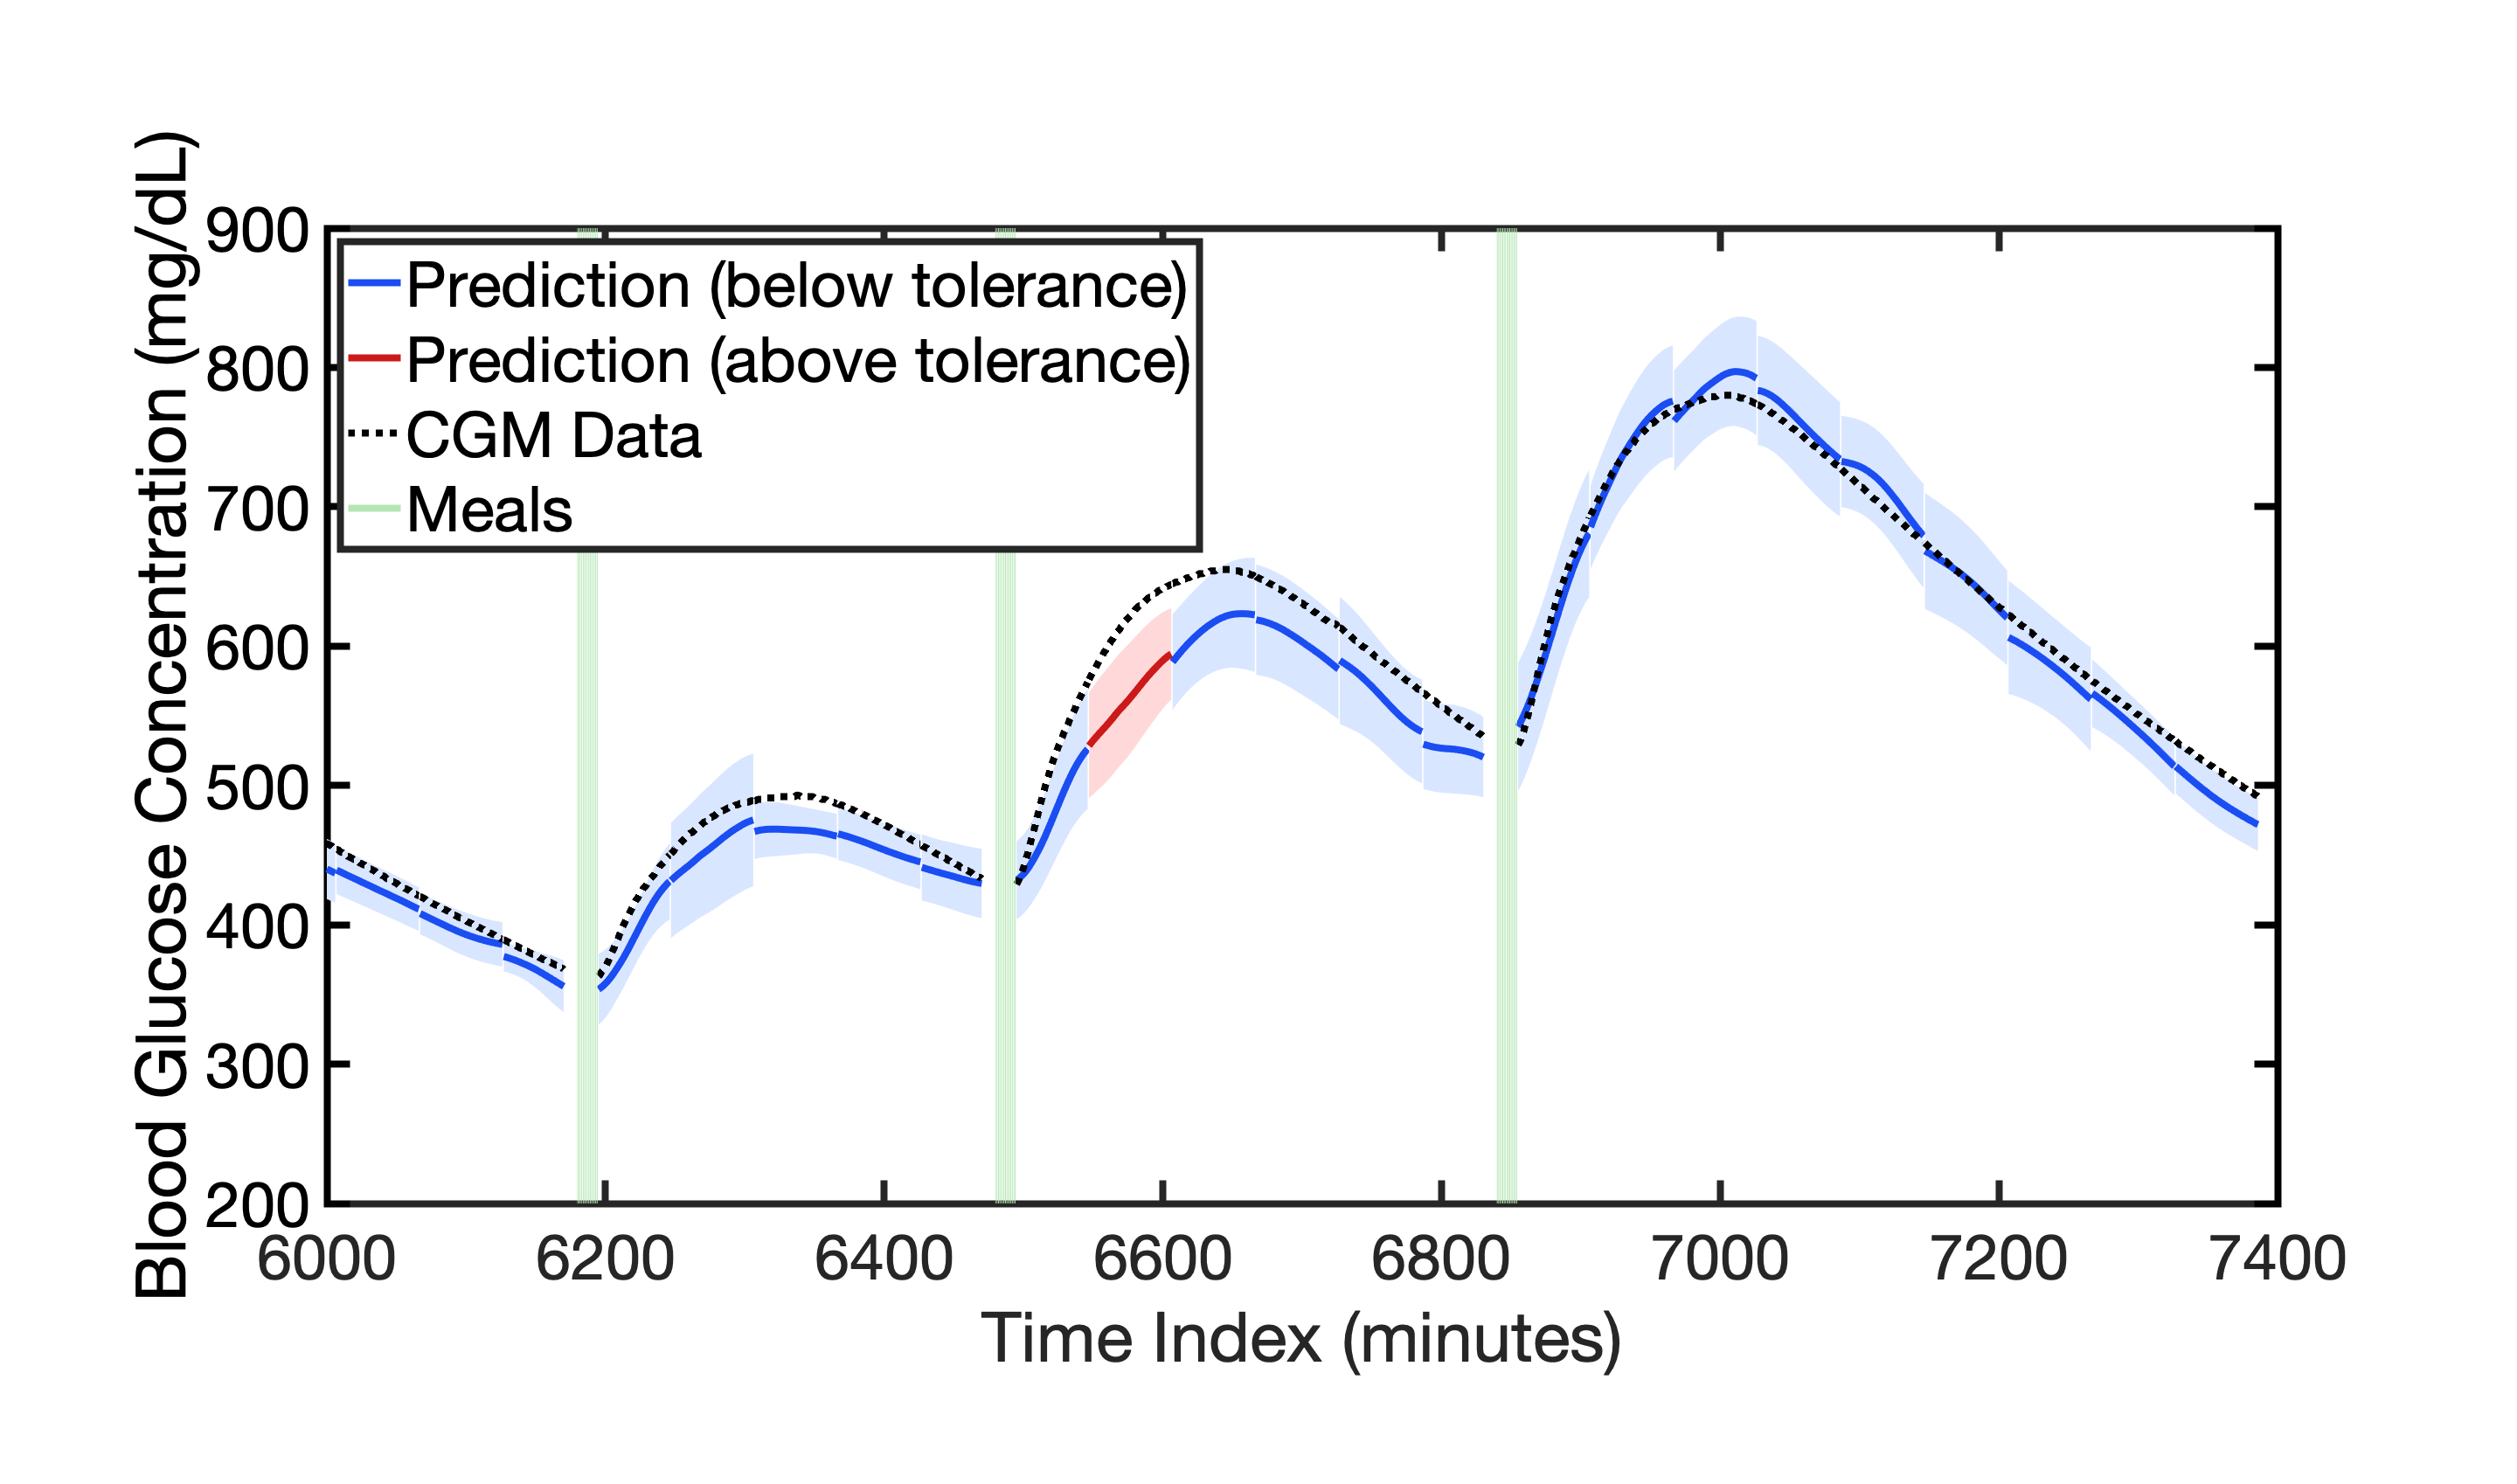
\includegraphics[width=\linewidth]{Figures/Part B/cat2/p7_c2.png}
  \caption*{(b)}
\end{minipage}

\begin{minipage}[t]{0.48\textwidth}
  \centering
  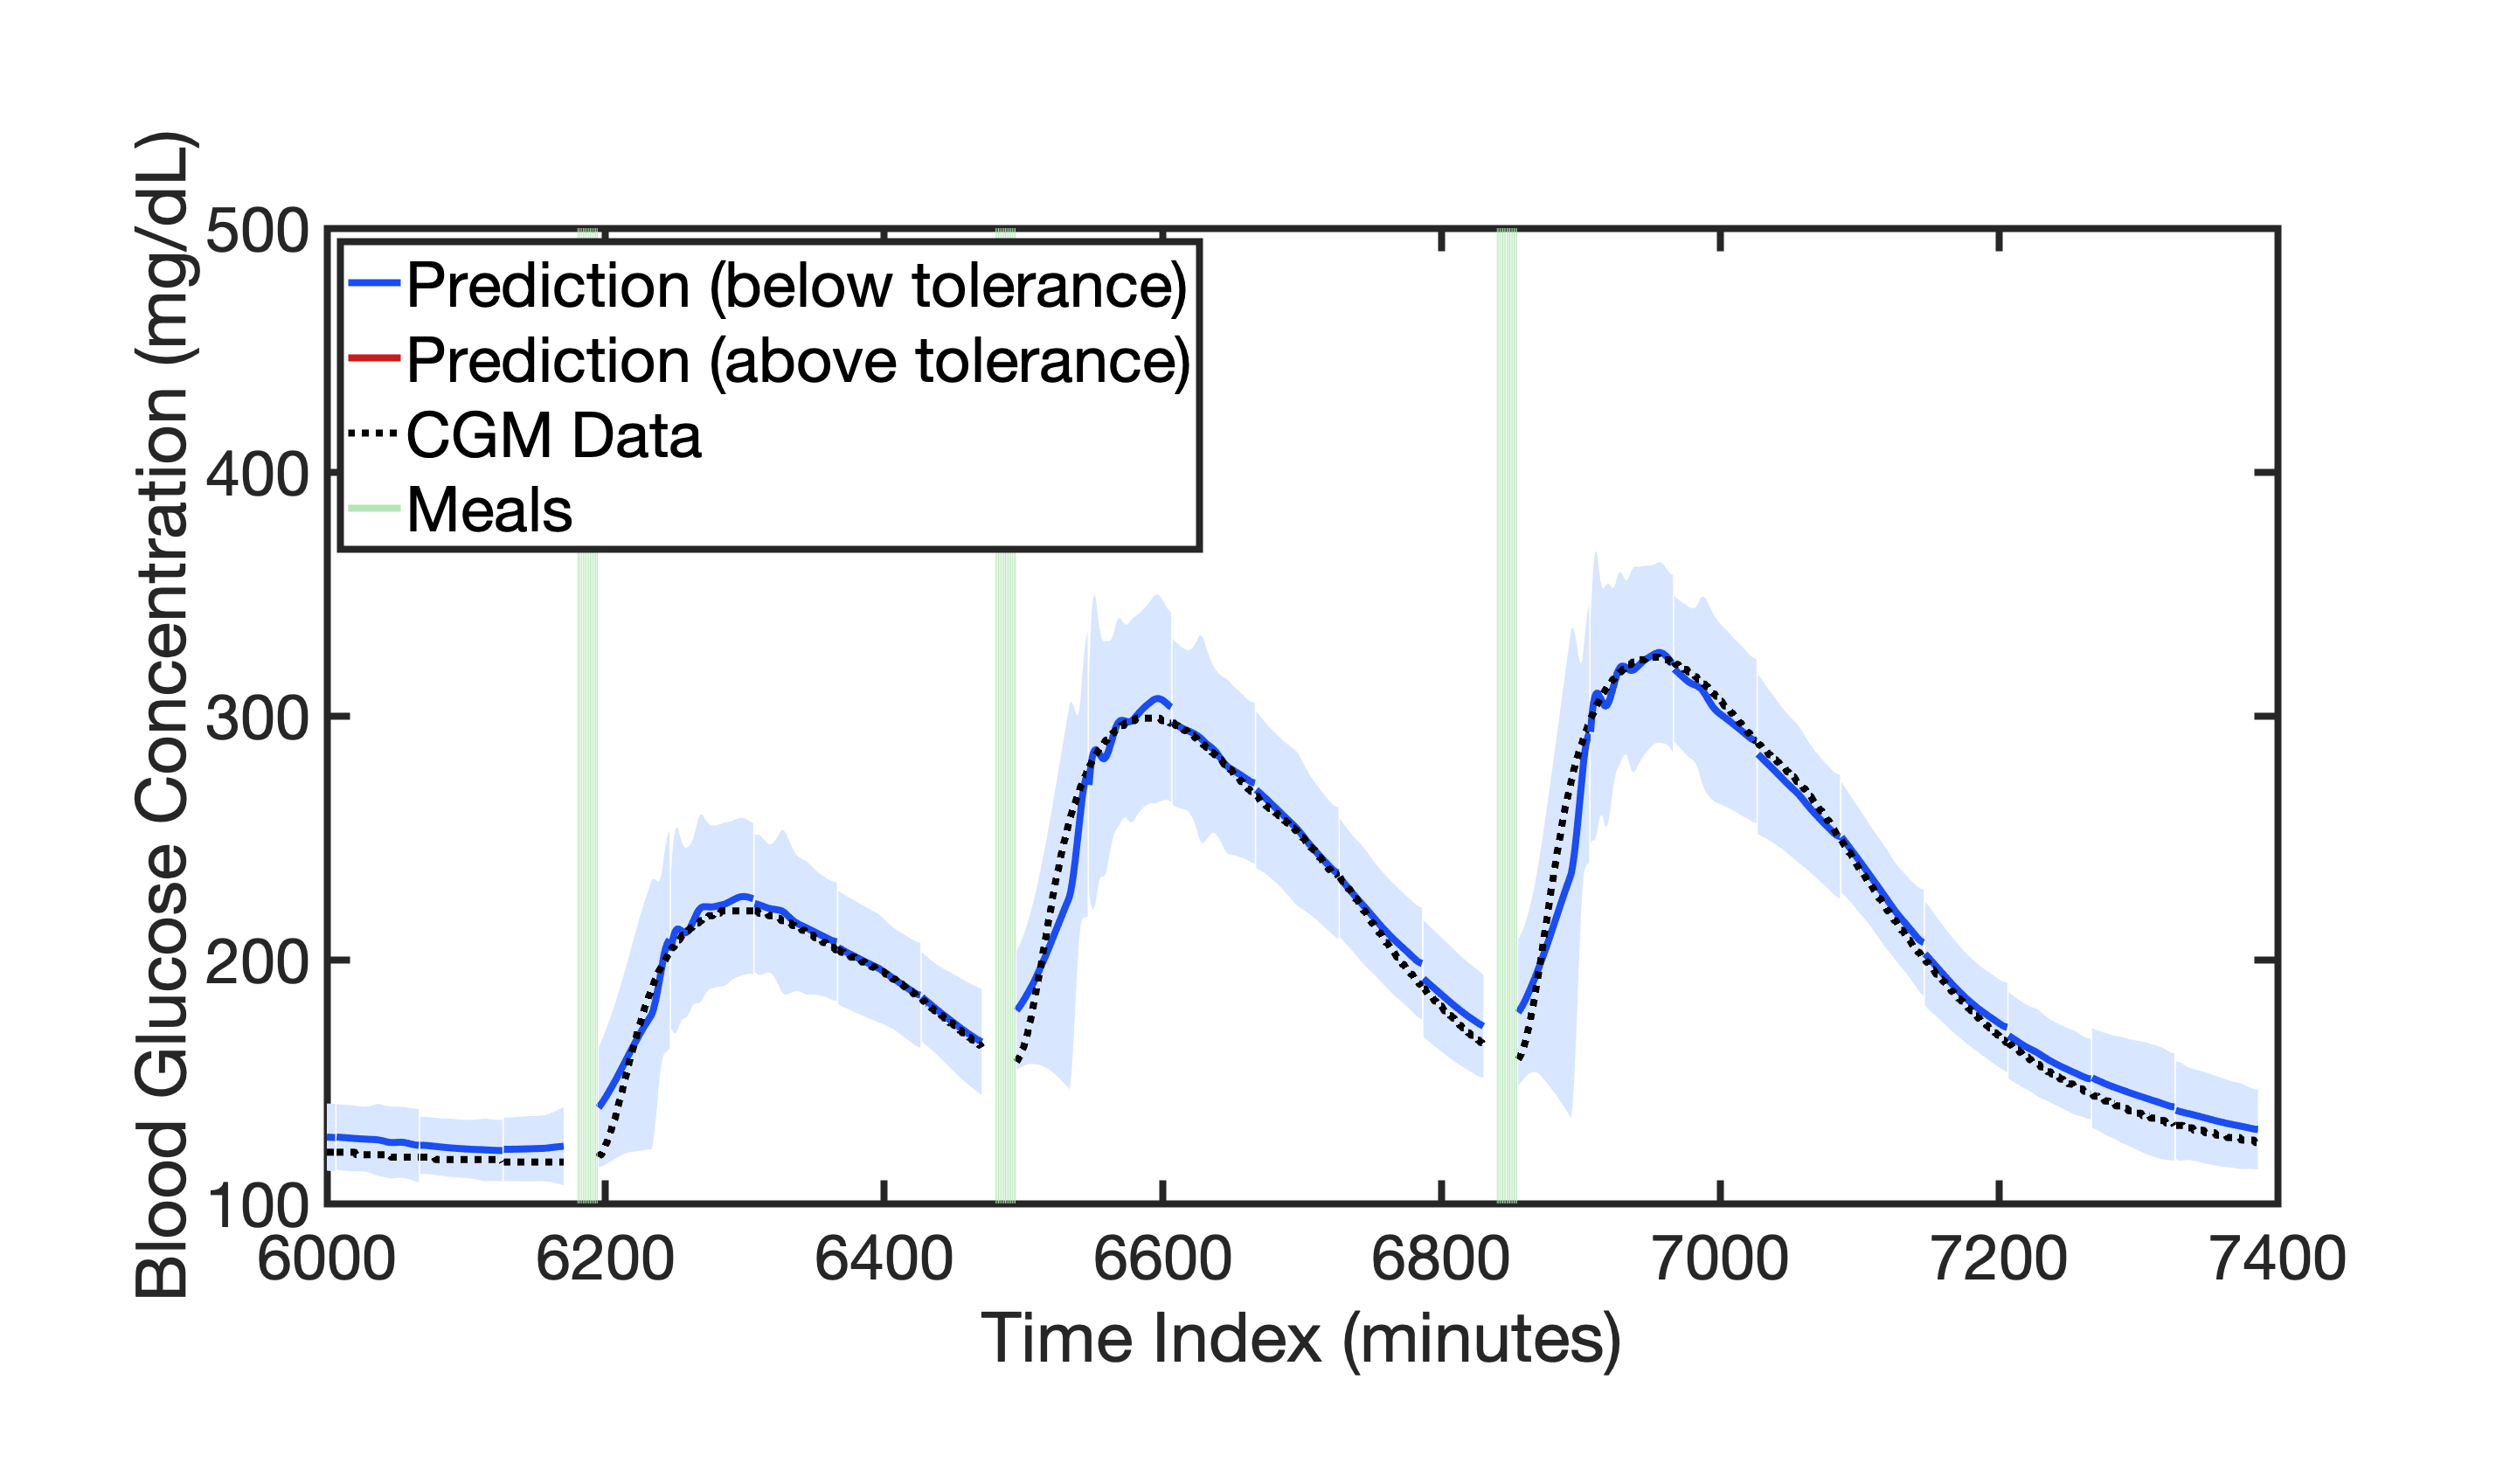
\includegraphics[width=\linewidth]{Figures/Part B/cat2/p6_bma.png}
  \caption*{(c)}
\end{minipage}\hfill
\begin{minipage}[t]{0.48\textwidth}
  \centering
  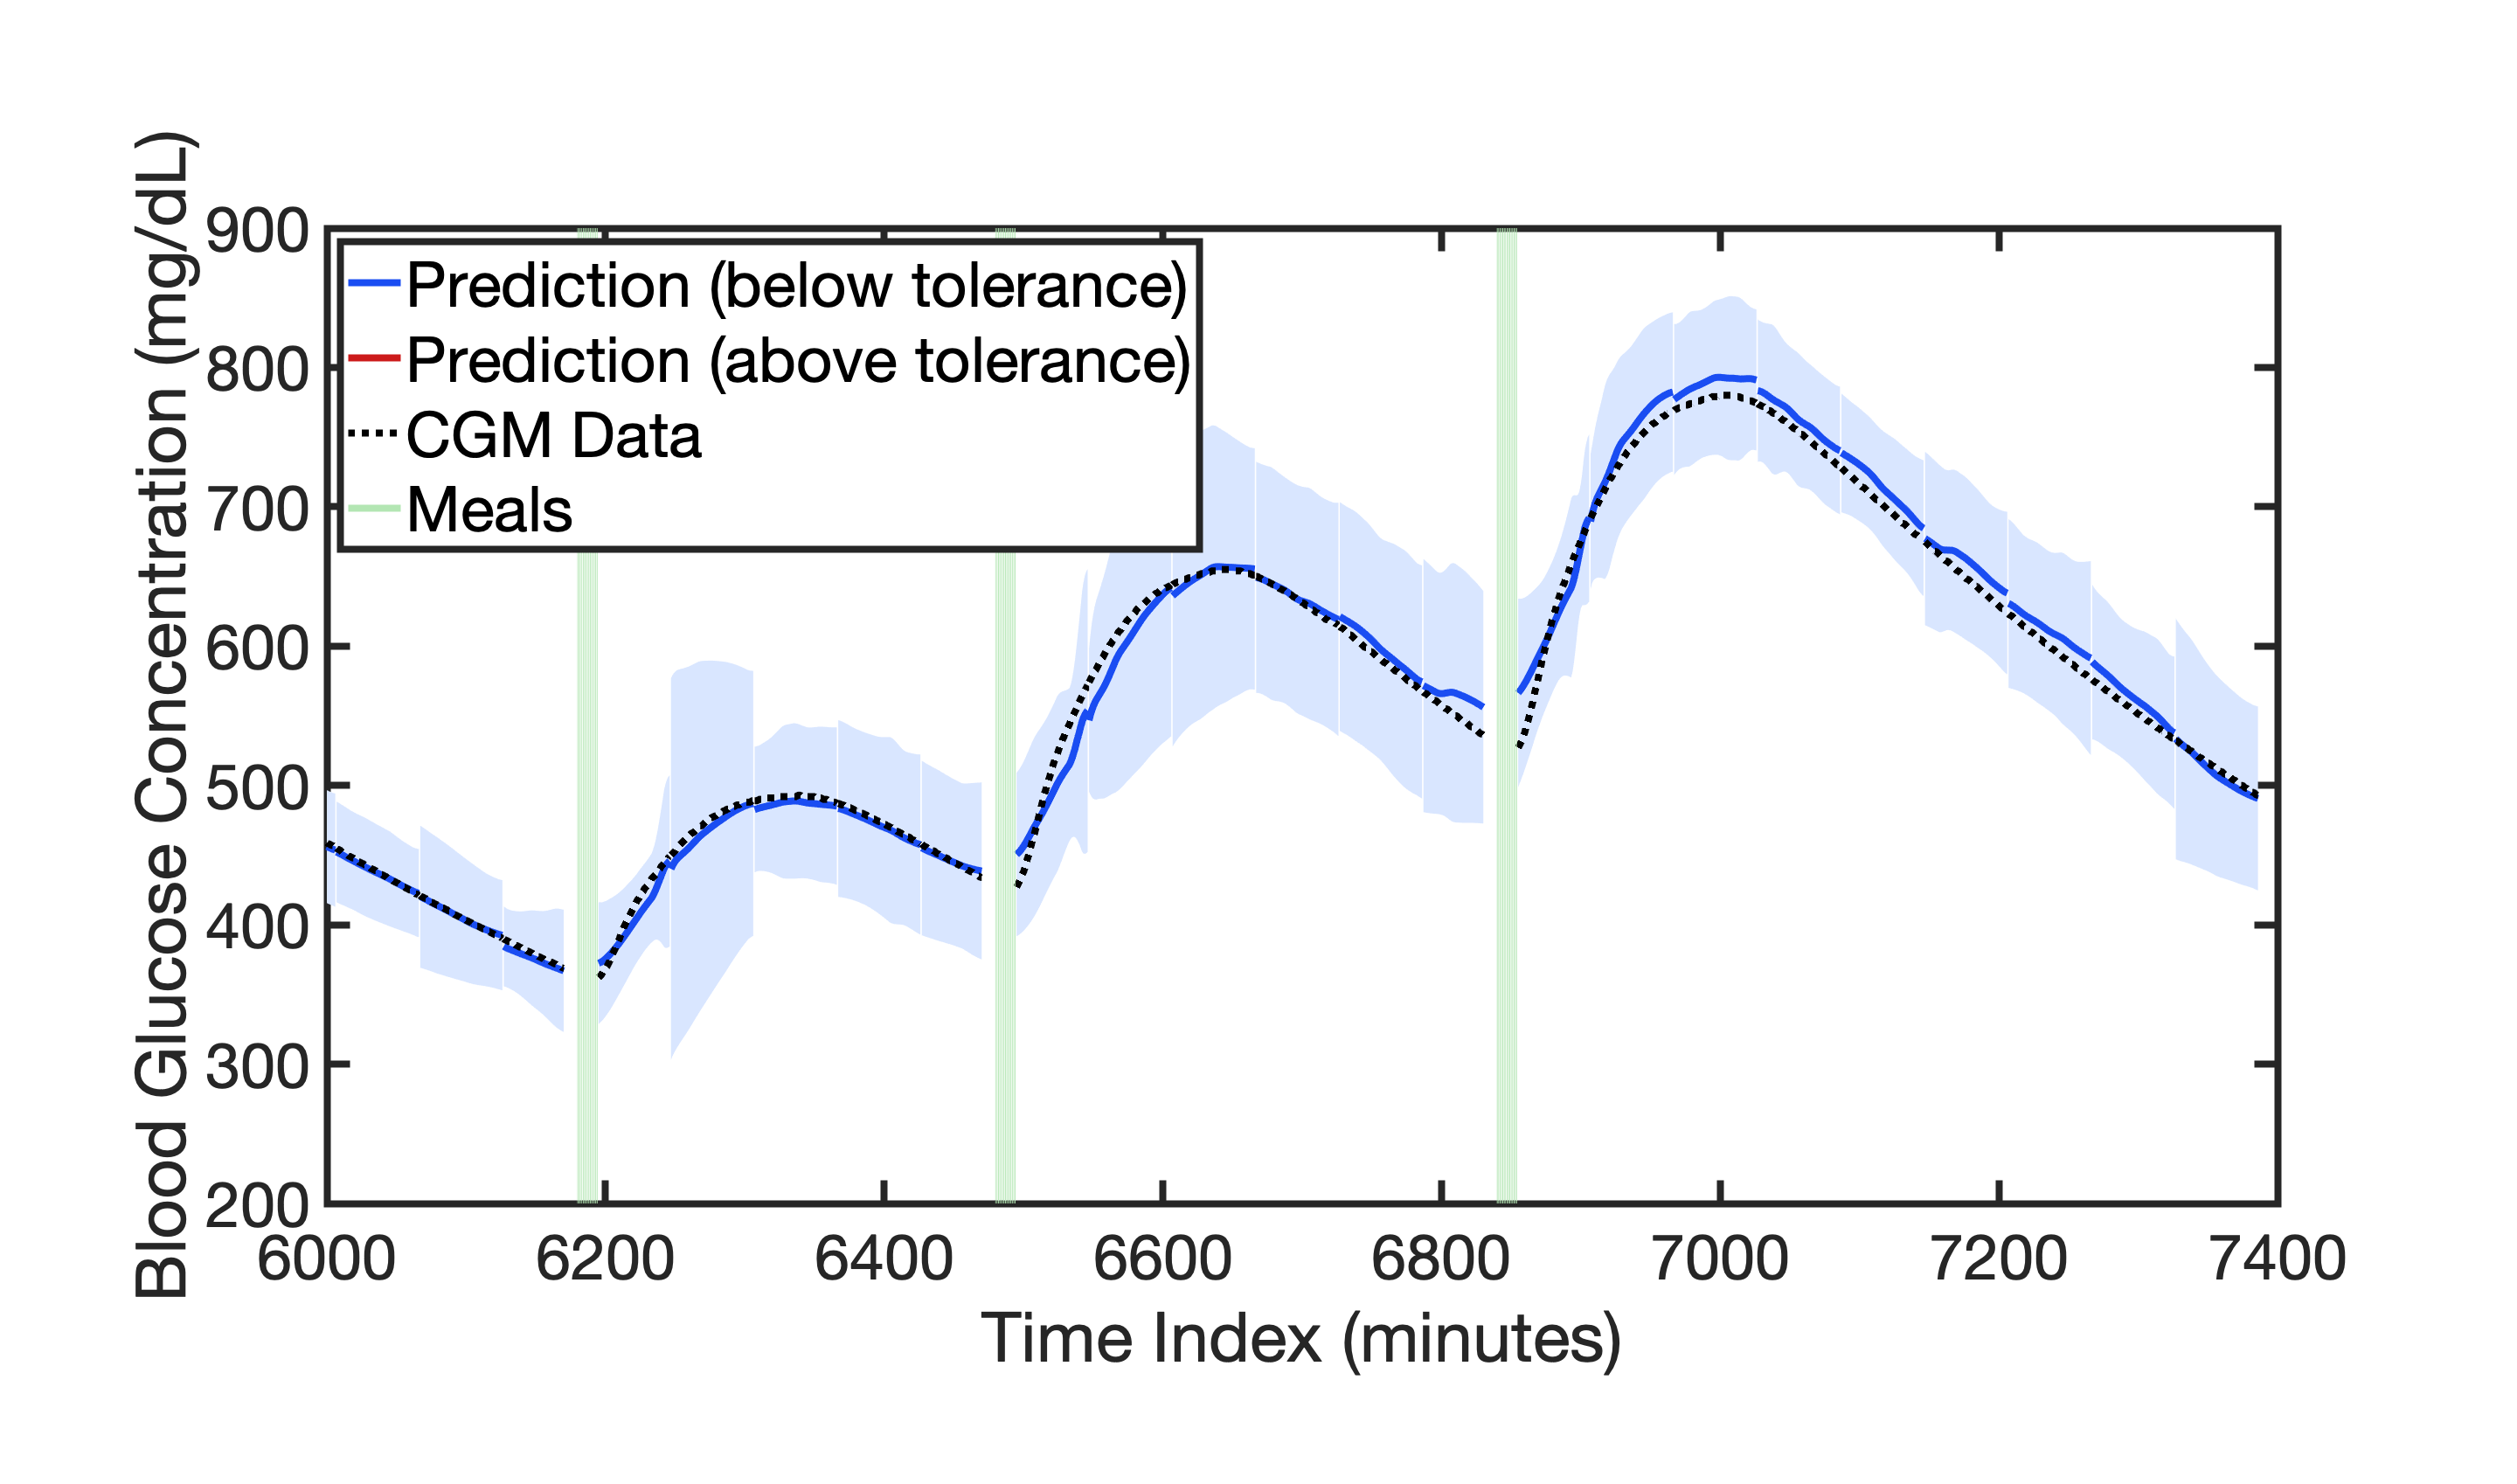
\includegraphics[width=\linewidth]{Figures/Part B/cat2/p7_bma.png}
  \caption*{(d)}
\end{minipage}

\caption{(a) Patient 6 from fold 2, Architecture: $Cat_2Arch_7$, (b) Patient 7 from fold 2, Architecture: $Cat_2Arch_7$, (c) Patient 6 from fold 2 with Bayesian model averaging, and (d) Patient 7 from fold 2 with Bayesian model averaging}
\label{fig:bma}
\end{figure}



     \item Category 3: 4 (or even 2) validation data-model plots => conclude more complex category fails


Category 3 contains substantially complicated B-TCN candidates (approximately 100k–400k trainable parameters), created by increasing depth and/or channel widths relative to Category 2 while still satisfying the receptive-field feasibility constraints. In terms of concrete designs, the most plausible models in this bin typically include wider and deeper encoder–decoder stacks (via dilation/base and kernel-size choices), which increases representational capacity but also increases the number of weakly-informed parameter counts under the available training data.



\begin{figure}[H]
\centering

\begin{minipage}[t]{0.48\textwidth}
  \centering
  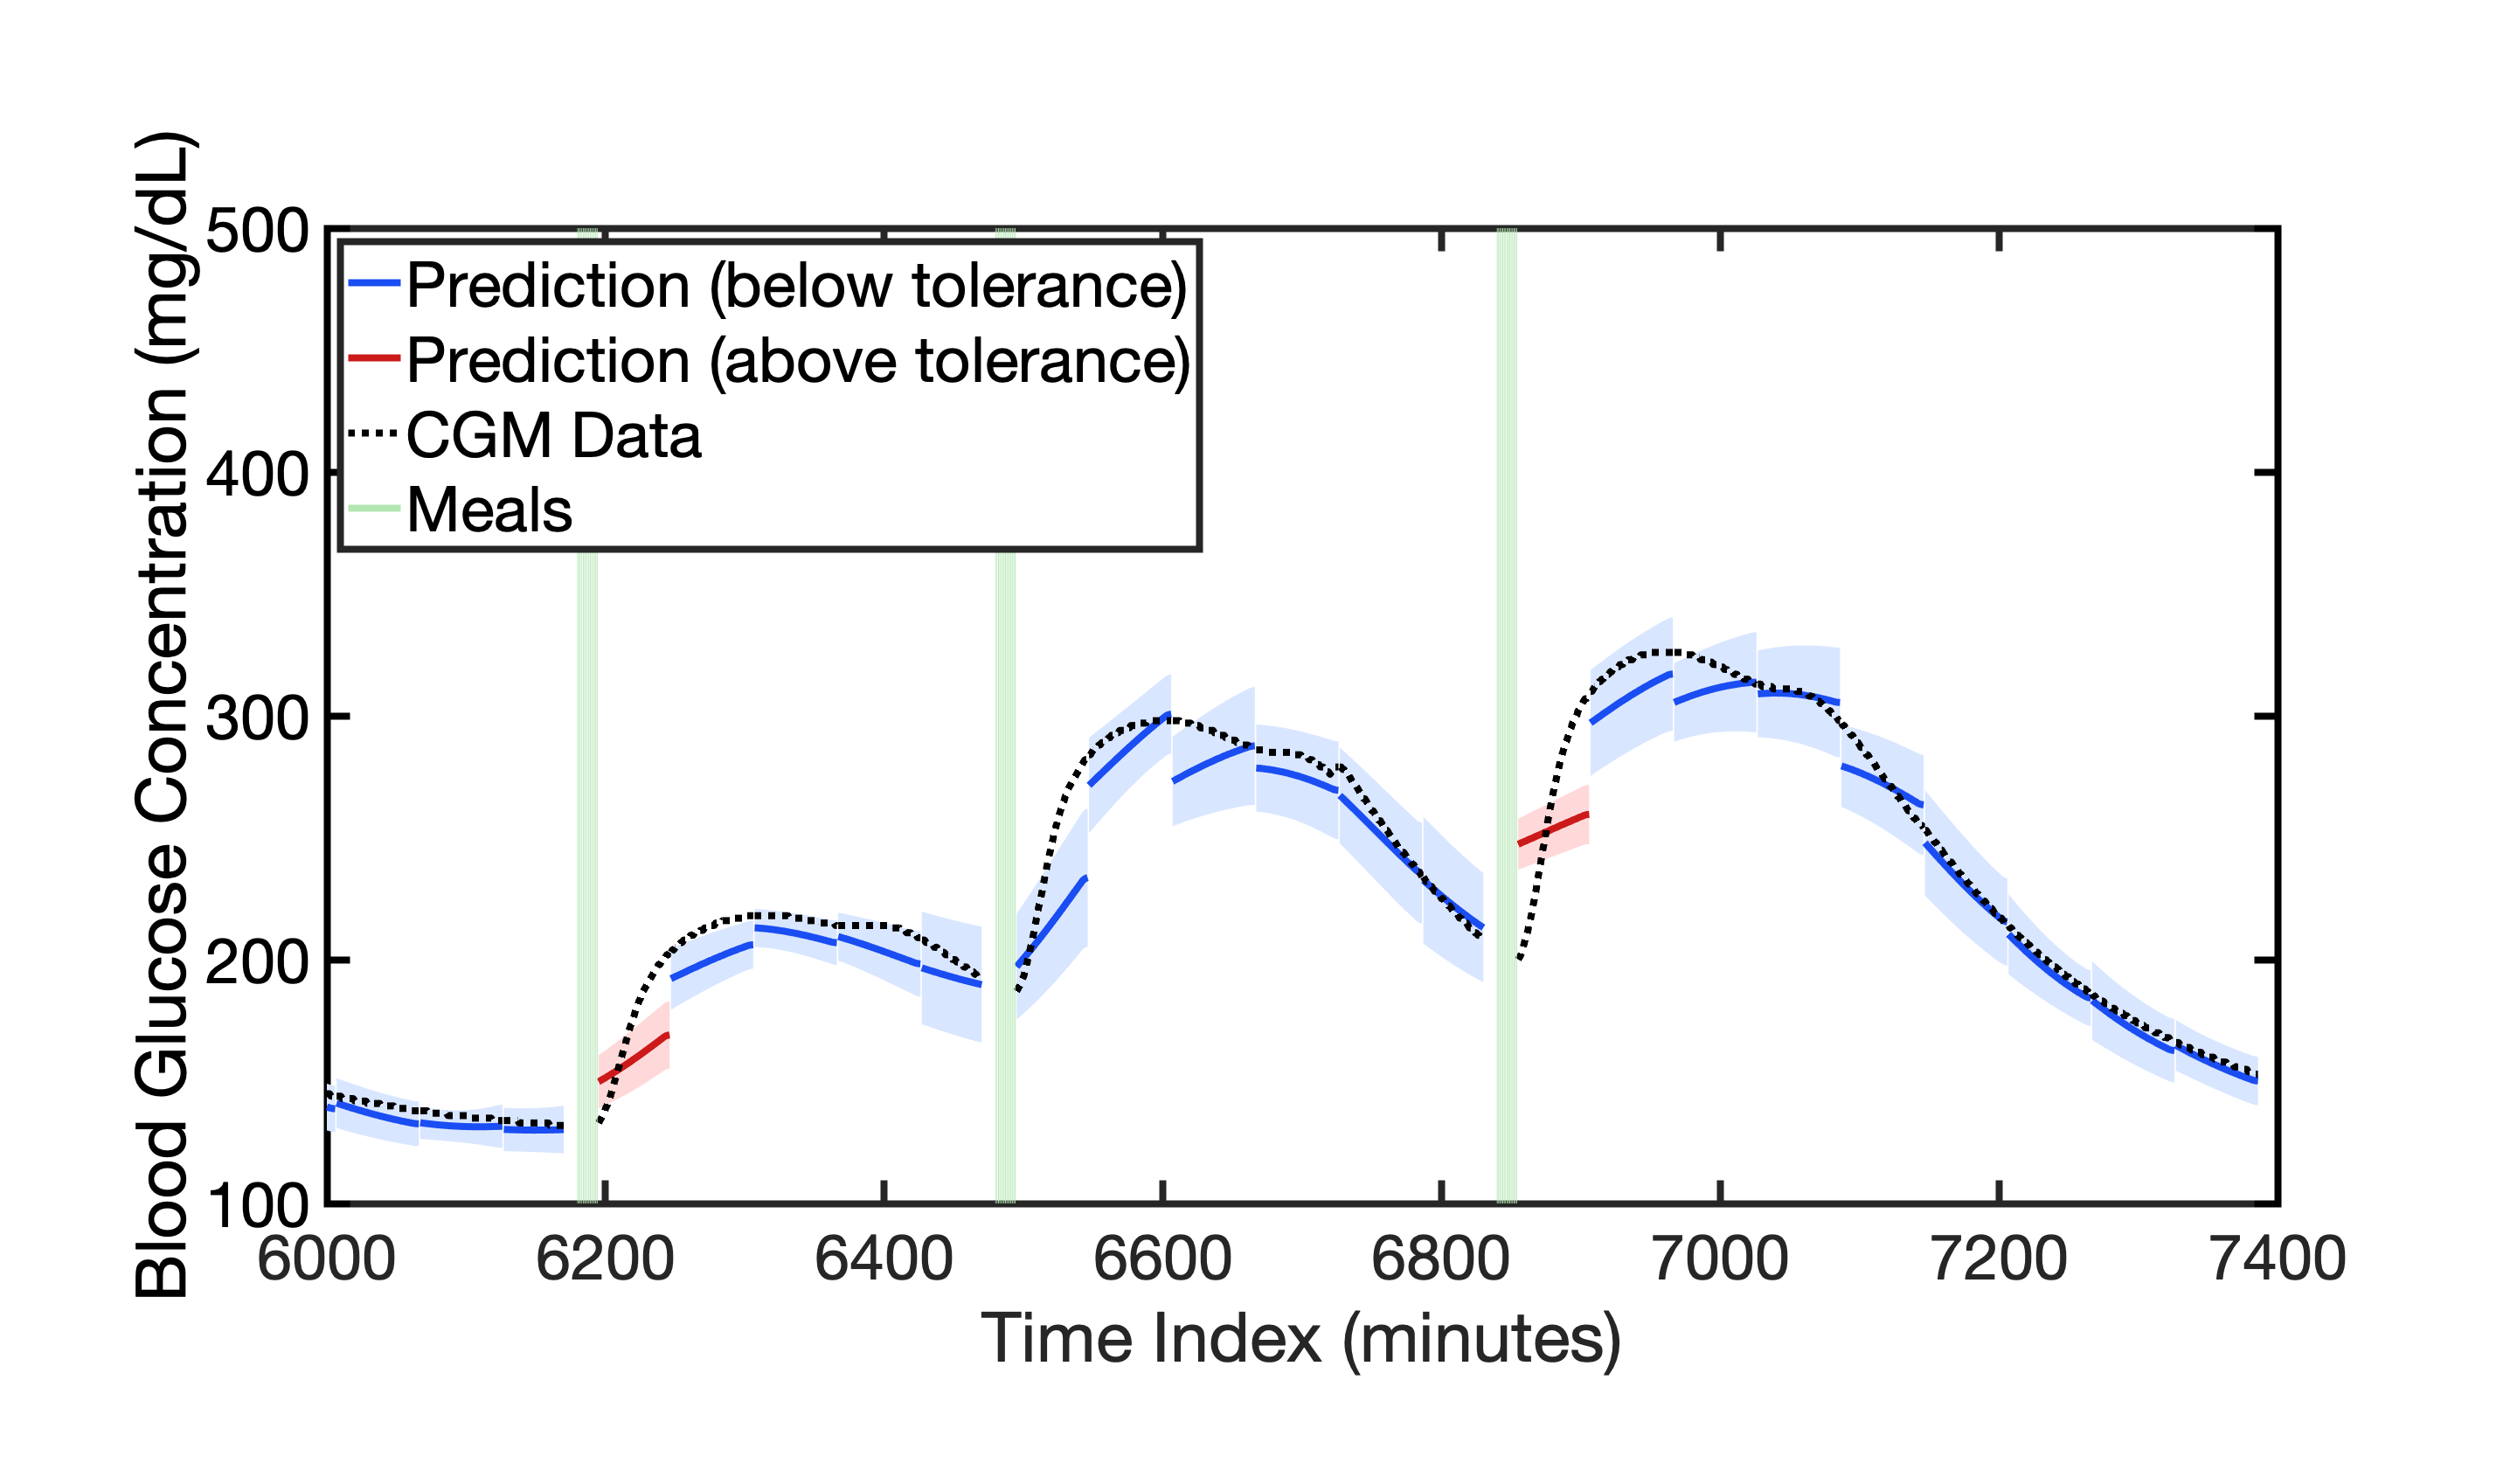
\includegraphics[width=\linewidth]{Figures/Part B/cat3/p1_c3.png}
  \caption*{(a)}
\end{minipage}\hfill
\begin{minipage}[t]{0.48\textwidth}
  \centering
  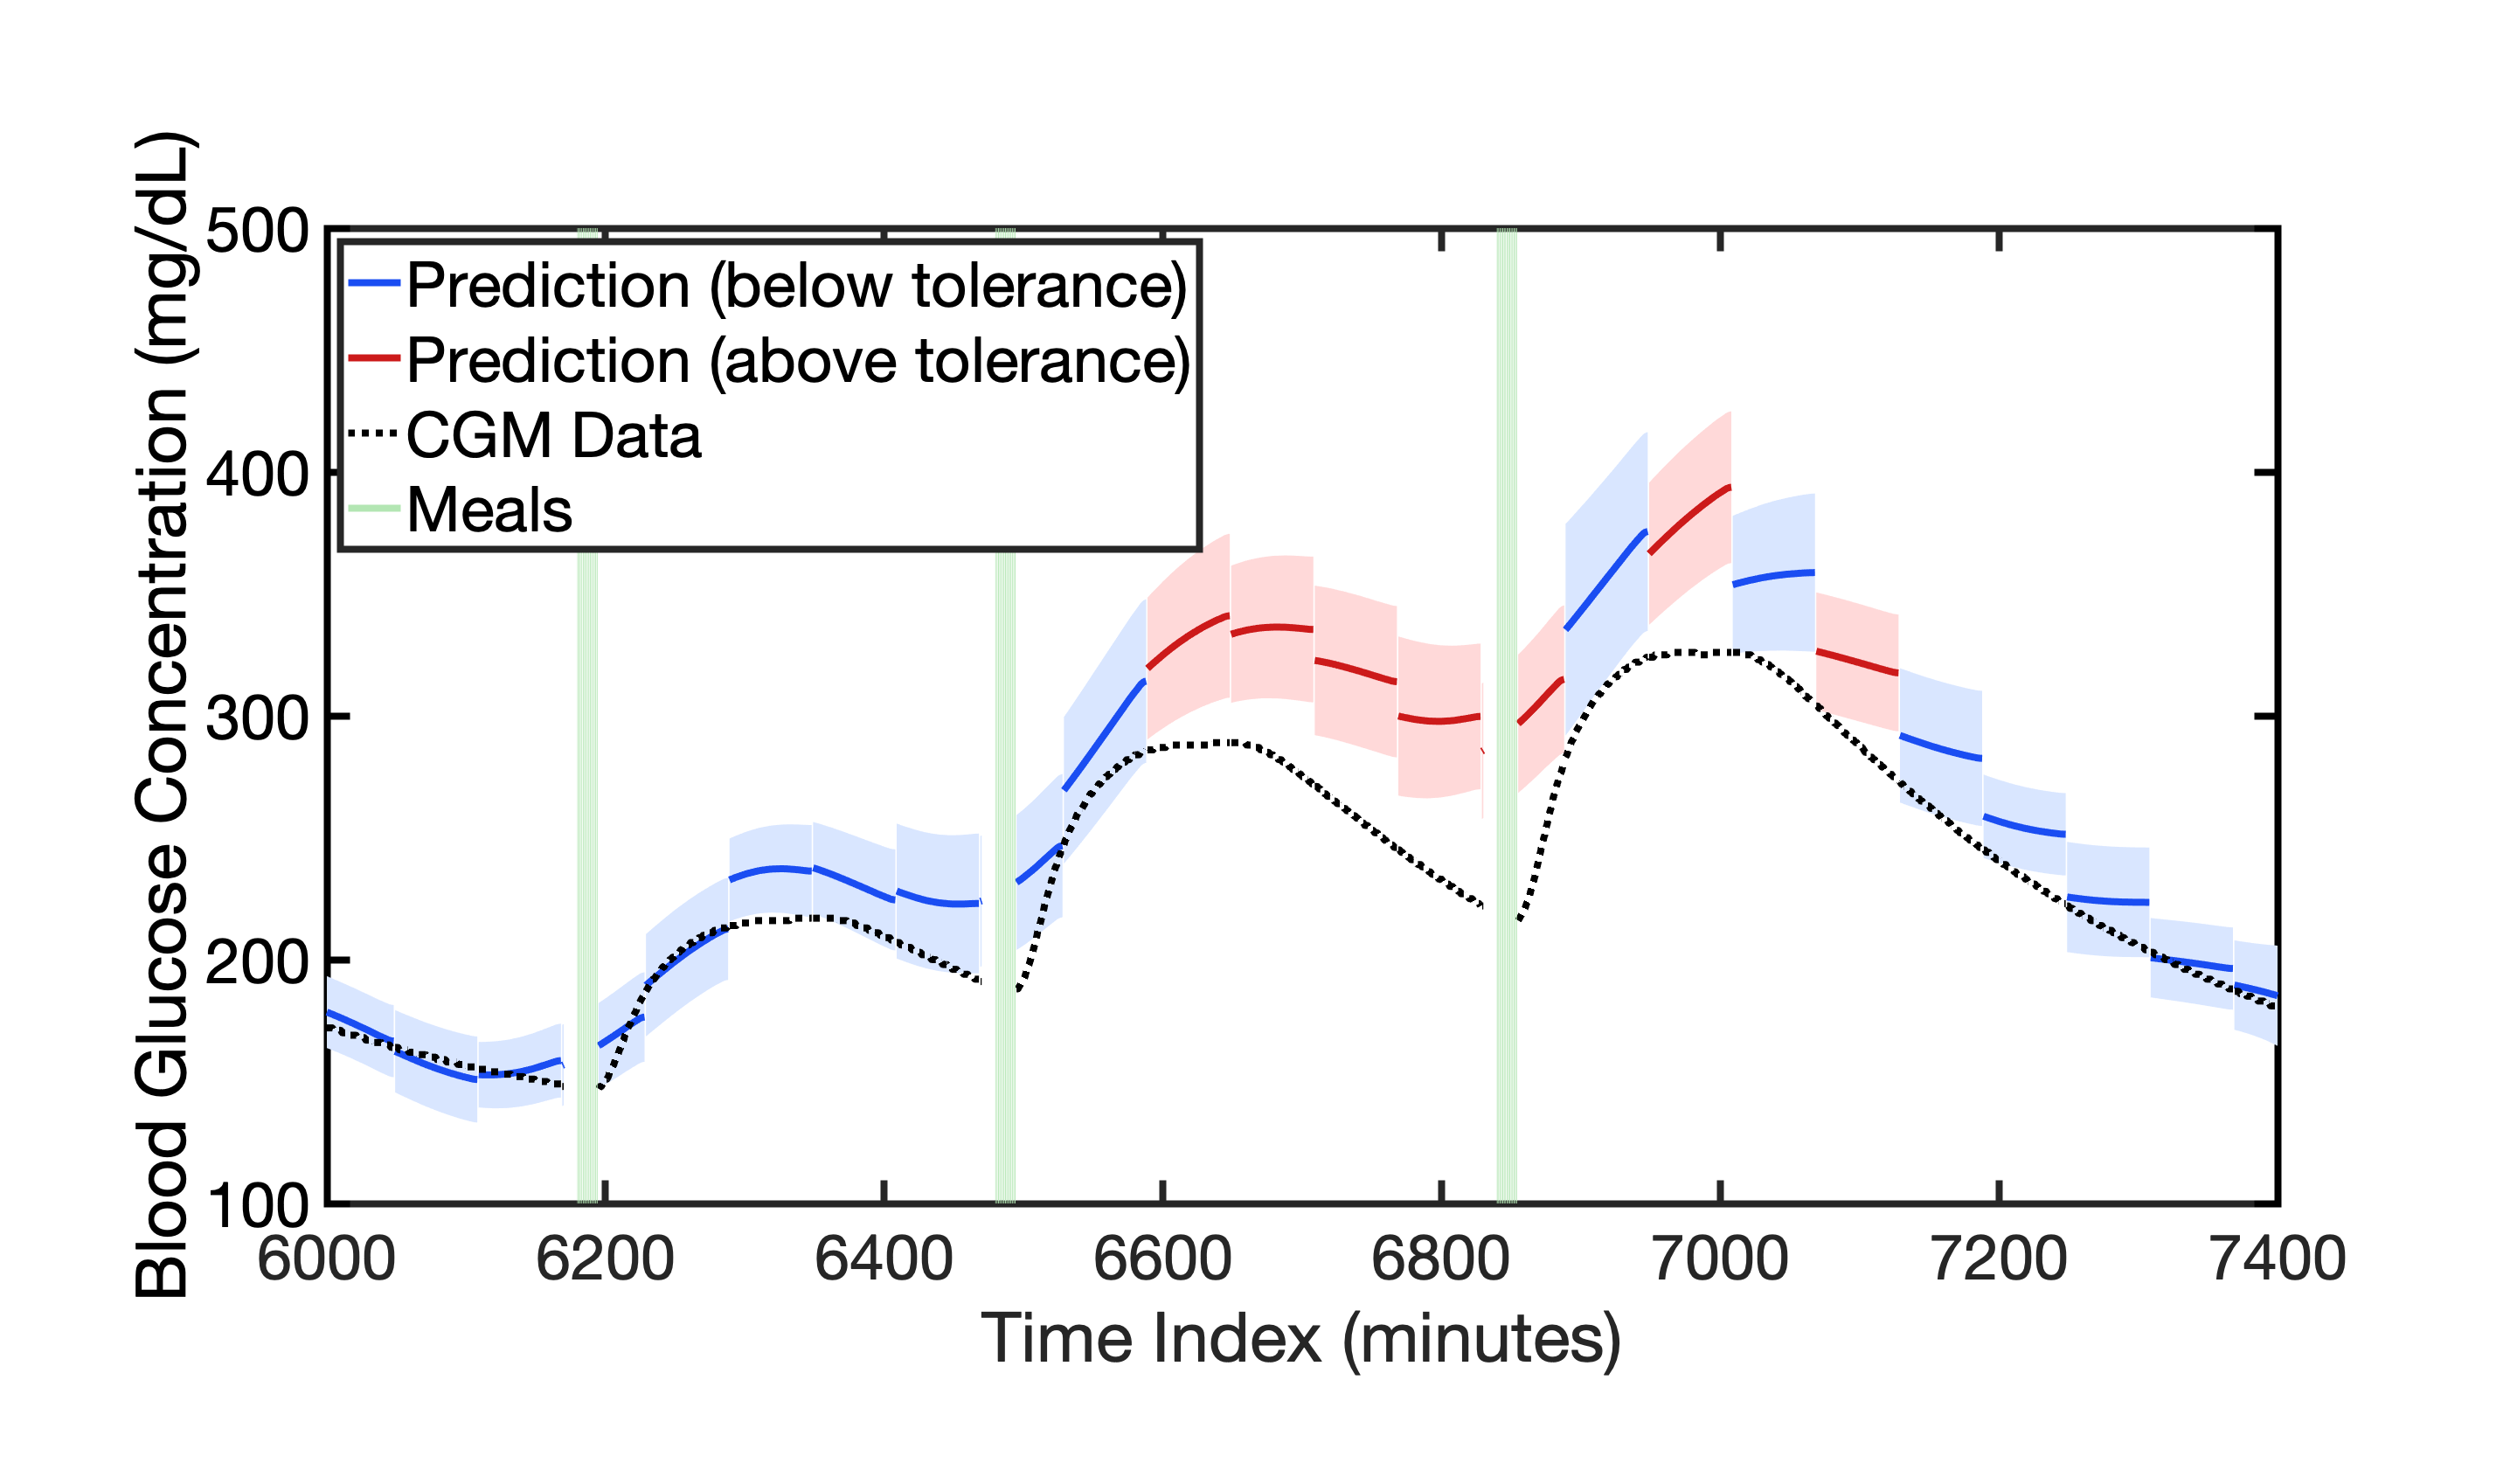
\includegraphics[width=\linewidth]{Figures/Part B/cat3/p4_c3.png}
  \caption*{(b)}
\end{minipage}

\caption{(a) Patient 1 from fold 3, Architecture: $Cat_3Arch_{10}$, and (b) Patient 4 from fold 4, Architecture: $Cat_3Arch_4$}
\label{fig:pred_cat3}
\end{figure}


    
\end{itemize}


%========================================================
%++++++++++++++++++++++++++++++++++++++++++++++++++++++++++++++++++++++++
\subsubsection{Level-wise architecture discovery results}

\paragraph{Capacity Level 1 ($l=1$)}
The lowest-capacity TCN candidates with less than $3 \times 10^4$ parameters, that still satisfy the receptive-field feasibility constraints, are in Level~1.
As shown in Figure \ref{fig:level1_plausibility}, model evidence is not uniformly distributed within this level and it concentrates on a small subset of architectures in each held-out validation fold. 
Despite this, none of the Level~1 architectures satisfy the validation criterion. As illustrated in Figure~\ref{fig:cat1-pred}, predictions on held-out subjects frequently violate the NLPD tolerance across one-hour windows (shown in red). These failures indicate that, although some architectures are favored by the population-based training data, their representational capacity is insufficient to generalize to subject-specific glucose dynamics. Consequently, EVIDENT rejects Level~1 and proceeds to the next capacity level.


\begin{figure}[!ht]
\centering
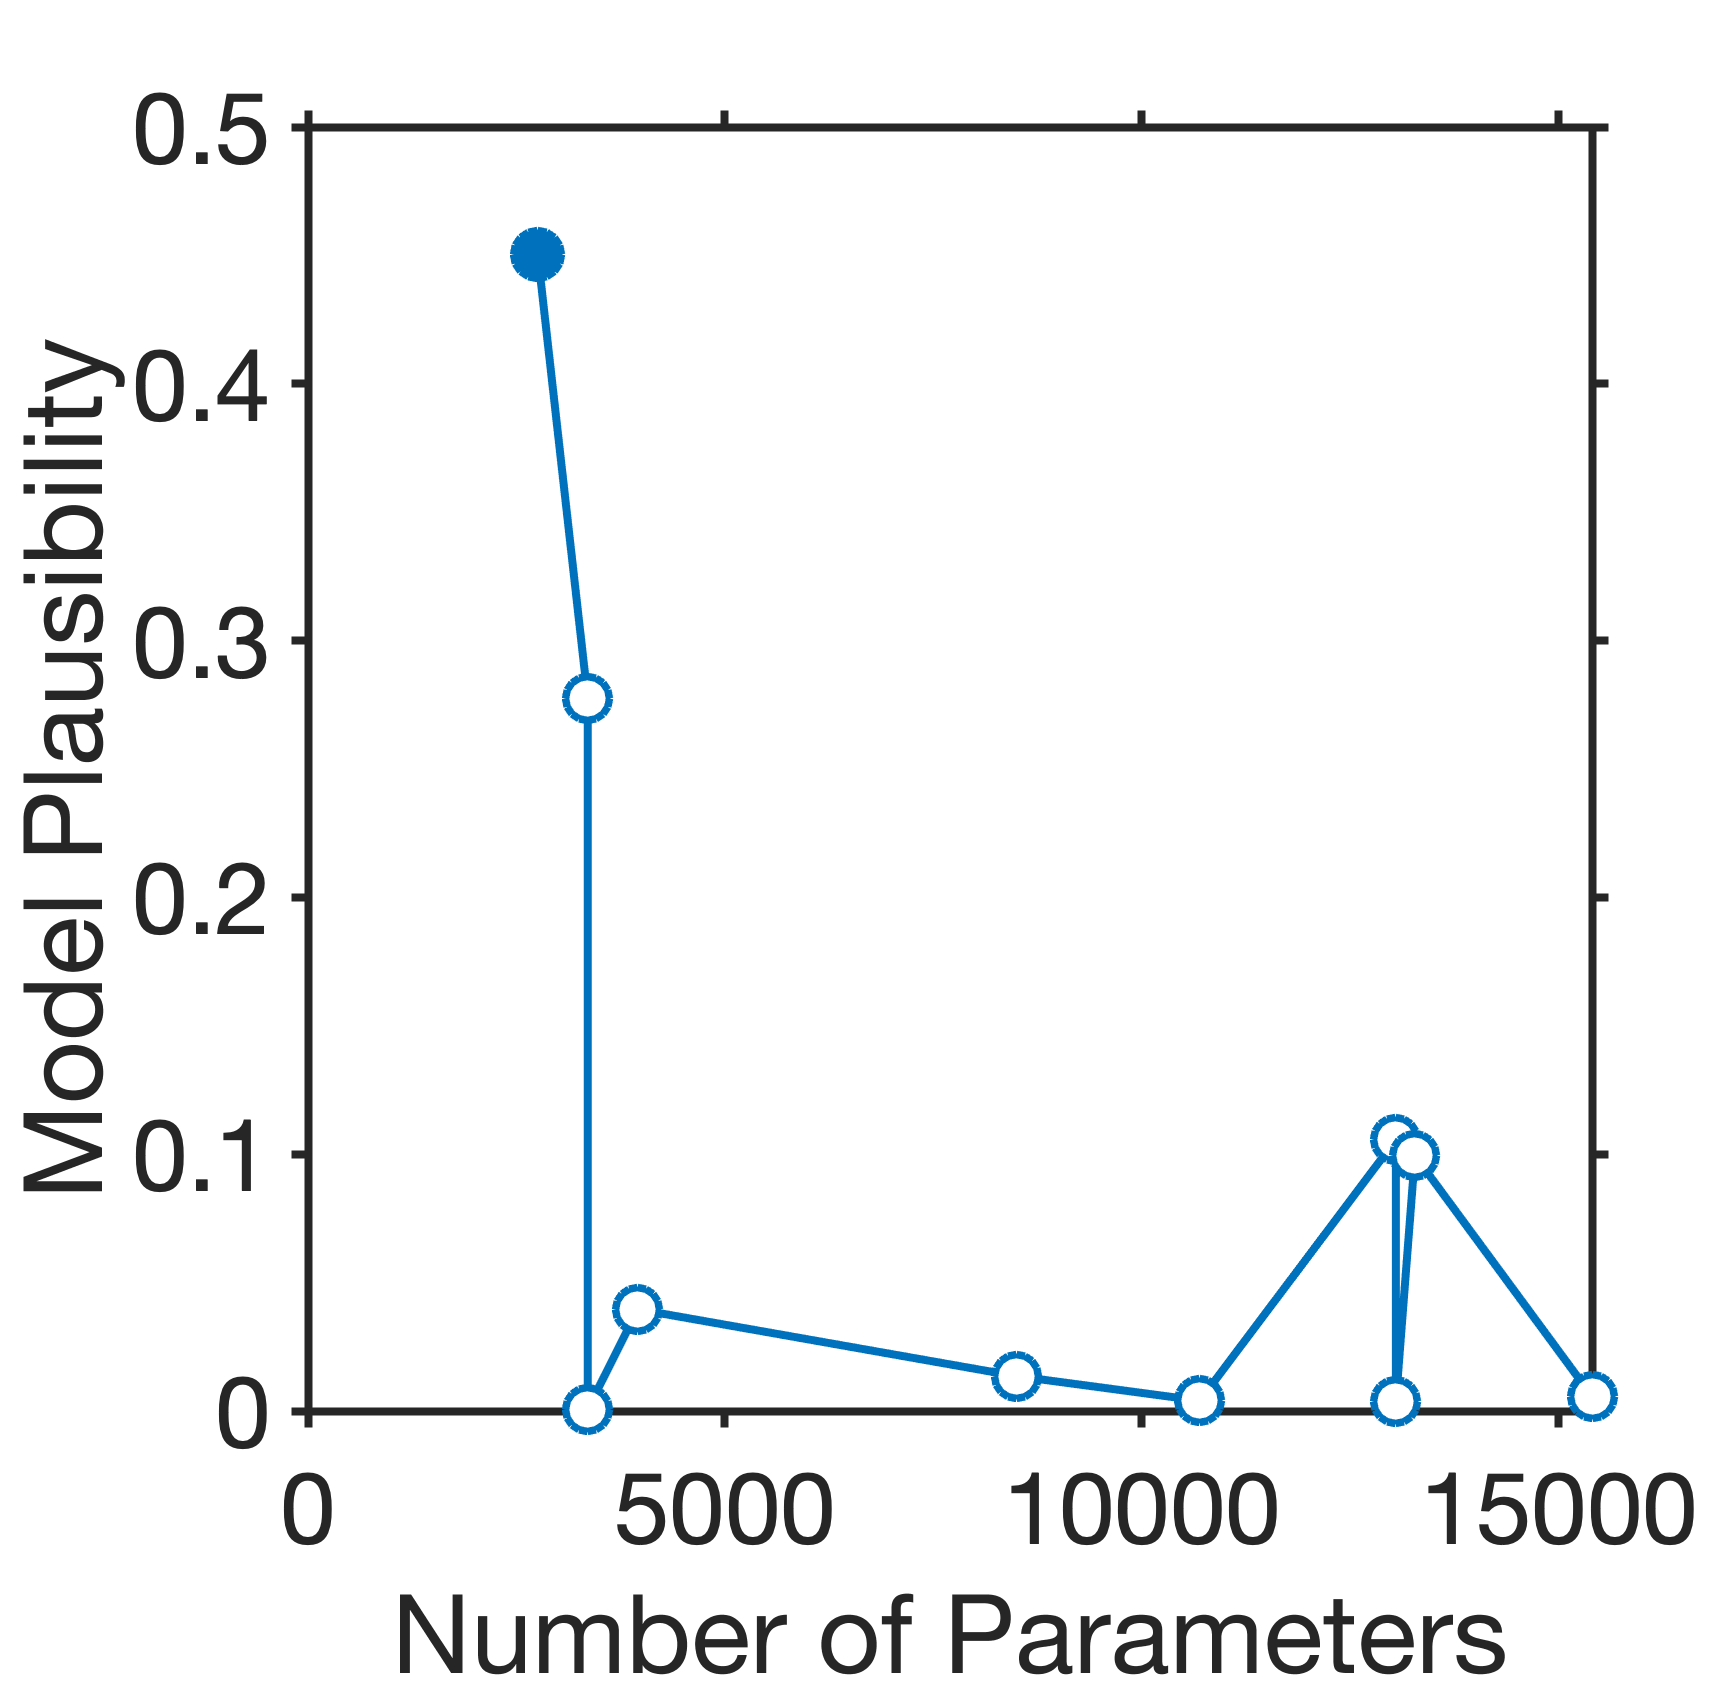
\includegraphics[width=0.19\textwidth]{Figures/Part B/cat1/fold1.png}\hfill
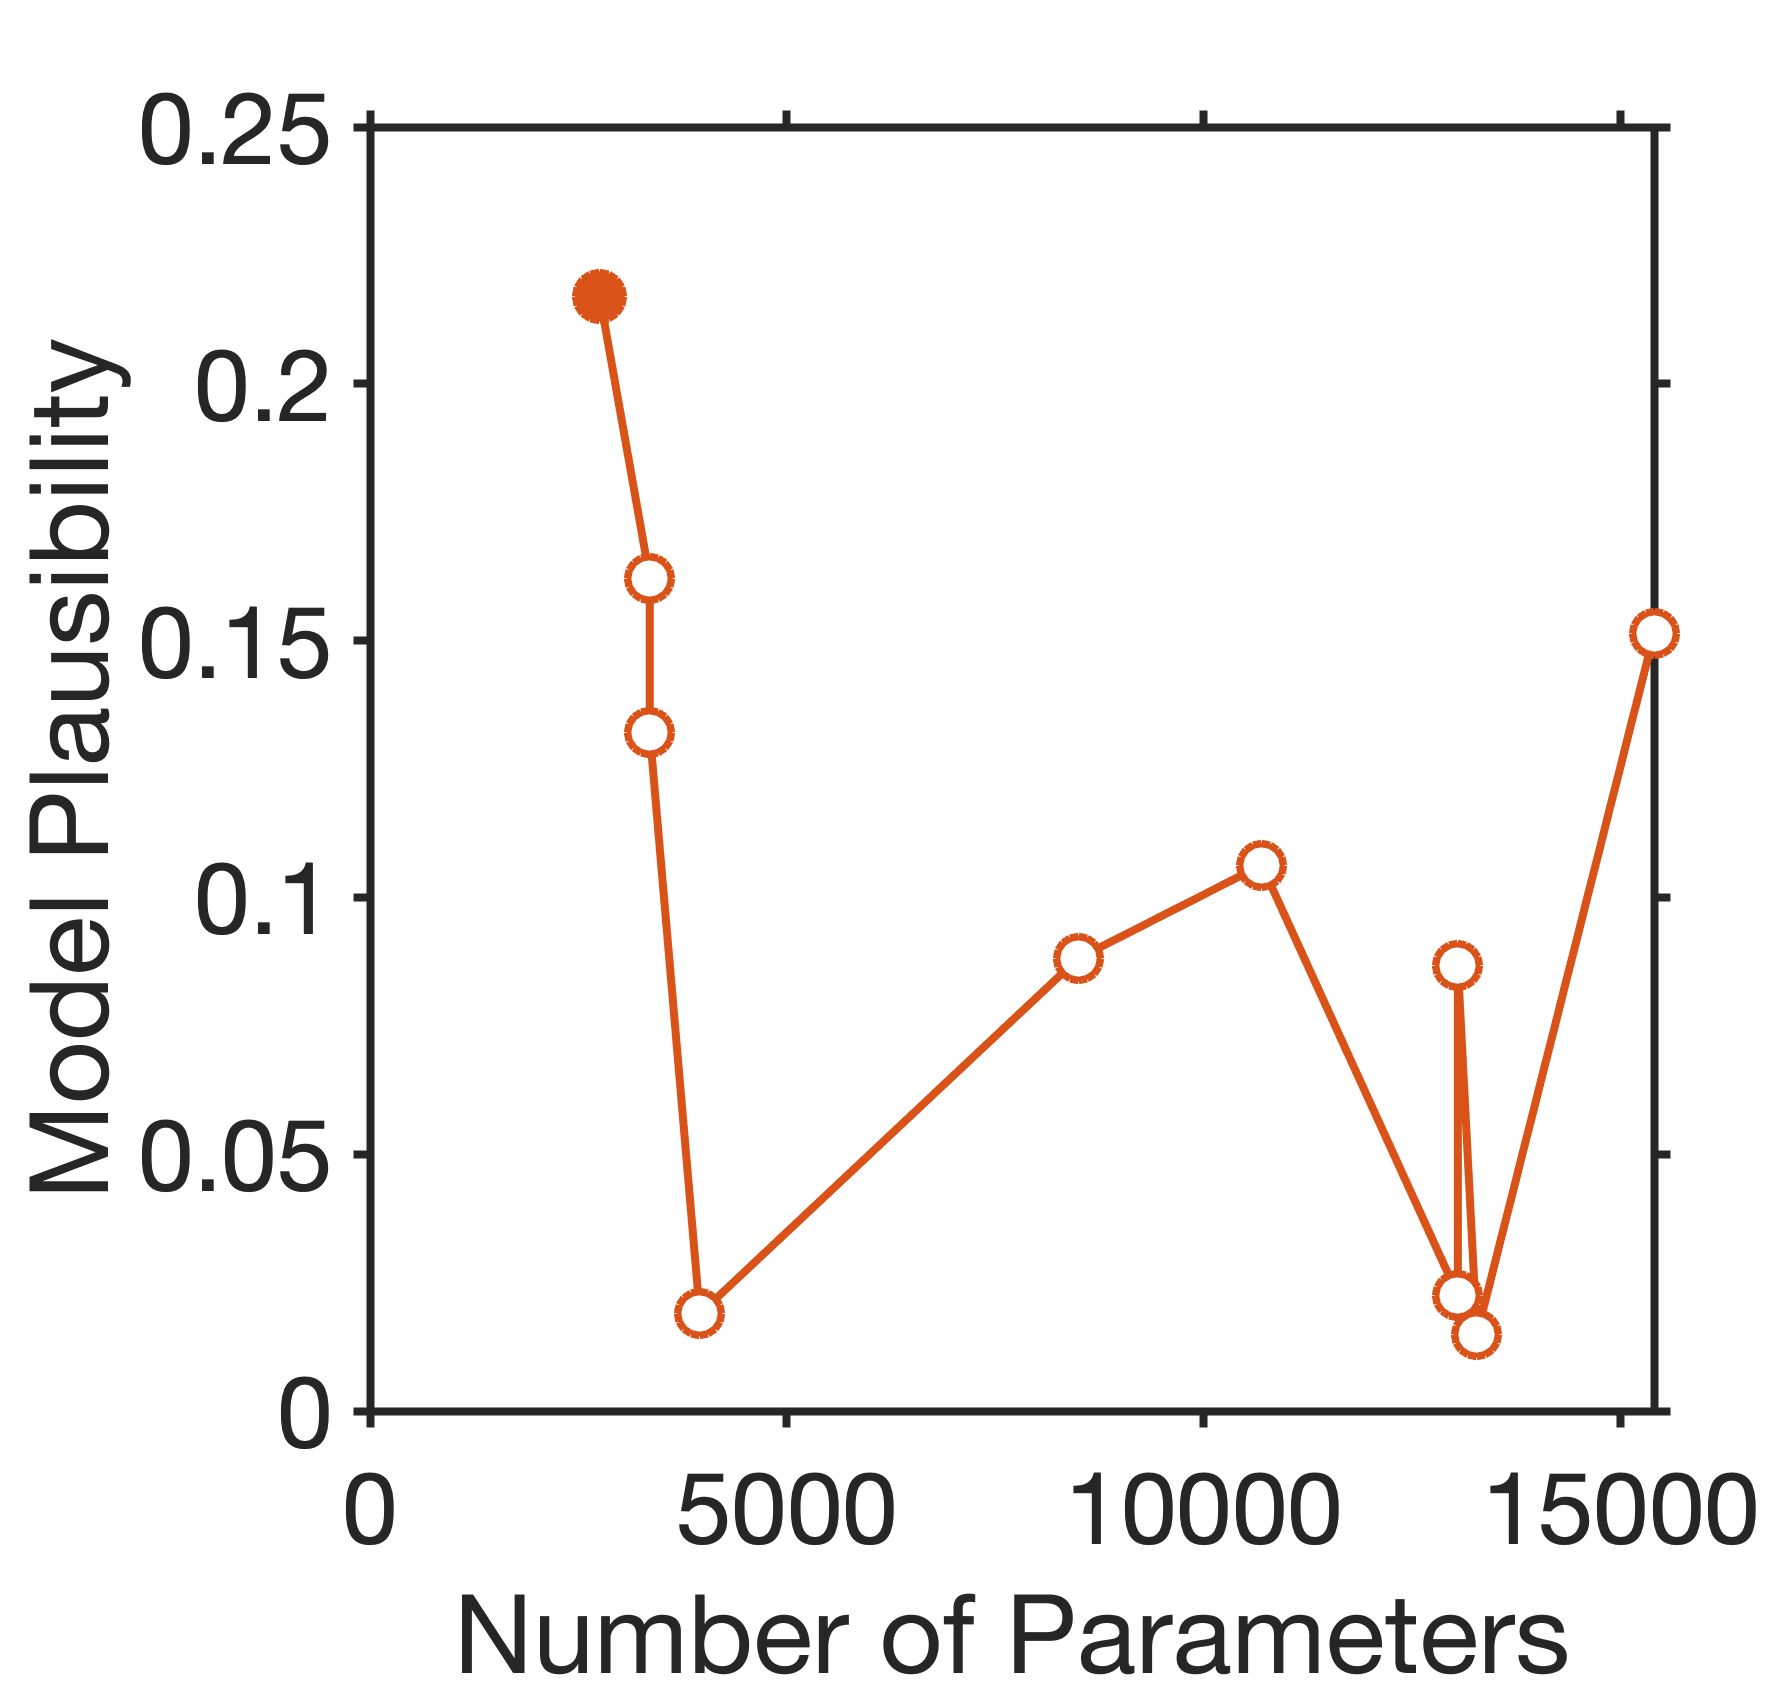
\includegraphics[width=0.19\textwidth]{Figures/Part B/cat1/fold2.png}\hfill
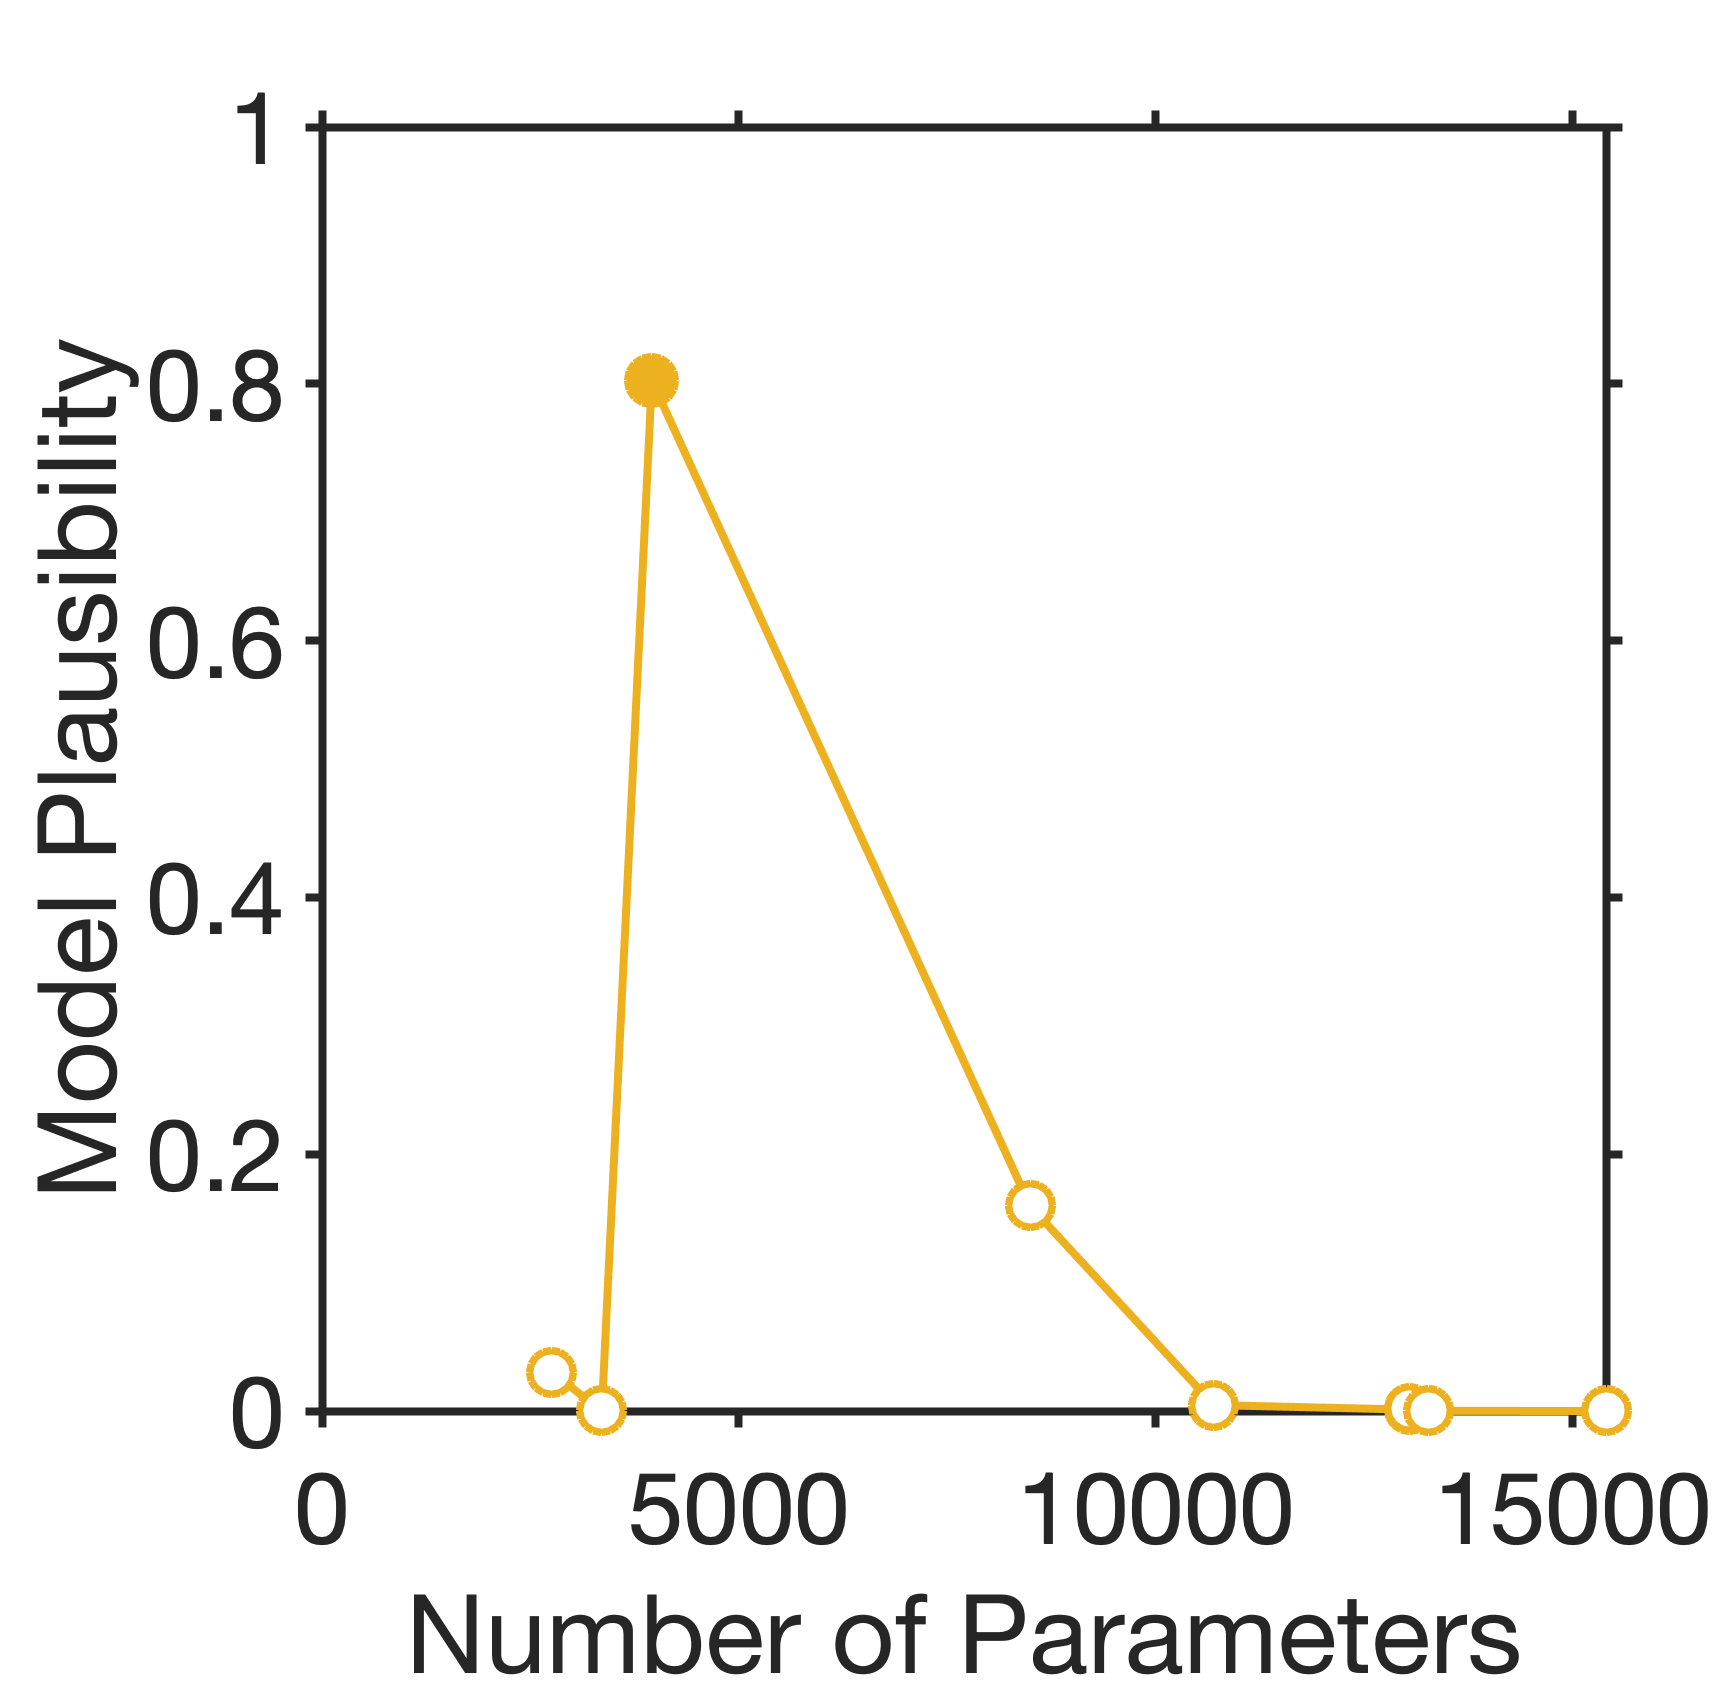
\includegraphics[width=0.19\textwidth]{Figures/Part B/cat1/fold3.png}\hfill
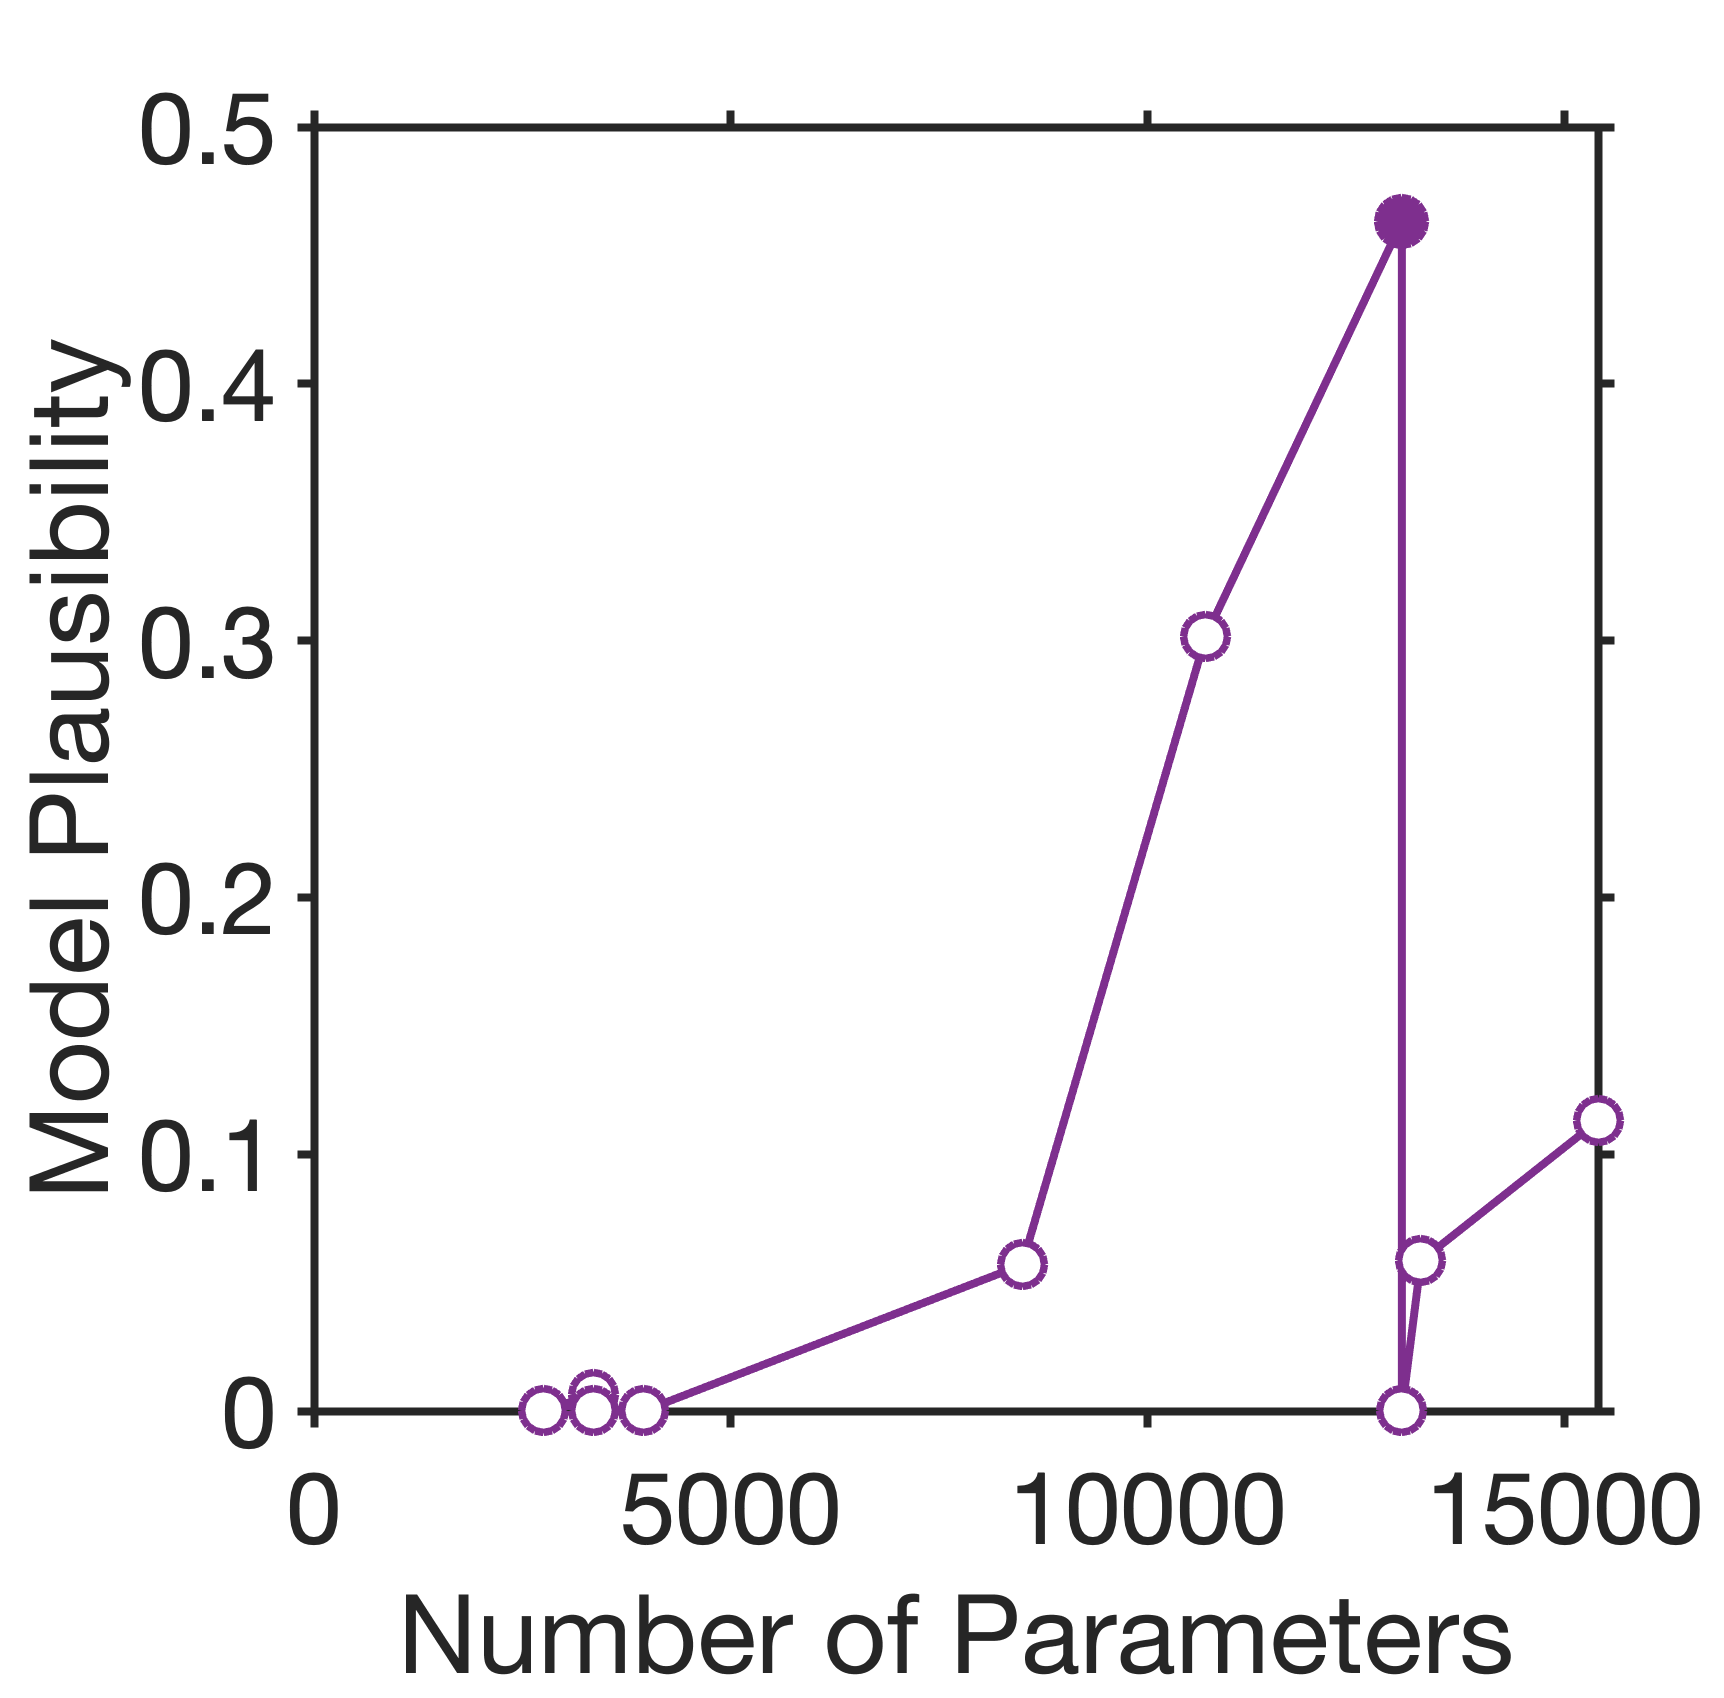
\includegraphics[width=0.19\textwidth]{Figures/Part B/cat1/fold4.png}\hfill
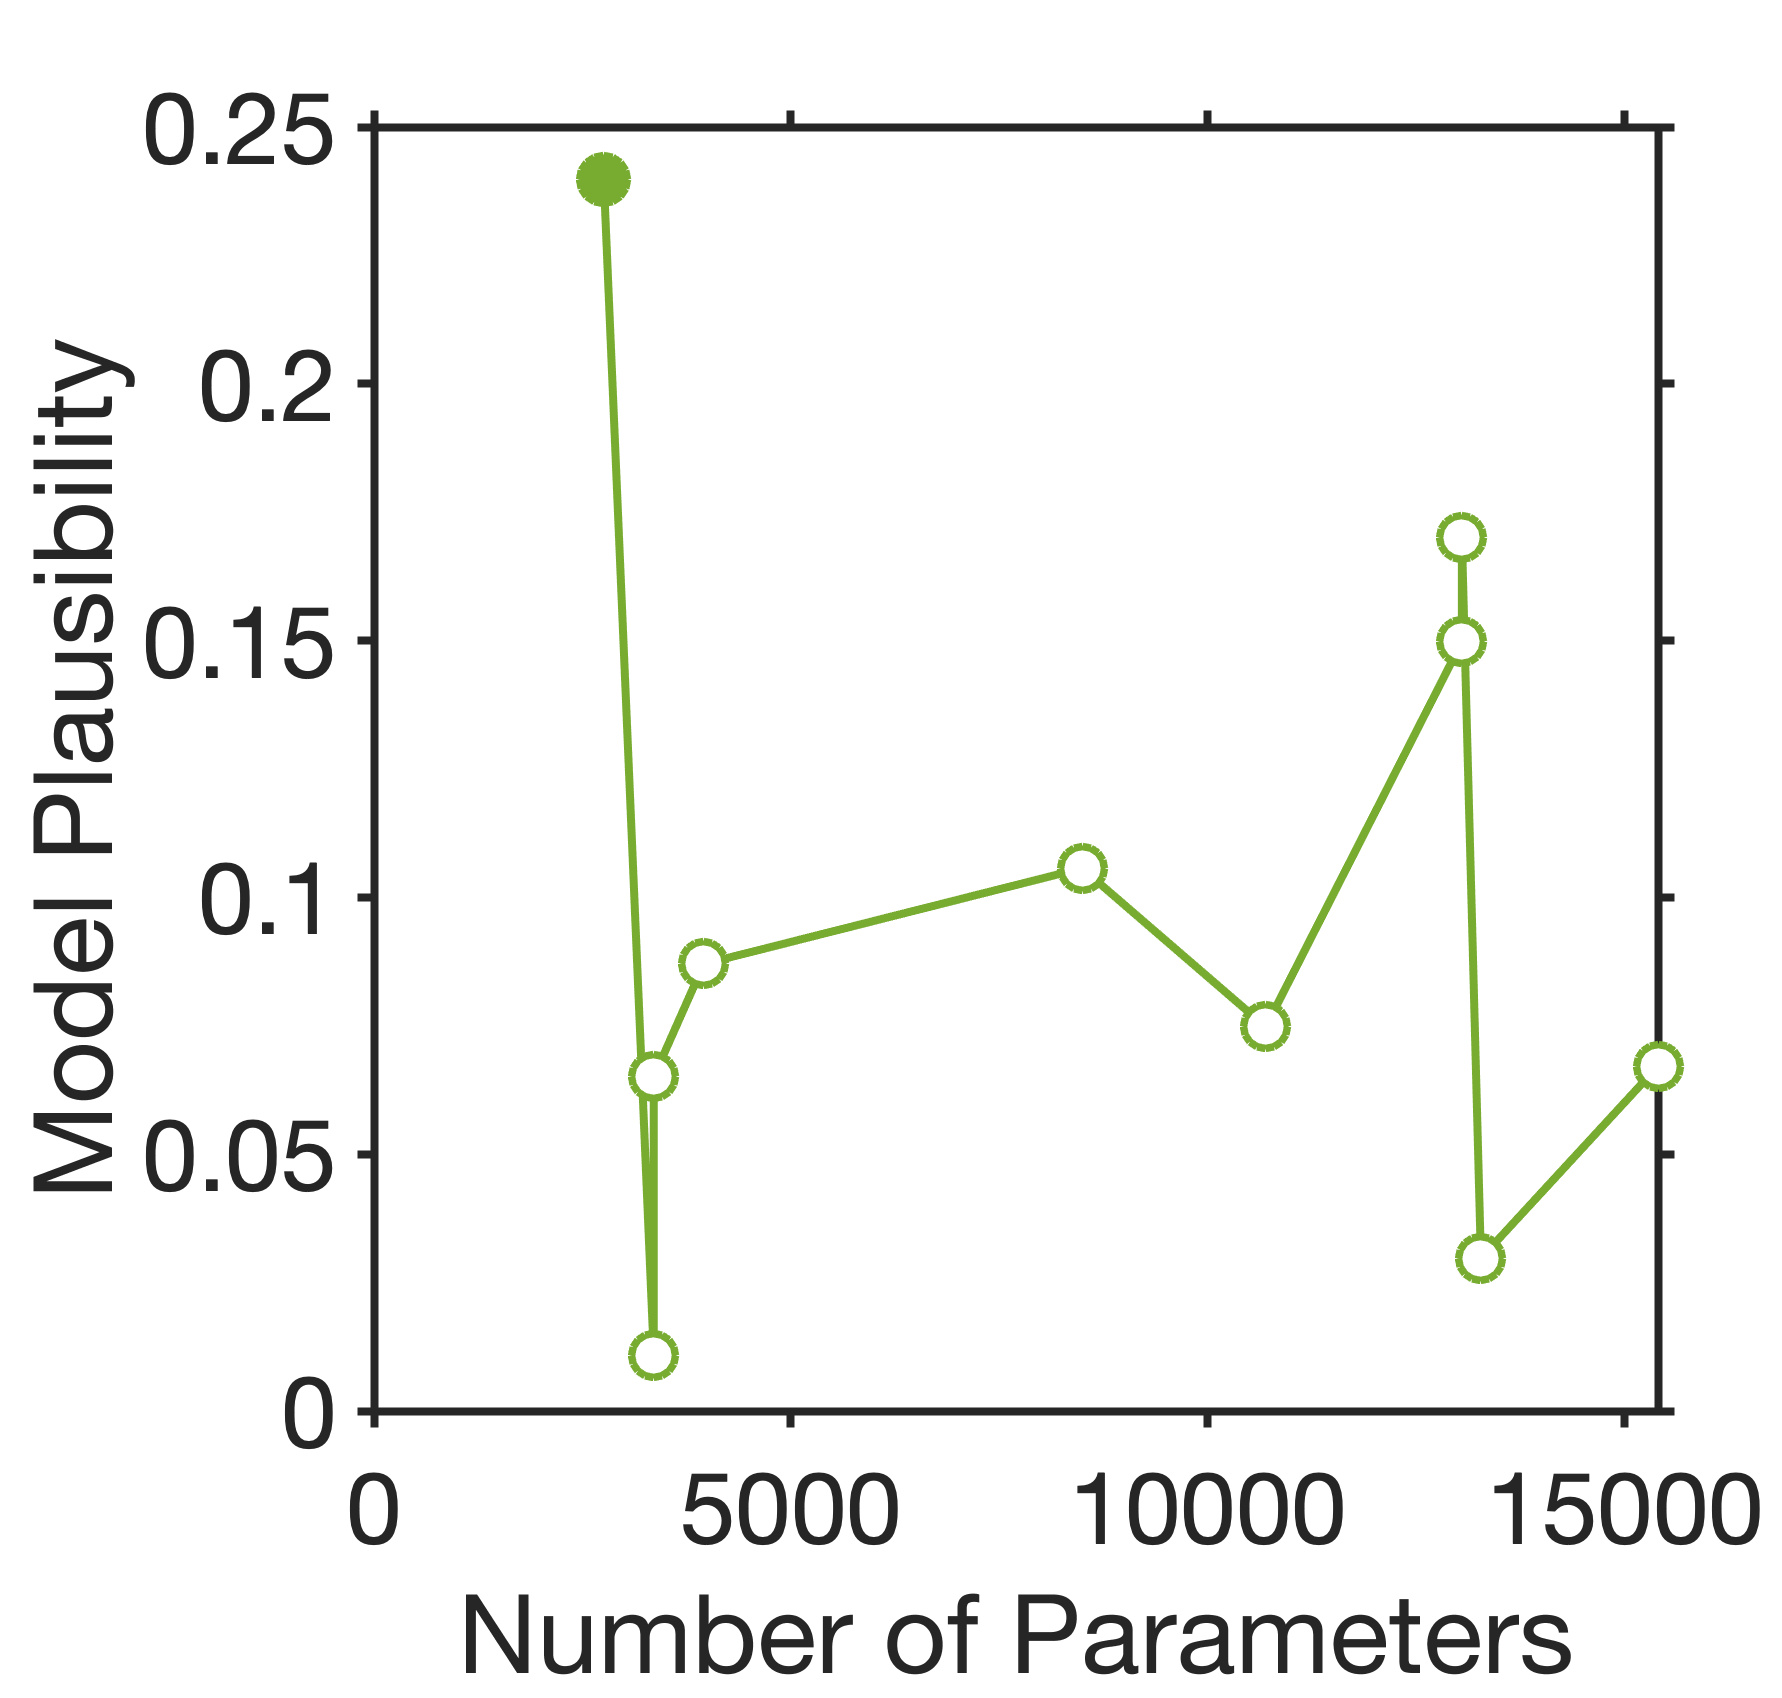
\includegraphics[width=0.19\textwidth]{Figures/Part B/cat1/fold5.png}
\caption{Level~1 architectures: Posterior plausibility $\rho$ versus model size (number of parameters) with identified most plausible architecture $\xi_{\mathrm{plauisble}}$ across validation folds (left to right: folds 1–5).}
\label{fig:level1_plausibility}
\end{figure}


\begin{figure}[!ht]
\centering
\begin{minipage}[t]{0.48\textwidth}
  \centering
  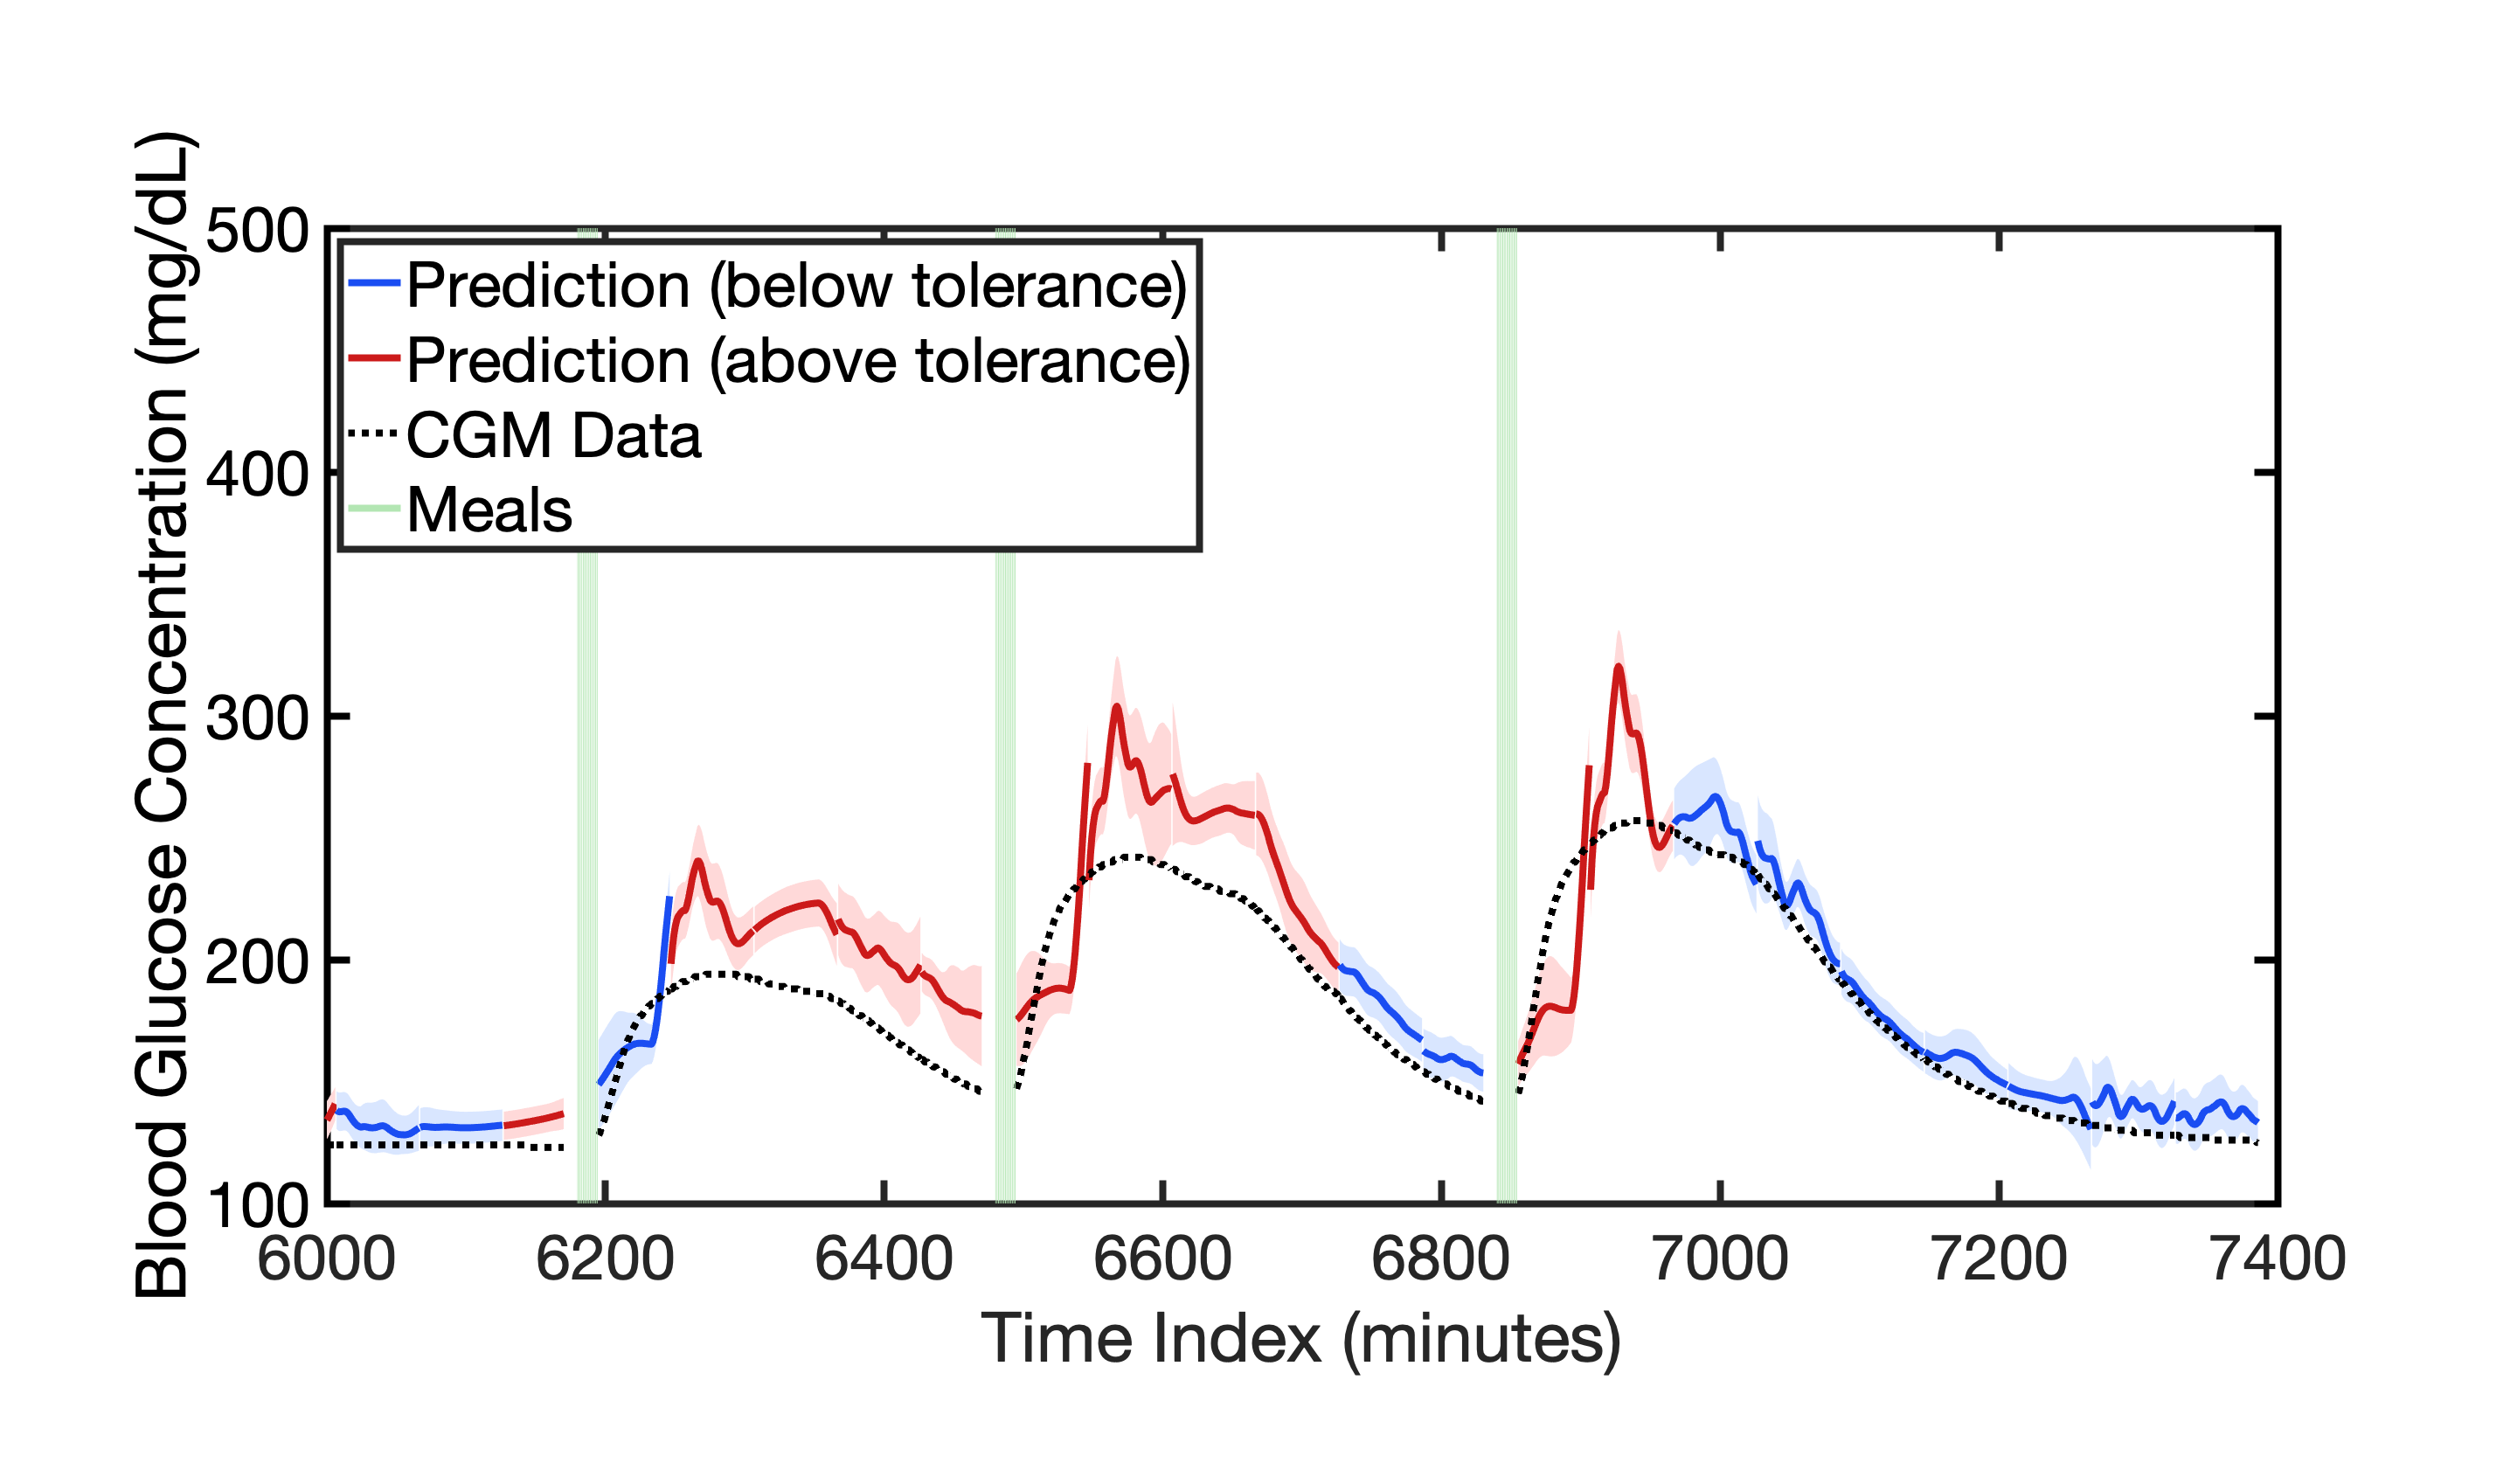
\includegraphics[width=\linewidth]{Figures/Part B/cat1/p2_c1.png}
  \caption*{(a)}
\end{minipage}\hfill
\begin{minipage}[t]{0.48\textwidth}
  \centering
  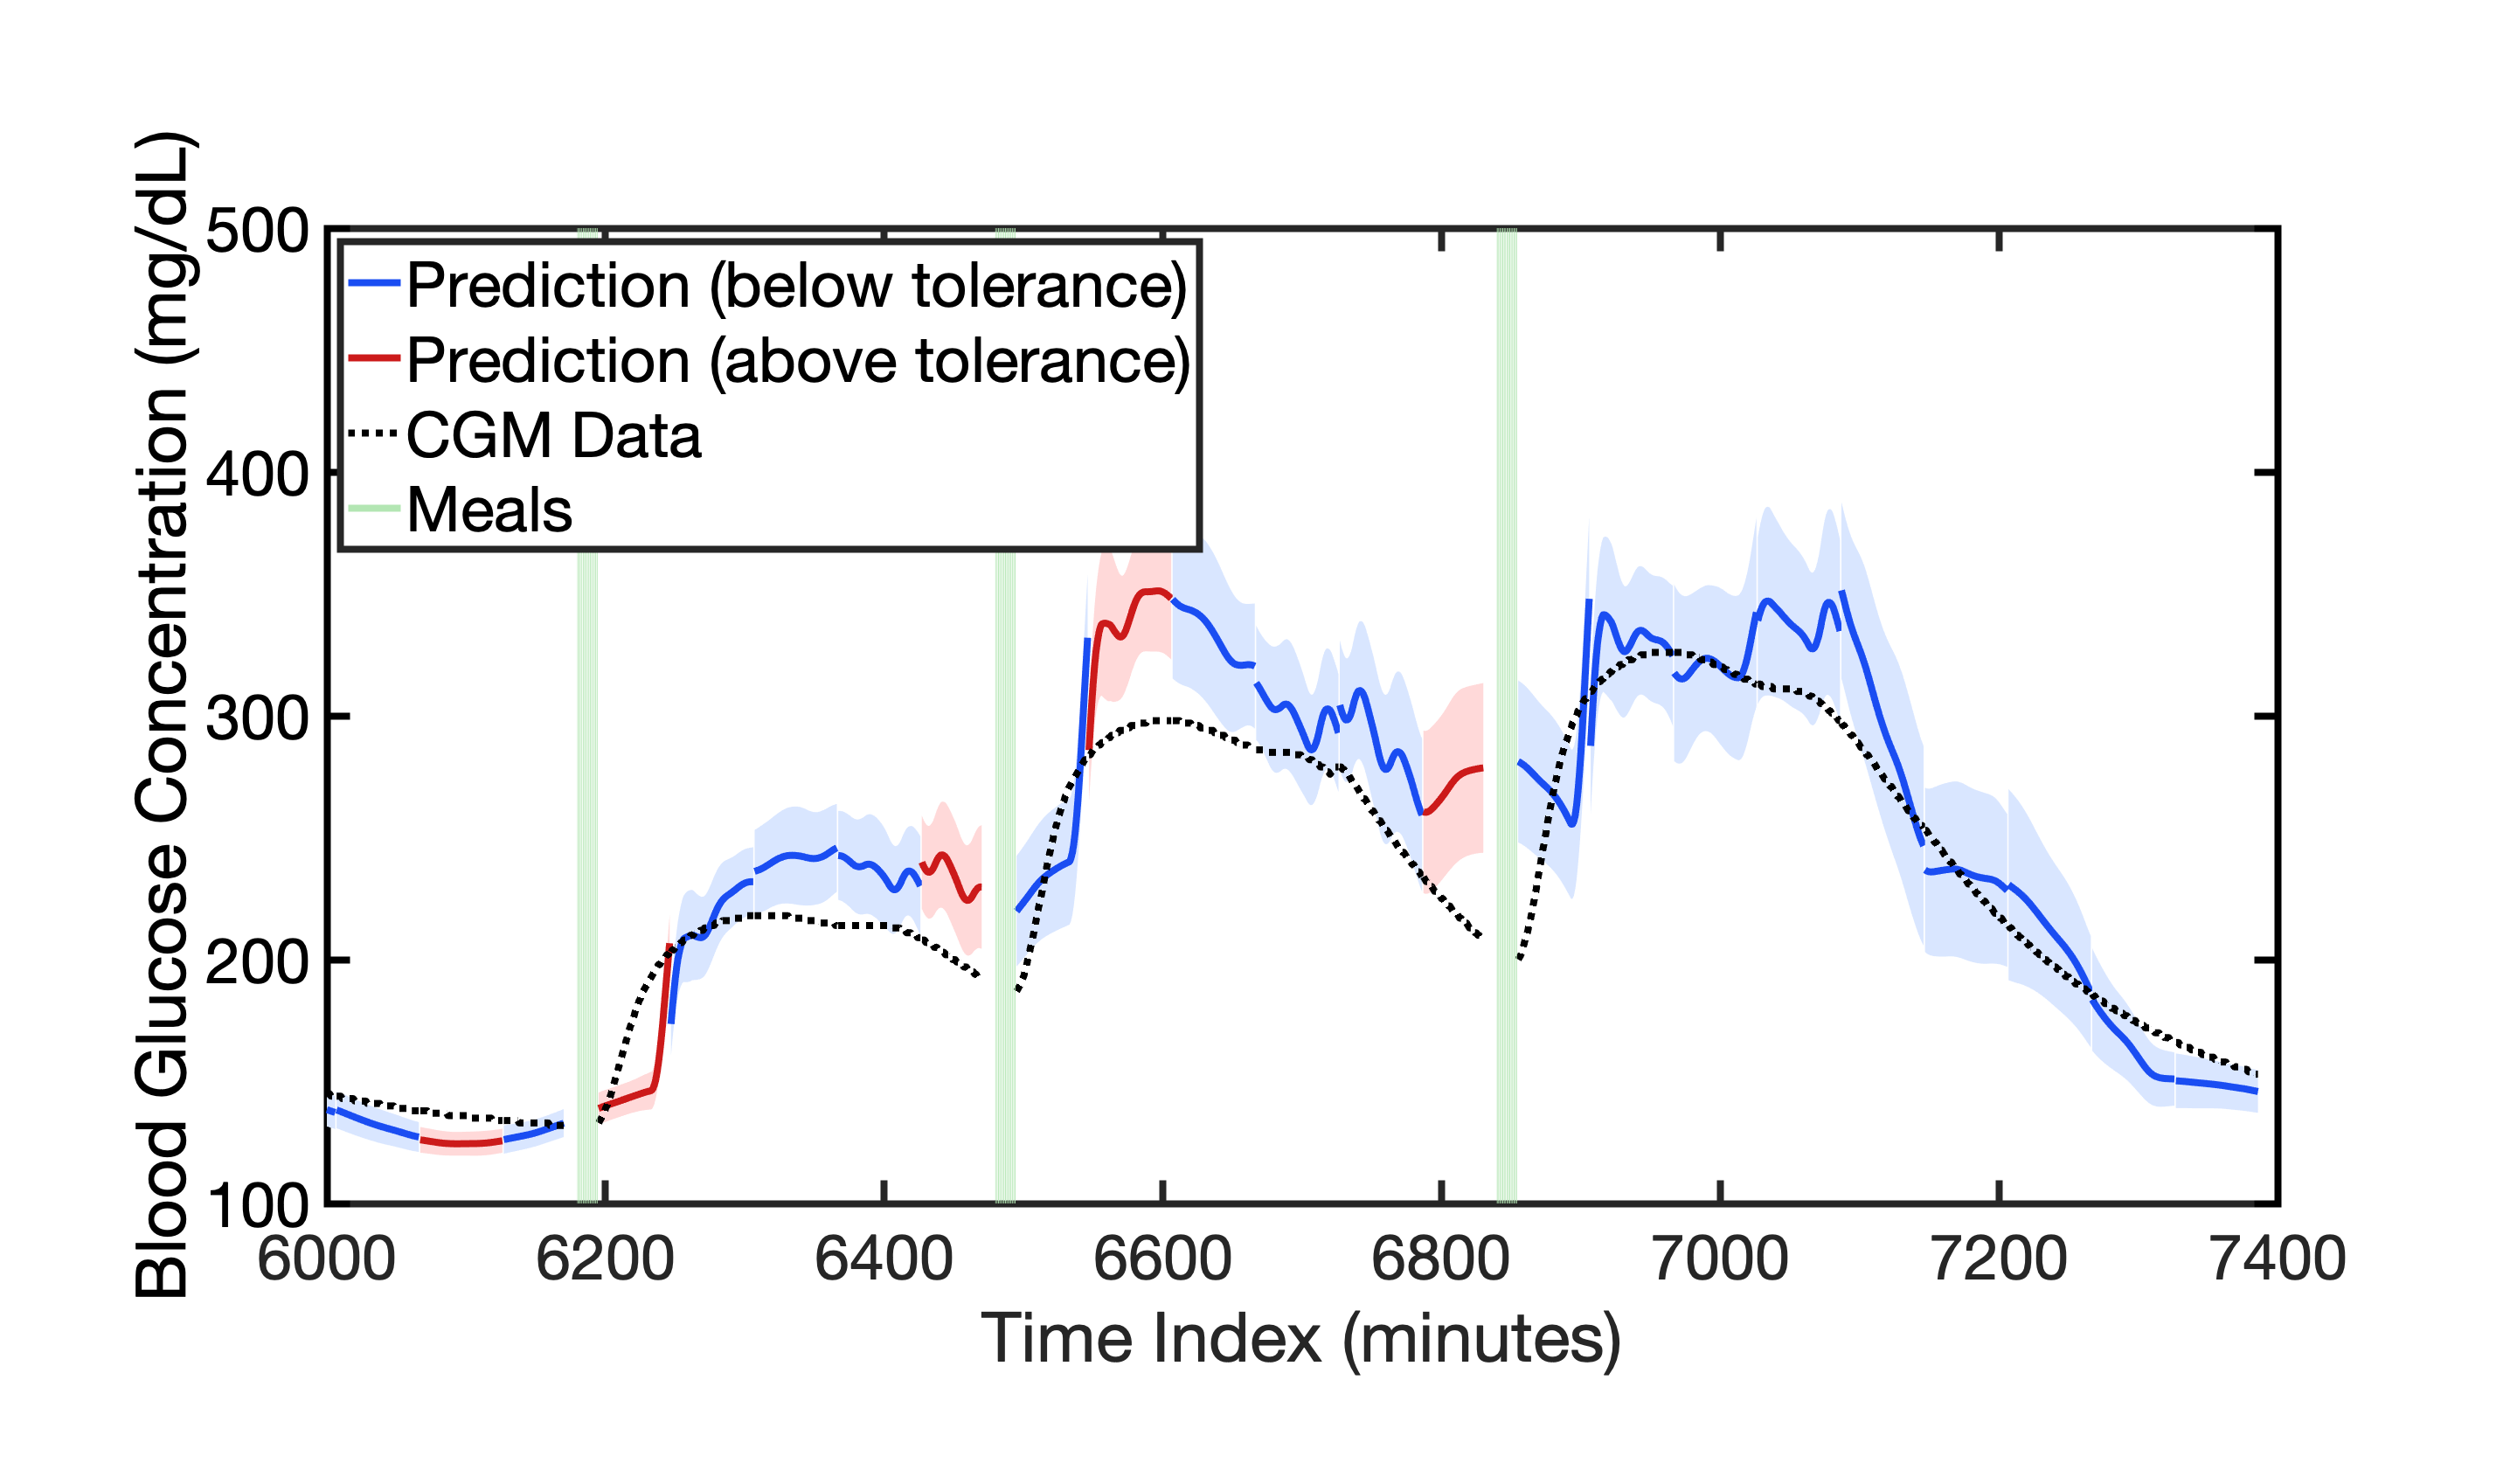
\includegraphics[width=\linewidth]{Figures/Part B/cat1/p1_c1.png}
  \caption*{(b)}
\end{minipage}
\begin{minipage}[t]{0.48\textwidth}
  \centering
  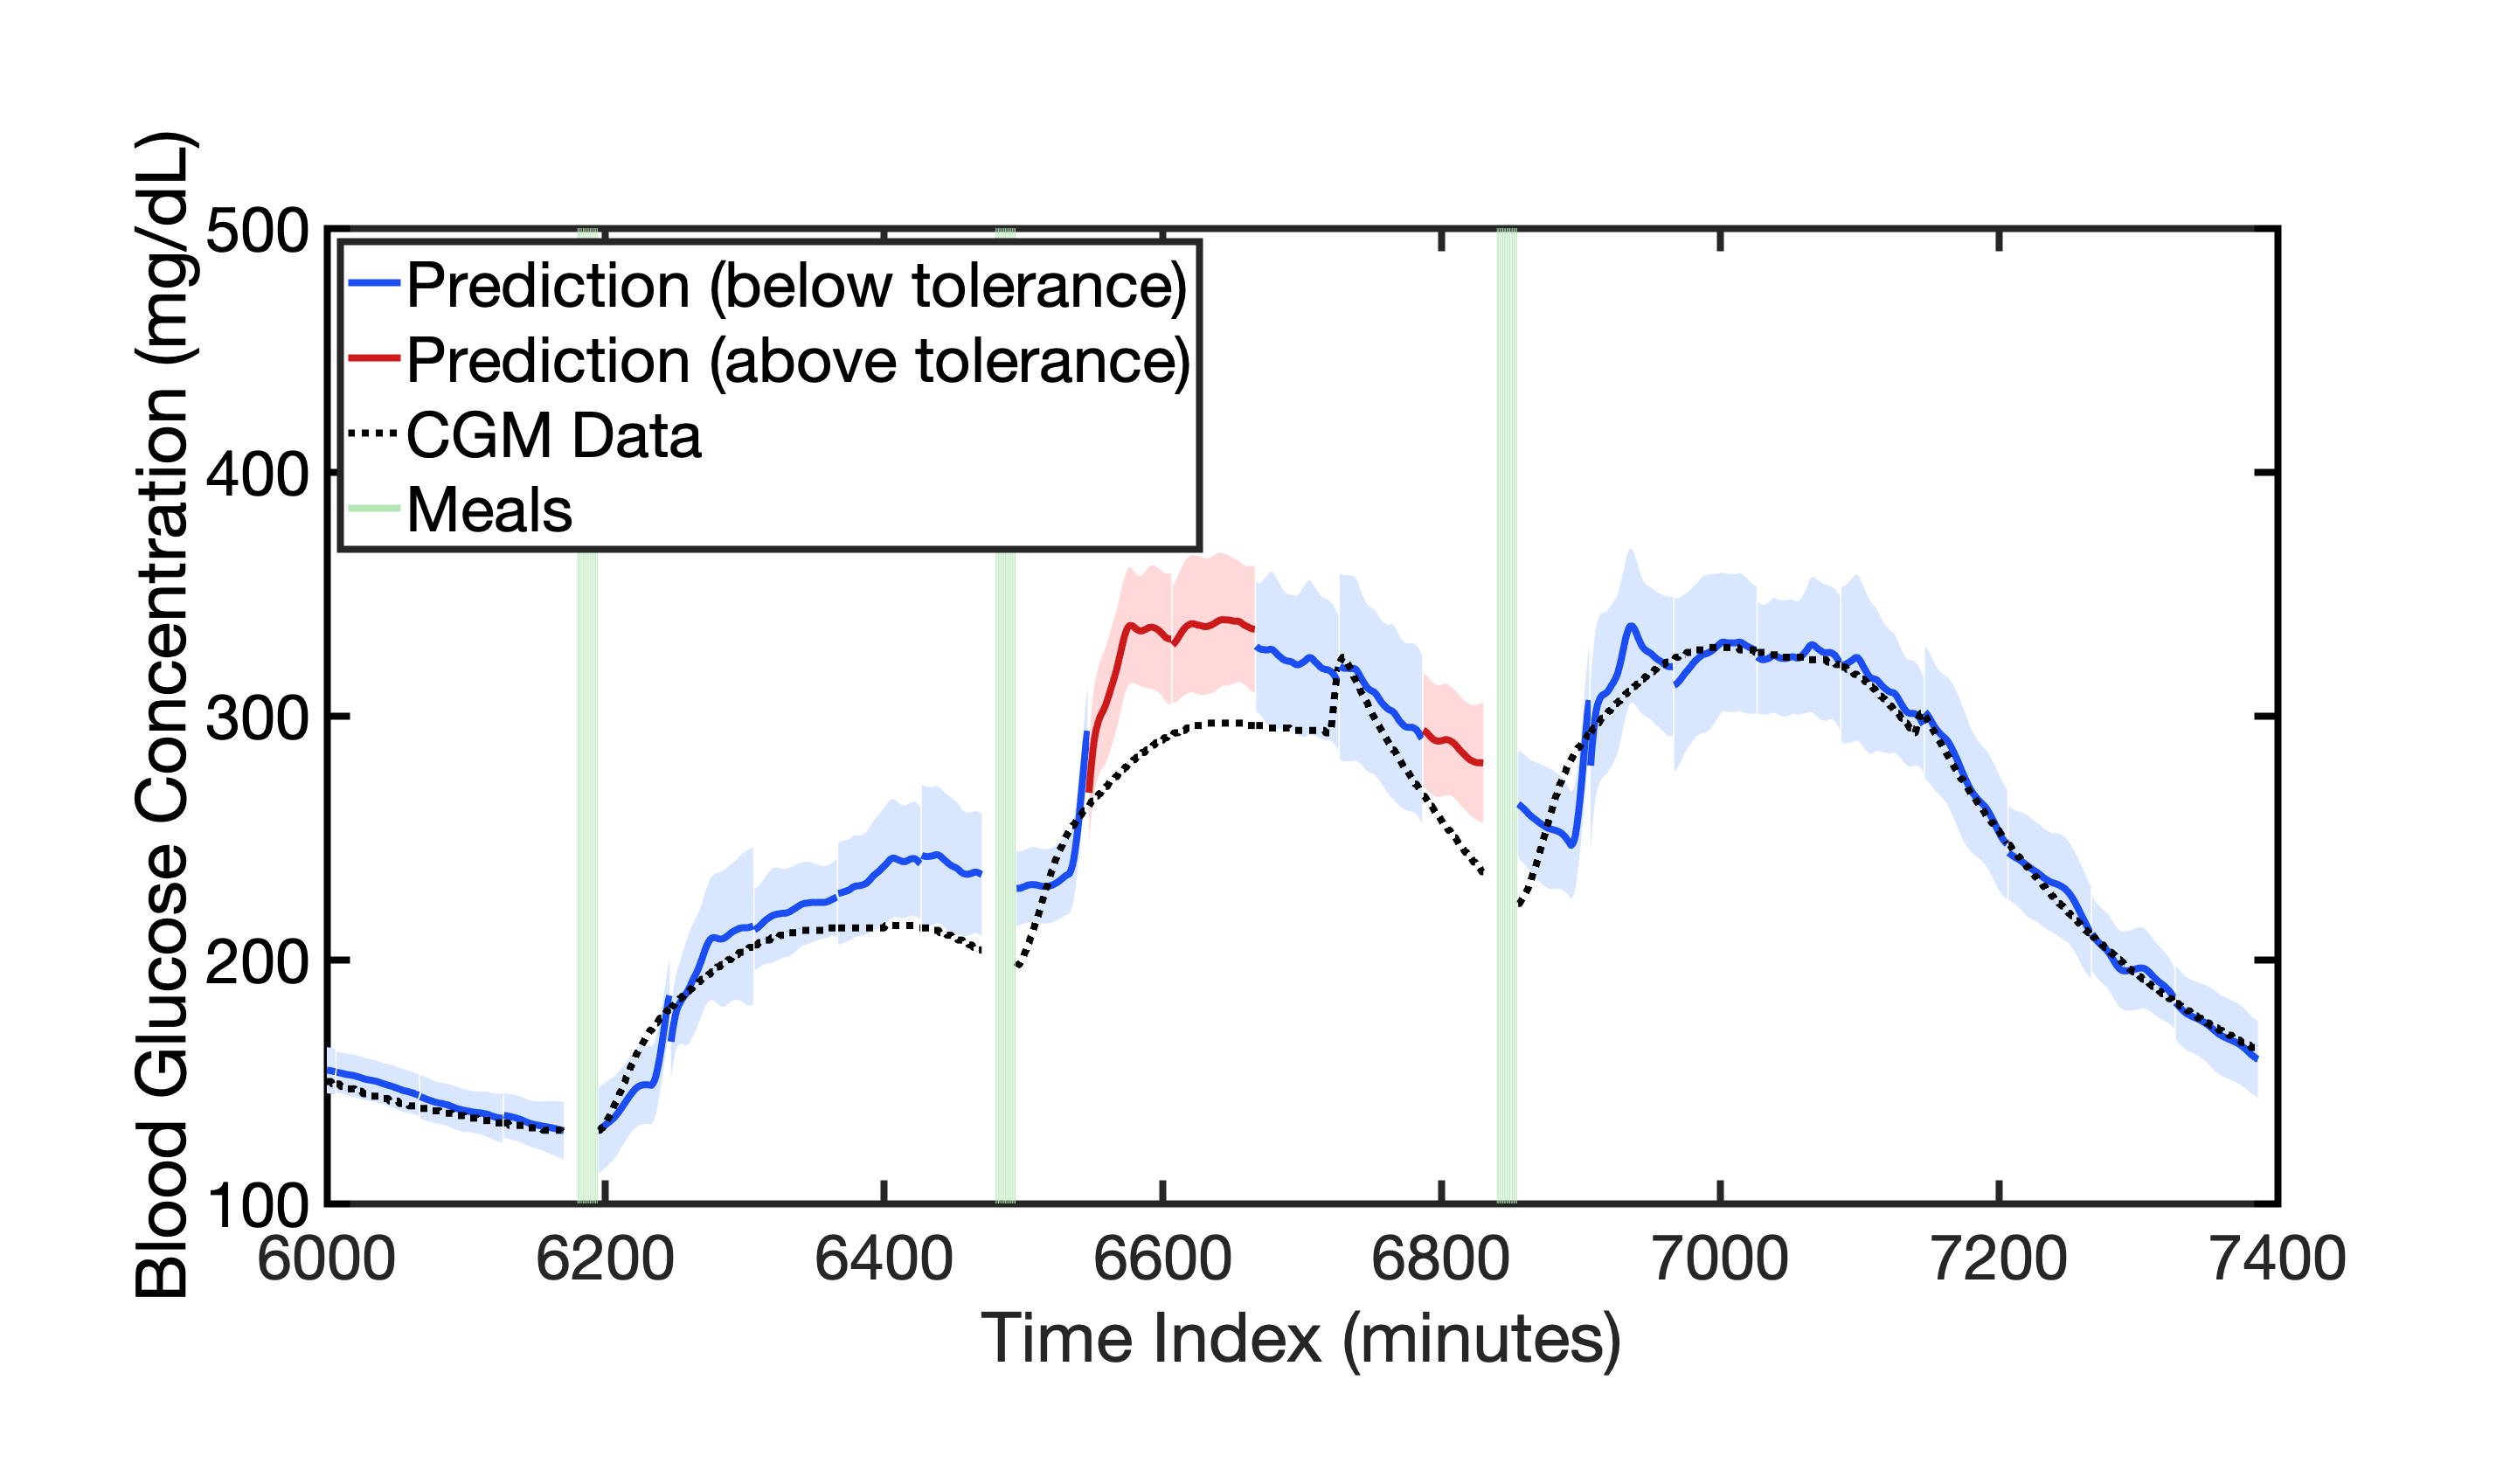
\includegraphics[width=\linewidth]{Figures/Part B/cat1/p3_c1.png}
  \caption*{(c)}
\end{minipage}\hfill
\begin{minipage}[t]{0.48\textwidth}
  \centering
  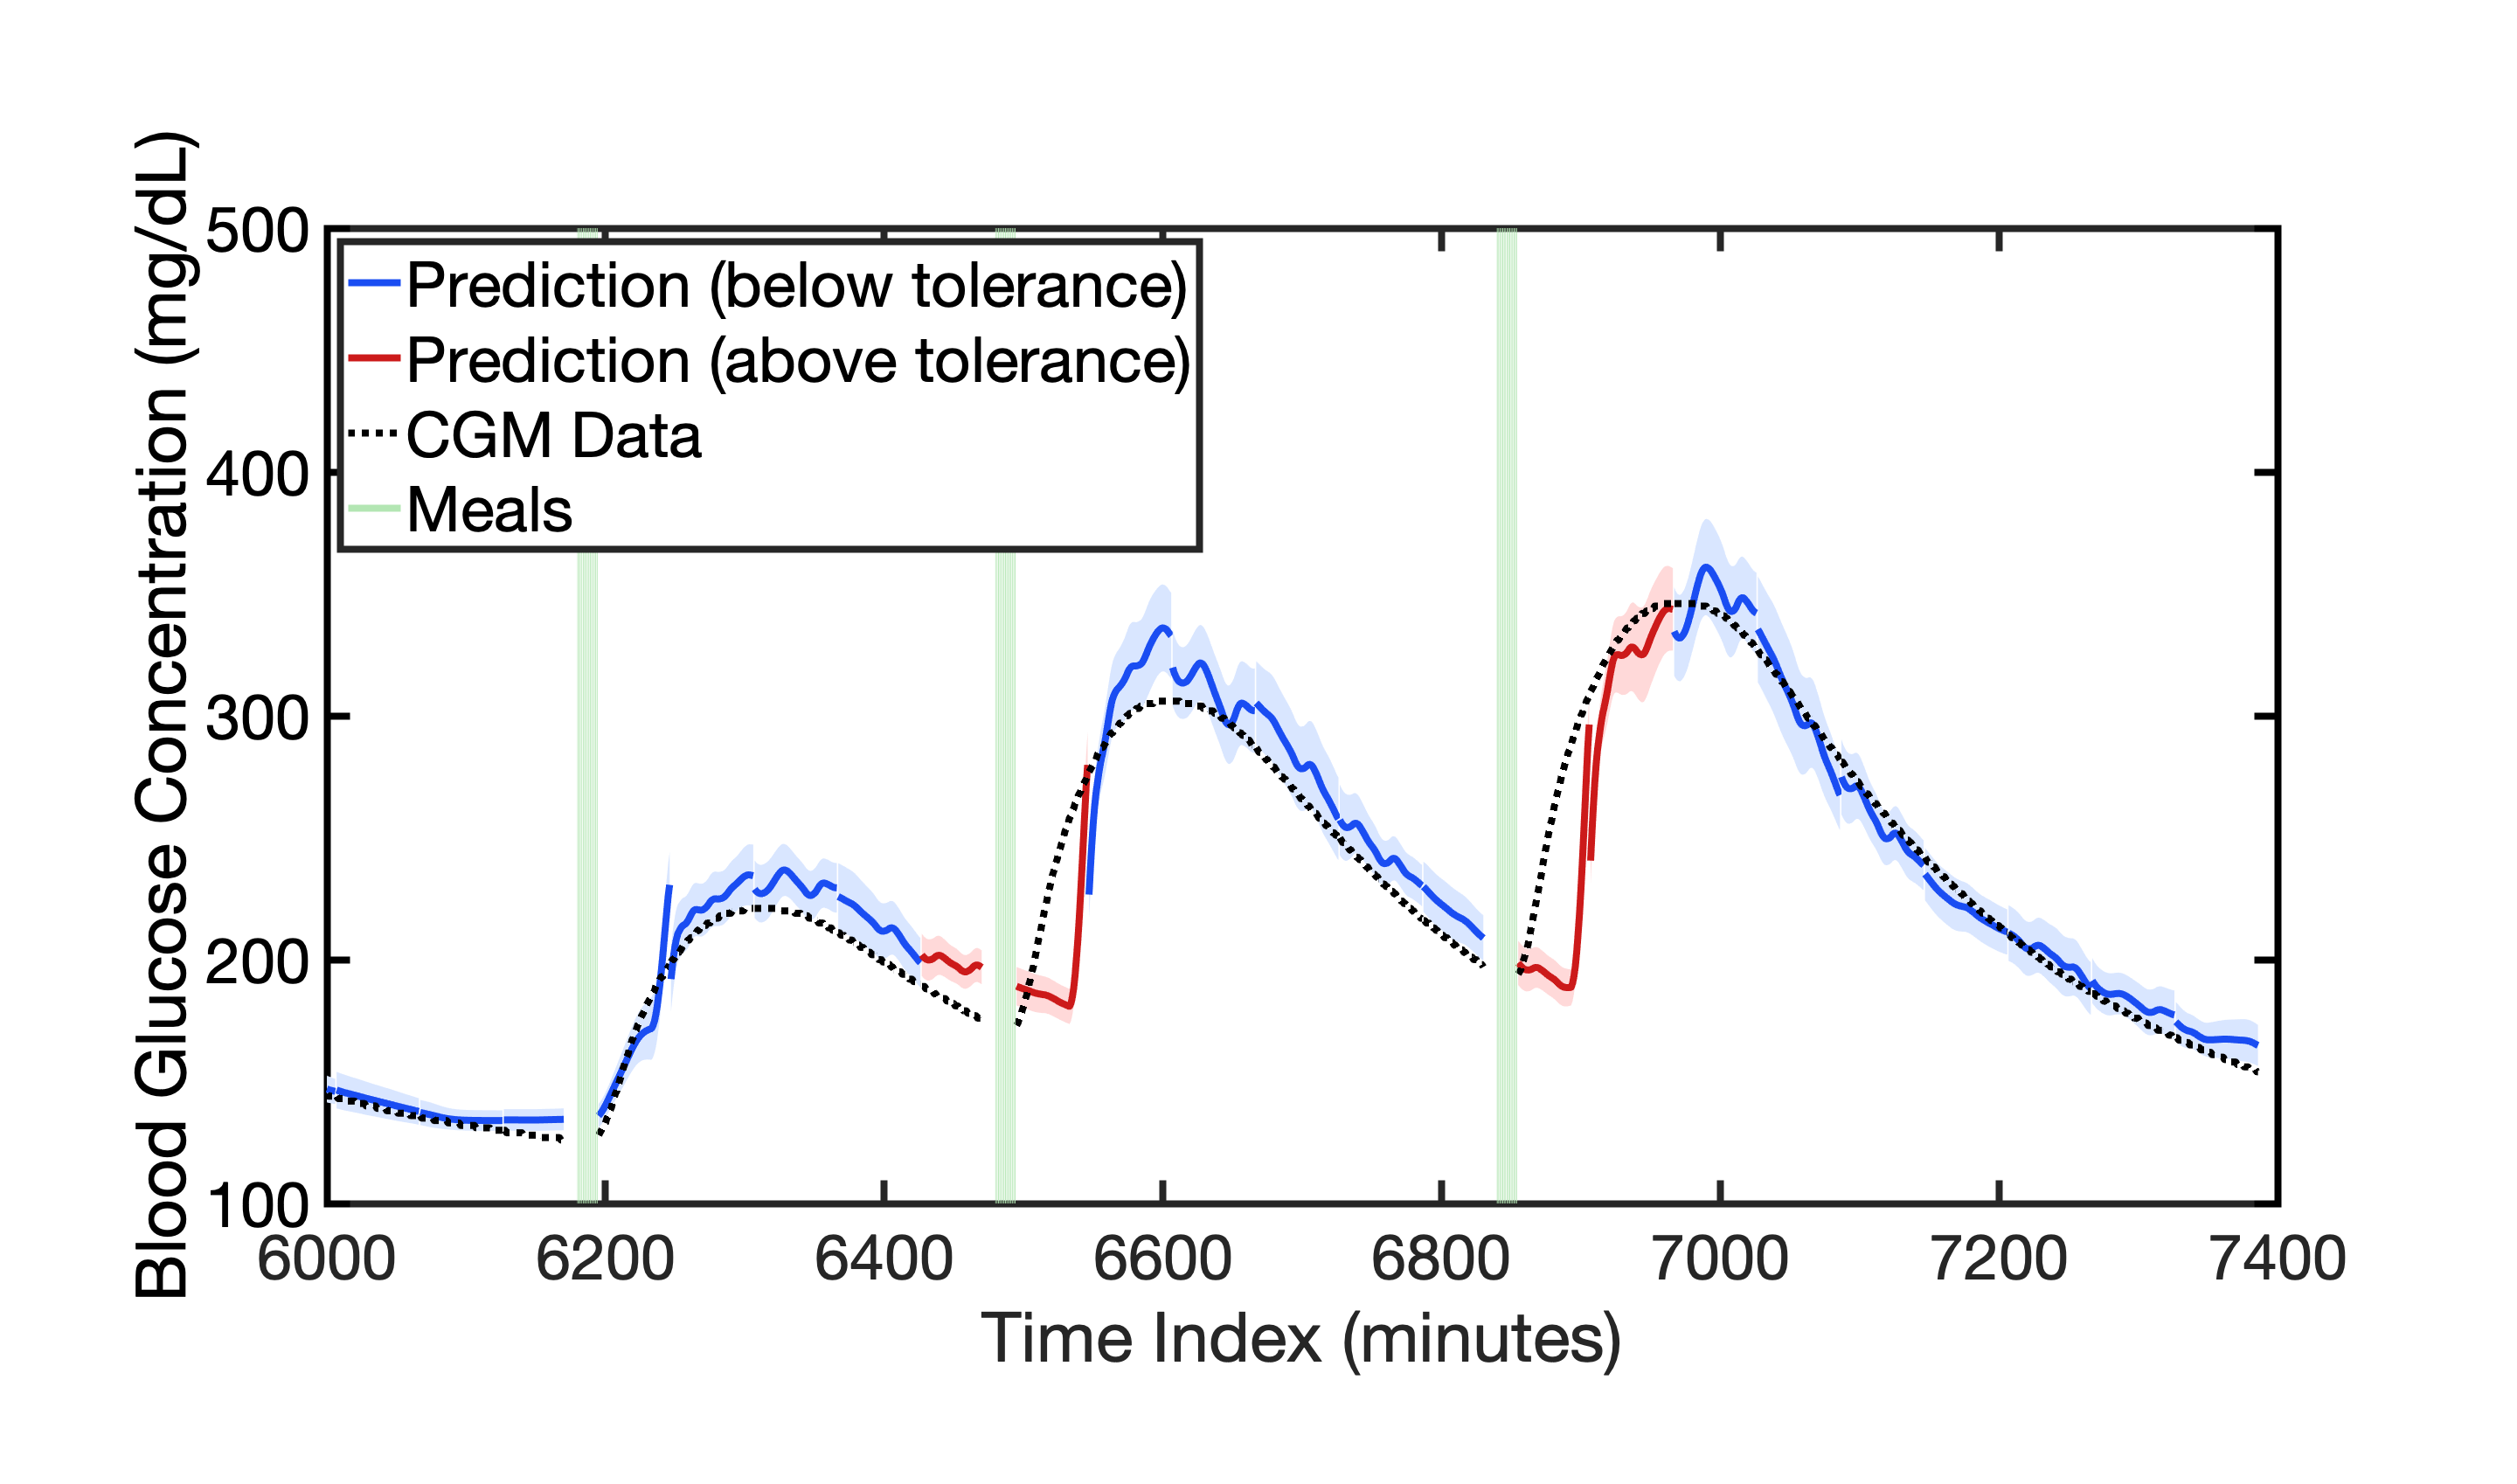
\includegraphics[width=\linewidth]{Figures/Part B/cat1/p9_c1.png}
  \caption*{(d)}
\end{minipage}
\caption{Representative validation for Level~1 architectures on held-out subjects. (a) Patient 2 from fold 3, Architecture: $Level_1Arch_4$, (b) Patient 1 from fold 3, Architecture: $Level_1Arch_4$, (c) Patient 3 from fold 4, Architecture: $Level_1Arch_6$, and Patient 9 from fold 1, Architecture: $Level_1Arch_1$.
Red segments indicate one-hour prediction windows that violates the acceptance criterion $NLPD \leq Tol$.}
\label{fig:cat1-pred}
\end{figure}



\paragraph{Capacity Level~2 ($l=2$)}
Level~2 contains the intermediate-capacity regime ($3\times10^4 - 1\times10^5$ parameters) in which EVIDENT identifies architectures that are both plausible and validation-acceptable. 
%-- Level 2: plausibility/sigma-noise
Figure \ref{fig:cat2_plausibility_sigma} summarizes, for each held-out validation fold, the variation of posterior plausibility $\rho$ and the corresponding MAP estimate of $\sigma_{\text{noise}}$ across the candidate architectures in this level. It is observed that a small subset of architectures receives substantial posterior model plausibility, while the most plausible architecture varies across folds, reflecting the inter-patient heterogeneity of the population-based training data in Figure \ref{fig:uva}. While most subjects exhibit comparable glucose ranges and excursion patterns, Patient 7 and Patient 5 display substantially larger amplitudes, which changes the temporal structure seen during training. As a result, EVIDENT favors different architectures across folds. Nevertheless, $Level_2Arch_4$ with 43268 parameters, which consists of 5 temporal blocks with dilation base ($b=3$), kernel size ($f=9$), and encoder channels ($[2,4,8,16,32]$), emerges as a competitive architecture in three validation folds. This architecture achieves a one-day receptive field through gradual dilation growth across depth, while retaining sufficient local temporal resolution to capture meal-driven glucose excursions.
The $\sigma_{{\rm noise}_{MAP}}$ trends provide a diagnostic such that low-plausibility architectures require inflated noise levels, indicating that unresolved temporal structure is absorbed as noise, whereas competitive models achieve high plausibility without such inflation.


\begin{figure}[!ht]
\centering
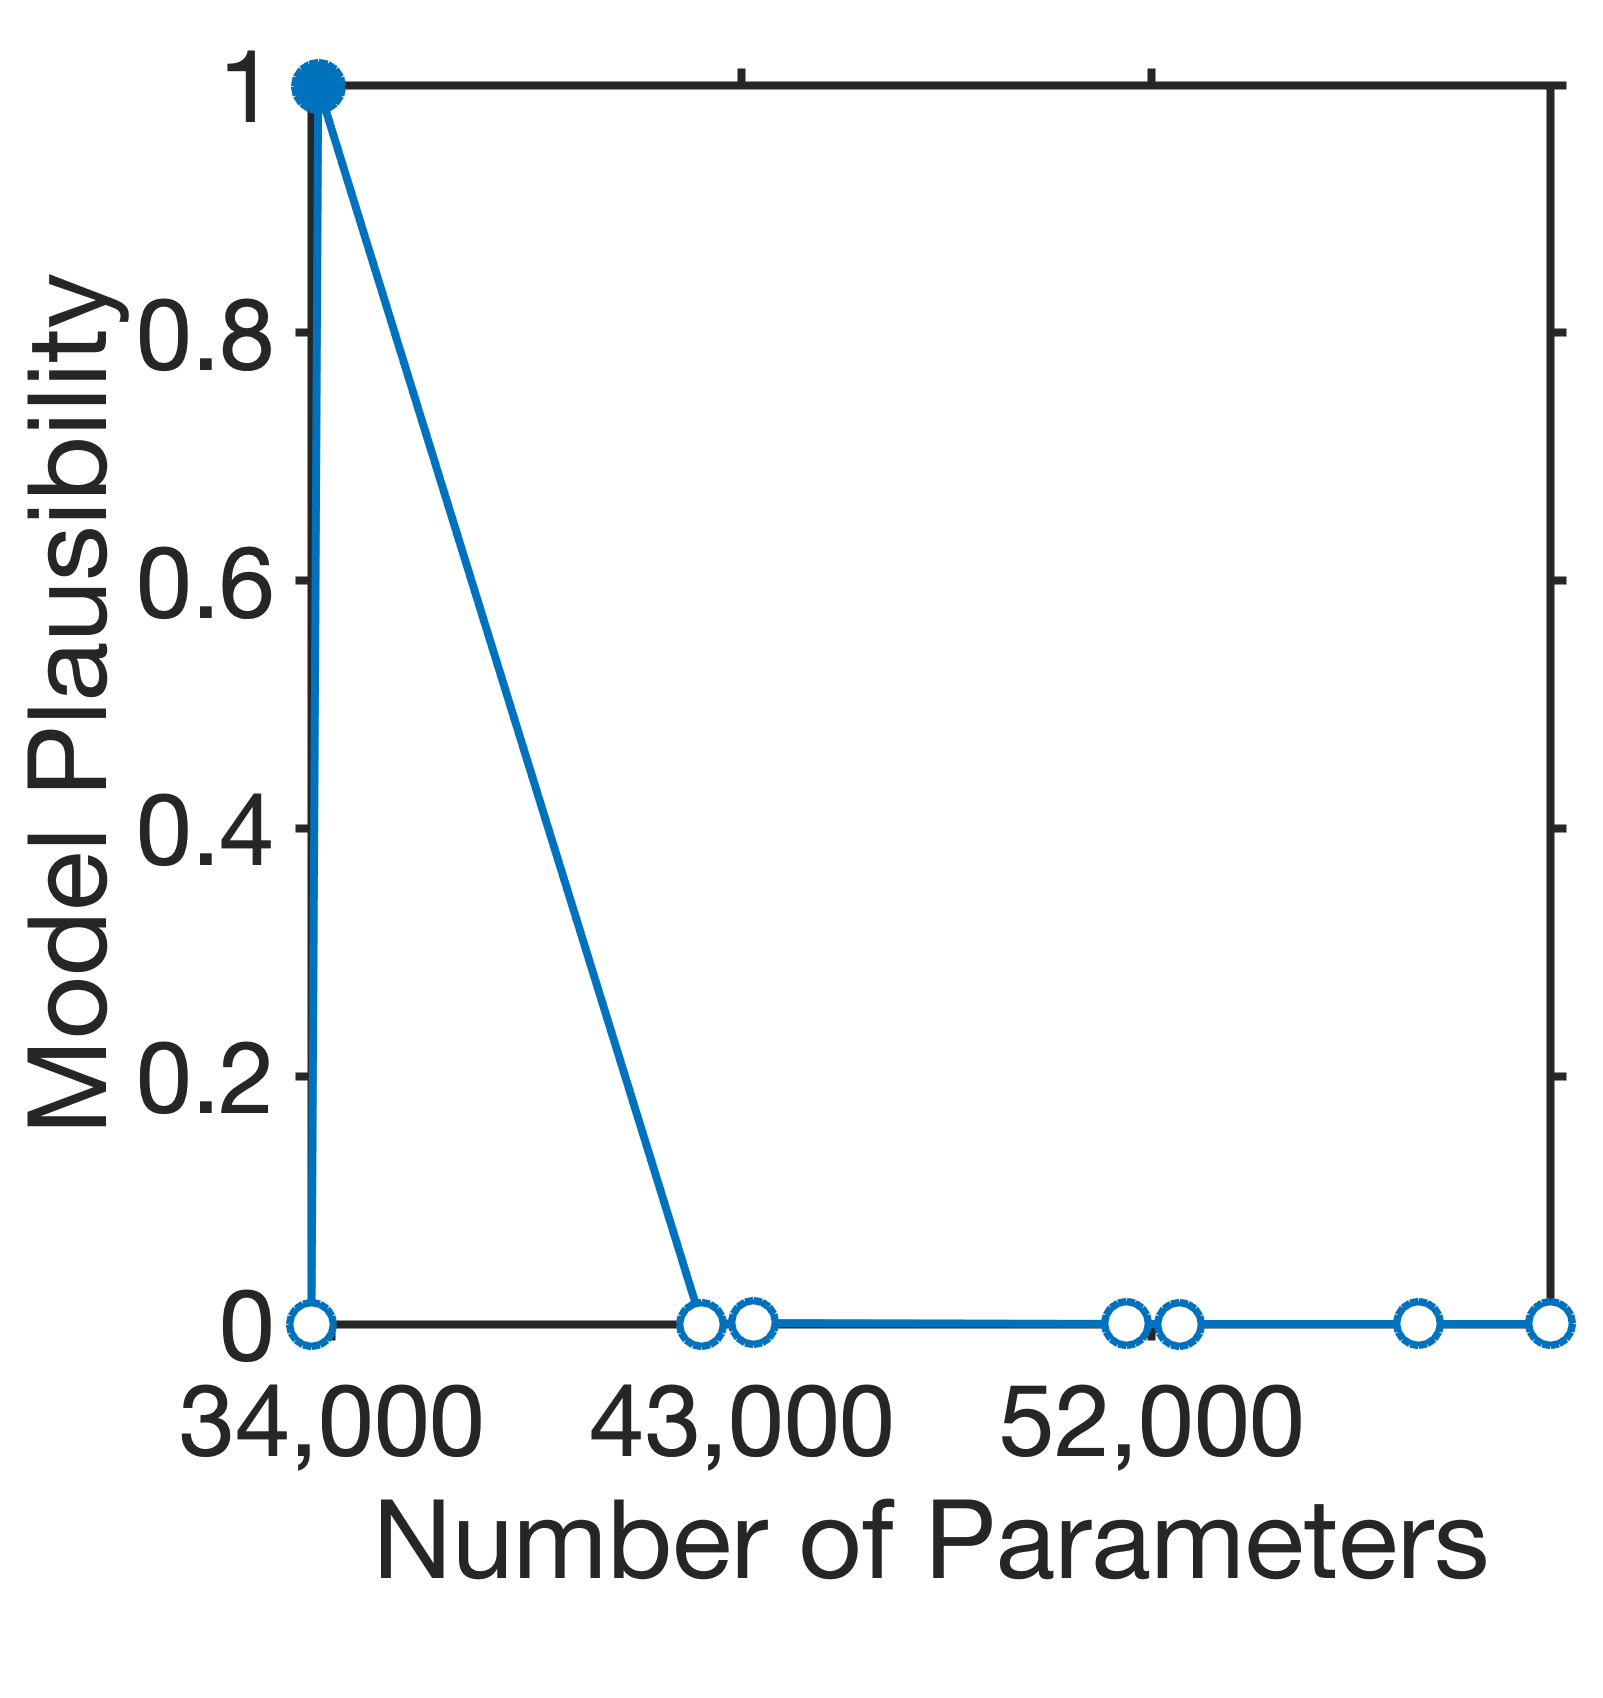
\includegraphics[width=0.19\textwidth]{Figures/Part B/cat2/fold1.png}\hfill
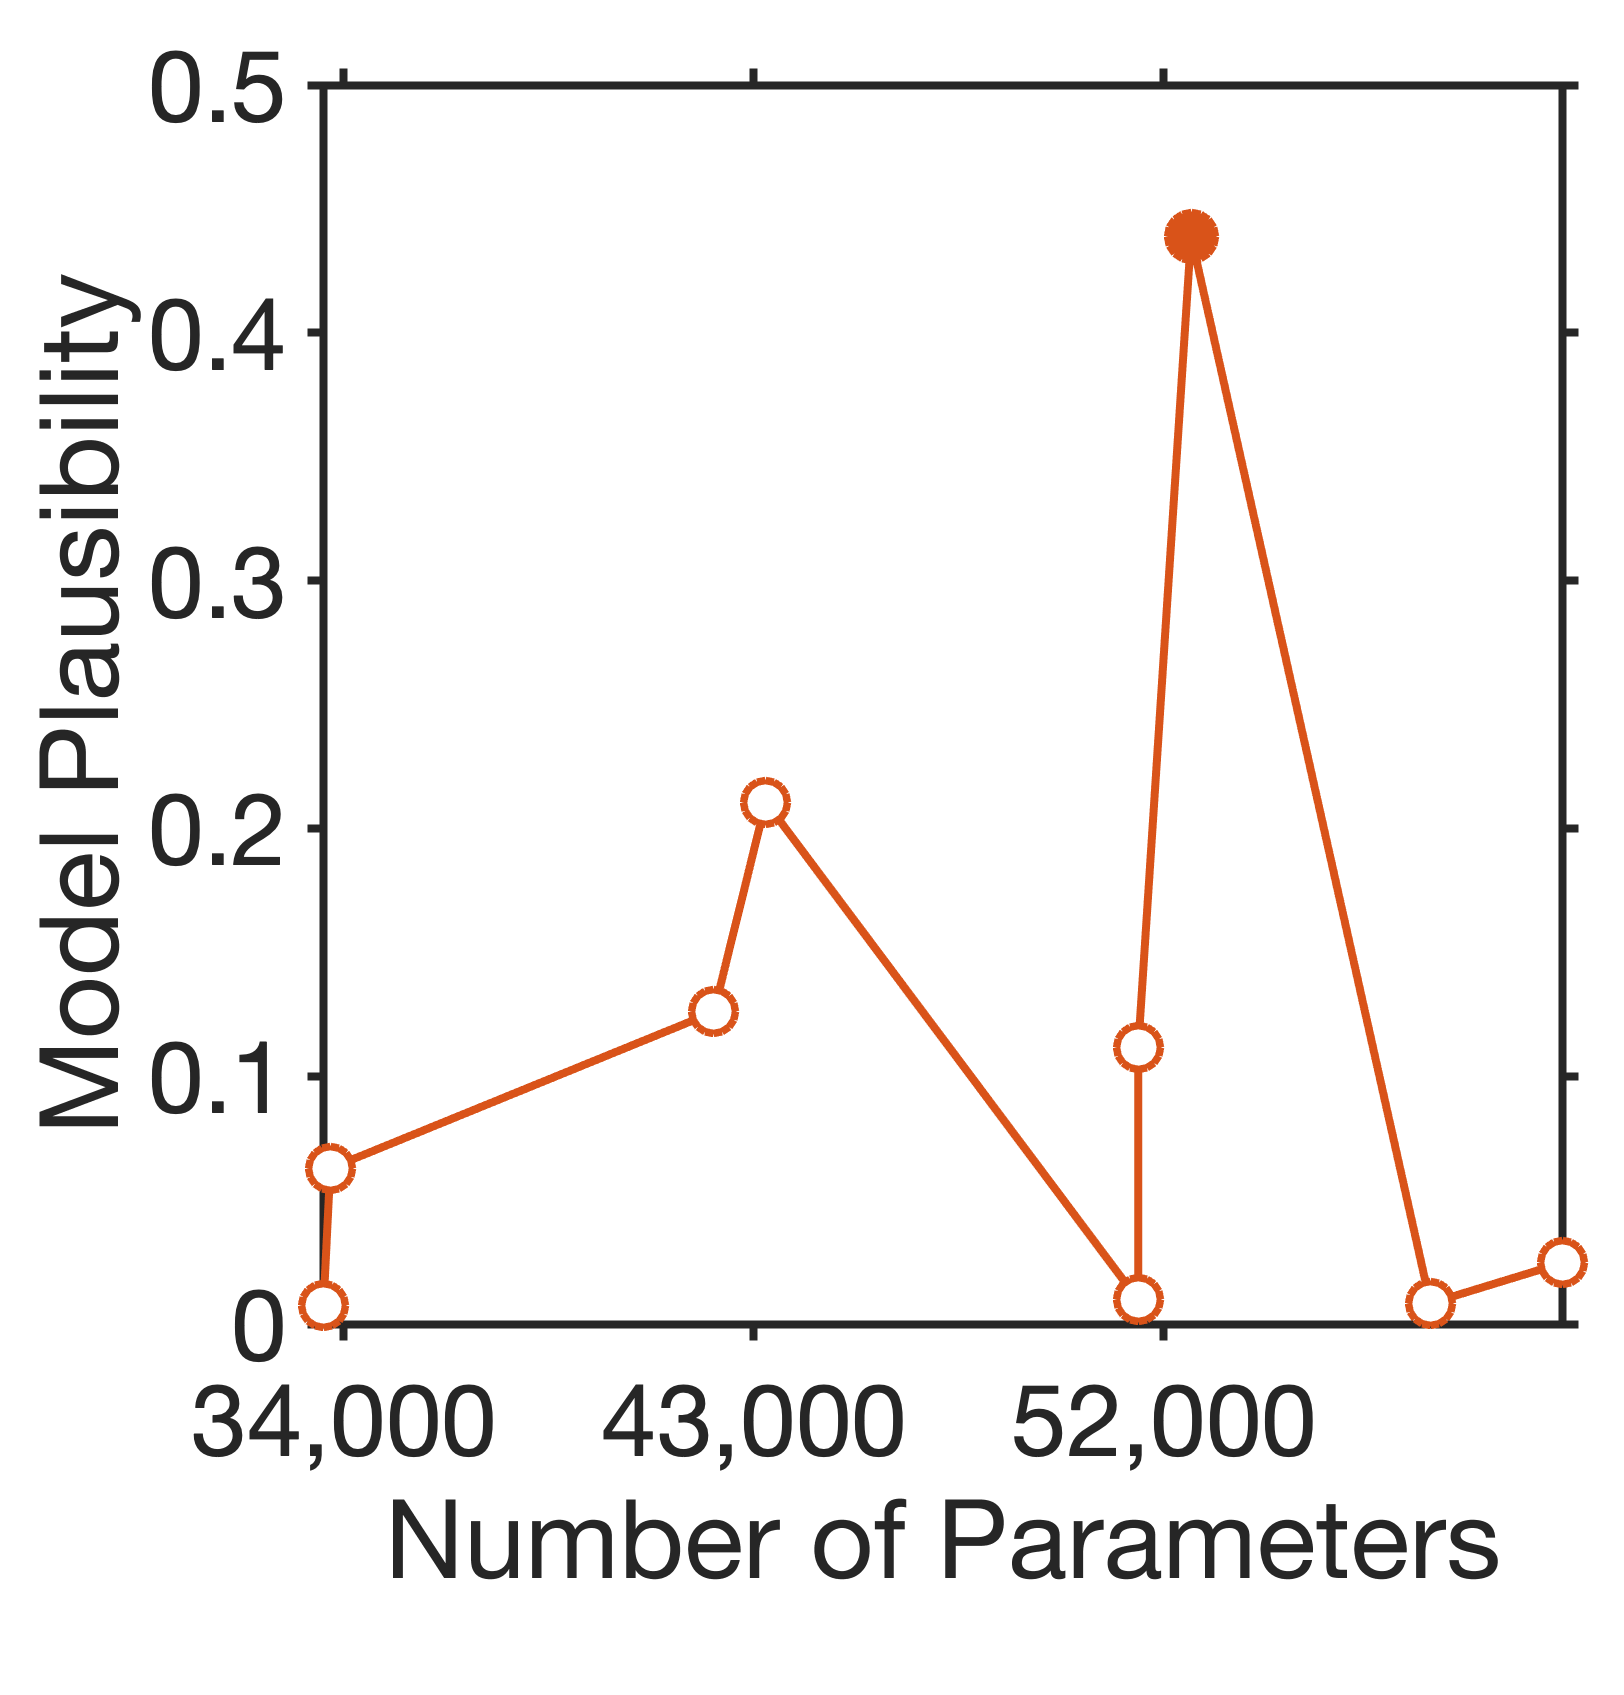
\includegraphics[width=0.19\textwidth]{Figures/Part B/cat2/fold2.png}\hfill
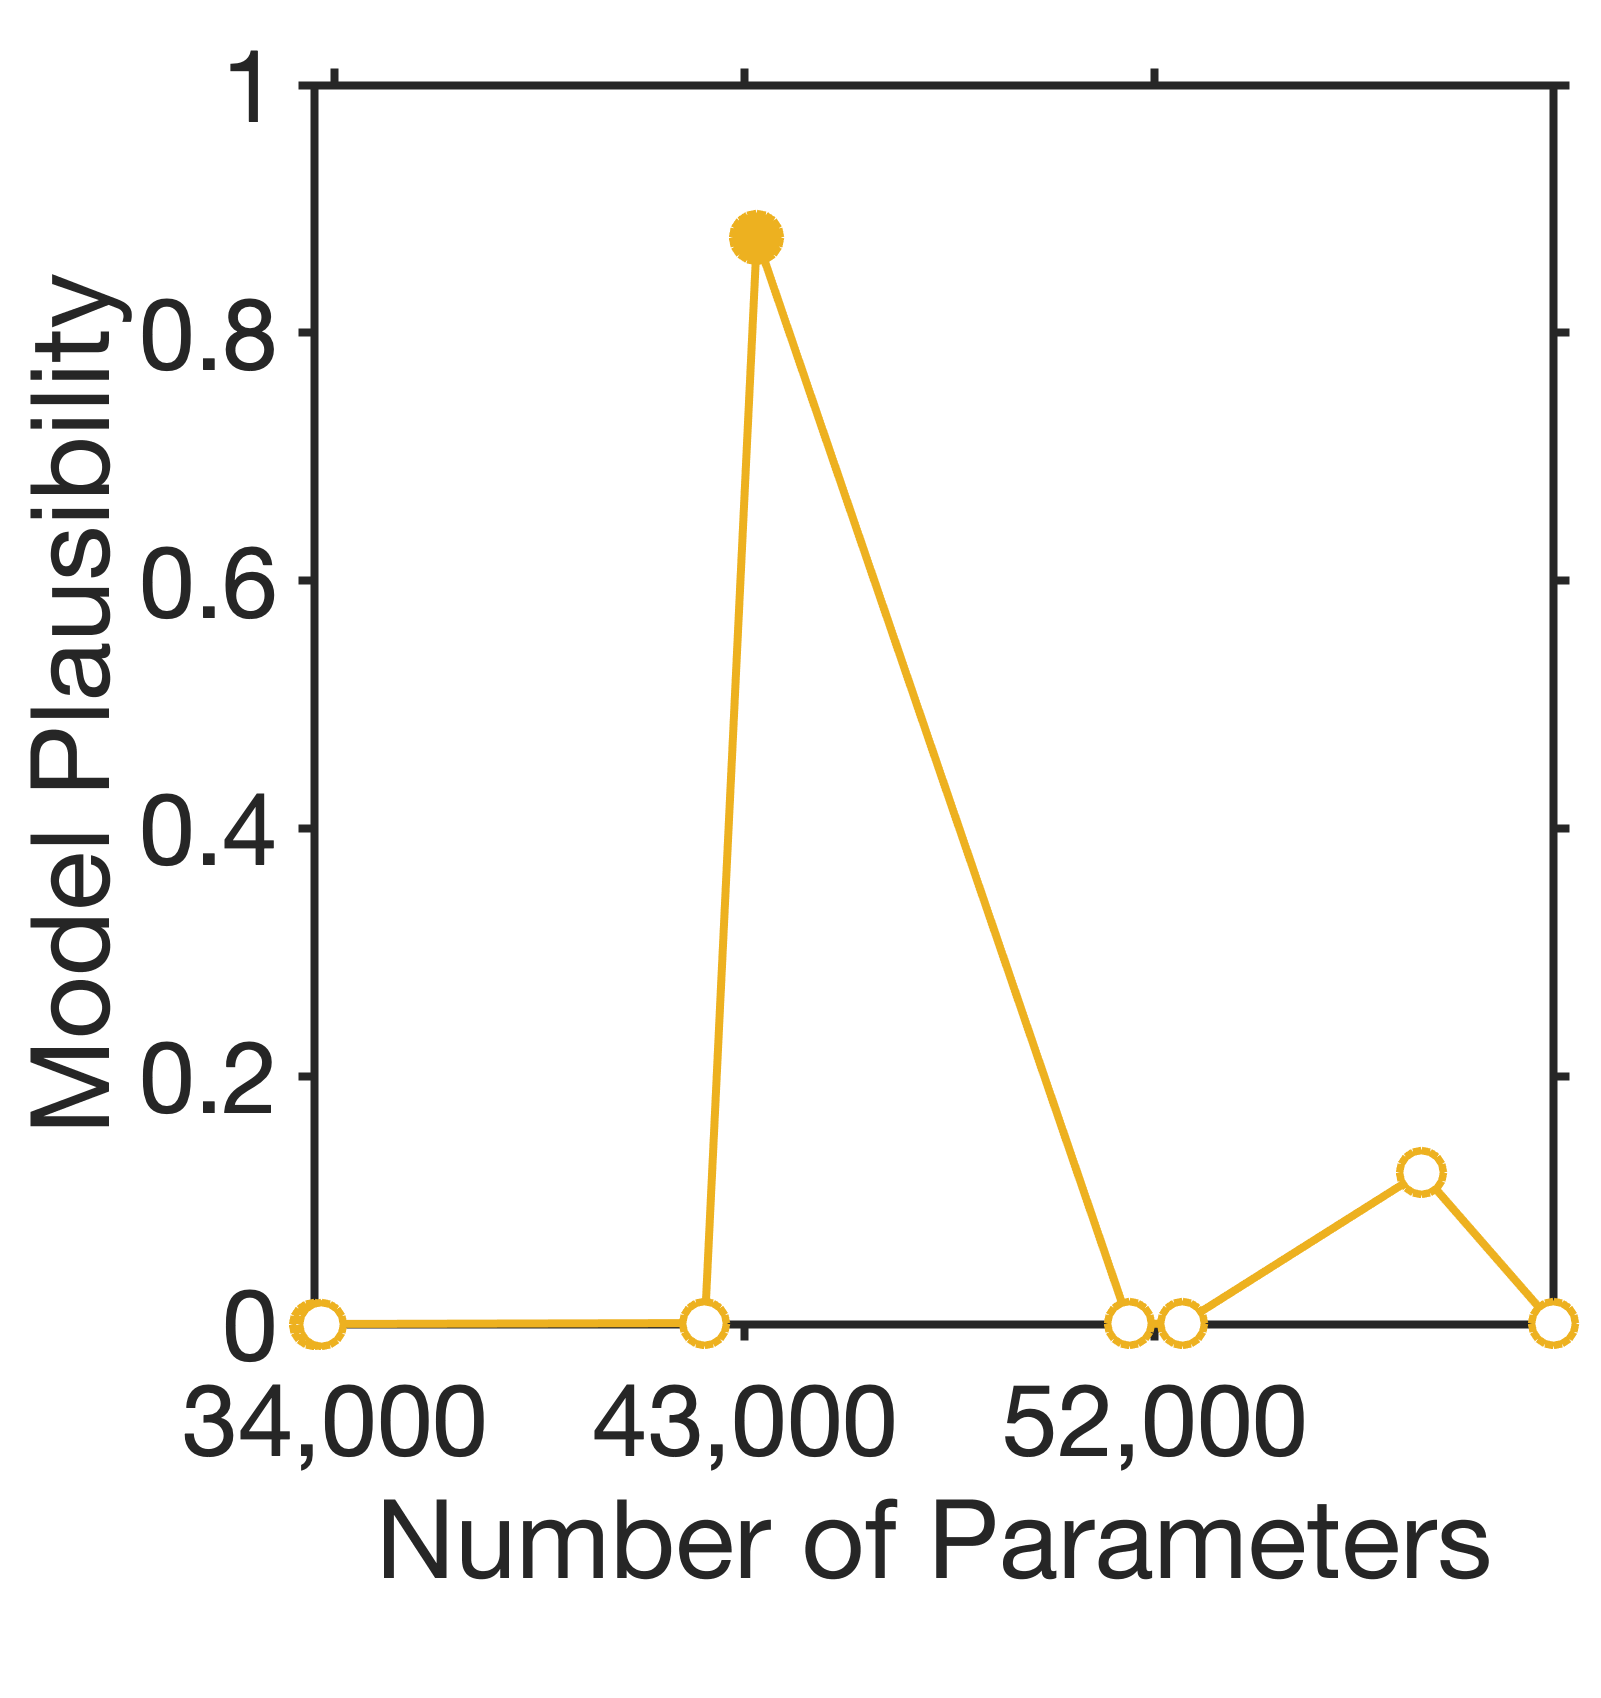
\includegraphics[width=0.19\textwidth]{Figures/Part B/cat2/fold3.png}\hfill
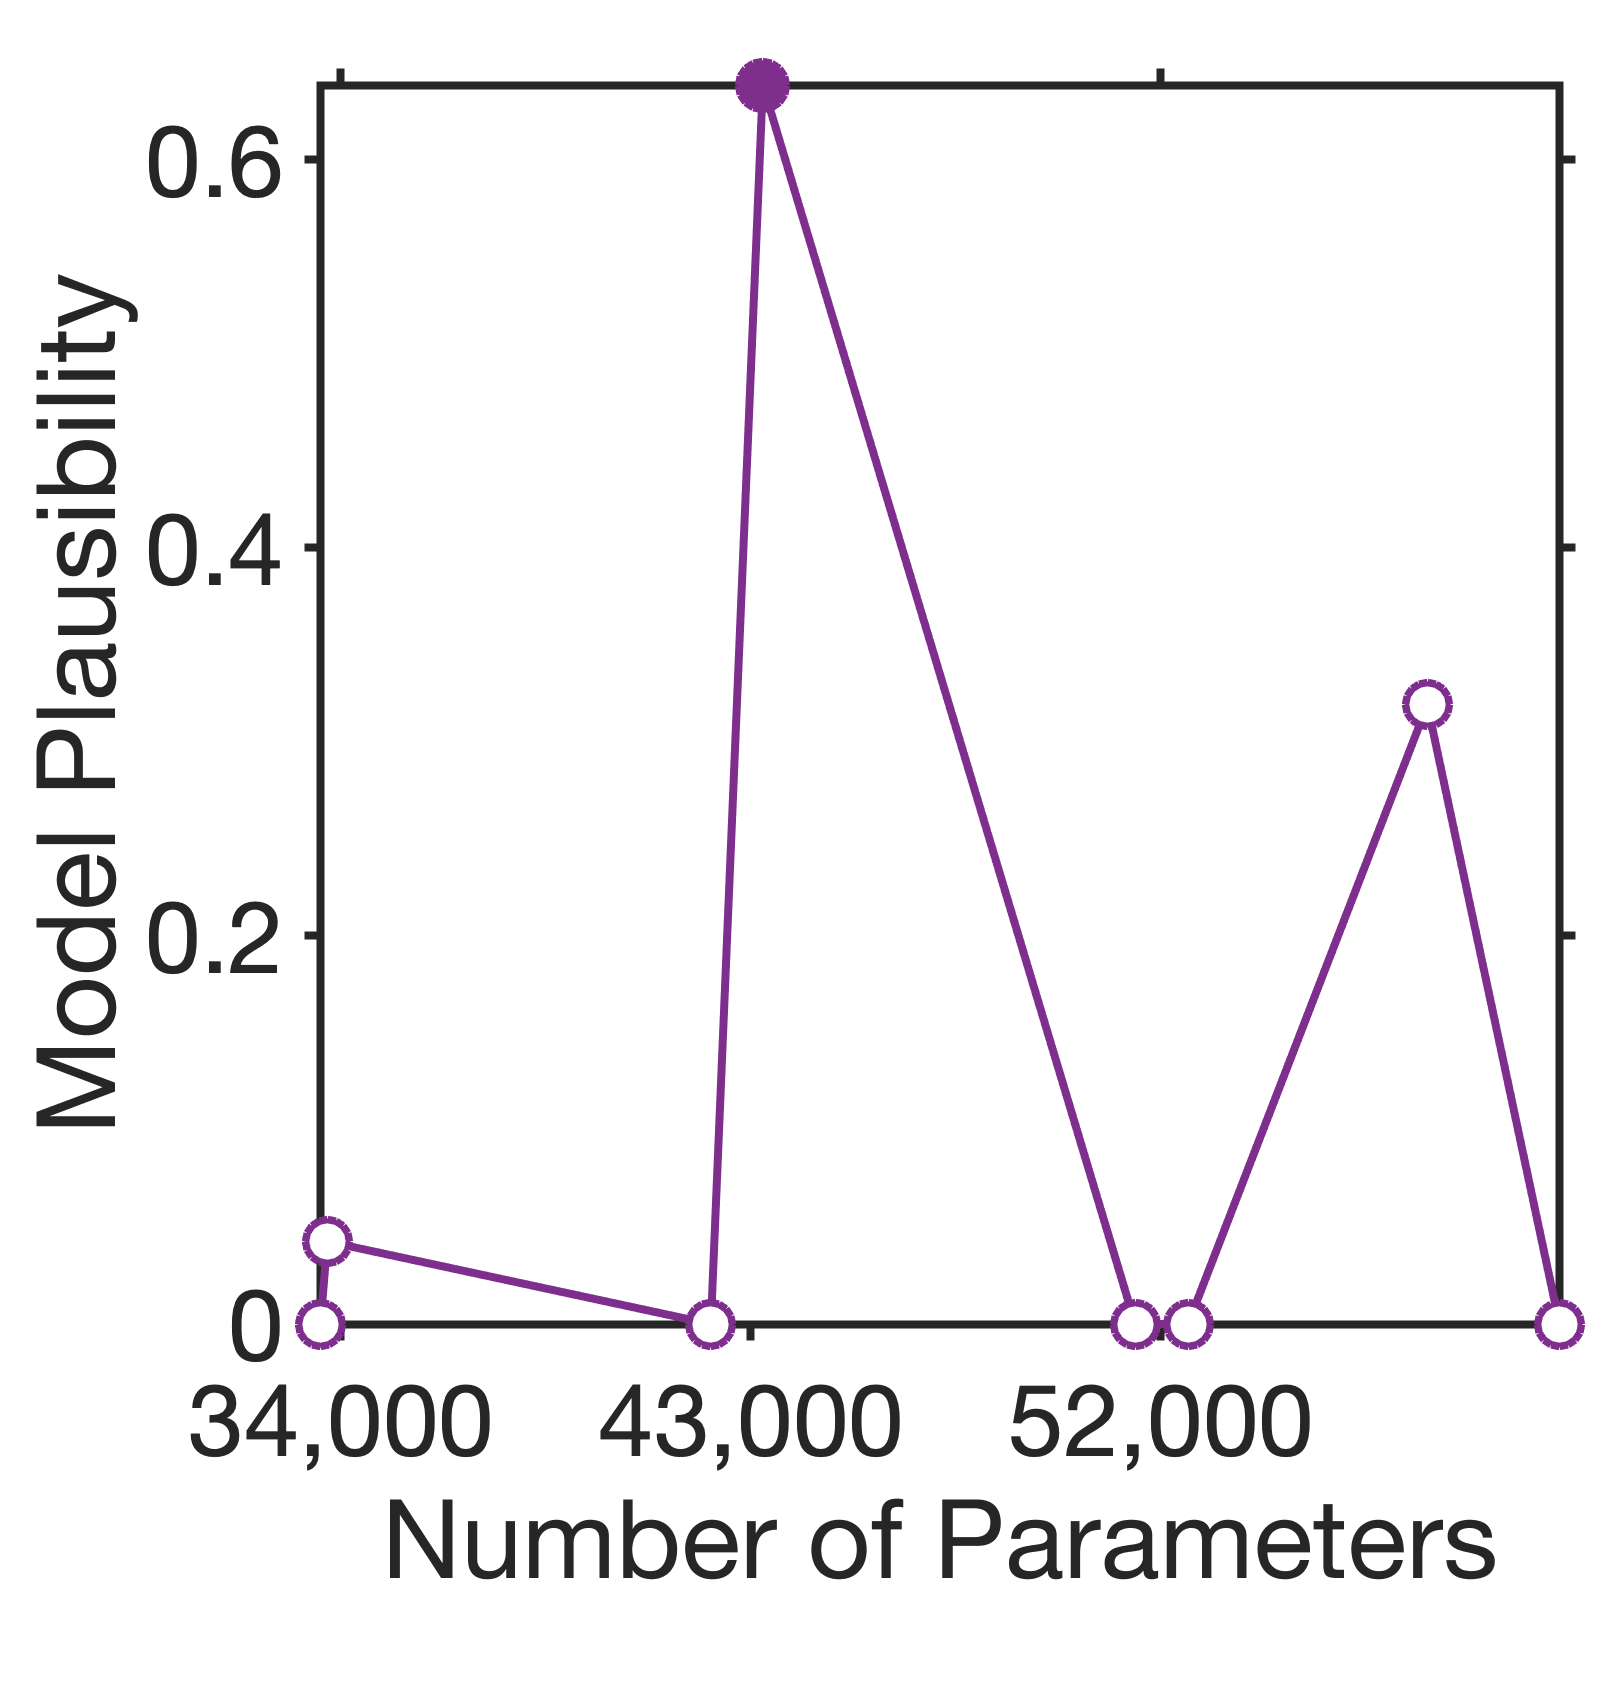
\includegraphics[width=0.19\textwidth]{Figures/Part B/cat2/fold4.png}\hfill
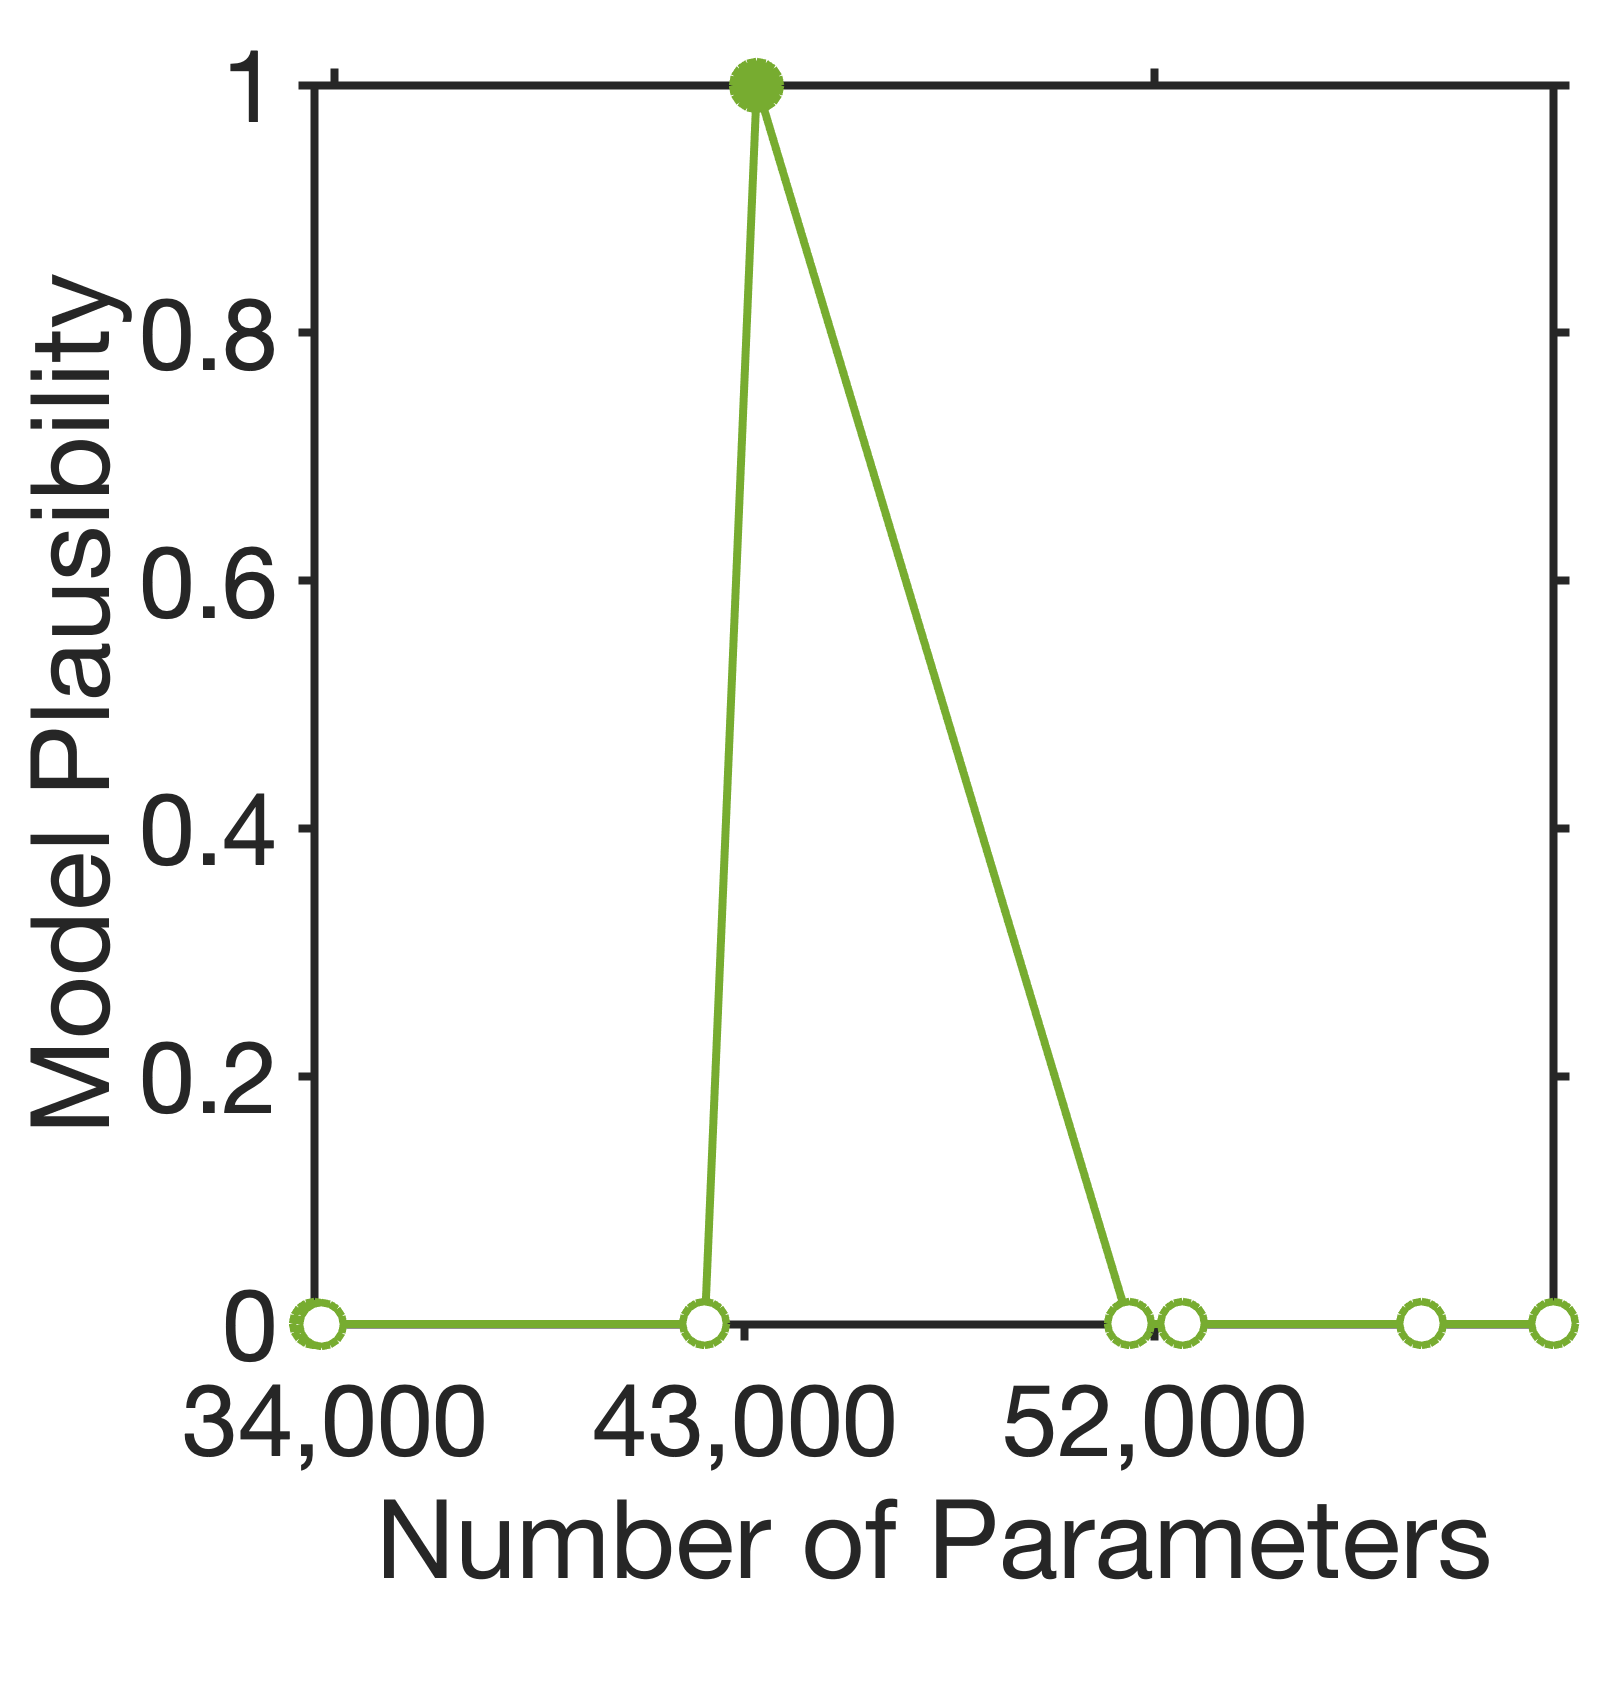
\includegraphics[width=0.19\textwidth]{Figures/Part B/cat2/fold5.png}
\\ (a) \\
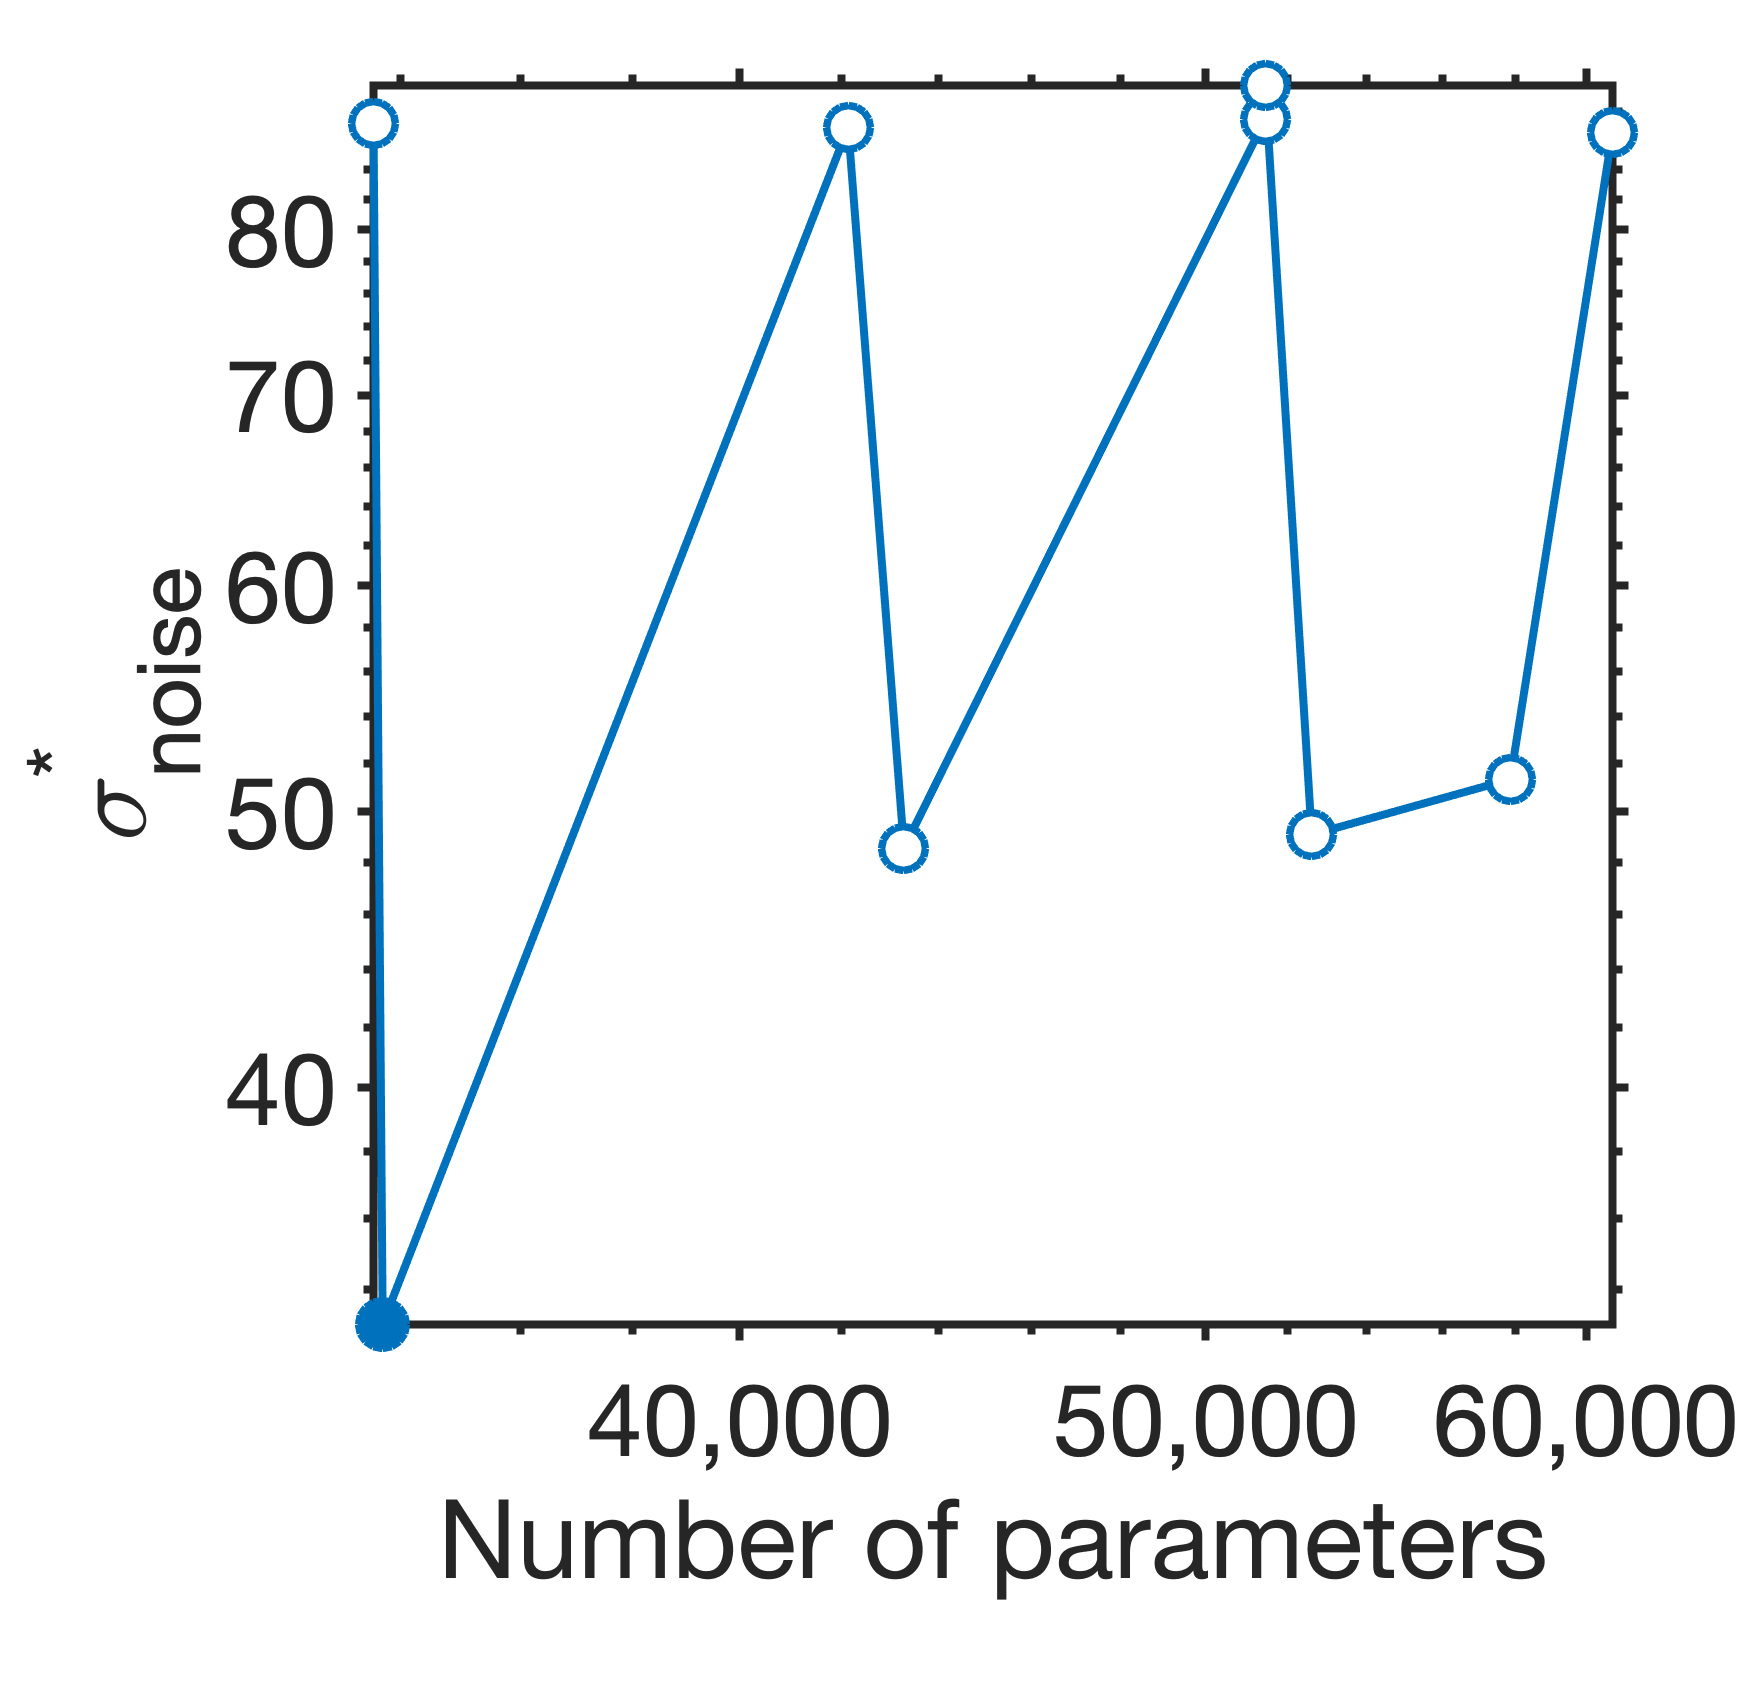
\includegraphics[width=0.19\textwidth]{Figures/Part B/cat2/fold1_noise.png}\hfill
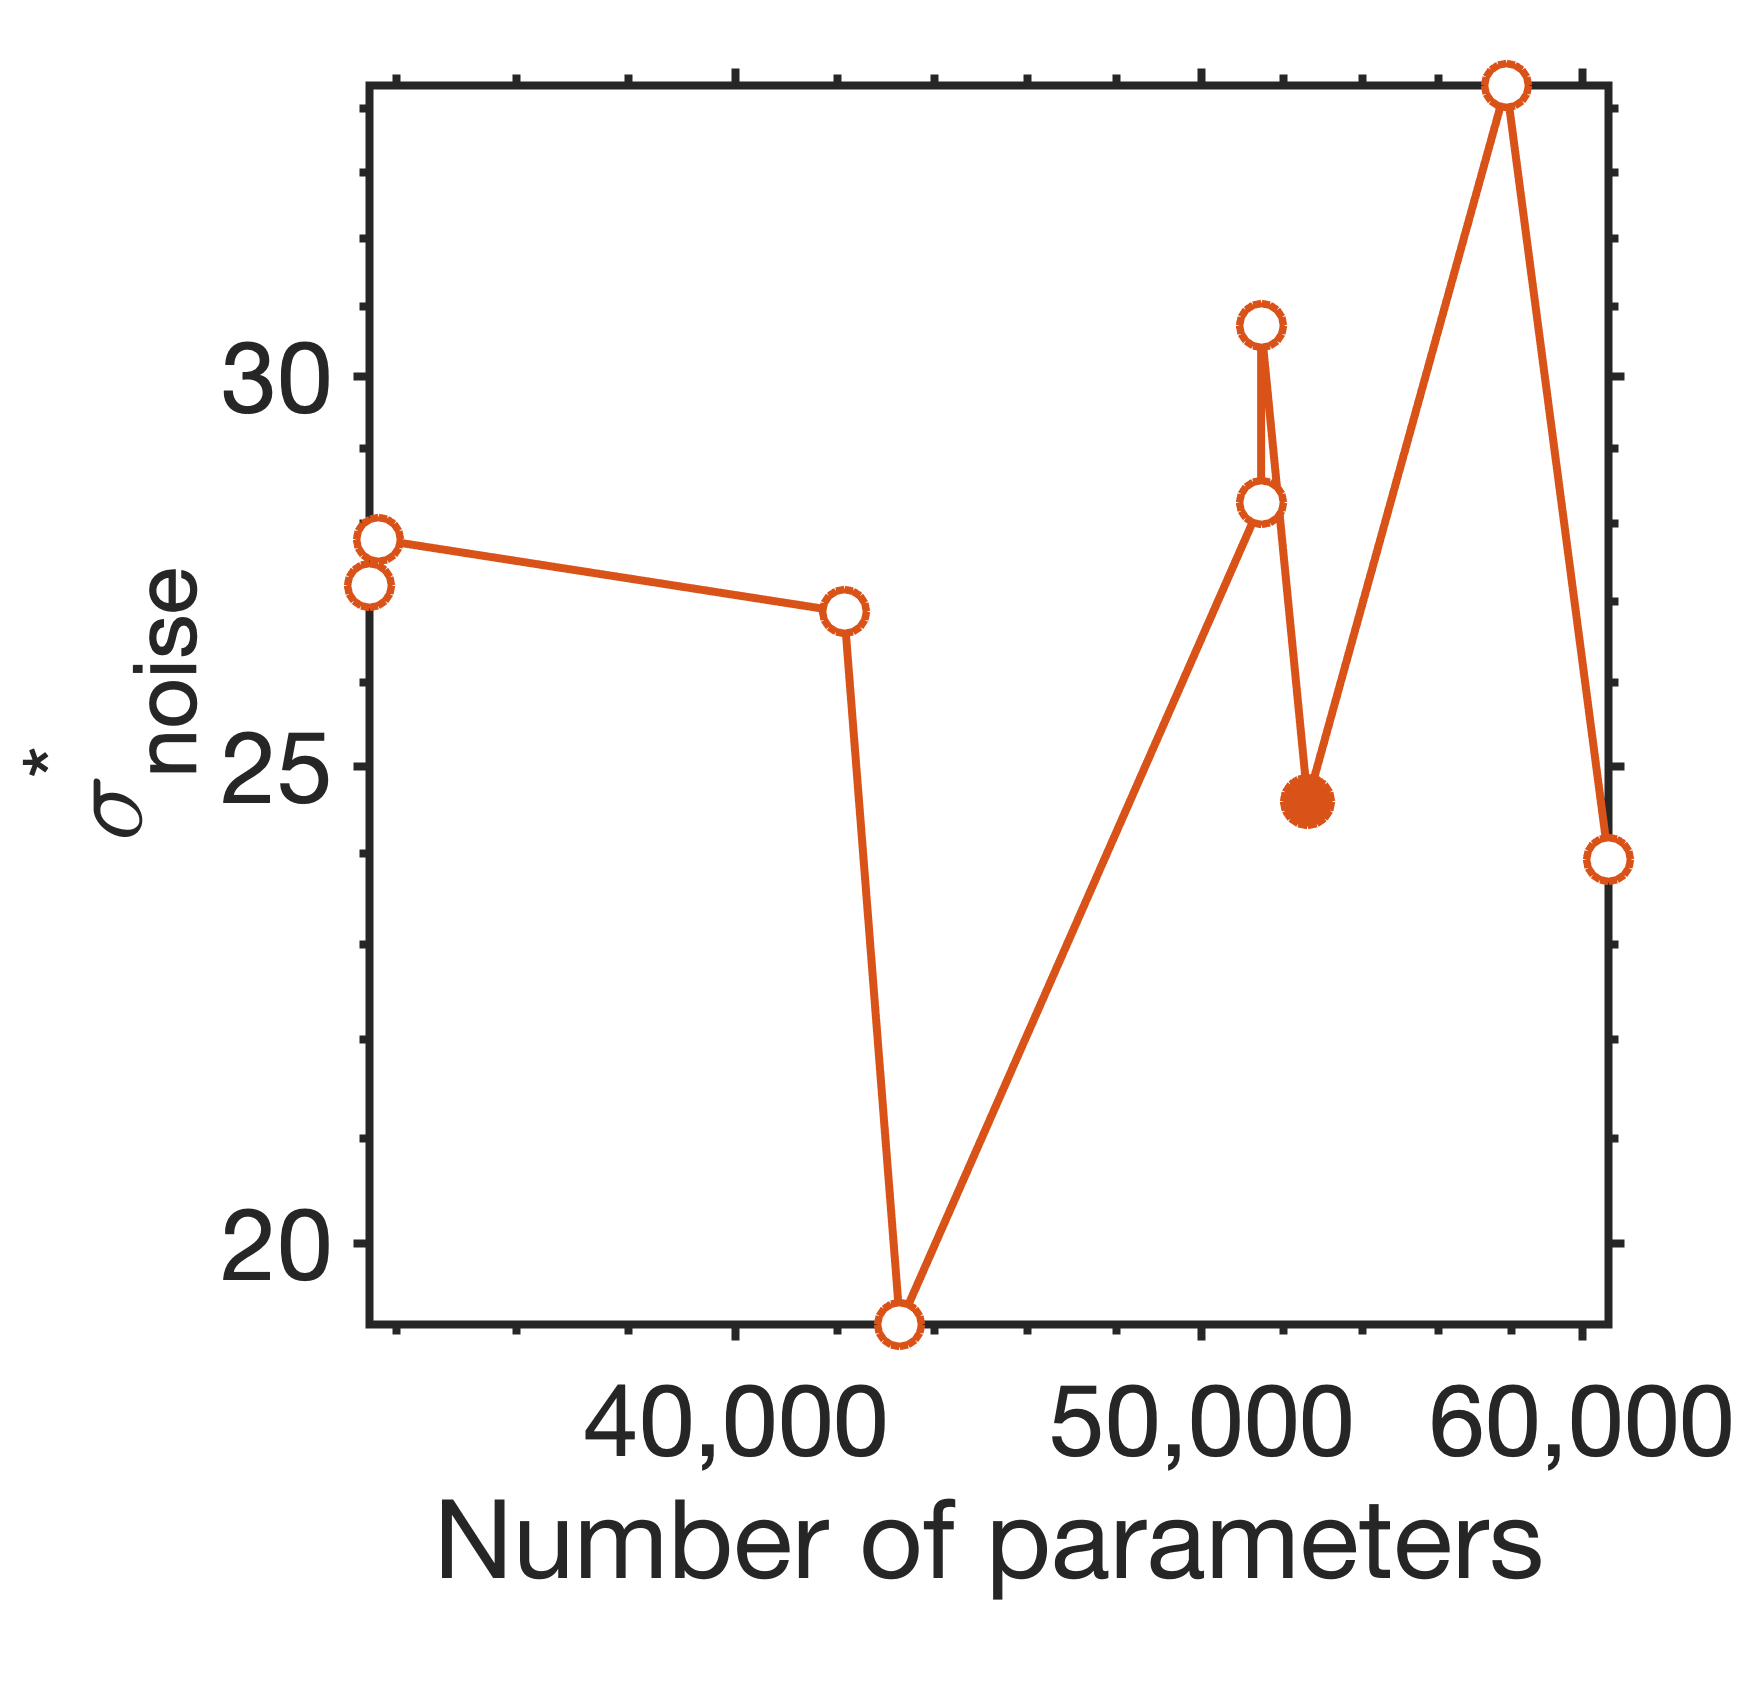
\includegraphics[width=0.19\textwidth]{Figures/Part B/cat2/fold2_noise.png}\hfill
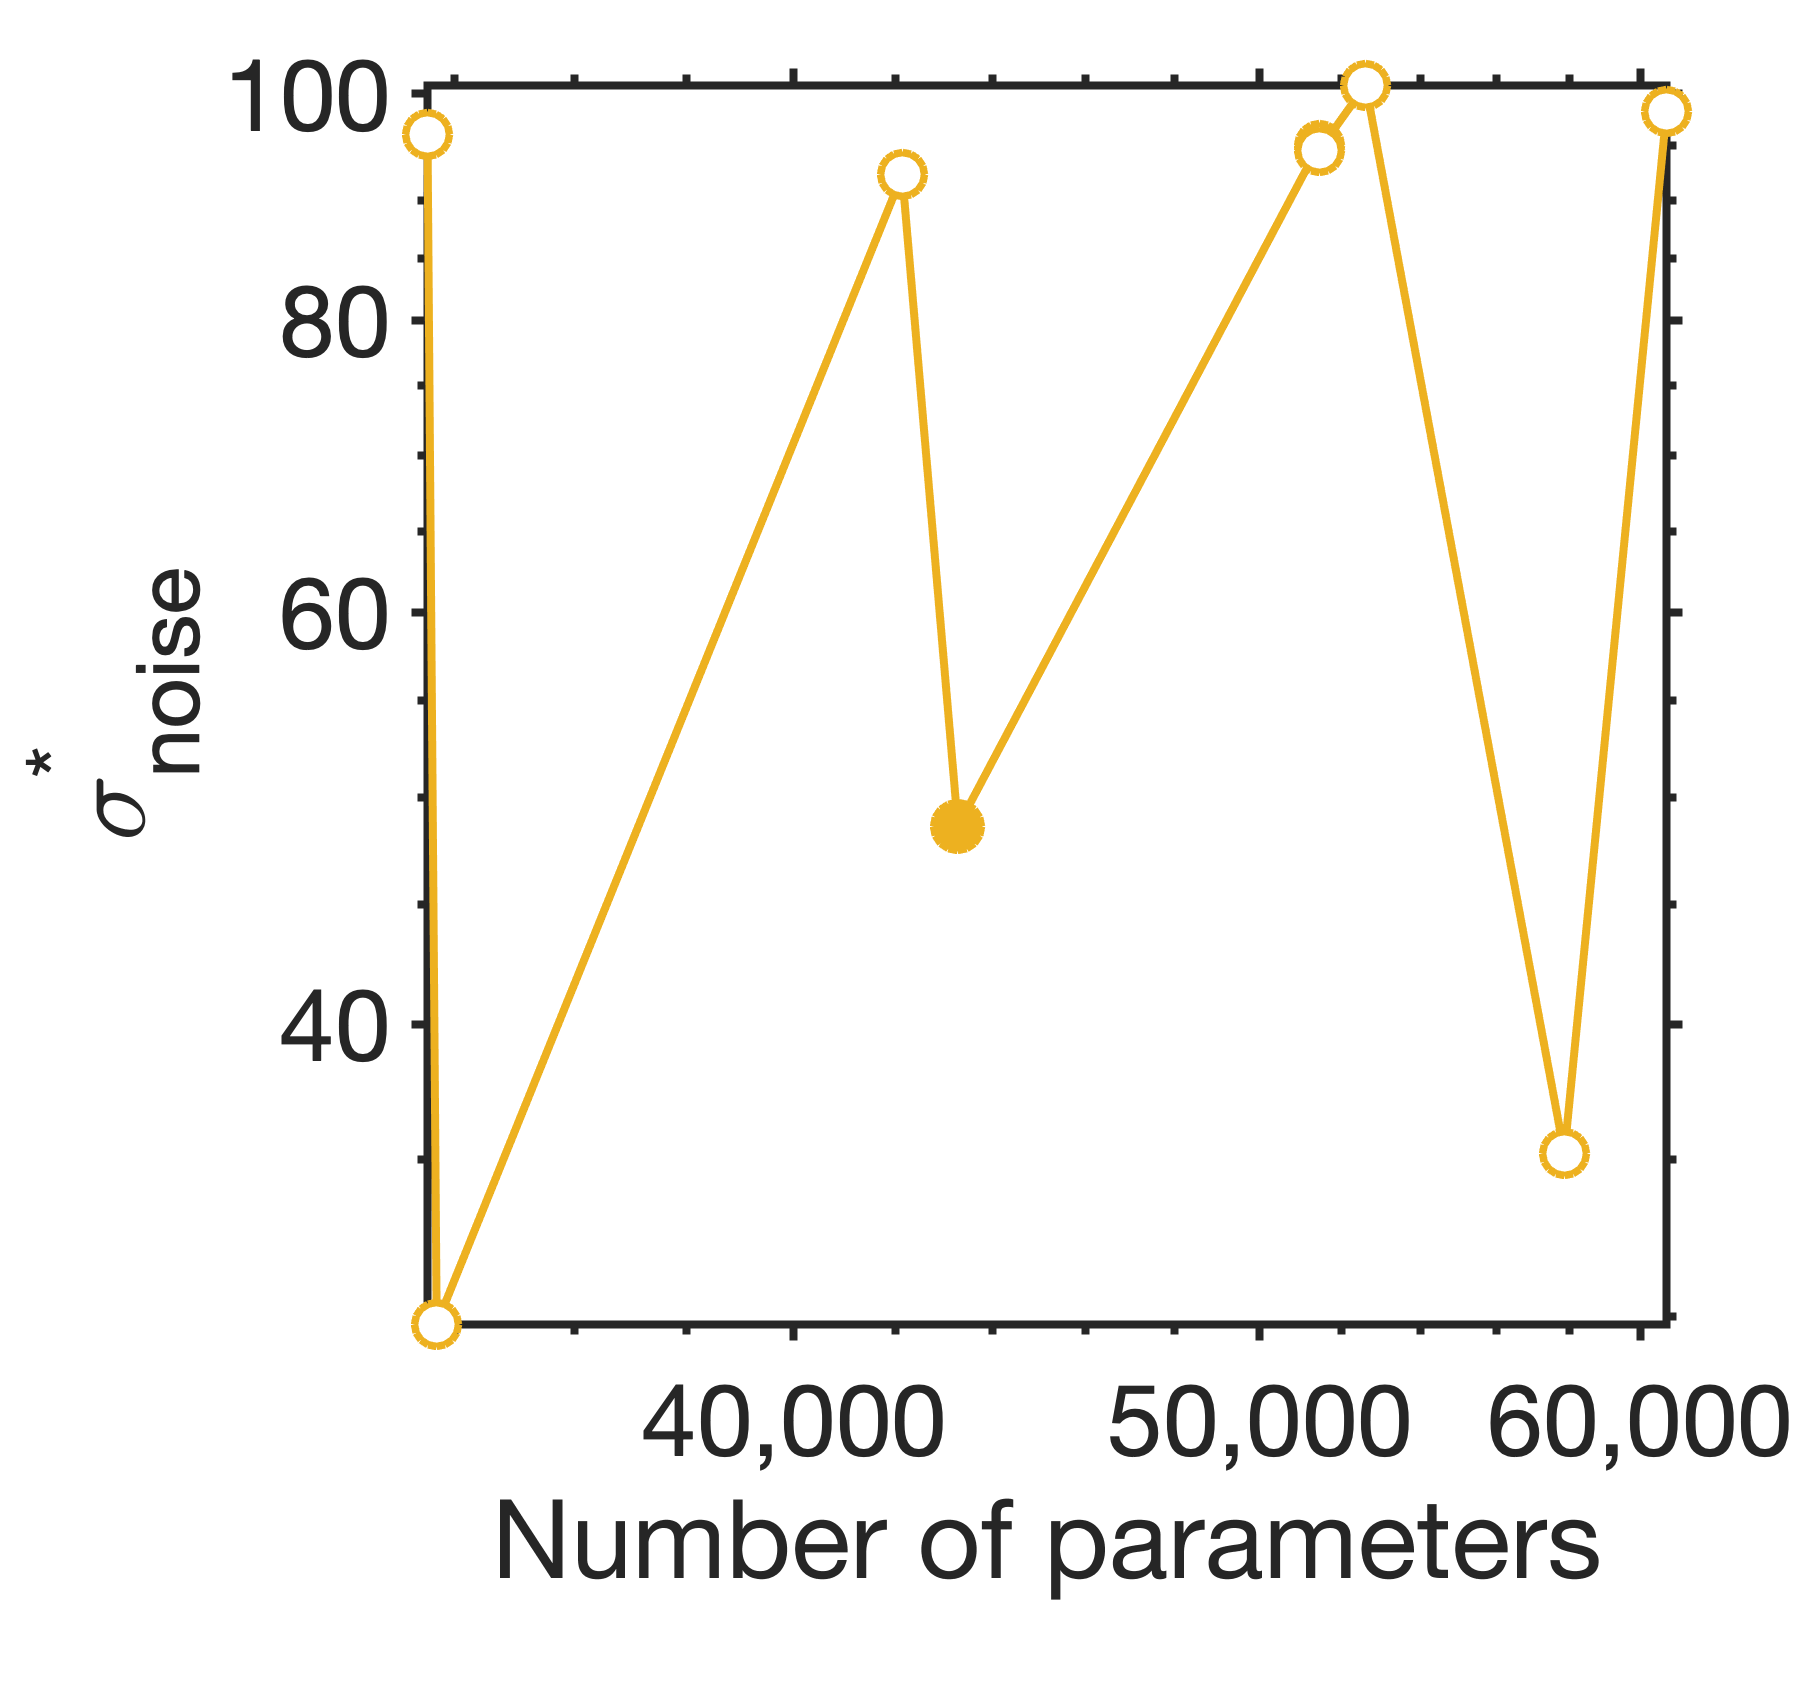
\includegraphics[width=0.19\textwidth]{Figures/Part B/cat2/fold3_noise.png}\hfill
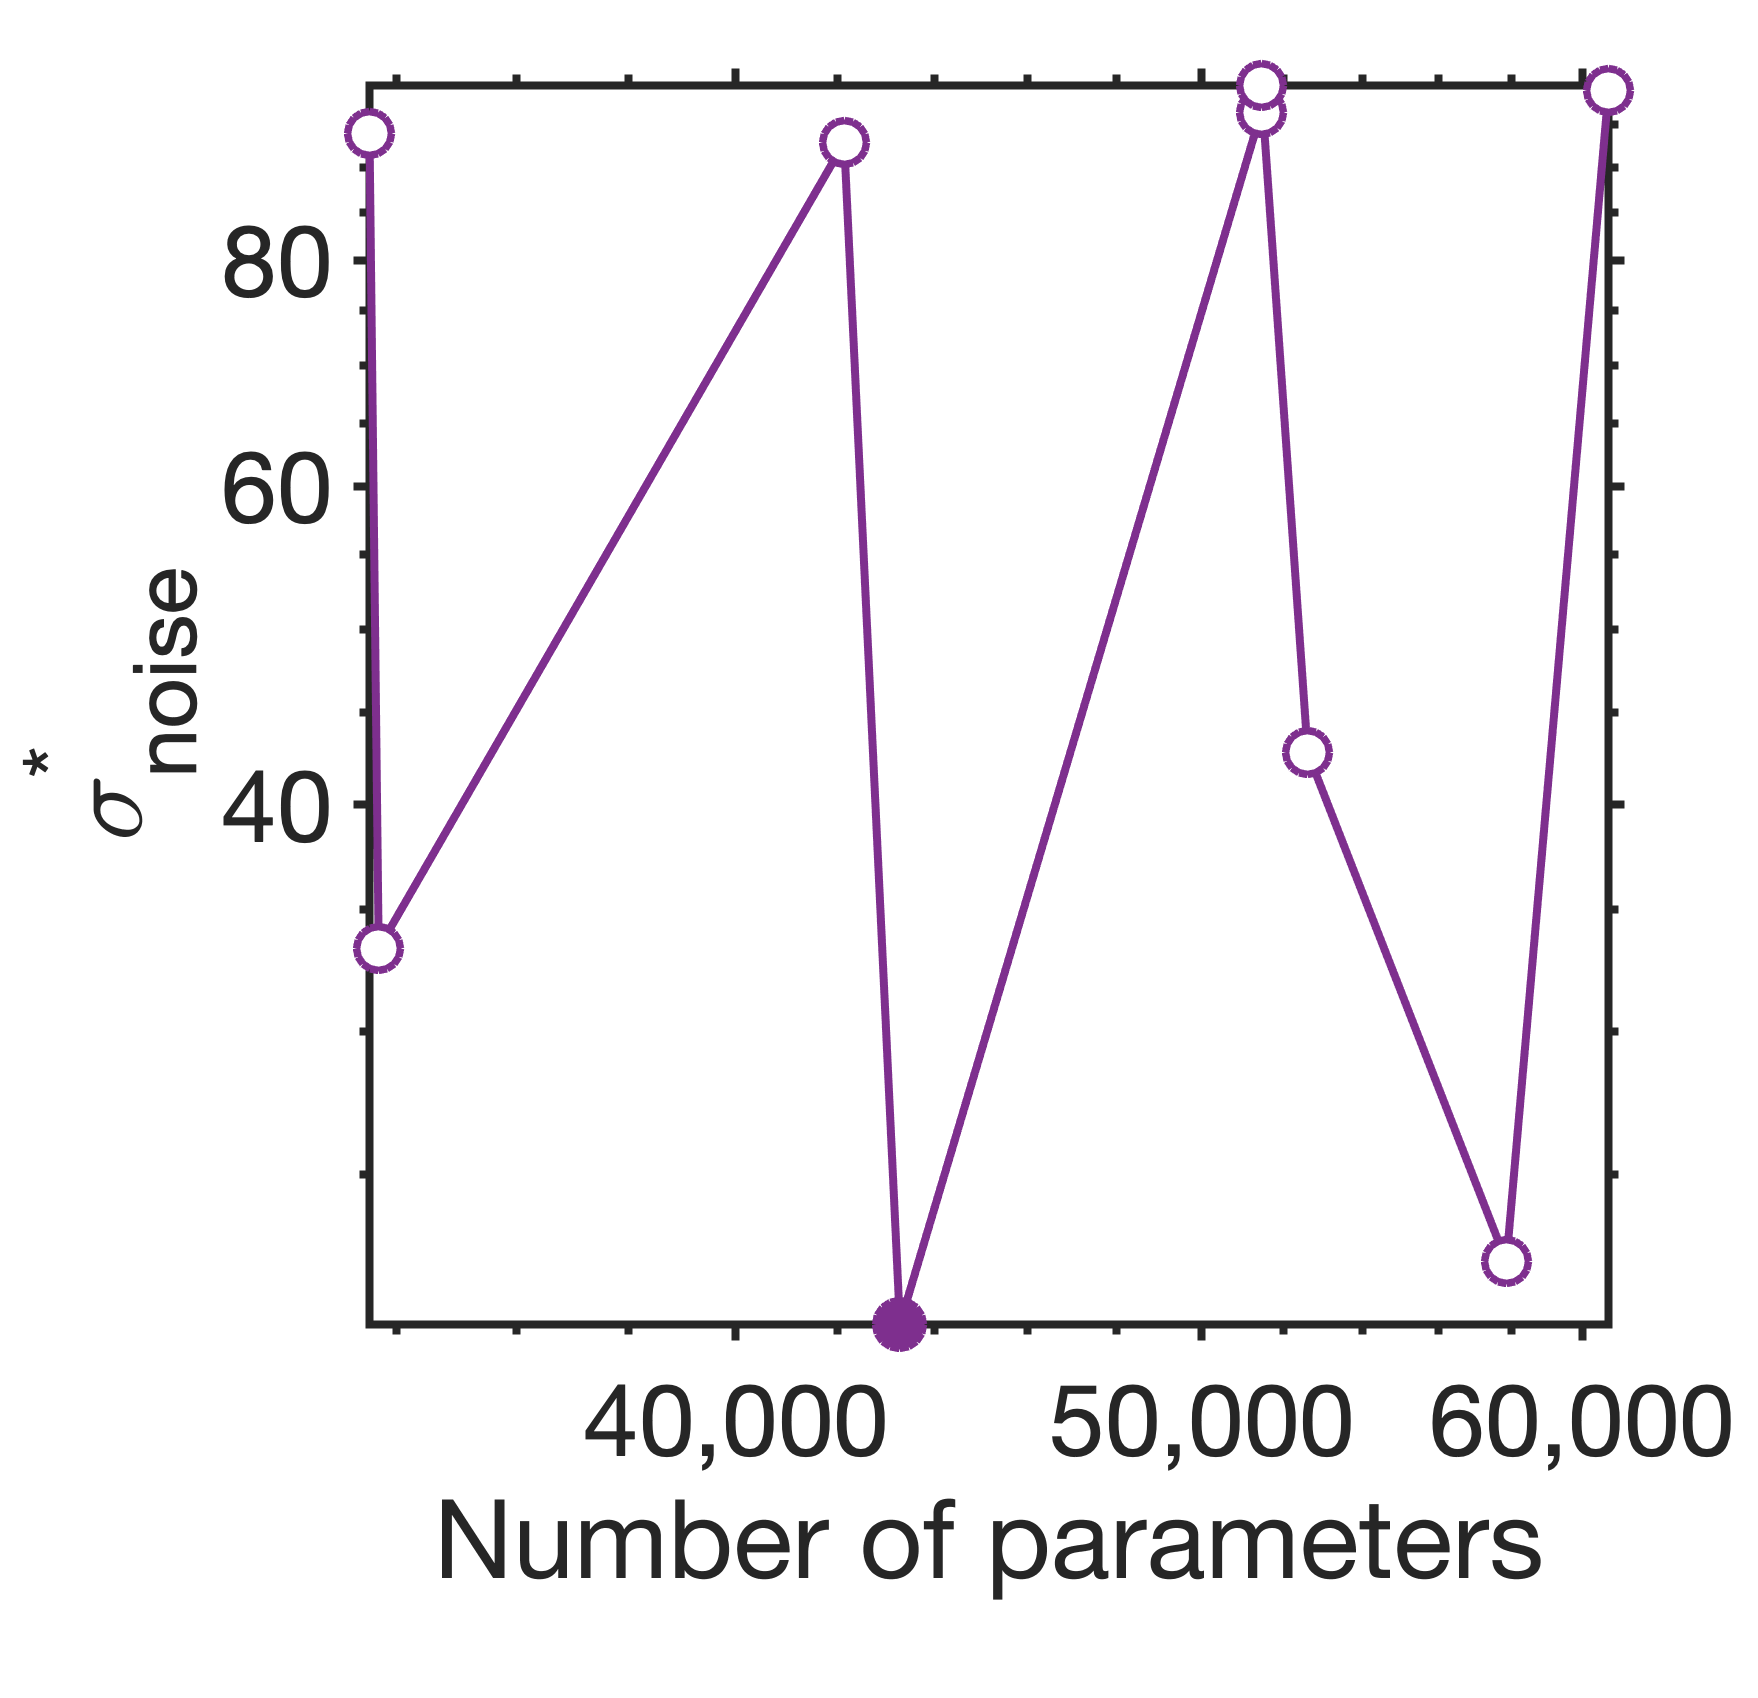
\includegraphics[width=0.19\textwidth]{Figures/Part B/cat2/fold4_noise.png}\hfill
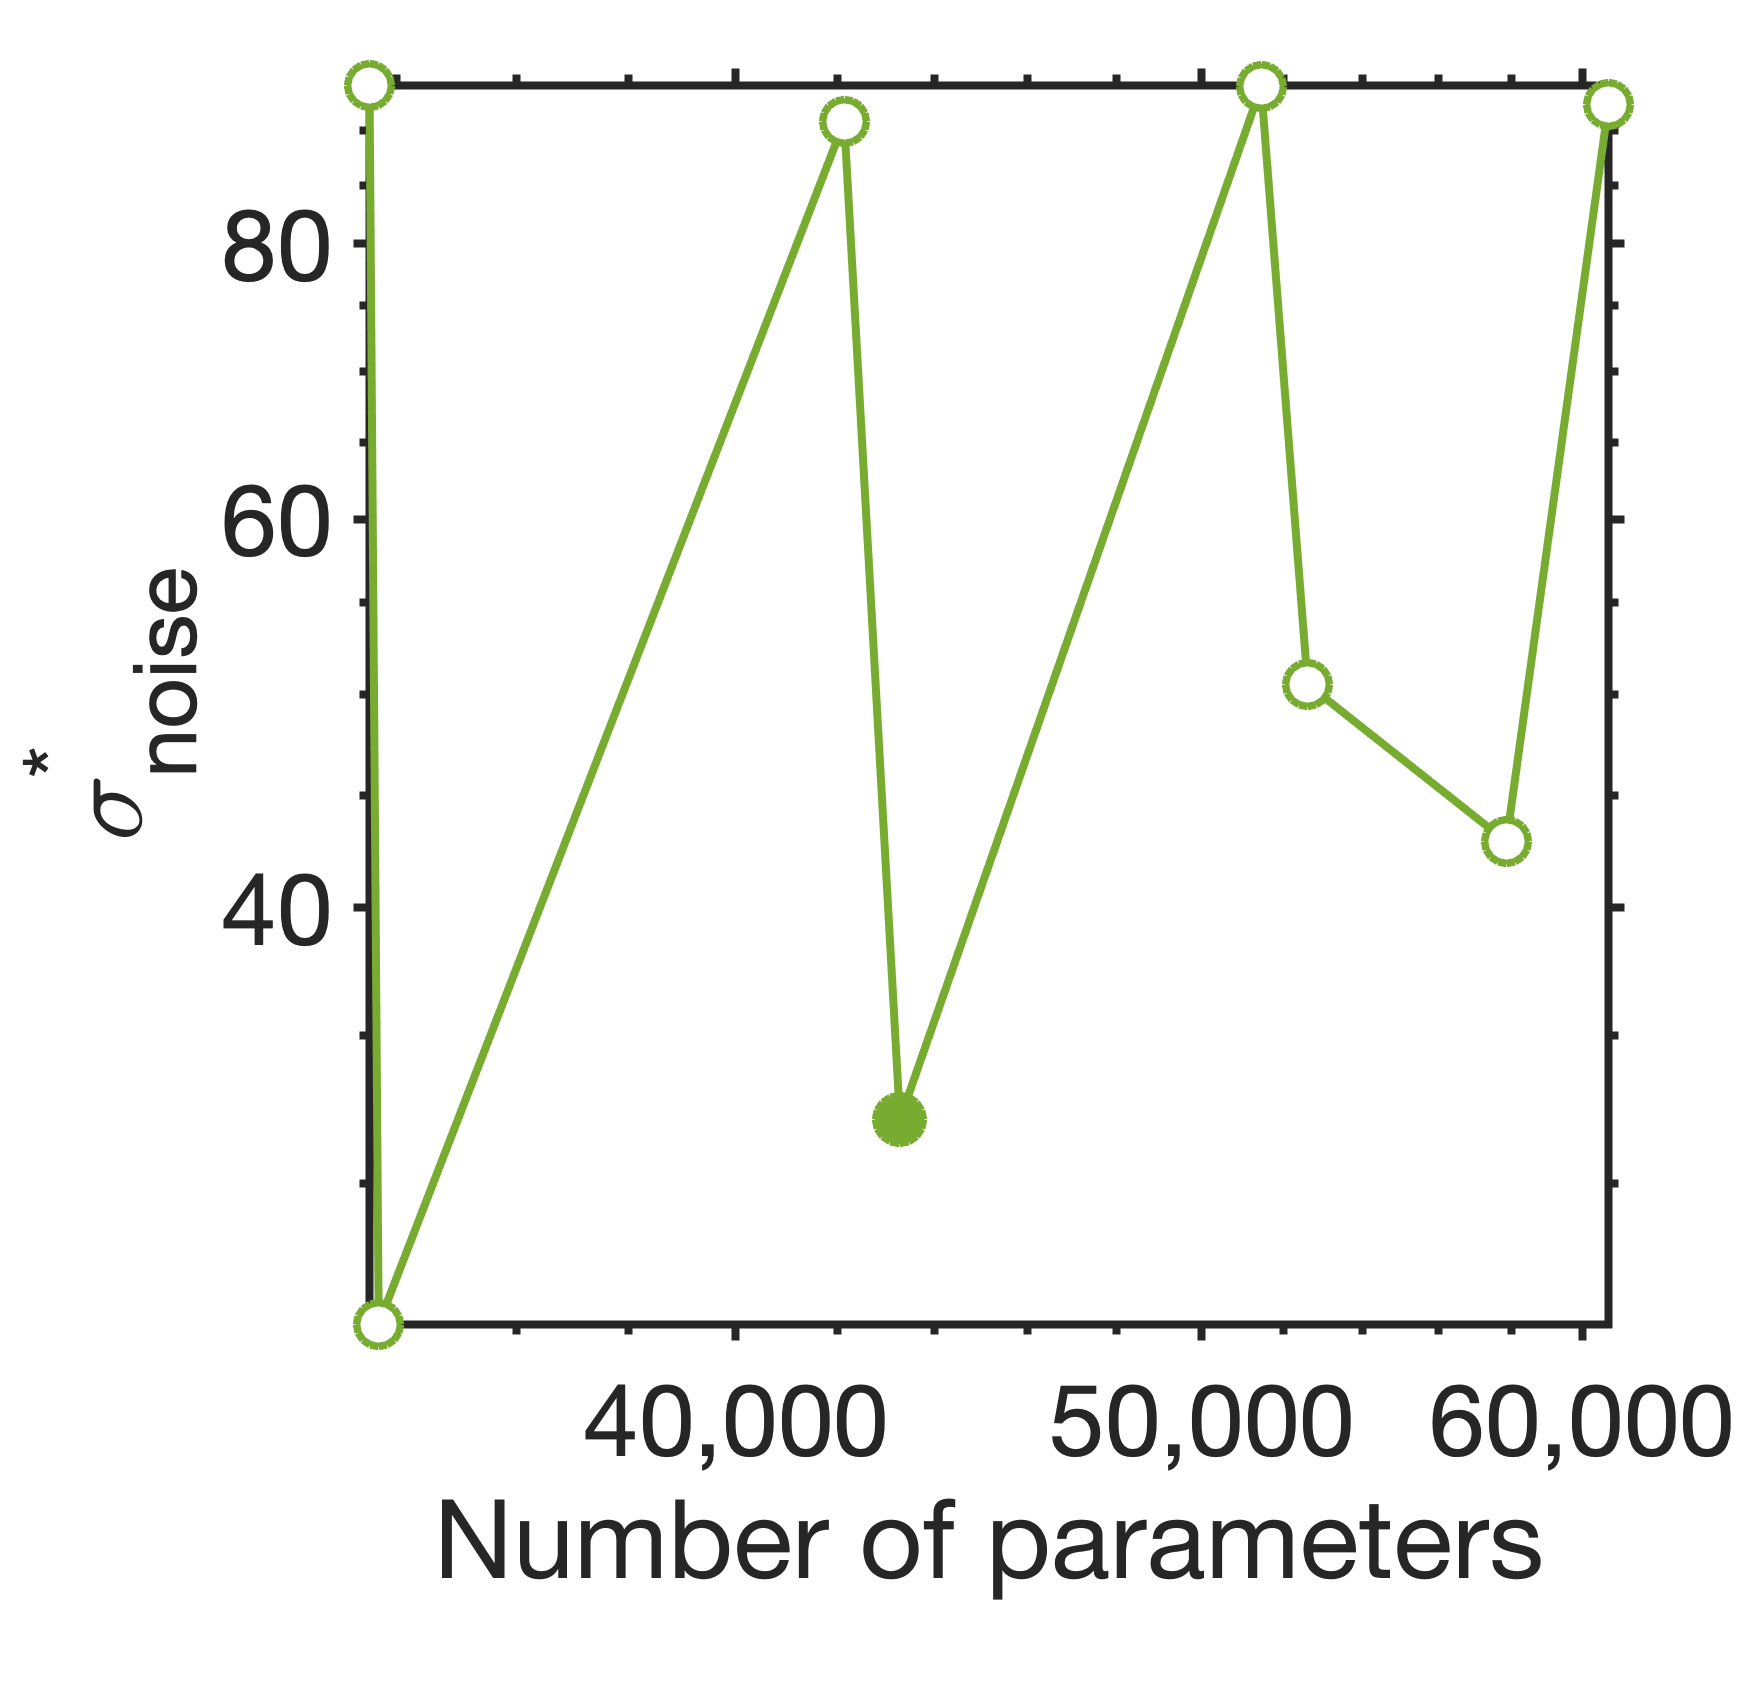
\includegraphics[width=0.19\textwidth]{Figures/Part B/cat2/fold5_noise.png}
\\ (b)
\caption{Level~2 architectures: (a) Posterior plausibility $\rho$ and (b) MAP estimate of $\sigma_{\text{noise}}$ versus model size (number of weight parameters) across cross-validation folds (left to right: folds 1–5).
}
\label{fig:cat2_plausibility_sigma}
\end{figure}


%-- Level 2: validation
The top-ranked architectures in each fold are then evaluated on the held-out subjects using the validation protocol. While Level~2 models exhibit improved predictive performance, most candidates still violate the NLPD tolerance in a subset of one-hour windows, leading to rejection. Representative failure cases (Figure ~\ref{fig:level2_falied}) show that these violations are primarily concentrated around postprandial phases.
EVIDENT, however, identifies a single architecture, \(Level_2Arch_4\), that satisfies the validation criterion across all folds and held-out subjects. As shown in Figure~\ref{fig:level2_success}, this model produces consistent one-hour forecasts that remain within the prescribed tolerance across all validation windows. This architecture is therefore selected as the trustworthy predictor.


\begin{figure}[!ht]
\centering
\begin{minipage}[t]{0.48\textwidth}
  \centering
  \includegraphics[width=\linewidth]{Figures/Part B/cat2/p9_c2.png}
  \caption*{(a)}
\end{minipage}\hfill
\begin{minipage}[t]{0.48\textwidth}
  \centering
  \includegraphics[width=\linewidth]{Figures/Part B/cat2/p10_c2.png}
  \caption*{(b)}
\end{minipage}
\caption{Representative validation failures for a Level~2 architecture ($Level_2Arch_2$) on held-out patients. (a) Patient 9 and (b) Patient 10 from fold~1. 
Red segments indicate one-hour prediction windows that violates the acceptance criterion $NLPD \leq Tol$.}
\label{fig:level2_falied}
\end{figure}



\begin{figure}[!ht]
\centering
\begin{minipage}[t]{0.48\textwidth}
  \centering
  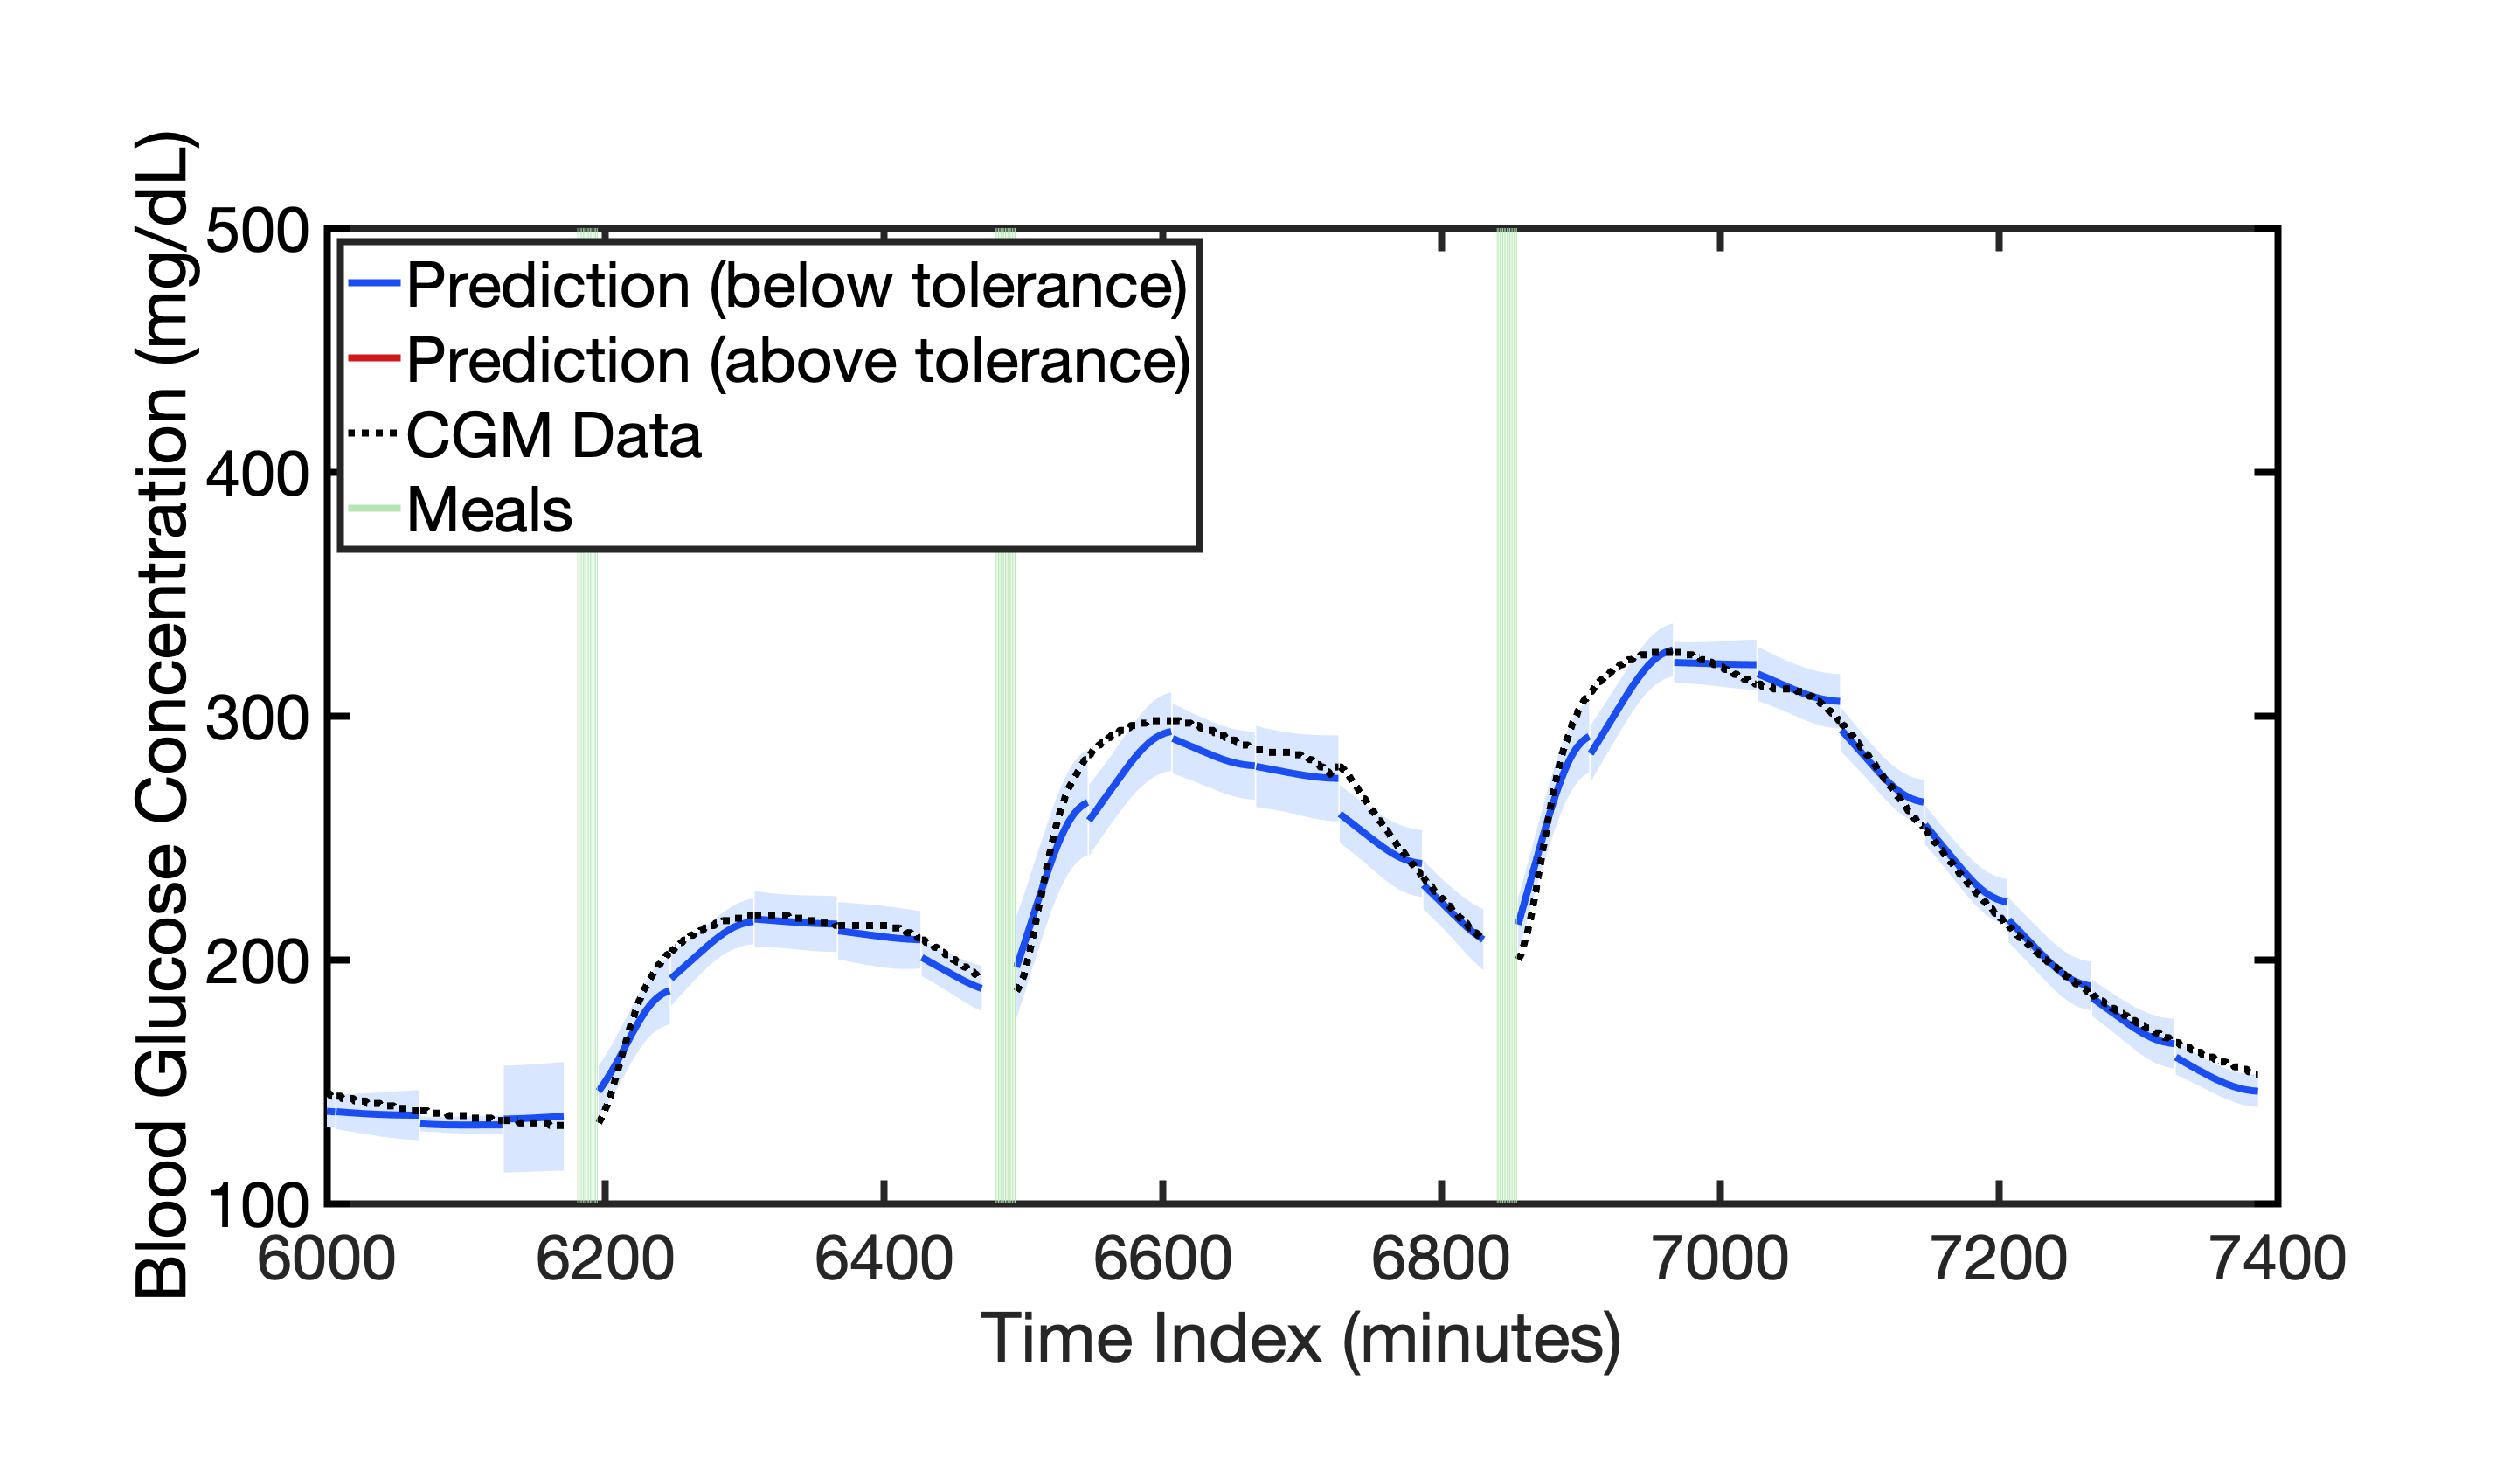
\includegraphics[width=\linewidth]{Figures/Part B/cat2/p1_c2.png}
  \caption*{(a)}
\end{minipage}\hfill
\begin{minipage}[t]{0.48\textwidth}
  \centering
  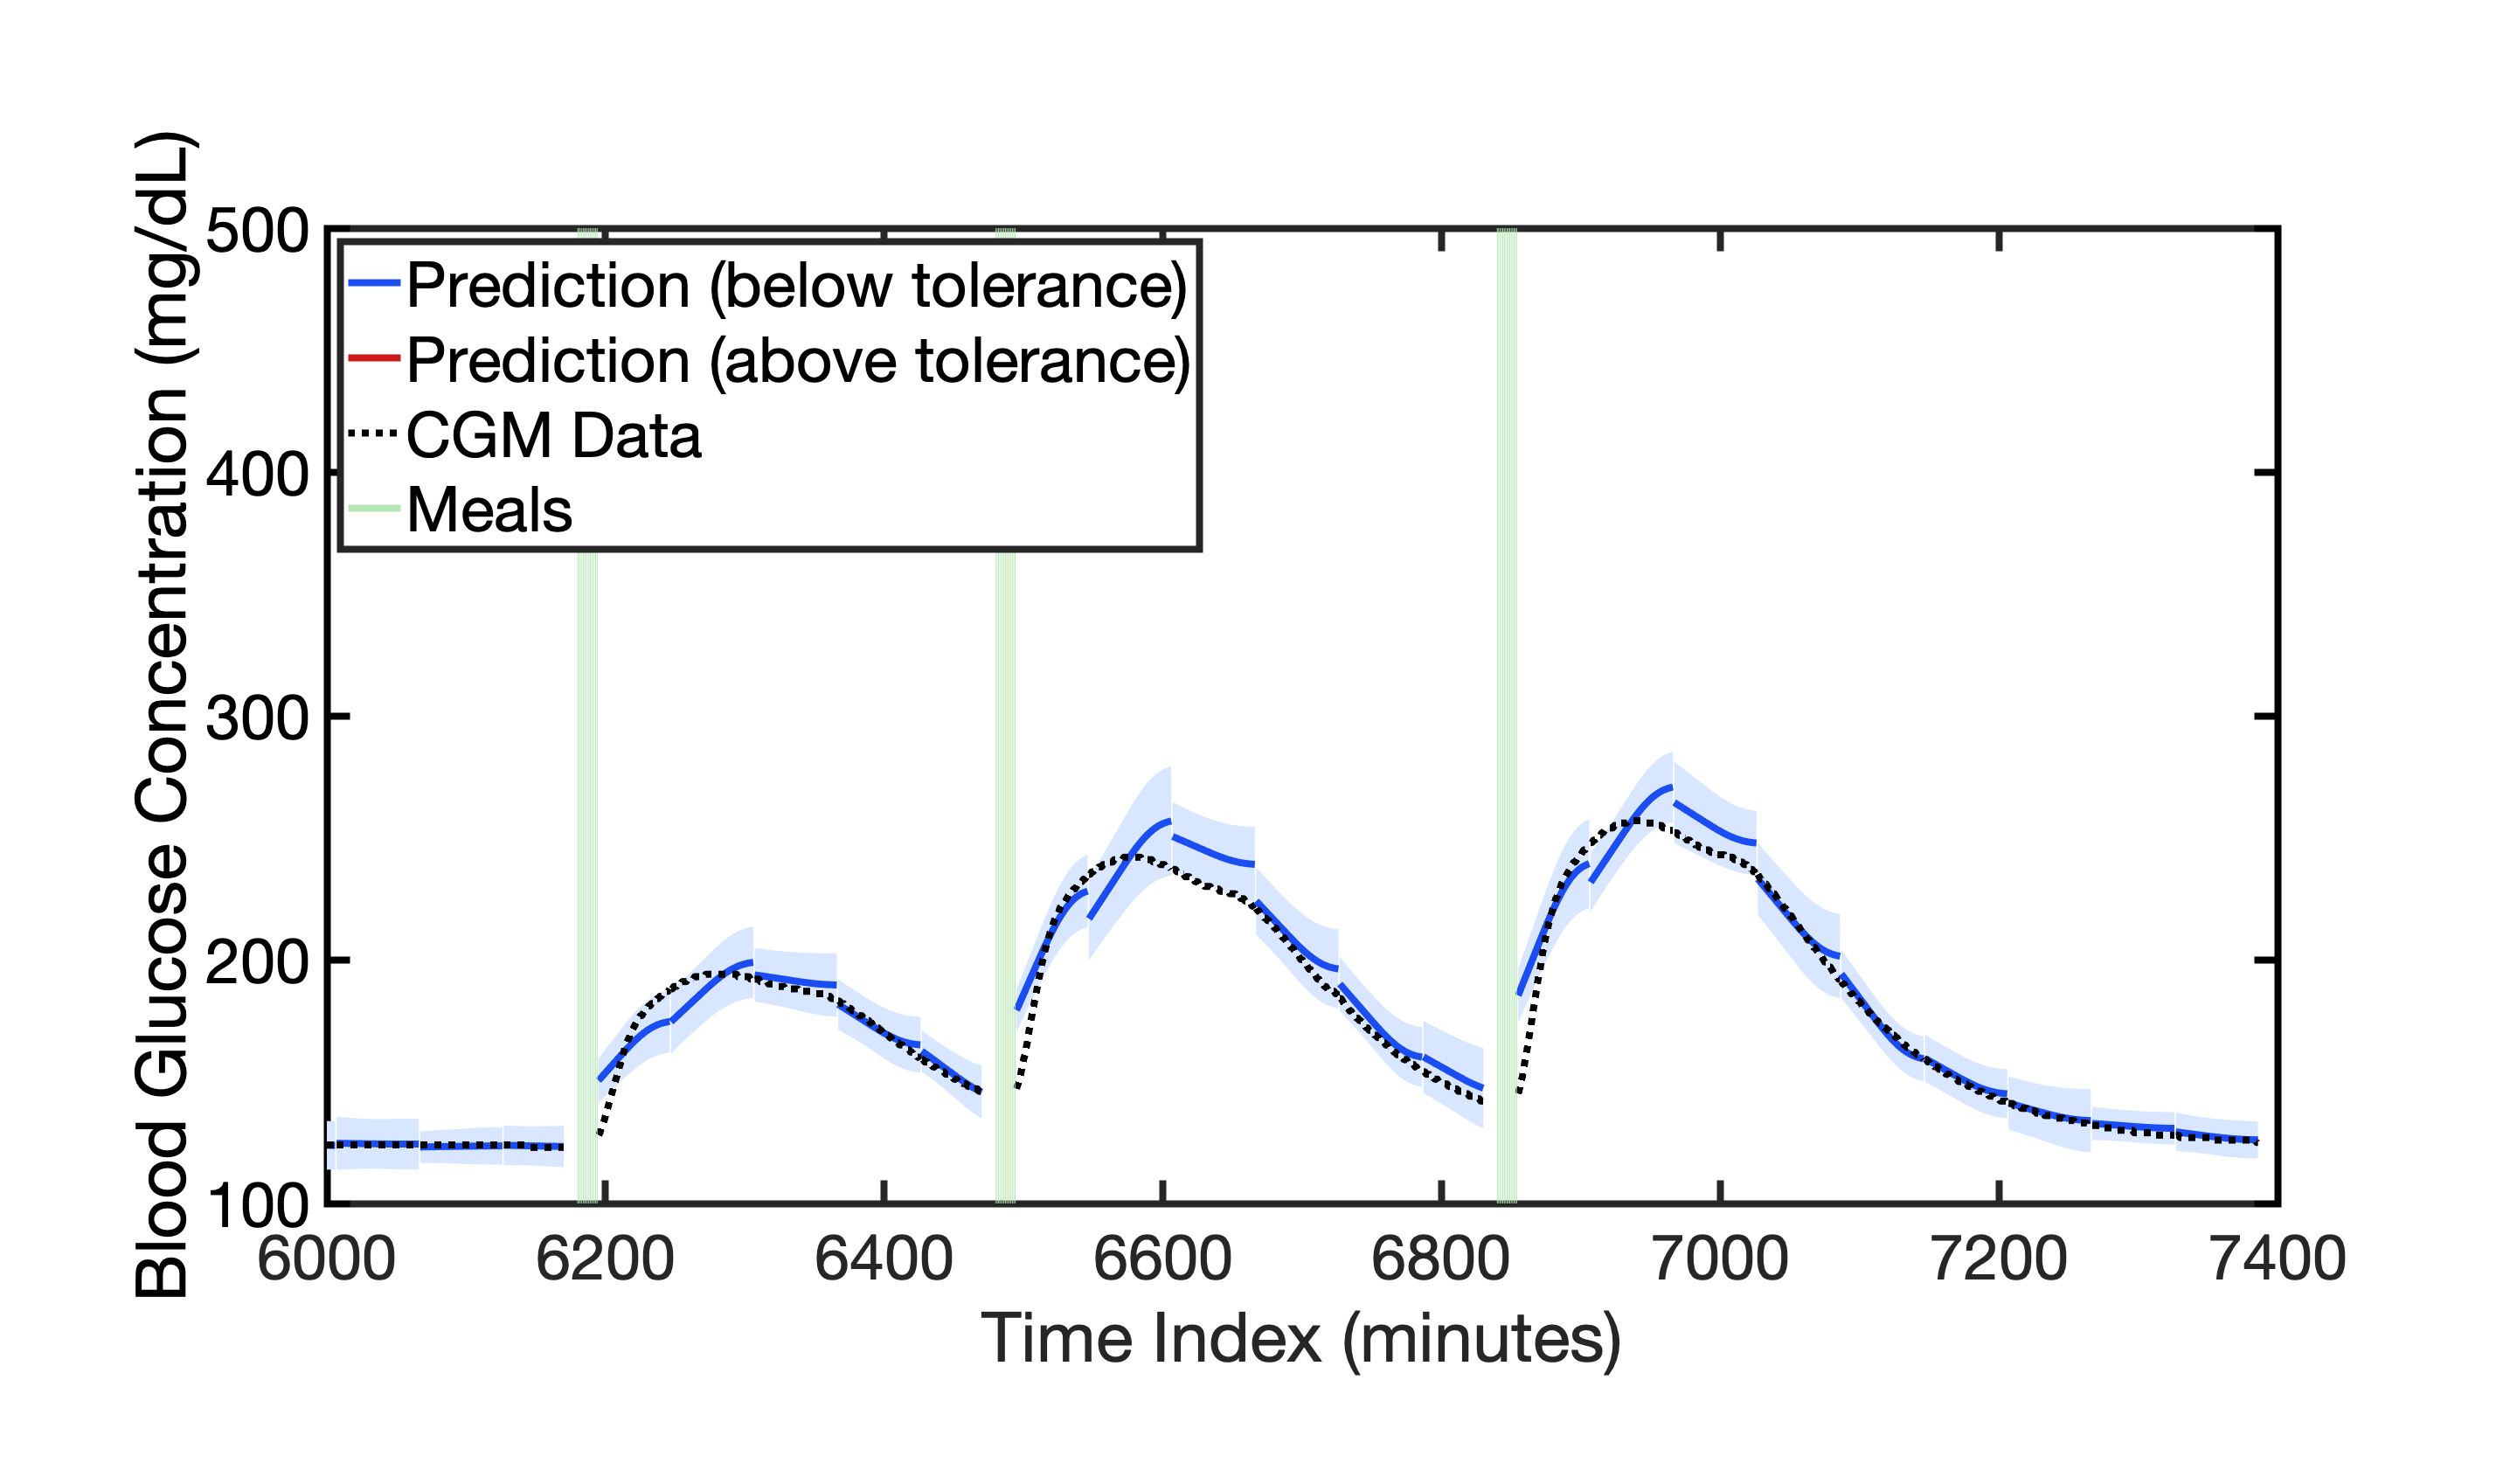
\includegraphics[width=\linewidth]{Figures/Part B/cat2/p2_c2.png}
  \caption*{(b)}
\end{minipage}
\begin{minipage}[t]{0.48\textwidth}
  \centering
  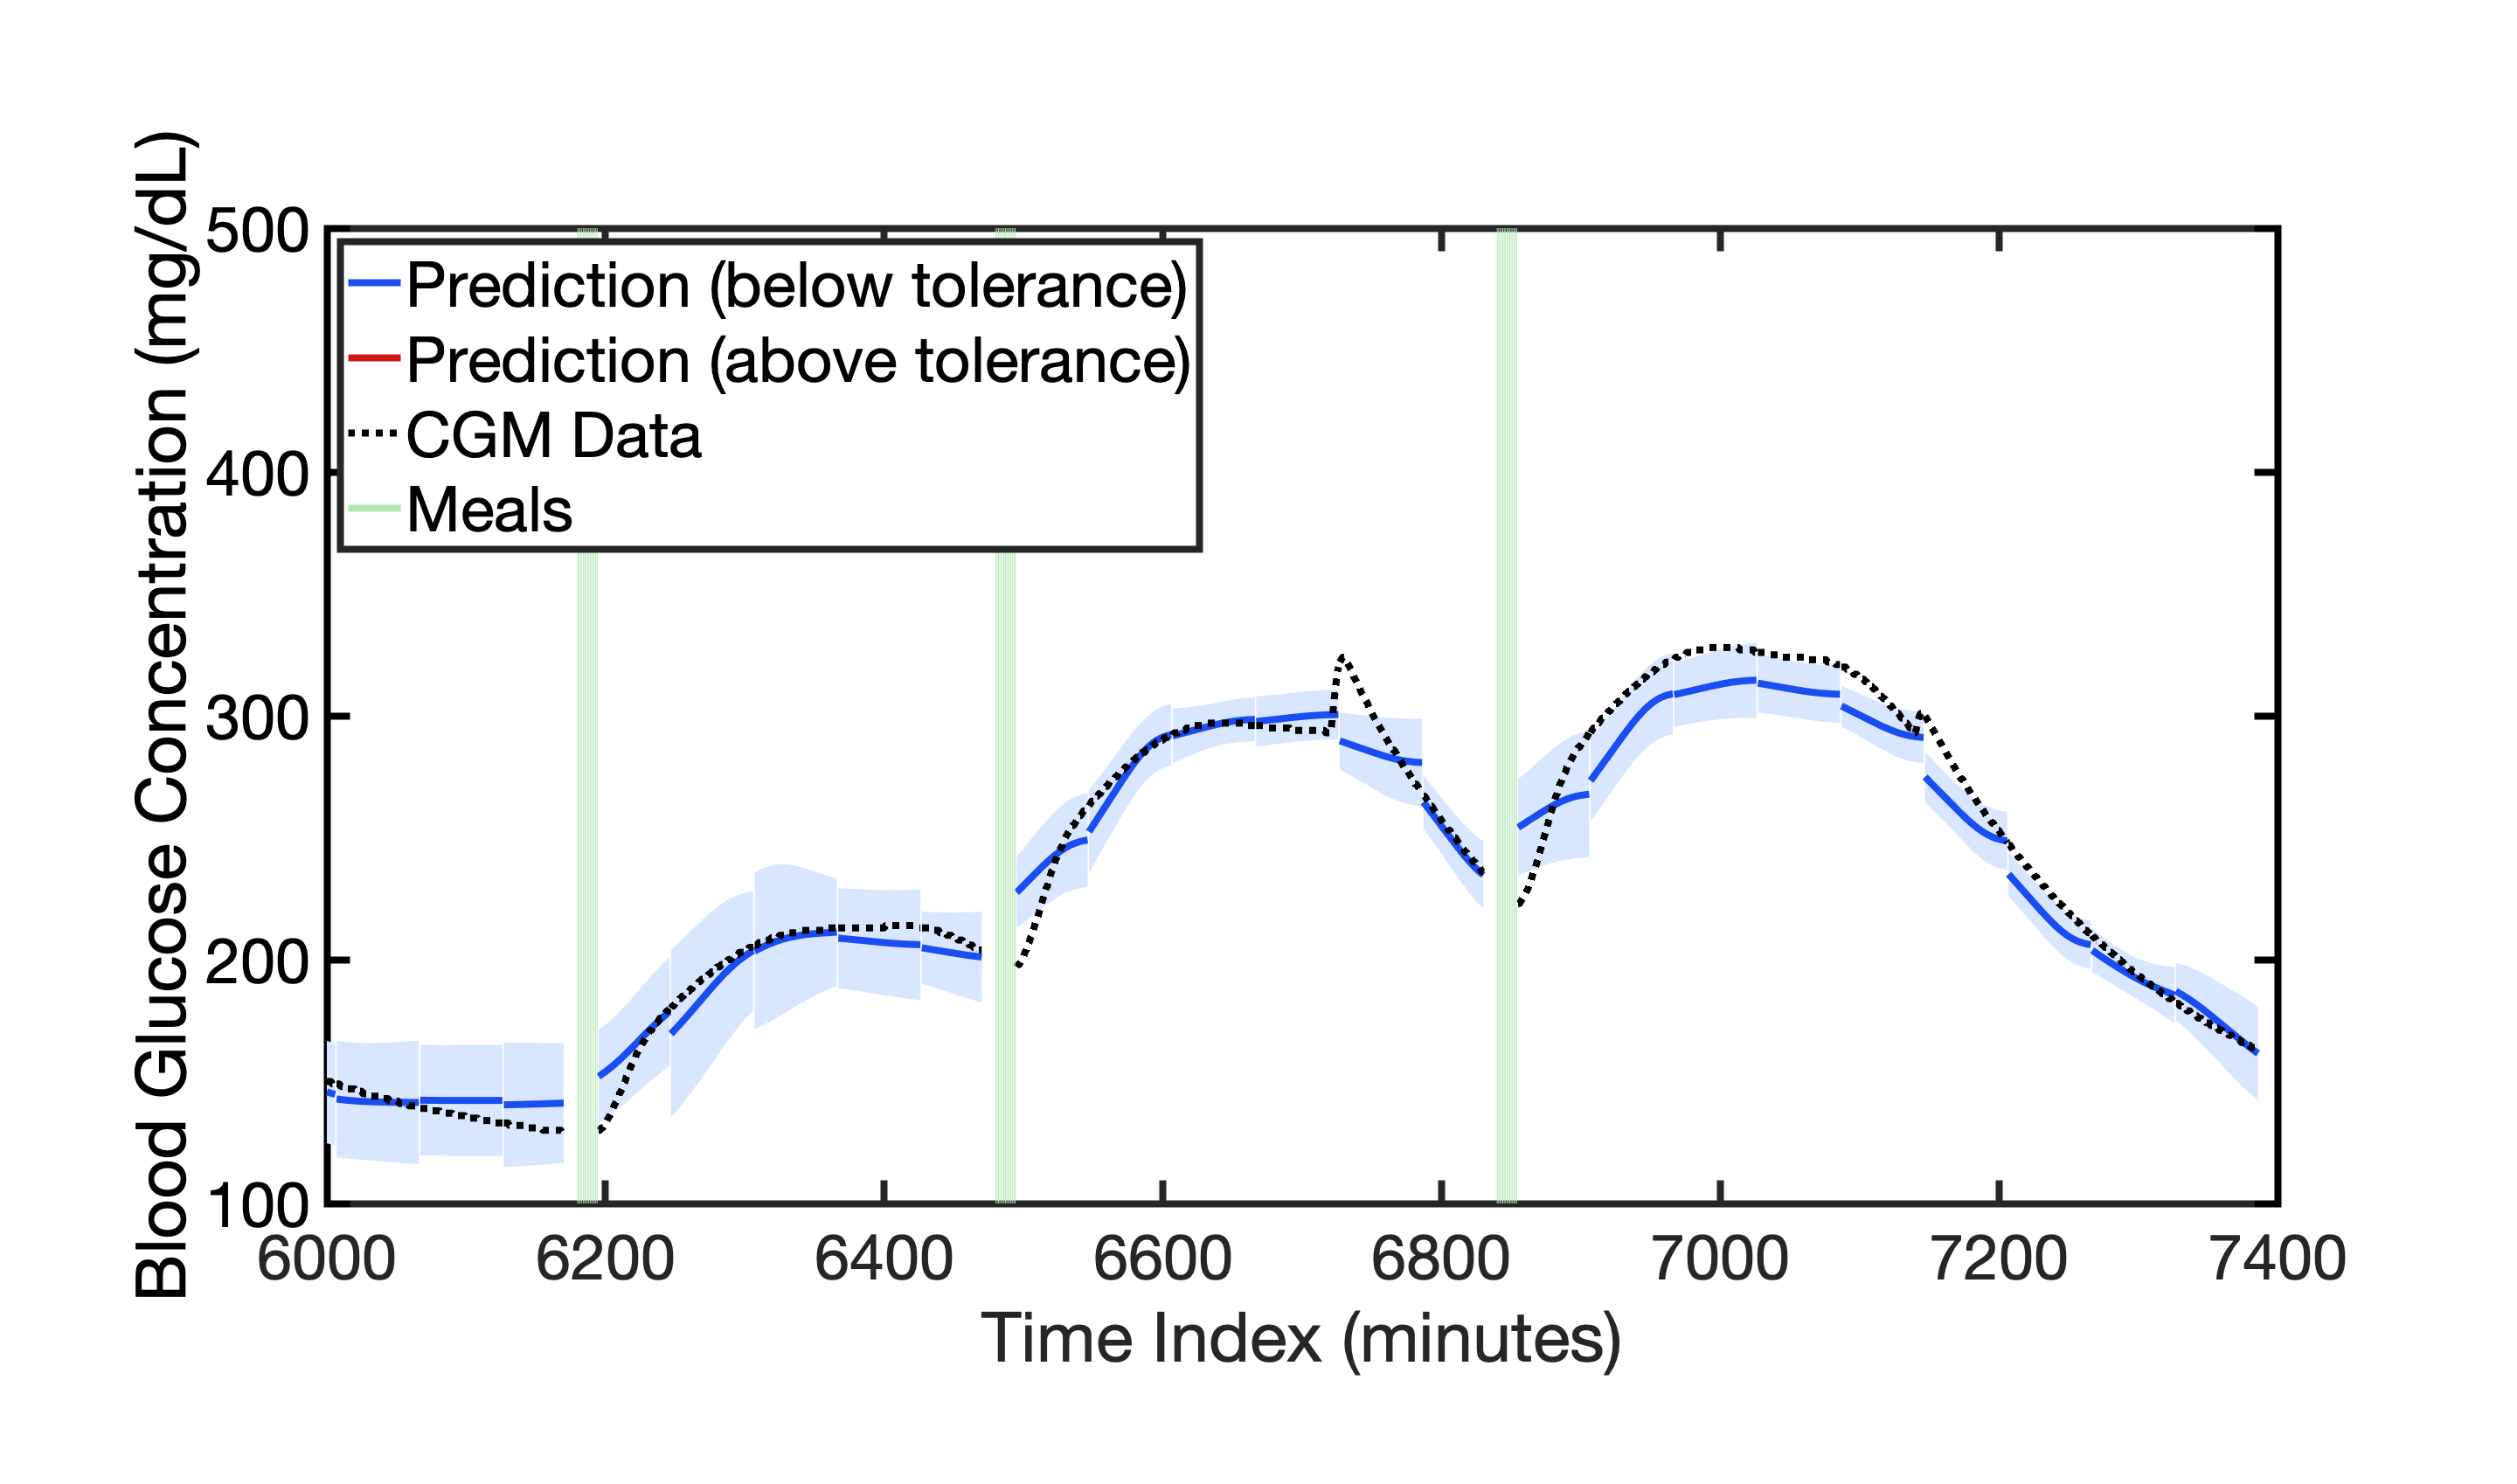
\includegraphics[width=\linewidth]{Figures/Part B/cat2/p3_c2.png}
  \caption*{(c)}
\end{minipage}\hfill
\begin{minipage}[t]{0.48\textwidth}
  \centering
  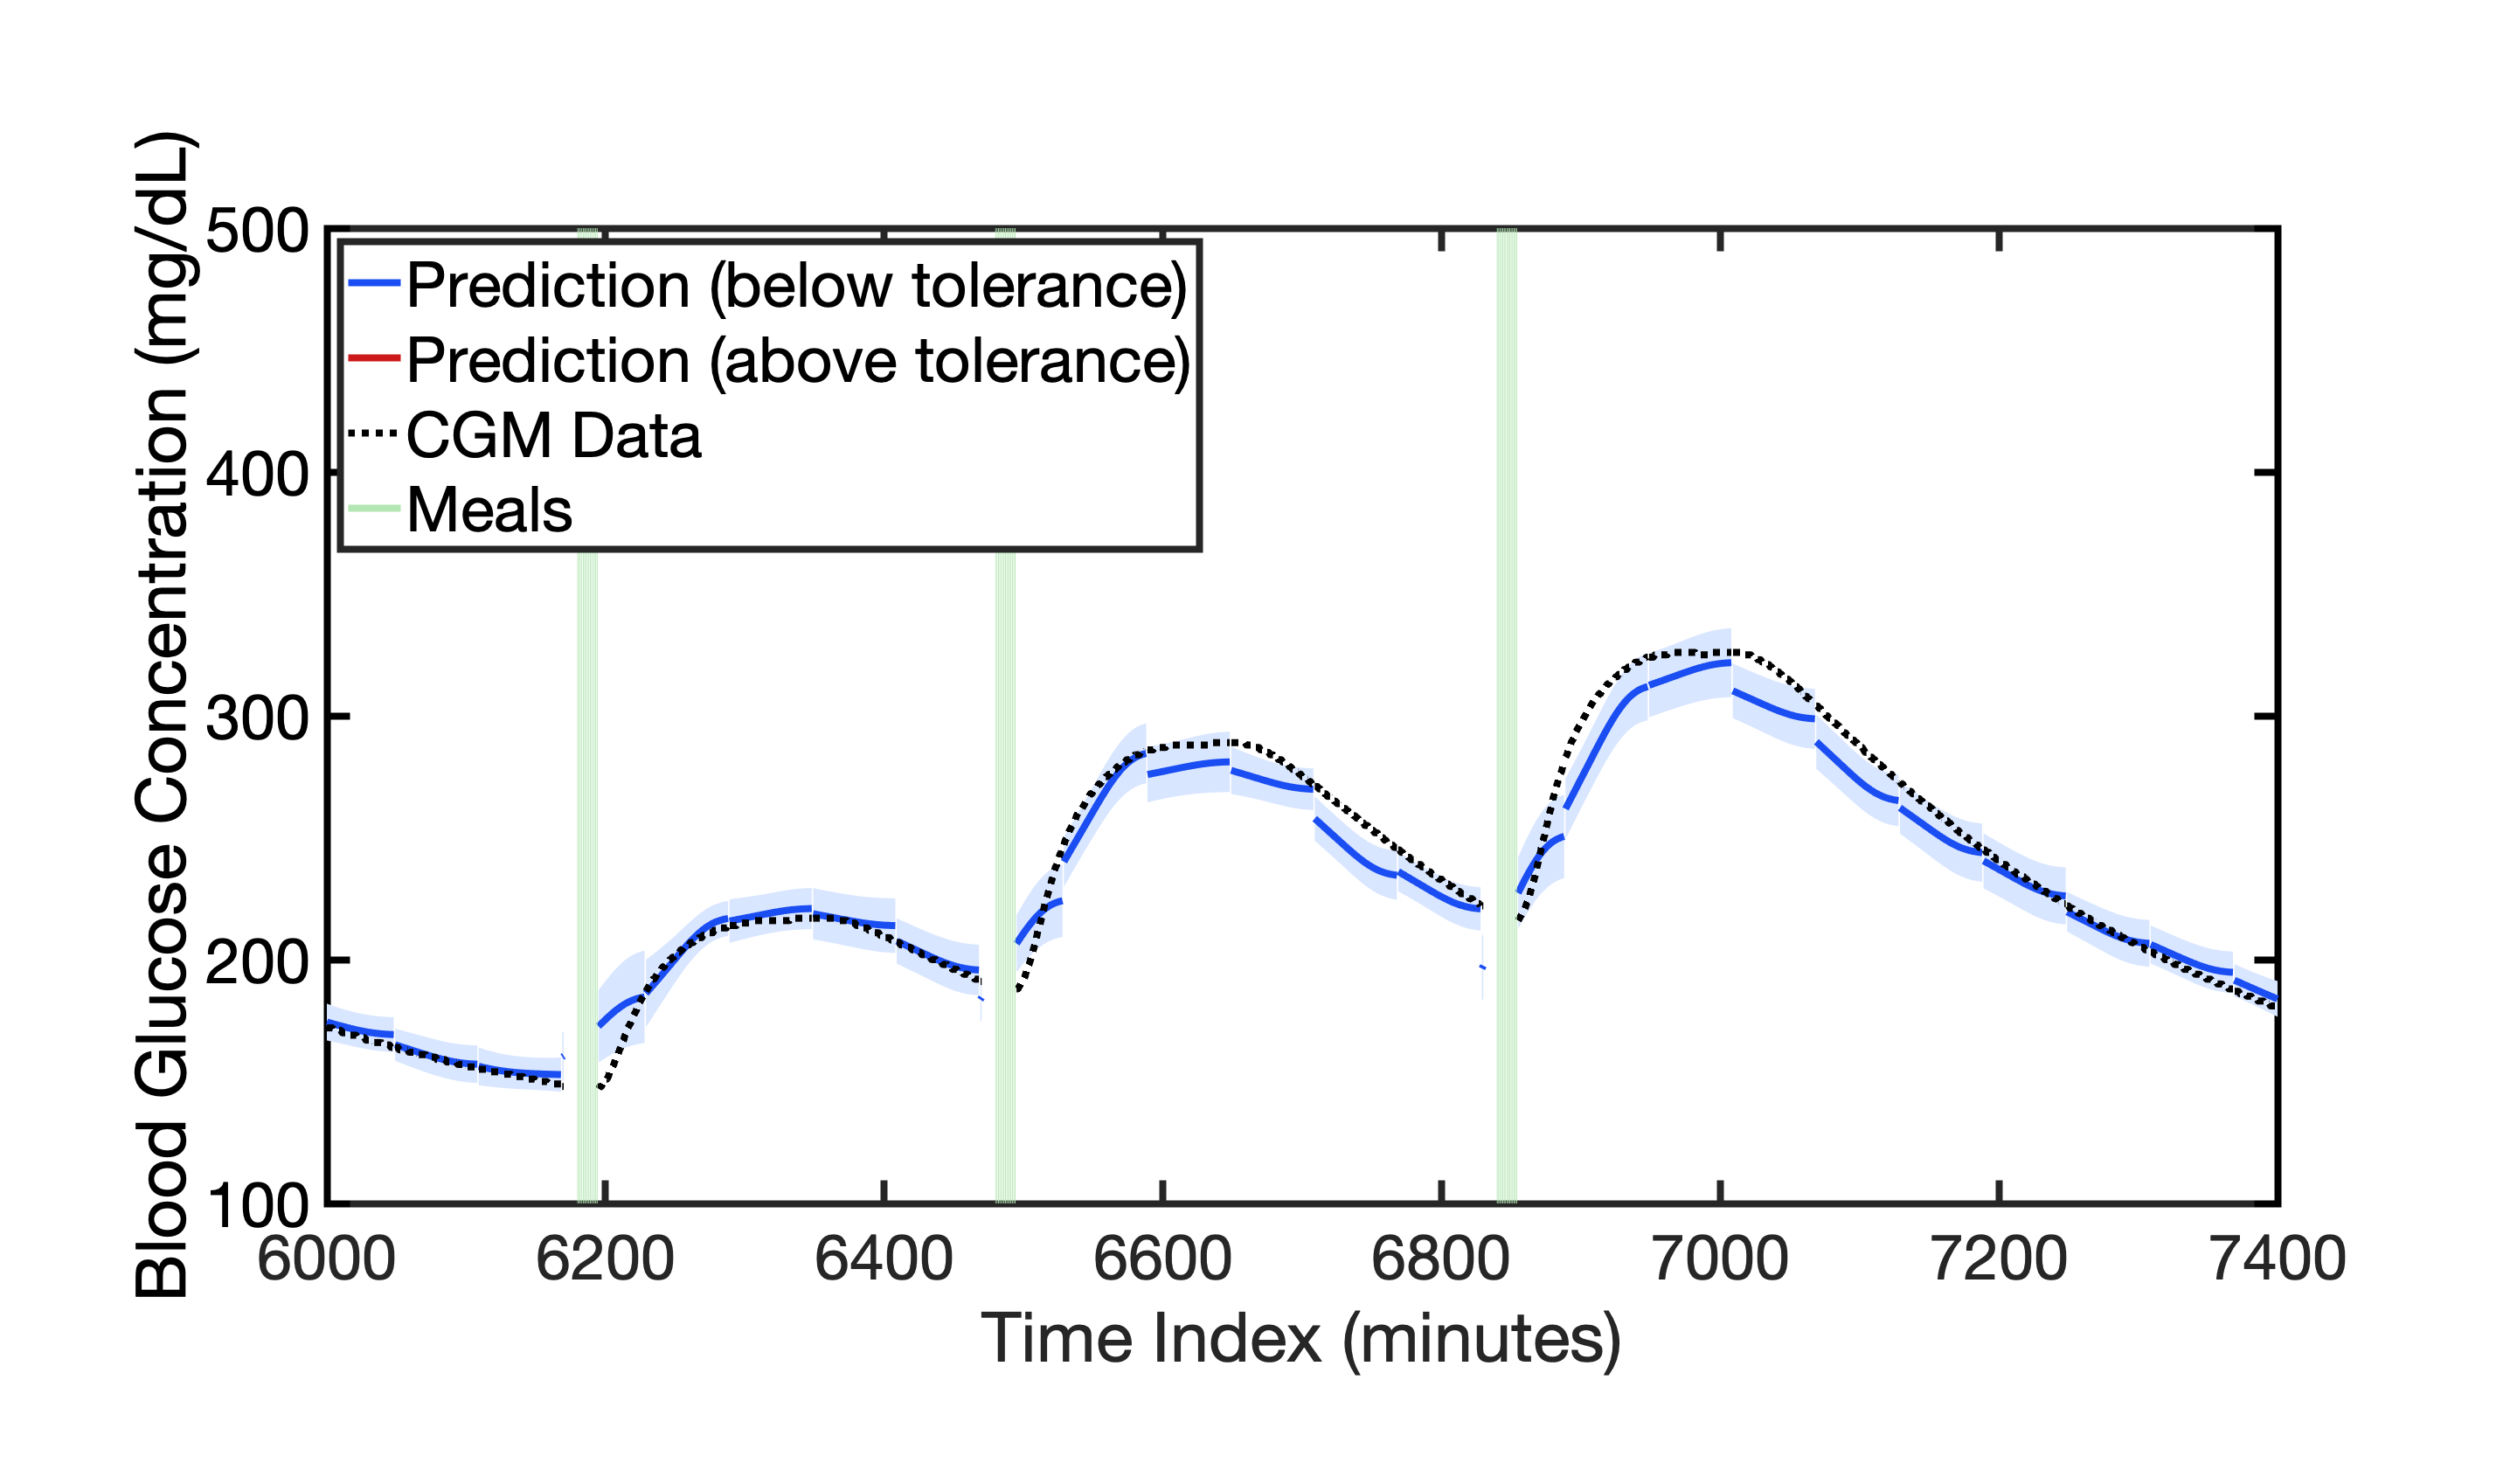
\includegraphics[width=\linewidth]{Figures/Part B/cat2/p4_c2.png}
  \caption*{(d)}
\end{minipage}
\caption{Validation results for the selected Level~2 architecture ($Level_2Arch_4$) across multiple folds and held-out patients. (a–b) Patients 1–2 from fold~3 and (c–d) Patients 3–4 from fold~4. The model produces accurate and reliable one-hour forecasts that remain within the NLPD tolerance across all validation windows, demonstrating EVIDENT identified trustworthy predictor.}
\label{fig:level2_success}
\end{figure}


% -- Level 2: BMA
In addition to single-architecture selection, EVIDENT also supports a plausibility-weighted ensemble predictor when multiple architectures remain competitive. To assess this, we compare the predictions of the most plausible architecture with the ensemble prediction defined in \eqref{eq:bma} over all Level~2 architectures for fold~2 (Figure~\ref{fig:bma}).
The ensemble achieves improved predictive accuracy and lower NLPD relative to individual architectures, while producing wider uncertainty bands due to aggregation across models. This behavior reflects an ensemble effect, where different architectures capture complementary temporal patterns and their combination mitigates individual model deficiencies. These results indicate that, although a single architecture can satisfy the validation criterion, the plausibility-weighted ensemble provides a mechanism for improving predictive performance while more fully capturing model uncertainty in the presence of multiple candidates.

\begin{figure}[!ht]
\centering
\begin{minipage}[t]{0.48\textwidth}
  \centering
  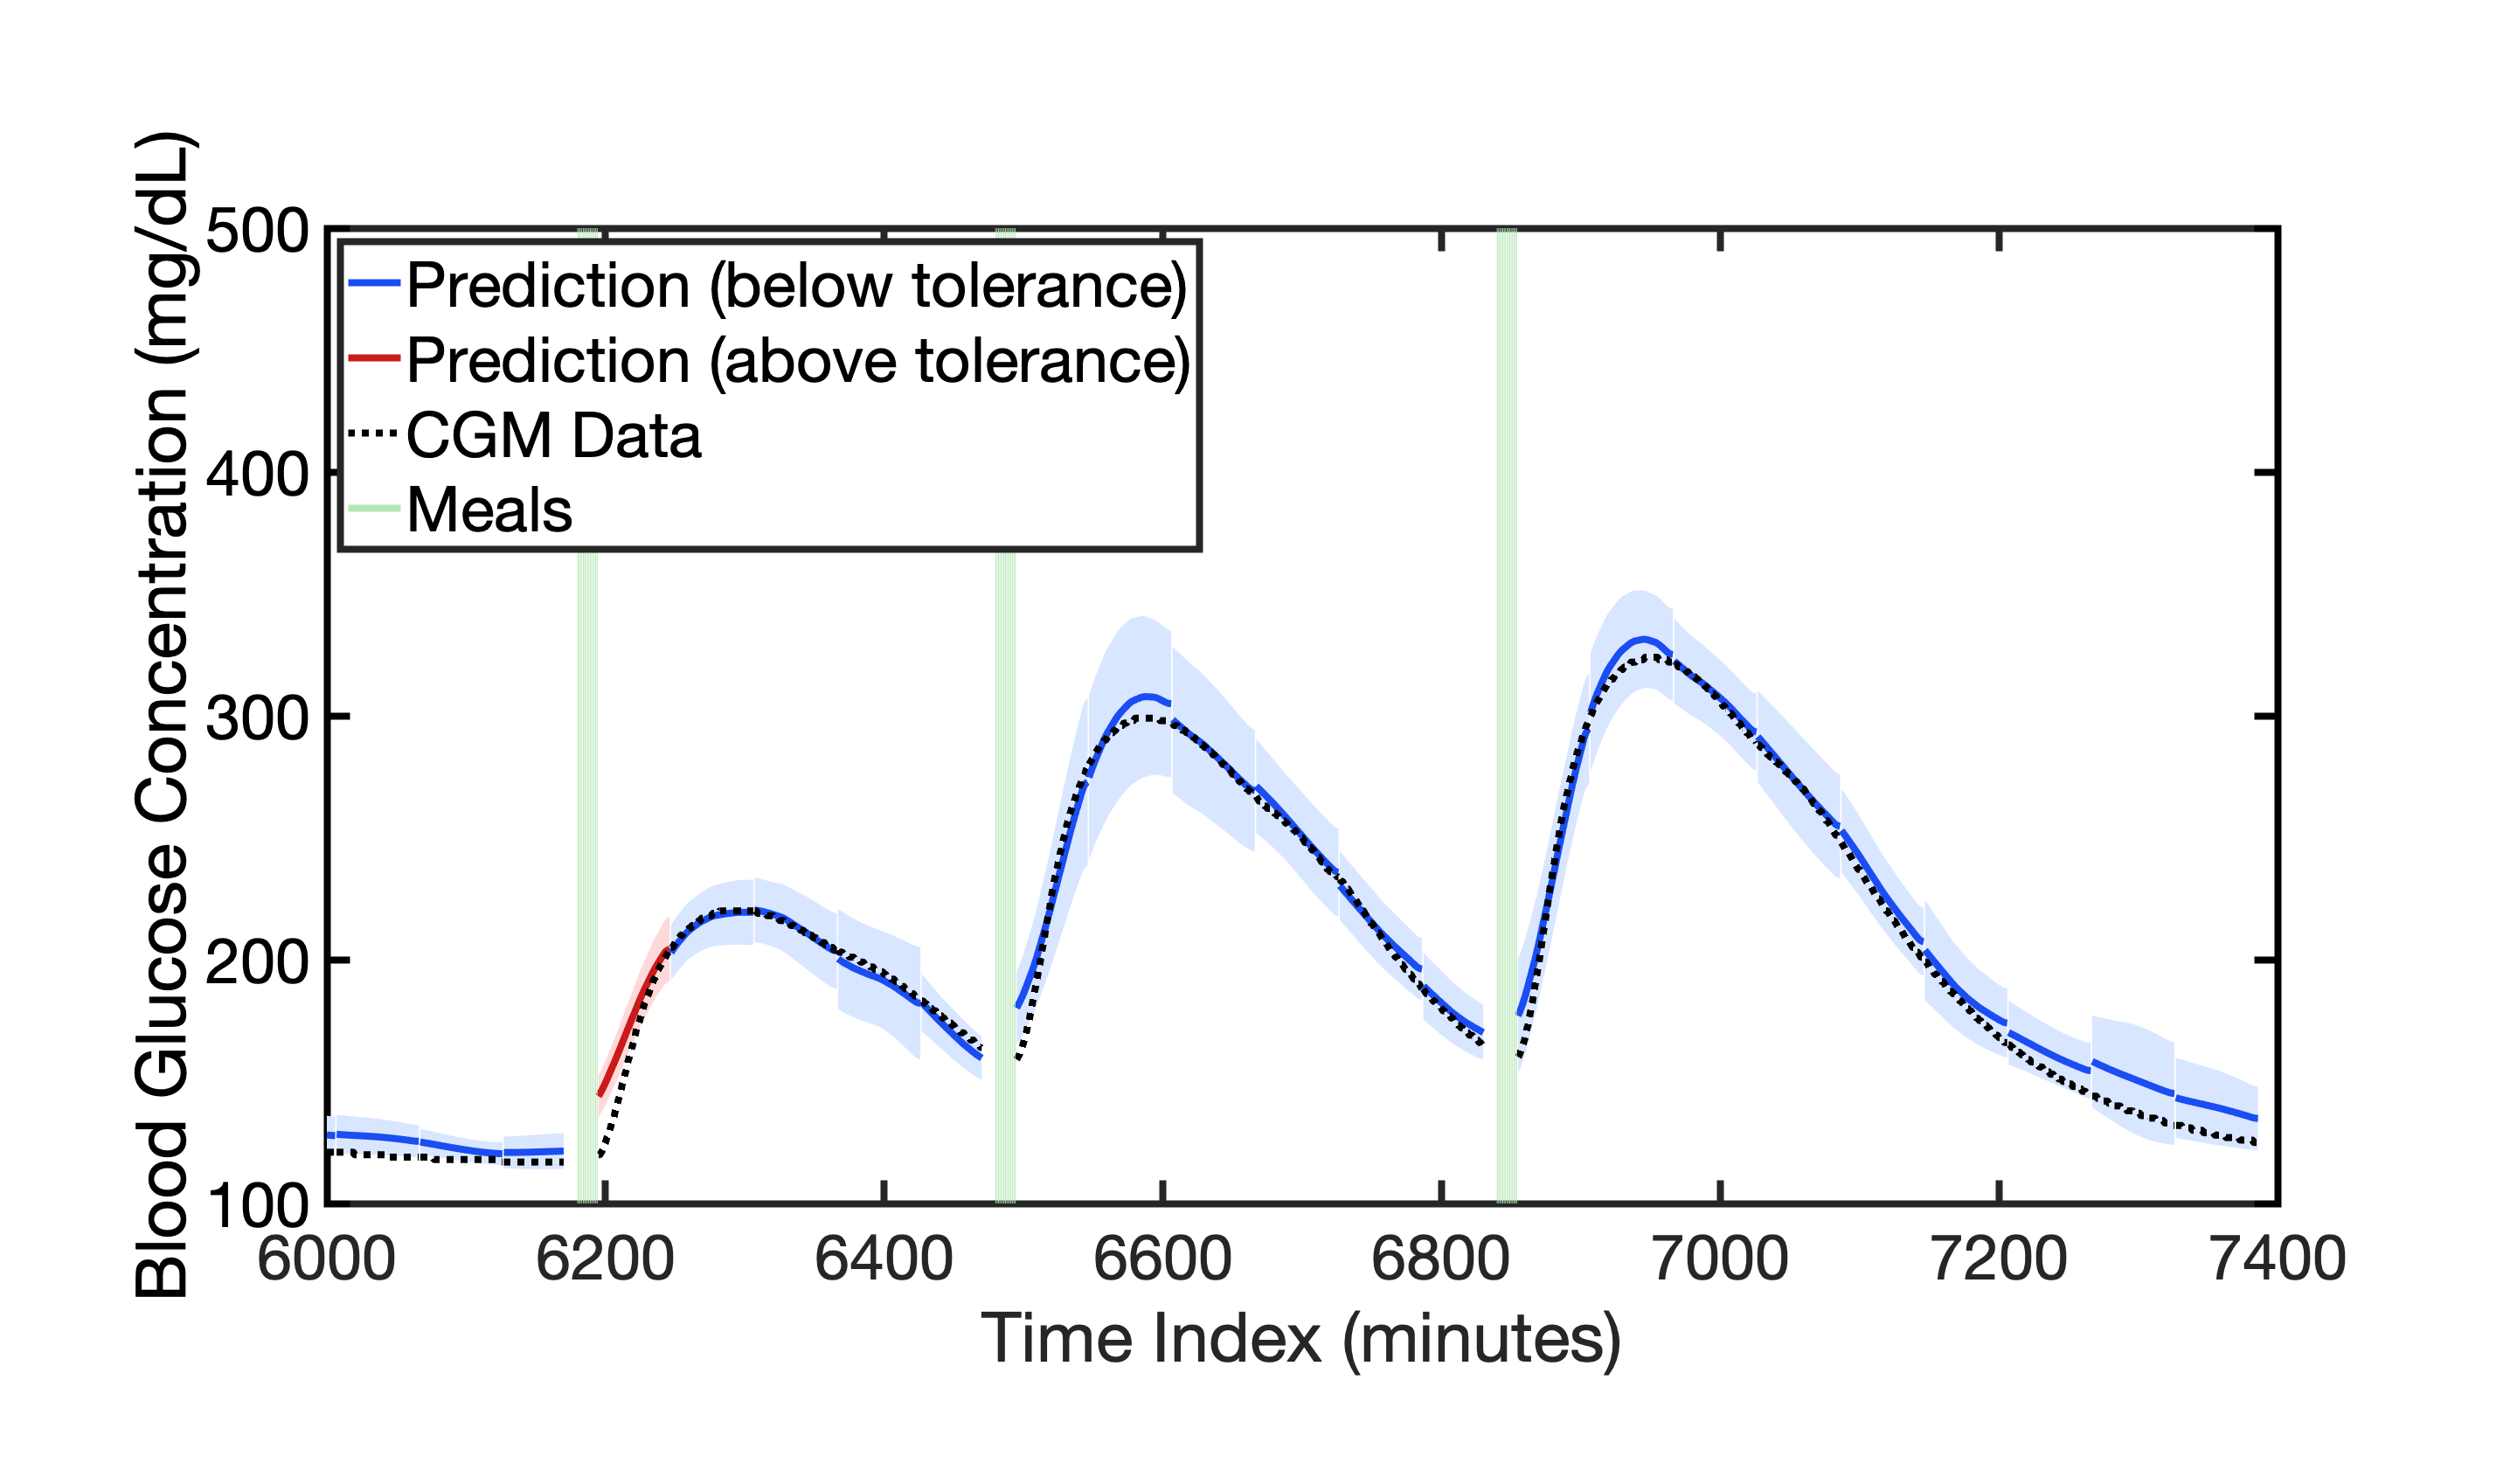
\includegraphics[width=\linewidth]{Figures/Part B/cat2/p6_c2.png}
  \caption*{(a)}
\end{minipage}\hfill
\begin{minipage}[t]{0.48\textwidth}
  \centering
  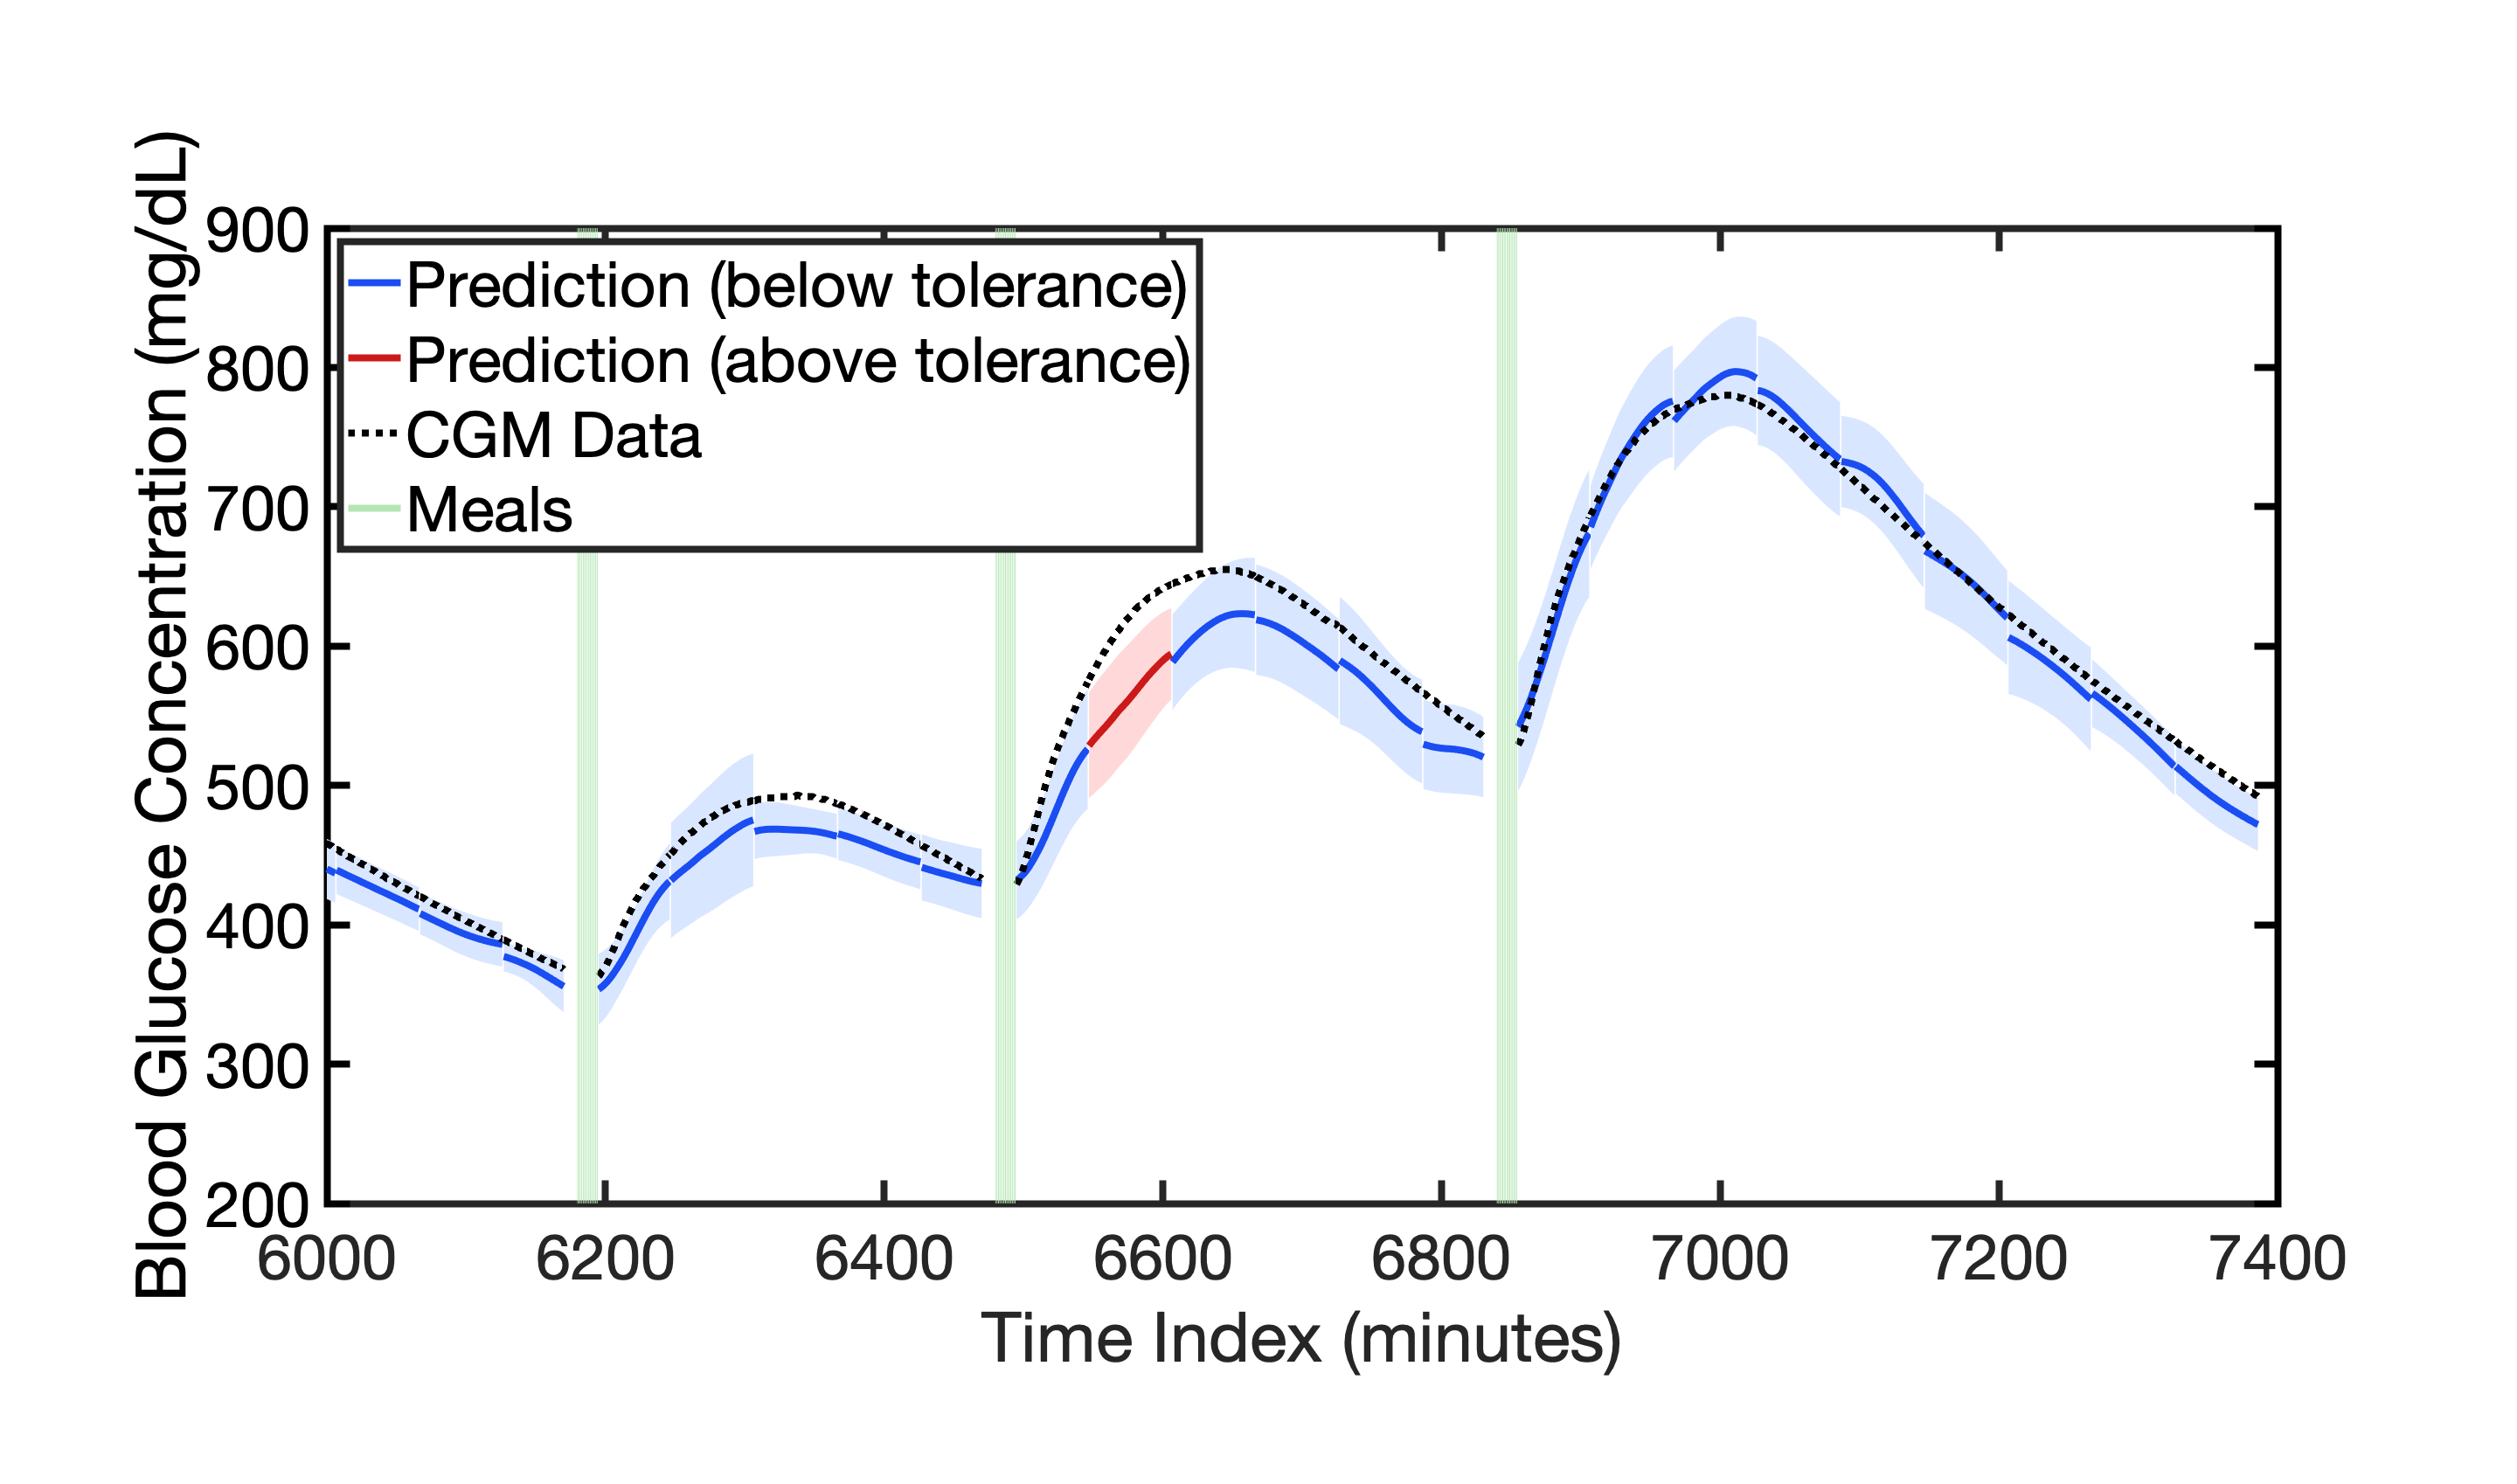
\includegraphics[width=\linewidth]{Figures/Part B/cat2/p7_c2.png}
  \caption*{(b)}
\end{minipage}
%
\begin{minipage}[t]{0.48\textwidth}
  \centering
  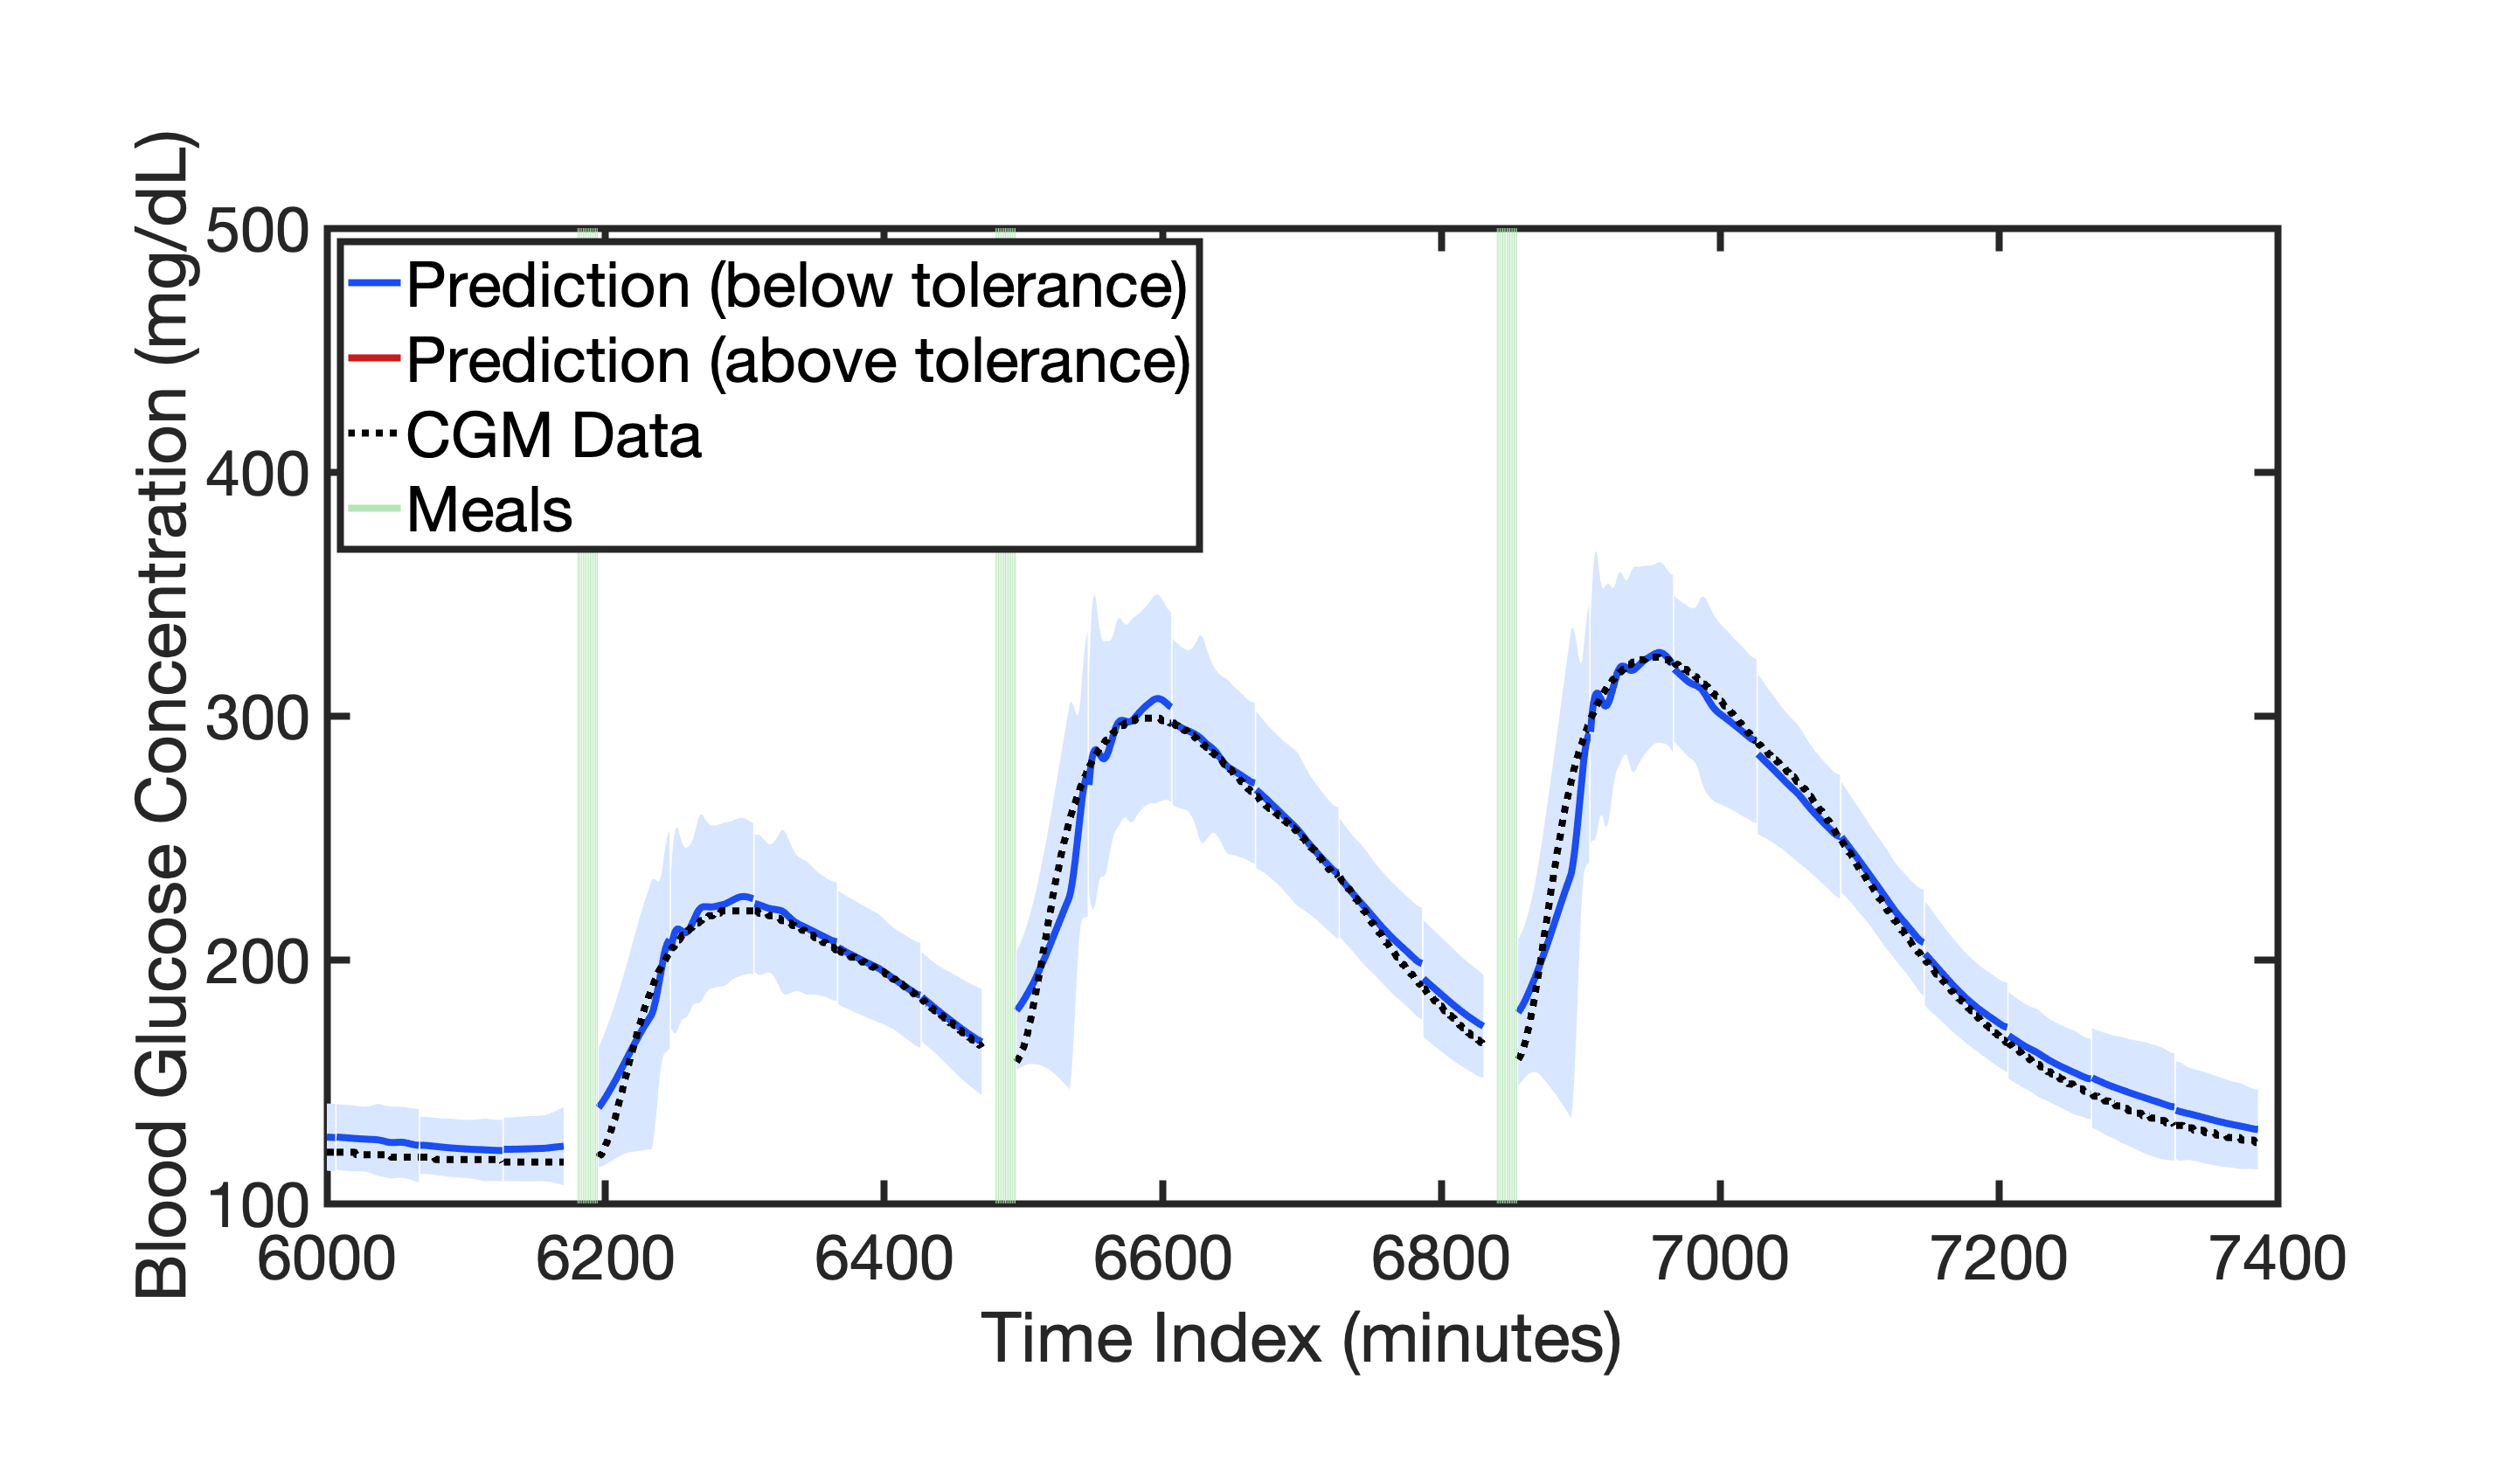
\includegraphics[width=\linewidth]{Figures/Part B/cat2/p6_bma.png}
  \caption*{(c)}
\end{minipage}\hfill
\begin{minipage}[t]{0.48\textwidth}
  \centering
  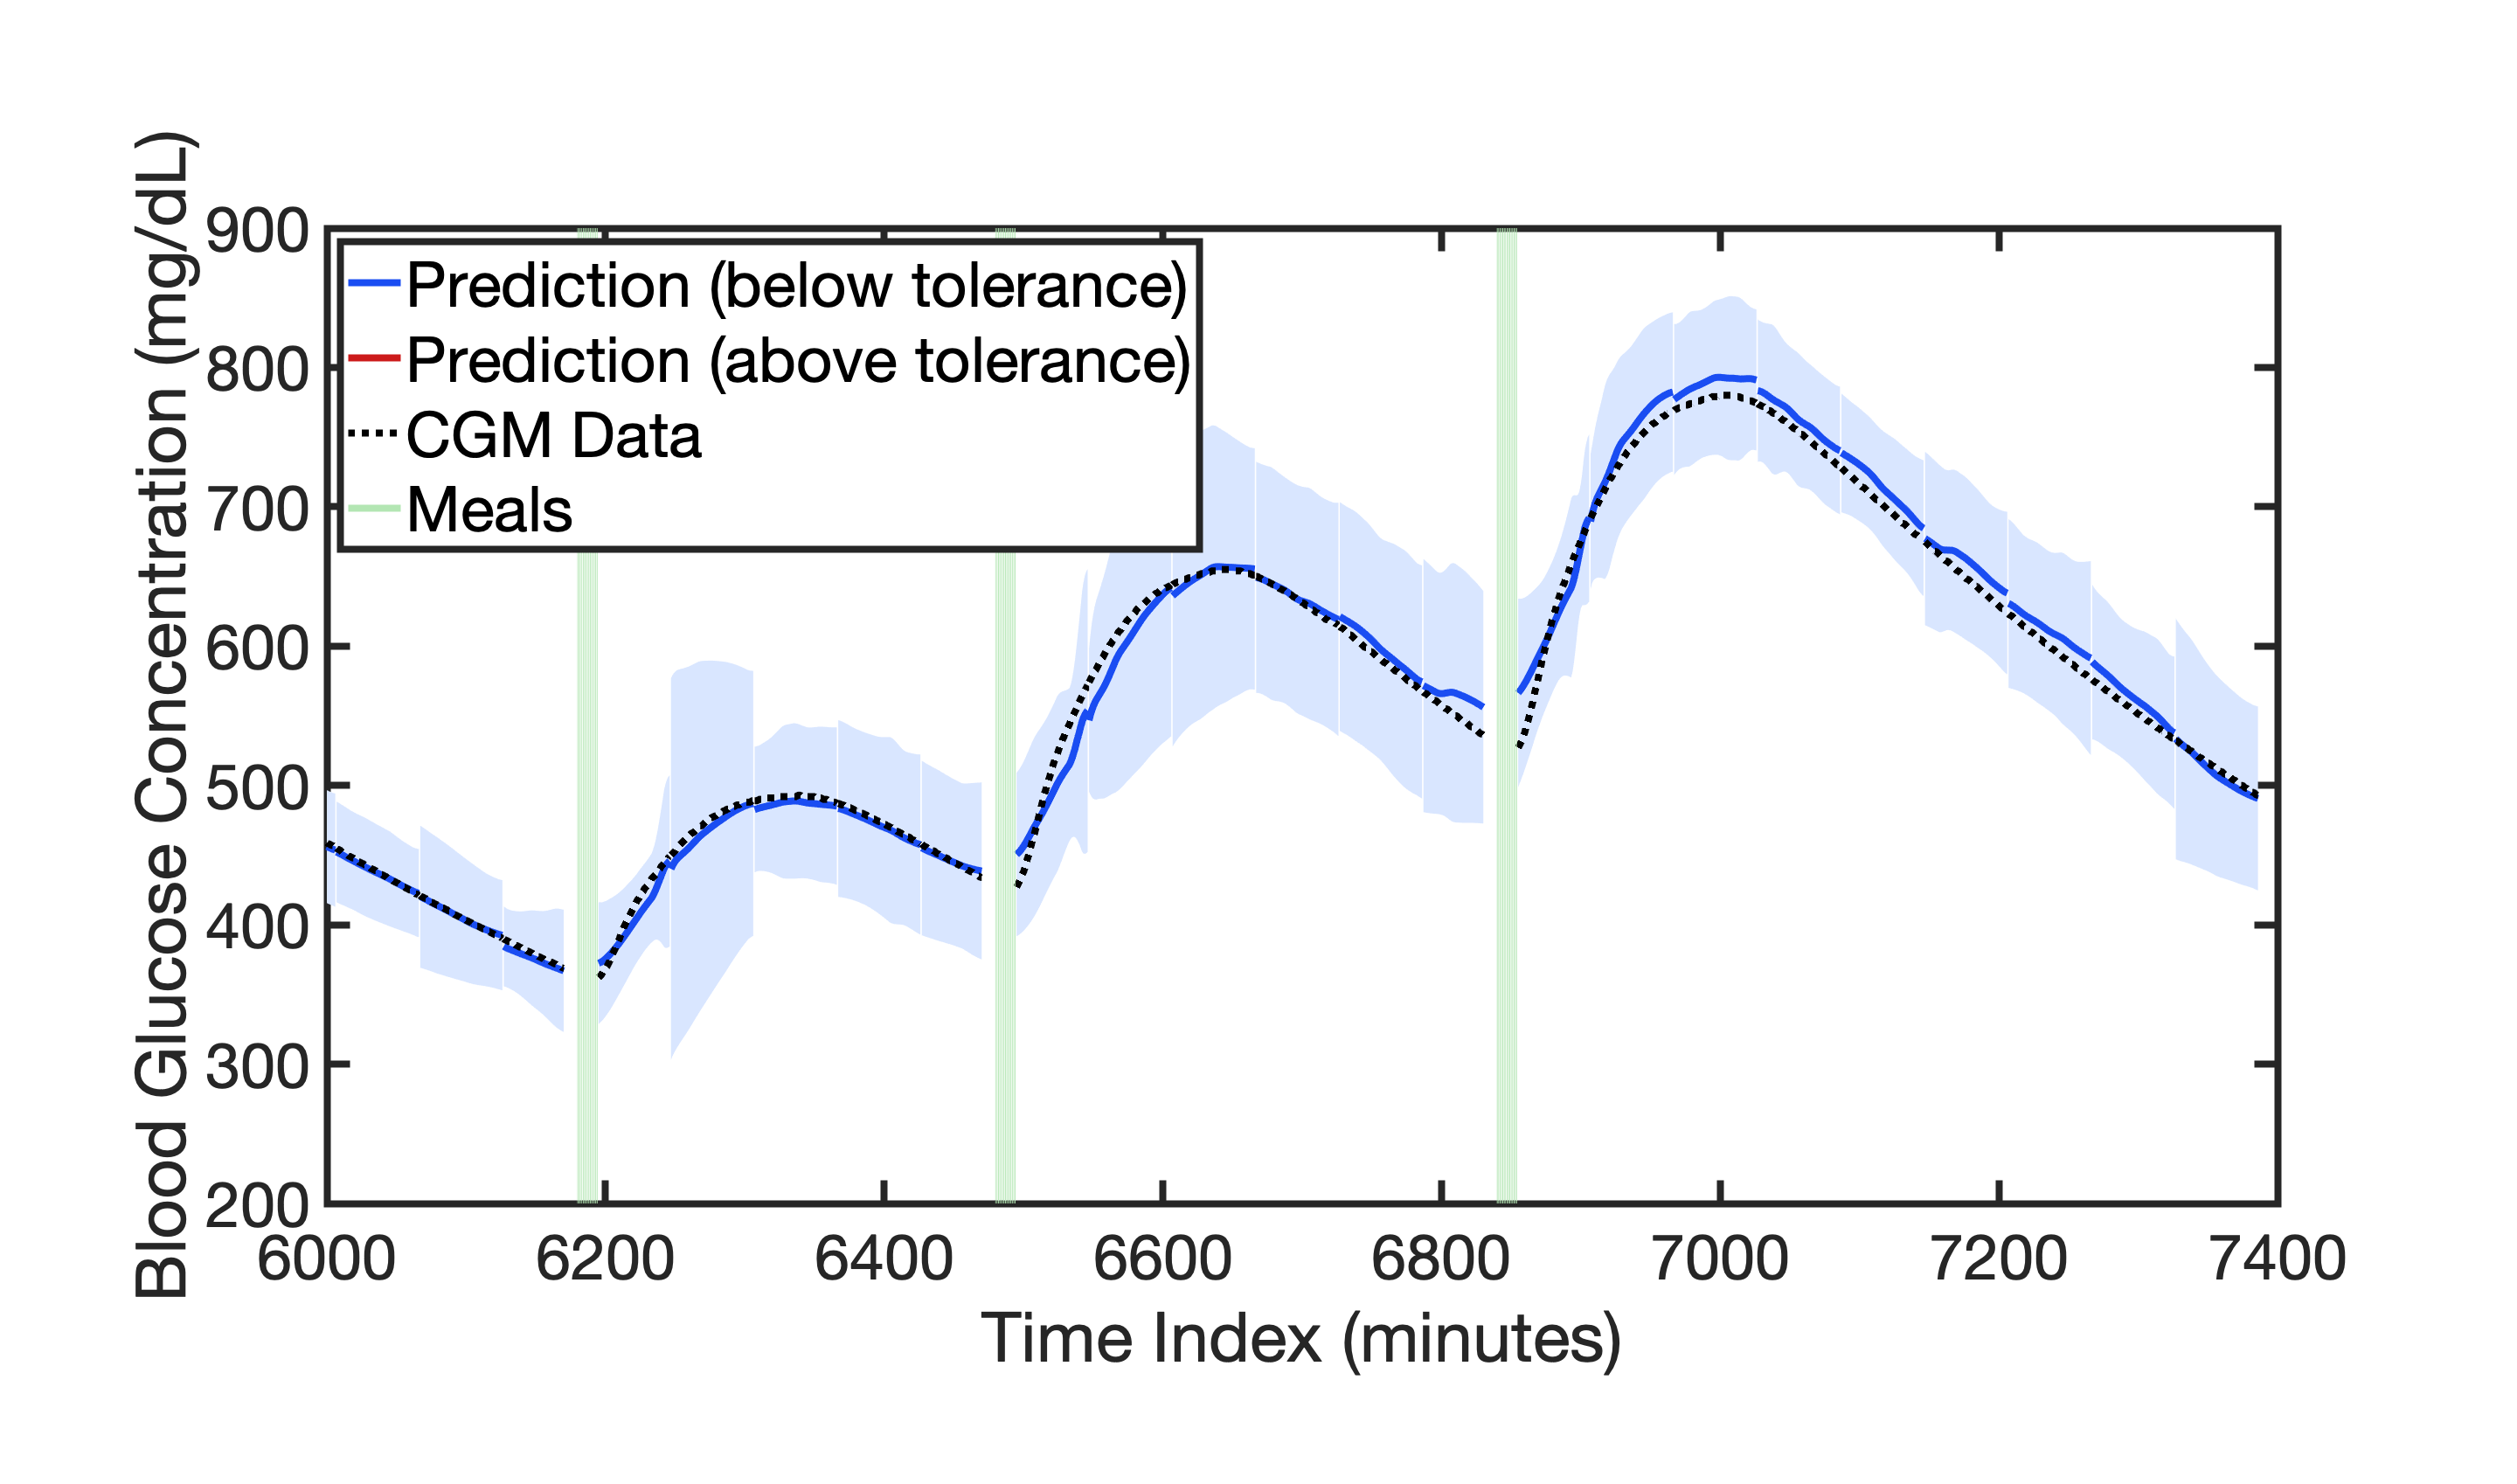
\includegraphics[width=\linewidth]{Figures/Part B/cat2/p7_bma.png}
  \caption*{(d)}
\end{minipage}
\caption{Comparison of single-architecture and plausibility-
weighted ensemble predictions for representative Level~2 candidates in fold~2. 
(a–b) Predictions from a single architecture ($Level_2Arch_7$) for Patients 6–7 in fold~2, and (c–d) corresponding ensemble predictions from all architectures in Level~2.
Red segments indicate one-hour prediction windows that violates the acceptance criterion $NLPD \leq Tol$.}
\label{fig:bma}
\end{figure}





\paragraph{Capacity level 3 ($l=3$)}
Level~3 contains higher-capacity architectures ($10^5$–$4\times10^5$ parameters). Despite their increased representational capacity, these models do not improve validation performance and frequently violate the NLPD criterion across multiple prediction windows (Figure~\ref{fig:pred_cat3}).
The additional parameters at this level are not sufficiently learned by the available data, leading to degraded generalization under inter-patient variability. In contrast to Level~2, where intermediate-capacity architectures satisfy the validation criterion, increasing capacity beyond this regime yields no consistent improvement and introduces  prediction errors.


\begin{figure}[!ht]
\centering
\begin{minipage}[t]{0.48\textwidth}
  \centering
  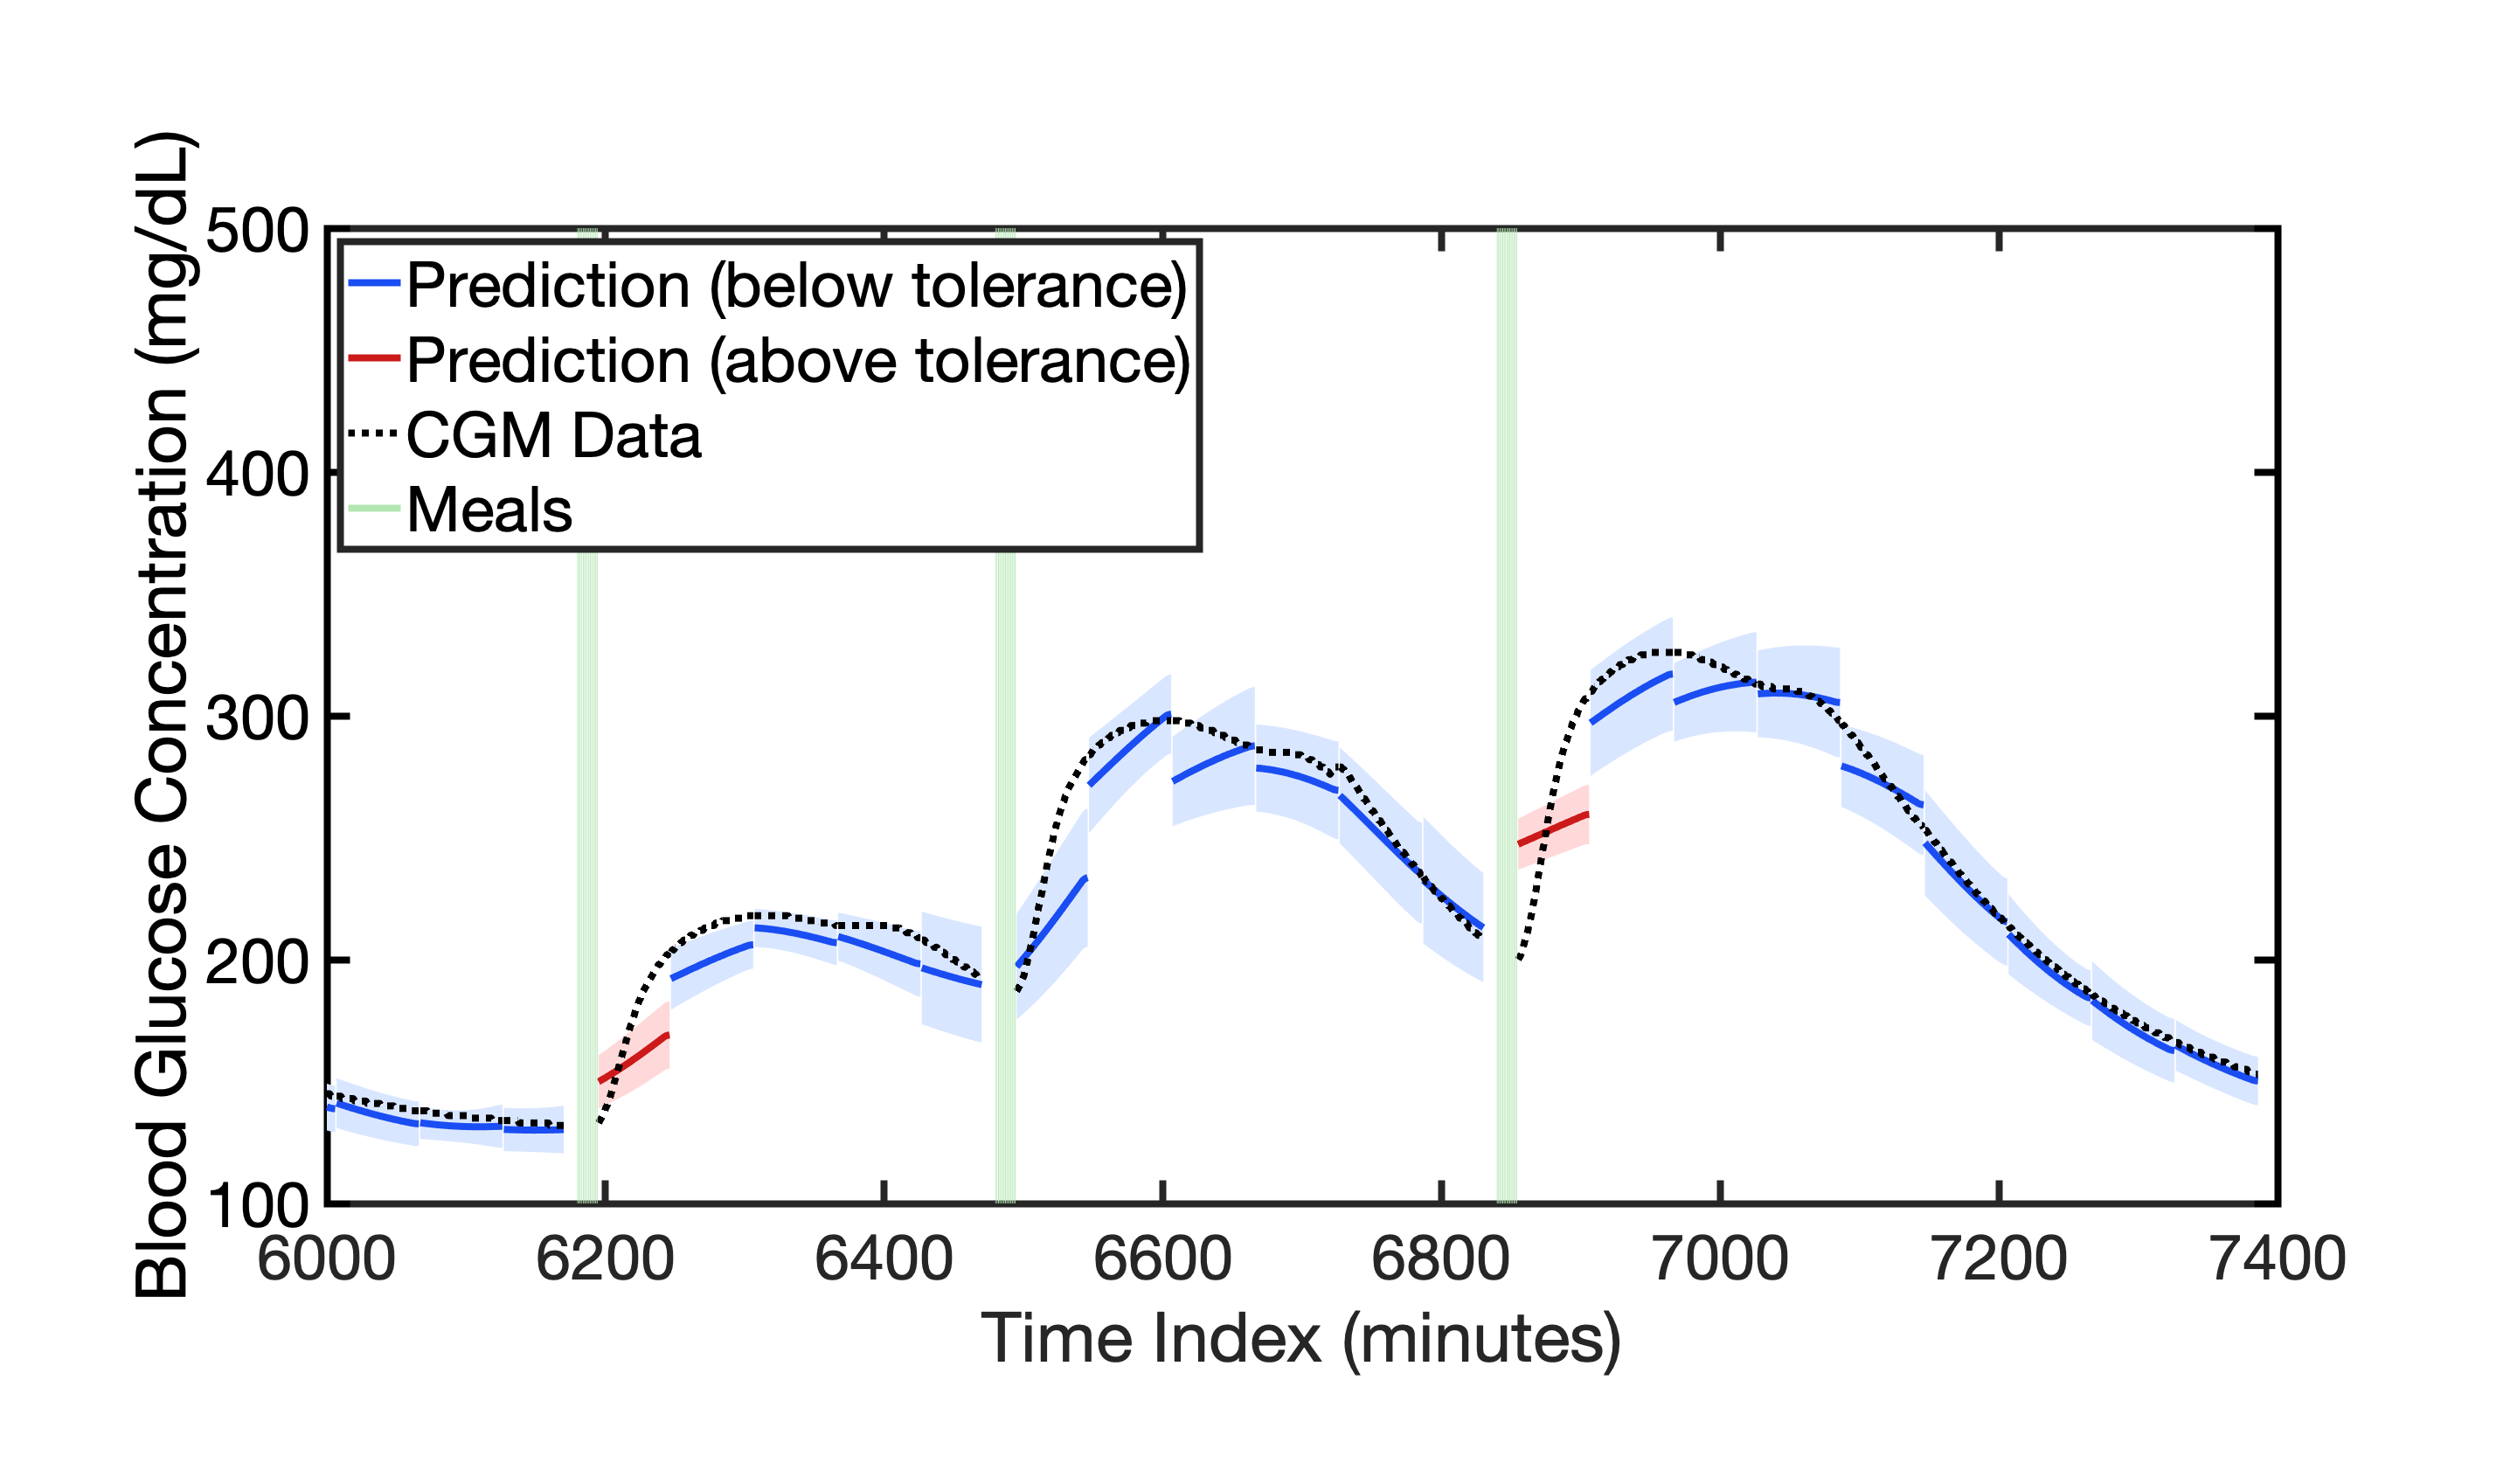
\includegraphics[width=\linewidth]{Figures/Part B/cat3/p1_c3.png}
  \caption*{(a)}
\end{minipage}\hfill
\begin{minipage}[t]{0.48\textwidth}
  \centering
  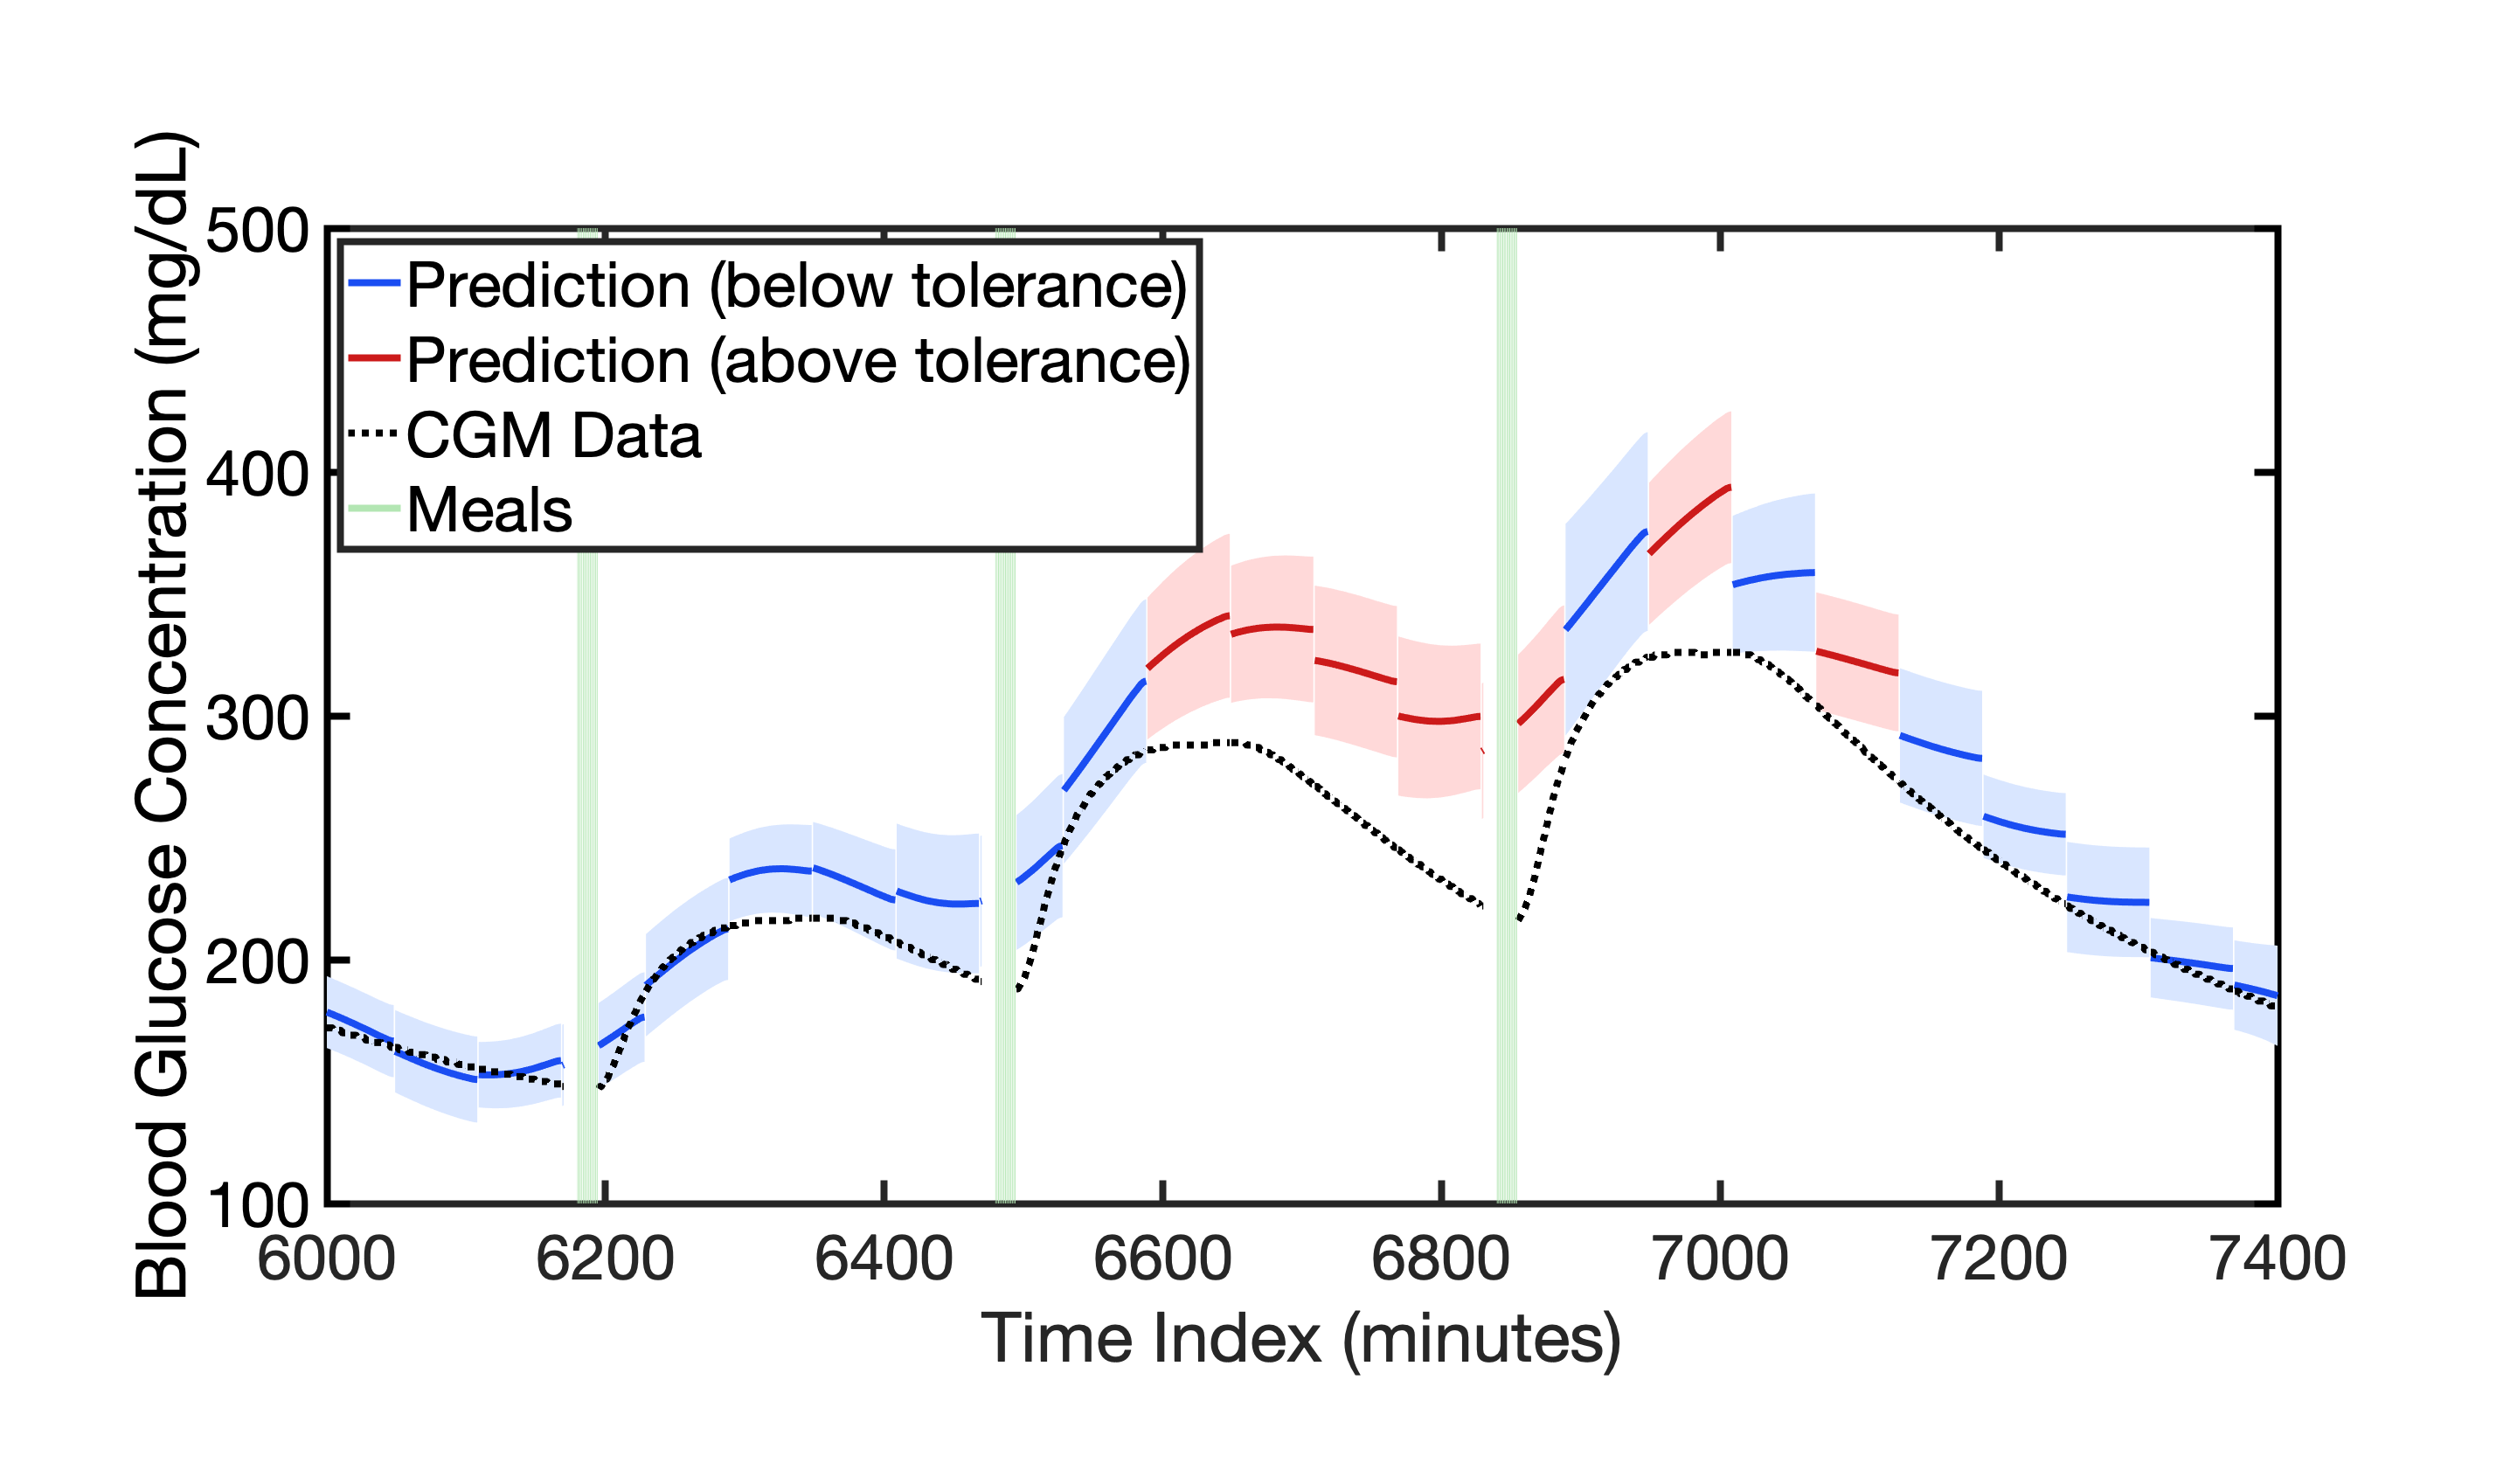
\includegraphics[width=\linewidth]{Figures/Part B/cat3/p4_c3.png}
  \caption*{(b)}
\end{minipage}
\caption{Representative validation failures for Level~3 architectures on held-out patients. (a) Patient 1 from fold~3 using $Level_3Arch_{10}$ and (b) Patient 4 from fold~4 using $Level_3Arch_4$. Red segments indicate one-hour prediction windows that violates the acceptance criterion $NLPD \leq Tol$.}
\label{fig:pred_cat3}
\end{figure}


%----Parks error map
\paragraph{Clinical risk mapping}
To complement NLPD-based validation, we evaluate representative rejected and accepted architectures using the Parkes error grid \cite{parkes2000new, pfutzner2013technical}, a clinically established mapping for assessing the impact of glucose prediction errors on treatment decisions. The grid partitions errors into risk zones including no clinical impact (Zone A). minimal clinical consequence (Zone B), incorrect action affecting
clinical outcome (Zone C), significant medical risk (Zone D), and 
to dangerous treatment decisions (Zone E).
%
Figure~\ref{fig:parkes} compares a rejected Level~1 architecture with the selected Level~2 model. To account for uncertainty, we overlay uncertainty bands from both CGM measurements noise and TCN predictions. While the mean predictions of the Level~1 model appear reasonable, its uncertainty spreads into higher-risk regions (primarily Zone B), indicating potential for clinically suboptimal decisions. In contrast, the selected Level~2 architecture concentrates predictions and associated uncertainty within Zone A, indicating clinically safe behavior. This comparison confirms that EVIDENT’s validation under uncertainty step also aligned with clinically meaningful risk criteria.

\begin{figure}[!ht]
\centering
\begin{minipage}[t]{0.5\textwidth}
  \centering
  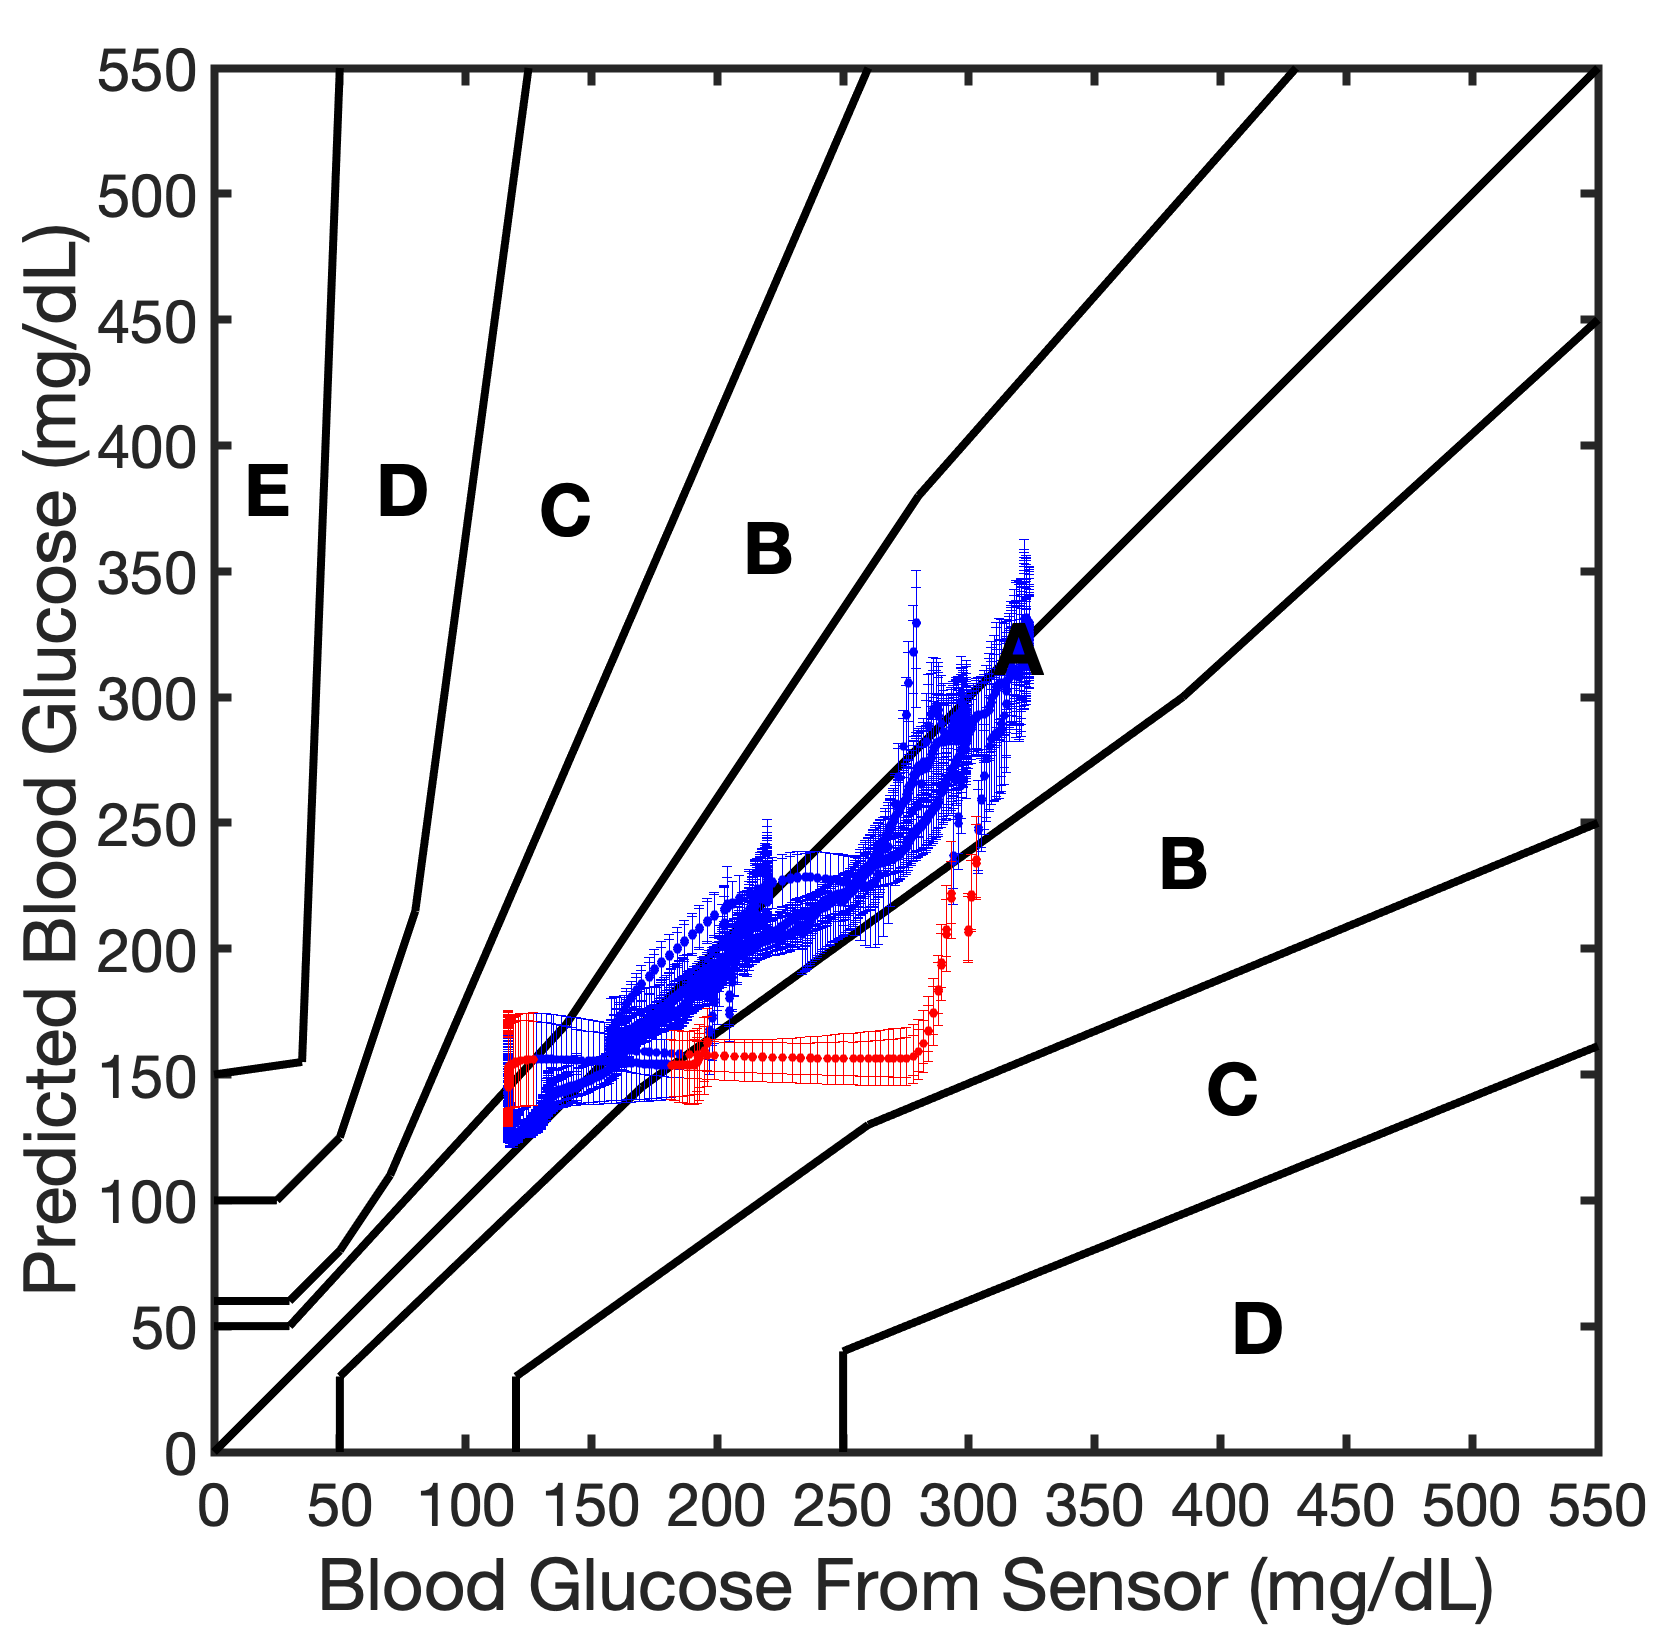
\includegraphics[width=0.8\linewidth]{Figures/results/error_grid_bad.png}
  \caption*{(a)}
\end{minipage}\hfill
\begin{minipage}[t]{0.5\textwidth}
  \centering
 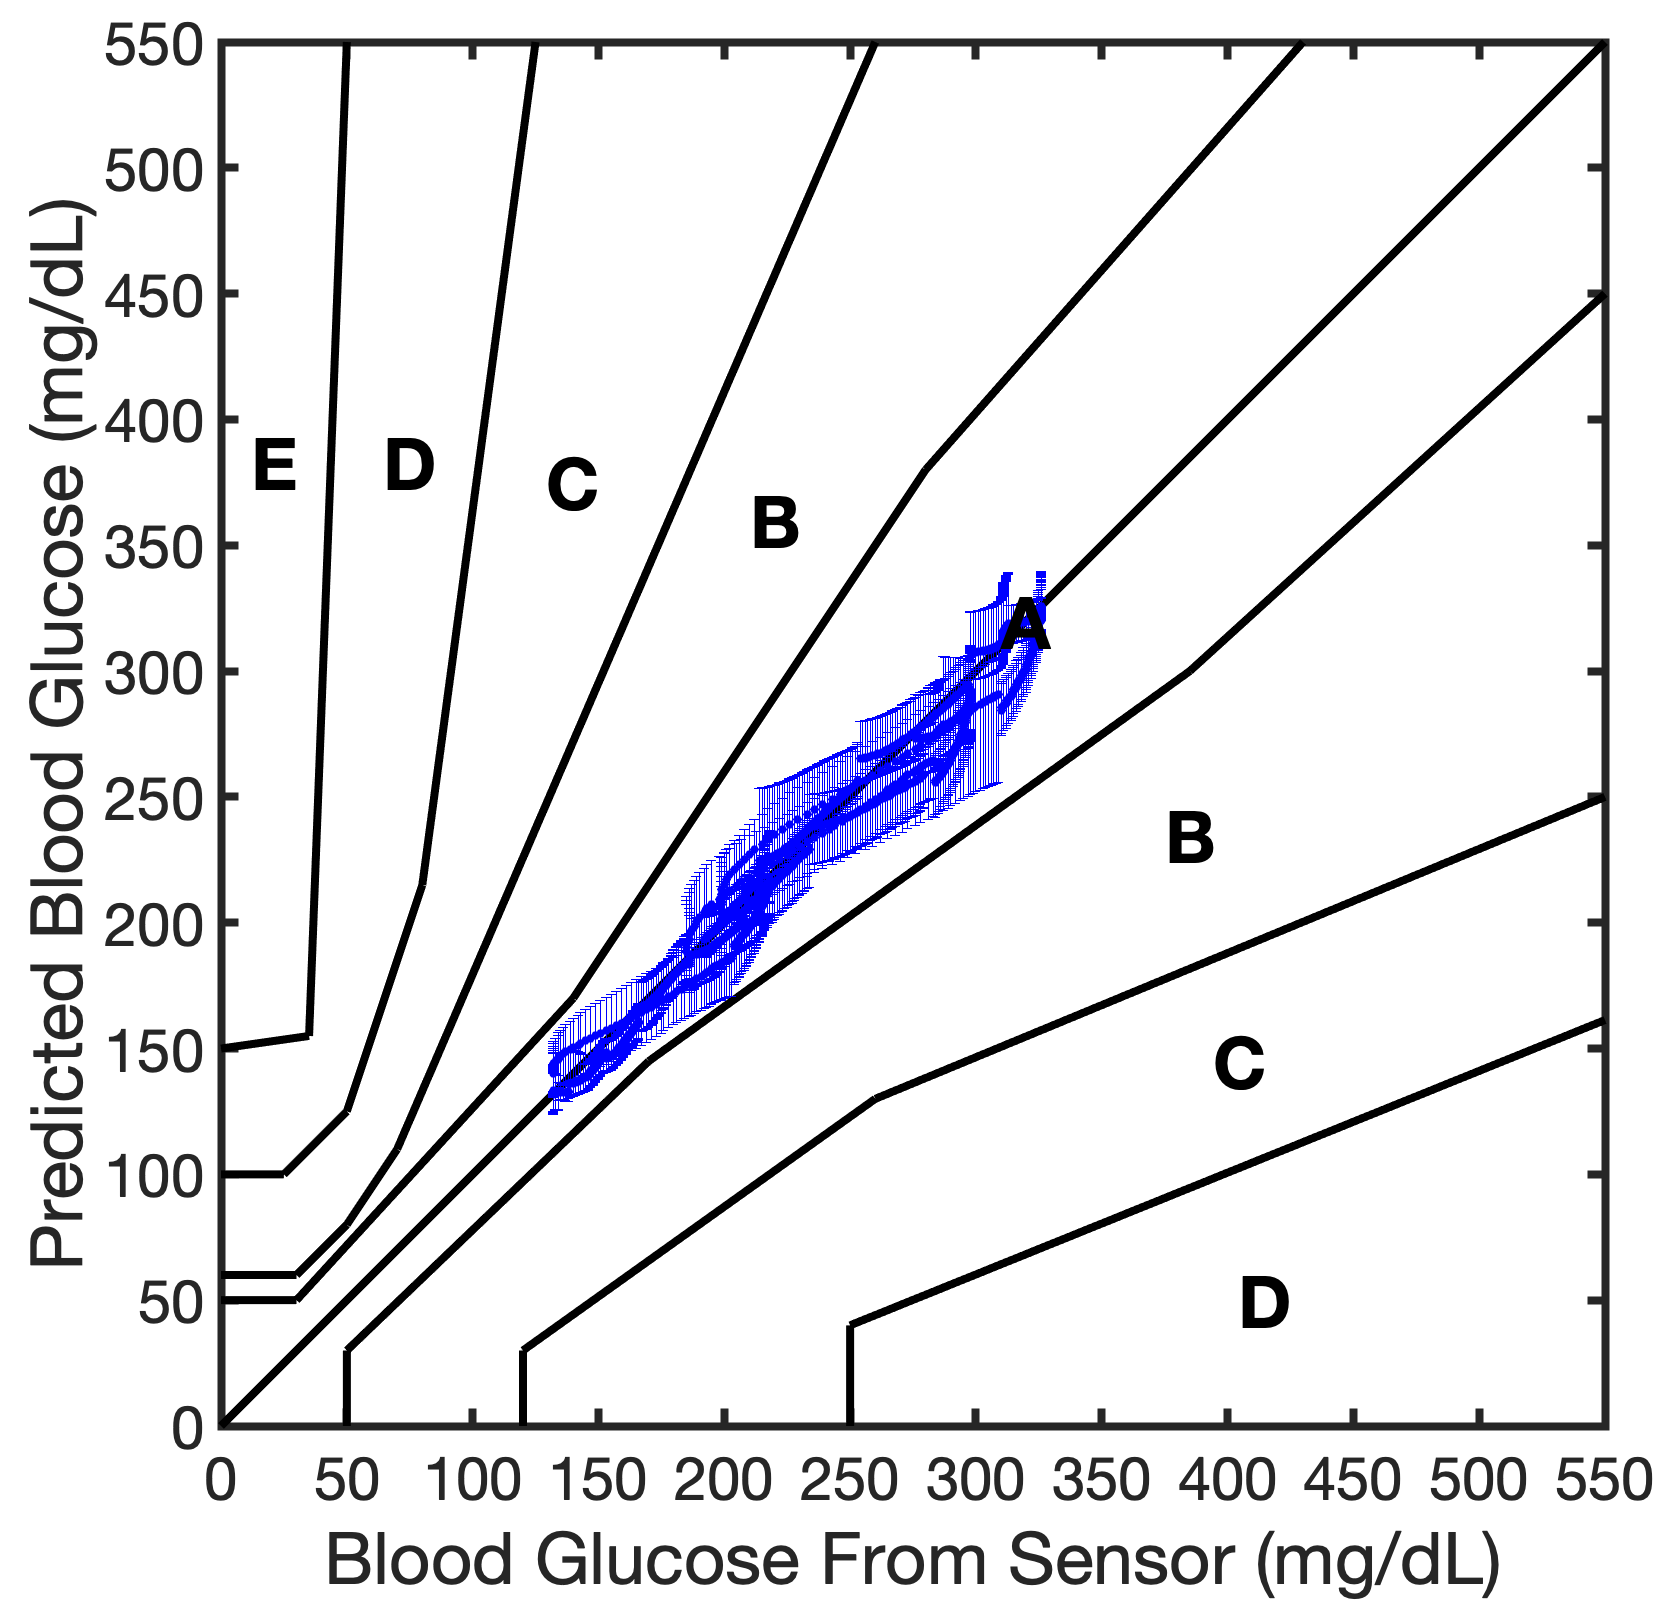
\includegraphics[width=0.8\linewidth]{Figures/results/error_grid_good.png}
  \caption*{(b)}
\end{minipage}
\caption{Clinical risk assessment using the Parkes error grid for representative rejected and accepted architectures by EVIDENT. (a) Rejected Level~1 architecture ($Level\_1Arch\_1$) shows uncertainty extending into higher-risk Zone B. 
(b) Selected Level~2 architecture ($Level\_2Arch\_4$) concentrates predictions within Zone A, corresponding to clinically safe decisions.}
\label{fig:parkes}
\end{figure}




% Discussion
%========================================================
\section{Discussion}\label{sec:discussion}

This study presented an evidence-driven workflow to discover Bayesian TCN (B-TCN) architectures that are credible enough for digital-twin (DT) glucose forecasting, rather than selecting models solely by heuristics such as depth, receptive field, or parameter count. Across the architecture grid, the Bayesian log-evidence (and the derived plausibility ranking) was highly non-uniform, indicating that only a narrow design region achieves a favorable balance between data-fit and complexity. Importantly, the results also show that no single hyperparameter can dominate prediction and high-performing models appear in an intermediate region that is expressive enough to capture meal/insulin dynamics with combination of suitable parameters. 
The present results are based on simulator-generated population data (UVA/Padova adults) and a relatively small patinet set (10 subjects total). The most direct next step is to increase the number of simulated Subjects used for training and validation. As the cohort grows, two improvements are expected: (i) the estimated evidence/plausibility landscape should become more stable (less fold-to-fold fluctuation), and (ii) architectures that currently pass only some folds should be more likely to pass all folds, because training sees a wider range of dynamics and validation becomes less sensitive to idiosyncrasies of two specific patients. In other words, the current fold variability should be viewed primarily as a data-limited effect, not as a fundamental instability of the evidence-based selection principle.


%-------------------------------------------------------
% 1. Summarize the key methods and results (two paragraphs)
%-------------------------------------------------------



%-------------------------------------------------------
% 2. Limitations of the study and possible extensions (one paragraph)
%-------------------------------------------------------


%

%-------------------------------------------------------
% 3. Summarize the main take-home points from the study
%-------------------------------------------------------



%========================================================
% Conclusions
%========================================================
\section{Conclusions}\label{sec:conclusions}

This paper introduced an evidence-driven model discovery workflow for building trustworthy Bayesian TCN surrogate models when only limited initial information is available. Instead of choosing a network by trial-and-error or single metrics (e.g., parameter count or receptive field), we (i) restrict attention to a feasible architecture pool using biological/forecasting constraints (e.g., receptive-field coverage), and then (ii) use Bayesian log-evidence (model plausibility) to rank candidates in a way that naturally balances data-fit and complexity. The selected models are then validated using probabilistic validation (NLPD), so passing models are not only accurate on average but also well-calibrated in uncertainty, which is essential for risk-aware digital-twin use. 

\noindent
Across the population-based T1D study, the results show a clear practical outcome: the most reliable surrogates emerge in an intermediate complexity range. Smaller models tend to underfit glucose excursions, while overly complex models introduce many weakly-informed parameters and generalize less consistently. As the number of training and validation subjects increases, the evidence landscape and validation outcomes are expected to become more stable, and “DT-ready” architectures should be more likely to pass across all folds.



%++++++++++++++++++++++++++++++++++++++++++++++++++++++++++++++++++++++++
\section*{Acknowledgments}
\noindent



%========================================================================
% Appendix
%========================================================================
%% The Appendices part is started with the command \appendix;
%% appendix sections are then done as normal sections
\section{Appendix}\label{sec:appendix}
\begin{footnotesize}
\setlength{\tabcolsep}{6pt}
\begin{longtable}{ccc}
\caption{Different architecture categories}
\label{tab:tcn-arch-paramgrid}\\
\toprule
\textbf{Category} & \textbf{ParamBin} & \textbf{ArchCount} \\
\midrule
\endfirsthead

\toprule
\textbf{ArchName} & \textbf{ParamCount} & \textbf{Layers} & \textbf{Dilation} & \textbf{Filter Size} & \textbf{Encoder Channels} & \textbf{Decoder Channels} \\
\midrule
\endhead

\endfoot

\bottomrule
\endlastfoot
1 & $\le$30k     & 10 \\
2 & 30k--100k    & 9  \\
3 & 100k--400k   & 10 \\
4 & 400k--1M     & 11 \\
5 & 1M--5M       & 11 \\
6 & $\ge$5M      & 10 \\

\end{longtable}
\end{footnotesize}

%========================================================================
% Bibliography
%========================================================================

%% If you have bibdatabase file and want bibtex to generate the
%% bibitems, please use
 \bibliographystyle{elsarticle-num} 
 \bibliography{references}

\end{document}

